% Options for packages loaded elsewhere
% Options for packages loaded elsewhere
\PassOptionsToPackage{unicode}{hyperref}
\PassOptionsToPackage{hyphens}{url}
\PassOptionsToPackage{dvipsnames,svgnames,x11names}{xcolor}
%
\documentclass[
  spanish,
  letterpaper,
]{book}
\usepackage{xcolor}
\usepackage[top=30mm,left=30mm,heightrounded]{geometry}
\usepackage{amsmath,amssymb}
\setcounter{secnumdepth}{5}
\usepackage{iftex}
\ifPDFTeX
  \usepackage[T1]{fontenc}
  \usepackage[utf8]{inputenc}
  \usepackage{textcomp} % provide euro and other symbols
\else % if luatex or xetex
  \usepackage{unicode-math} % this also loads fontspec
  \defaultfontfeatures{Scale=MatchLowercase}
  \defaultfontfeatures[\rmfamily]{Ligatures=TeX,Scale=1}
\fi
\usepackage[]{libertinus}
\ifPDFTeX\else
  % xetex/luatex font selection
\fi
% Use upquote if available, for straight quotes in verbatim environments
\IfFileExists{upquote.sty}{\usepackage{upquote}}{}
\IfFileExists{microtype.sty}{% use microtype if available
  \usepackage[]{microtype}
  \UseMicrotypeSet[protrusion]{basicmath} % disable protrusion for tt fonts
}{}
\makeatletter
\@ifundefined{KOMAClassName}{% if non-KOMA class
  \IfFileExists{parskip.sty}{%
    \usepackage{parskip}
  }{% else
    \setlength{\parindent}{0pt}
    \setlength{\parskip}{6pt plus 2pt minus 1pt}}
}{% if KOMA class
  \KOMAoptions{parskip=half}}
\makeatother
% Make \paragraph and \subparagraph free-standing
\makeatletter
\ifx\paragraph\undefined\else
  \let\oldparagraph\paragraph
  \renewcommand{\paragraph}{
    \@ifstar
      \xxxParagraphStar
      \xxxParagraphNoStar
  }
  \newcommand{\xxxParagraphStar}[1]{\oldparagraph*{#1}\mbox{}}
  \newcommand{\xxxParagraphNoStar}[1]{\oldparagraph{#1}\mbox{}}
\fi
\ifx\subparagraph\undefined\else
  \let\oldsubparagraph\subparagraph
  \renewcommand{\subparagraph}{
    \@ifstar
      \xxxSubParagraphStar
      \xxxSubParagraphNoStar
  }
  \newcommand{\xxxSubParagraphStar}[1]{\oldsubparagraph*{#1}\mbox{}}
  \newcommand{\xxxSubParagraphNoStar}[1]{\oldsubparagraph{#1}\mbox{}}
\fi
\makeatother

\usepackage{color}
\usepackage{fancyvrb}
\newcommand{\VerbBar}{|}
\newcommand{\VERB}{\Verb[commandchars=\\\{\}]}
\DefineVerbatimEnvironment{Highlighting}{Verbatim}{commandchars=\\\{\}}
% Add ',fontsize=\small' for more characters per line
\usepackage{framed}
\definecolor{shadecolor}{RGB}{241,243,245}
\newenvironment{Shaded}{\begin{snugshade}}{\end{snugshade}}
\newcommand{\AlertTok}[1]{\textcolor[rgb]{0.68,0.00,0.00}{#1}}
\newcommand{\AnnotationTok}[1]{\textcolor[rgb]{0.37,0.37,0.37}{#1}}
\newcommand{\AttributeTok}[1]{\textcolor[rgb]{0.40,0.45,0.13}{#1}}
\newcommand{\BaseNTok}[1]{\textcolor[rgb]{0.68,0.00,0.00}{#1}}
\newcommand{\BuiltInTok}[1]{\textcolor[rgb]{0.00,0.23,0.31}{#1}}
\newcommand{\CharTok}[1]{\textcolor[rgb]{0.13,0.47,0.30}{#1}}
\newcommand{\CommentTok}[1]{\textcolor[rgb]{0.37,0.37,0.37}{#1}}
\newcommand{\CommentVarTok}[1]{\textcolor[rgb]{0.37,0.37,0.37}{\textit{#1}}}
\newcommand{\ConstantTok}[1]{\textcolor[rgb]{0.56,0.35,0.01}{#1}}
\newcommand{\ControlFlowTok}[1]{\textcolor[rgb]{0.00,0.23,0.31}{\textbf{#1}}}
\newcommand{\DataTypeTok}[1]{\textcolor[rgb]{0.68,0.00,0.00}{#1}}
\newcommand{\DecValTok}[1]{\textcolor[rgb]{0.68,0.00,0.00}{#1}}
\newcommand{\DocumentationTok}[1]{\textcolor[rgb]{0.37,0.37,0.37}{\textit{#1}}}
\newcommand{\ErrorTok}[1]{\textcolor[rgb]{0.68,0.00,0.00}{#1}}
\newcommand{\ExtensionTok}[1]{\textcolor[rgb]{0.00,0.23,0.31}{#1}}
\newcommand{\FloatTok}[1]{\textcolor[rgb]{0.68,0.00,0.00}{#1}}
\newcommand{\FunctionTok}[1]{\textcolor[rgb]{0.28,0.35,0.67}{#1}}
\newcommand{\ImportTok}[1]{\textcolor[rgb]{0.00,0.46,0.62}{#1}}
\newcommand{\InformationTok}[1]{\textcolor[rgb]{0.37,0.37,0.37}{#1}}
\newcommand{\KeywordTok}[1]{\textcolor[rgb]{0.00,0.23,0.31}{\textbf{#1}}}
\newcommand{\NormalTok}[1]{\textcolor[rgb]{0.00,0.23,0.31}{#1}}
\newcommand{\OperatorTok}[1]{\textcolor[rgb]{0.37,0.37,0.37}{#1}}
\newcommand{\OtherTok}[1]{\textcolor[rgb]{0.00,0.23,0.31}{#1}}
\newcommand{\PreprocessorTok}[1]{\textcolor[rgb]{0.68,0.00,0.00}{#1}}
\newcommand{\RegionMarkerTok}[1]{\textcolor[rgb]{0.00,0.23,0.31}{#1}}
\newcommand{\SpecialCharTok}[1]{\textcolor[rgb]{0.37,0.37,0.37}{#1}}
\newcommand{\SpecialStringTok}[1]{\textcolor[rgb]{0.13,0.47,0.30}{#1}}
\newcommand{\StringTok}[1]{\textcolor[rgb]{0.13,0.47,0.30}{#1}}
\newcommand{\VariableTok}[1]{\textcolor[rgb]{0.07,0.07,0.07}{#1}}
\newcommand{\VerbatimStringTok}[1]{\textcolor[rgb]{0.13,0.47,0.30}{#1}}
\newcommand{\WarningTok}[1]{\textcolor[rgb]{0.37,0.37,0.37}{\textit{#1}}}

\usepackage{longtable,booktabs,array}
\usepackage{calc} % for calculating minipage widths
% Correct order of tables after \paragraph or \subparagraph
\usepackage{etoolbox}
\makeatletter
\patchcmd\longtable{\par}{\if@noskipsec\mbox{}\fi\par}{}{}
\makeatother
% Allow footnotes in longtable head/foot
\IfFileExists{footnotehyper.sty}{\usepackage{footnotehyper}}{\usepackage{footnote}}
\makesavenoteenv{longtable}
\usepackage{graphicx}
\makeatletter
\newsavebox\pandoc@box
\newcommand*\pandocbounded[1]{% scales image to fit in text height/width
  \sbox\pandoc@box{#1}%
  \Gscale@div\@tempa{\textheight}{\dimexpr\ht\pandoc@box+\dp\pandoc@box\relax}%
  \Gscale@div\@tempb{\linewidth}{\wd\pandoc@box}%
  \ifdim\@tempb\p@<\@tempa\p@\let\@tempa\@tempb\fi% select the smaller of both
  \ifdim\@tempa\p@<\p@\scalebox{\@tempa}{\usebox\pandoc@box}%
  \else\usebox{\pandoc@box}%
  \fi%
}
% Set default figure placement to htbp
\def\fps@figure{htbp}
\makeatother



\ifLuaTeX
\usepackage[bidi=basic]{babel}
\else
\usepackage[bidi=default]{babel}
\fi
% get rid of language-specific shorthands (see #6817):
\let\LanguageShortHands\languageshorthands
\def\languageshorthands#1{}


\setlength{\emergencystretch}{3em} % prevent overfull lines

\providecommand{\tightlist}{%
  \setlength{\itemsep}{0pt}\setlength{\parskip}{0pt}}



 
\usepackage[]{biblatex}
\addbibresource{references.bib}


\makeatletter
\@ifpackageloaded{bookmark}{}{\usepackage{bookmark}}
\makeatother
\makeatletter
\@ifpackageloaded{caption}{}{\usepackage{caption}}
\AtBeginDocument{%
\ifdefined\contentsname
  \renewcommand*\contentsname{Tabla de contenidos}
\else
  \newcommand\contentsname{Tabla de contenidos}
\fi
\ifdefined\listfigurename
  \renewcommand*\listfigurename{Listado de Figuras}
\else
  \newcommand\listfigurename{Listado de Figuras}
\fi
\ifdefined\listtablename
  \renewcommand*\listtablename{Listado de Tablas}
\else
  \newcommand\listtablename{Listado de Tablas}
\fi
\ifdefined\figurename
  \renewcommand*\figurename{Figura}
\else
  \newcommand\figurename{Figura}
\fi
\ifdefined\tablename
  \renewcommand*\tablename{Tabla}
\else
  \newcommand\tablename{Tabla}
\fi
}
\@ifpackageloaded{float}{}{\usepackage{float}}
\floatstyle{ruled}
\@ifundefined{c@chapter}{\newfloat{codelisting}{h}{lop}}{\newfloat{codelisting}{h}{lop}[chapter]}
\floatname{codelisting}{Listado}
\newcommand*\listoflistings{\listof{codelisting}{Listado de Listados}}
\makeatother
\makeatletter
\makeatother
\makeatletter
\@ifpackageloaded{caption}{}{\usepackage{caption}}
\@ifpackageloaded{subcaption}{}{\usepackage{subcaption}}
\makeatother
\usepackage{bookmark}
\IfFileExists{xurl.sty}{\usepackage{xurl}}{} % add URL line breaks if available
\urlstyle{same}
\hypersetup{
  pdftitle={R para el Análisis Estadístico de Datos Agrícolas},
  pdfauthor={P. Agr. Ludwing Isaí Marroquín Jiménez},
  pdflang={es},
  colorlinks=true,
  linkcolor={Maroon},
  filecolor={Maroon},
  citecolor={Blue},
  urlcolor={Blue},
  pdfcreator={LaTeX via pandoc}}


\title{R para el Análisis Estadístico de Datos Agrícolas}
\author{P. Agr. Ludwing Isaí Marroquín Jiménez}
\date{27 jun 2025}
\begin{document}
\frontmatter
\maketitle

\renewcommand*\contentsname{Tabla de contenidos}
{
\hypersetup{linkcolor=}
\setcounter{tocdepth}{2}
\tableofcontents
}
\listoffigures
\listoftables

\mainmatter
\bookmarksetup{startatroot}

\chapter*{Introducción}\label{introducciuxf3n}
\addcontentsline{toc}{chapter}{Introducción}

\markboth{Introducción}{Introducción}

En el ámbito de la investigación agronómica, la estadística se presenta
como una herramienta esencial para la transformación de datos en
conocimiento aplicable. Este manual, titulado `R para el Análisis
Estadístico de Datos Agrícolas', ha sido concebido como una introducción
accesible y práctica al análisis estadístico moderno, con un enfoque
particular en el lenguaje R.

Tradicionalmente, la estadística ha proporcionado los cimientos para la
toma de decisiones informadas en la agricultura. Sin embargo, la
creciente disponibilidad de datos y la necesidad de análisis más
sofisticados exigen un enfoque actualizado y eficiente. R, un lenguaje
de programación y entorno de software ampliamente adoptado en la ciencia
de datos y la estadística aplicada, ofrece la flexibilidad y el poder
necesarios para abordar estos desafíos (Ihaka \& Gentleman, 1996; R Core
Team, 2023).

Este manual está diseñado para guiar al lector a través de un proceso
gradual y comprensible, desde los conceptos estadísticos fundamentales
hasta las técnicas esenciales para el análisis estadístico de datos
agrícolas. Se abordan temas clave como aspectos introductorios,
clasificación de variables, notación sumatoria, medidas de tendencia
central y dispersión (tanto para datos agrupados como no agrupados),
introducción a probabilidades, distribuciones de probabilidad discretas,
la distribución normal, intervalos de confianza, pruebas de hipótesis, y
regresión lineal y correlación.

Cada capítulo combina la teoría con ejemplos prácticos y estudios de
caso relevantes, facilitando la comprensión y la aplicación de los
métodos en situaciones reales. El propósito central es proporcionar una
base sólida que permita a los profesionales y estudiantes de agronomía
utilizar R de manera efectiva en su trabajo diario. No se requiere
experiencia previa en programación o estadística; el manual está
estructurado para ser accesible a todos, independientemente de su nivel
de conocimientos iniciales.

\section*{Organización del manual}\label{organizaciuxf3n-del-manual}
\addcontentsline{toc}{section}{Organización del manual}

\markright{Organización del manual}

El presente manual se estructura de manera progresiva, comenzando con
los fundamentos esenciales y avanzando hacia técnicas estadísticas
aplicadas, con el objetivo de facilitar una comprensión integral del
análisis estadístico de datos agrícolas utilizando R. Cada capítulo
incluye explicaciones detalladas, ejemplos prácticos y código R
reproducible, diseñados para consolidar el aprendizaje y fomentar la
aplicación efectiva de los conceptos.

A continuación, se presenta una tabla que resume la organización del
manual, detallando los temas cubiertos en cada capítulo:

\begin{longtable}[]{@{}
  >{\raggedright\arraybackslash}p{(\linewidth - 4\tabcolsep) * \real{0.3333}}
  >{\raggedright\arraybackslash}p{(\linewidth - 4\tabcolsep) * \real{0.3333}}
  >{\raggedright\arraybackslash}p{(\linewidth - 4\tabcolsep) * \real{0.3333}}@{}}
\toprule\noalign{}
\begin{minipage}[b]{\linewidth}\raggedright
Capítulo
\end{minipage} & \begin{minipage}[b]{\linewidth}\raggedright
Título
\end{minipage} & \begin{minipage}[b]{\linewidth}\raggedright
Descripción
\end{minipage} \\
\midrule\noalign{}
\endhead
\bottomrule\noalign{}
\endlastfoot
1 & Aspectos introductorios & Introducción a la estadística, su
importancia en agronomía y primeros pasos en R y RStudio. \\
2 & Clasificación de variables & Tipos de variables, escalas de medición
y ejemplos aplicados al ámbito agrícola. \\
3 & Notación sumatoria & Fundamentos y aplicaciones de la notación
sumatoria en el cálculo de estadísticos descriptivos. \\
4 & Medidas de tendencia central y dispersión (datos no agrupados) &
Cálculo e interpretación de media, mediana, moda, rango, varianza y
desviación estándar para datos no agrupados. \\
5 & Medidas de tendencia central y dispersión (datos agrupados) &
Aplicación de medidas de tendencia central y dispersión en tablas de
frecuencia utilizando R. \\
6 & Introducción a probabilidades & Conceptos básicos de probabilidad,
espacio muestral, eventos y reglas de probabilidad. \\
7 & Distribuciones de probabilidad discretas & Estudio de las
distribuciones binomial y Poisson, cálculo de probabilidades y
representación gráfica en R. \\
8 & Distribución normal & Propiedades y aplicaciones de la distribución
normal, cálculo de probabilidades y gráficos en R. \\
9 & Intervalos de confianza & Construcción e interpretación de
intervalos de confianza para medias y proporciones con apoyo de R. \\
10 & Pruebas de hipótesis & Formulación y evaluación de hipótesis
estadísticas, cálculo de estadísticos de prueba y toma de decisiones. \\
11 & Regresión lineal y correlación & Ajuste de modelos de regresión
lineal, interpretación de coeficientes y análisis de correlación en
R. \\
\end{longtable}

Cada capítulo está diseñado para ser independiente, permitiendo que los
lectores avancen a su propio ritmo y consulten las secciones según sus
necesidades. La tabla proporciona una visión general de la estructura
del manual, facilitando la navegación y la comprensión de los temas
abordados.

\section*{Requisitos Previos}\label{requisitos-previos}
\addcontentsline{toc}{section}{Requisitos Previos}

\markright{Requisitos Previos}

El presente manual no exige conocimientos previos en programación ni en
estadística. Está orientado a personas que se inician en el análisis
estadístico de datos agrícolas, partiendo desde los conceptos más
básicos y avanzando de manera progresiva. Cada tema se desarrolla con
explicaciones claras y detalladas, acompañadas de ejemplos y ejercicios
prácticos.

Para aprovechar al máximo el contenido, se recomienda contar con lo
siguiente:

\begin{enumerate}
\def\labelenumi{\arabic{enumi}.}
\item
  \textbf{Interés en aprender:} La disposición para explorar el análisis
  estadístico y el uso de nuevas herramientas facilita el proceso de
  aprendizaje.
\item
  \textbf{Acceso a una computadora:} Es necesario disponer de un equipo
  con capacidad para instalar R y RStudio, cuyas instrucciones de
  instalación y configuración se incluyen en el manual.
\item
  \textbf{Constancia y práctica:} El desarrollo de habilidades en
  estadística y en el uso de R requiere tiempo y dedicación. Los
  ejercicios propuestos están diseñados para acompañar y reforzar el
  aprendizaje.
\end{enumerate}

Con este enfoque, cualquier persona interesada podrá utilizar el manual
como guía para iniciarse en el análisis estadístico de datos agrícolas
empleando R, sin importar su experiencia previa en el área.

\section*{Software y convenciones}\label{software-y-convenciones}
\addcontentsline{toc}{section}{Software y convenciones}

\markright{Software y convenciones}

La versión en línea de este manual está disponible en
\url{https://ludwing-mj.github.io/R-para-el-analisis-estadistico-de-datos-/},
y la fuente en español se encuentra alojada en el siguiente repositorio
de GitHub
\url{https://github.com/Ludwing-MJ/R-para-el-analisis-estadistico-de-datos-}.
El desarrollo del manual se realizó utilizando
\href{https://quarto.org/}{Quarto}, una herramienta que permite
transformar archivos con extensión .qmd en formatos publicables como
HTML, PDF y EPUB, facilitando la integración de código, resultados y
texto en un solo documento reproducible.

Durante la elaboración del manual se emplearon diversos paquetes del
ecosistema de R, entre los que destacan knitr y bookdown, los cuales
permiten combinar las ventajas de LaTeX y R para la generación de
documentos dinámicos y reproducibles (Xie et al., 2018). Esta
integración posibilita que los ejemplos de código y los resultados
presentados sean fácilmente replicables por el

A lo largo del manual, se presentan fragmentos de código que pueden ser
copiados y ejecutados directamente en la consola de R para obtener los
mismos resultados que se muestran en el texto. Los bloques de código se
destacan en recuadros similares al siguiente:

\begin{Shaded}
\begin{Highlighting}[]
\DecValTok{4} \SpecialCharTok{+} \DecValTok{6}
\NormalTok{a }\OtherTok{\textless{}{-}} \FunctionTok{c}\NormalTok{(}\DecValTok{1}\NormalTok{, }\DecValTok{5}\NormalTok{, }\DecValTok{6}\NormalTok{)}
\DecValTok{5} \SpecialCharTok{*}\NormalTok{ a}
\DecValTok{1}\SpecialCharTok{:}\DecValTok{10}
\end{Highlighting}
\end{Shaded}

Los resultados generados por la ejecución de estos códigos se
identifican con el numero uno encerrado entre cochetes
(\texttt{{[}1{]}}) al inicio de cada línea, indicando que corresponden a
la salida producida por R. Todo lo que comience con \texttt{{[}1{]}}
representa resultados y no debe ser copiado como parte del código. Por
ejemplo, al ejecutar el bloque anterior, se obtendrían los siguientes
resultados:

\begin{verbatim}
[1] 10
\end{verbatim}

\begin{verbatim}
[1]  5 25 30
\end{verbatim}

\begin{verbatim}
 [1]  1  2  3  4  5  6  7  8  9 10
\end{verbatim}

Para garantizar la reproducibilidad y transparencia, se recomienda que
el lector utilice versiones actualizadas de R y de los paquetes
mencionados. La información sobre el entorno de desarrollo y las
versiones de los paquetes utilizados en la construcción de este manual
puede consultarse ejecutando el siguiente comando en R:

\begin{Shaded}
\begin{Highlighting}[]
\NormalTok{devtools}\SpecialCharTok{::}\FunctionTok{session\_info}\NormalTok{()}
\end{Highlighting}
\end{Shaded}

\begin{verbatim}
Warning in system2("quarto", "-V", stdout = TRUE, env = paste0("TMPDIR=", : el
comando ejecutado '"quarto"
TMPDIR=C:/Users/FAUSAC/AppData/Local/Temp/Rtmpsl98Ok/file141079f65976 -V' tiene
el estatus 1
\end{verbatim}

\begin{verbatim}
- Session info ---------------------------------------------------------------
 setting  value
 version  R version 4.4.3 (2025-02-28 ucrt)
 os       Windows 11 x64 (build 26100)
 system   x86_64, mingw32
 ui       RTerm
 language (EN)
 collate  Spanish_Guatemala.utf8
 ctype    Spanish_Guatemala.utf8
 tz       America/Guatemala
 date     2025-07-01
 pandoc   3.4 @ C:/Program Files/RStudio/resources/app/bin/quarto/bin/tools/ (via rmarkdown)
 quarto   NA @ C:\\PROGRA~1\\Quarto\\bin\\quarto.exe

- Packages -------------------------------------------------------------------
 package     * version date (UTC) lib source
 cachem        1.1.0   2024-05-16 [1] CRAN (R 4.4.3)
 cli           3.6.5   2025-04-23 [1] CRAN (R 4.4.3)
 devtools      2.4.5   2022-10-11 [1] CRAN (R 4.4.3)
 digest        0.6.37  2024-08-19 [1] CRAN (R 4.4.3)
 ellipsis      0.3.2   2021-04-29 [1] CRAN (R 4.4.3)
 evaluate      1.0.3   2025-01-10 [1] CRAN (R 4.4.3)
 fastmap       1.2.0   2024-05-15 [1] CRAN (R 4.4.3)
 fs            1.6.6   2025-04-12 [1] CRAN (R 4.4.3)
 glue          1.8.0   2024-09-30 [1] CRAN (R 4.4.3)
 htmltools     0.5.8.1 2024-04-04 [1] CRAN (R 4.4.3)
 htmlwidgets   1.6.4   2023-12-06 [1] CRAN (R 4.4.3)
 httpuv        1.6.16  2025-04-16 [1] CRAN (R 4.4.3)
 jsonlite      2.0.0   2025-03-27 [1] CRAN (R 4.4.3)
 knitr         1.50    2025-03-16 [1] CRAN (R 4.4.3)
 later         1.4.2   2025-04-08 [1] CRAN (R 4.4.3)
 lifecycle     1.0.4   2023-11-07 [1] CRAN (R 4.4.3)
 magrittr      2.0.3   2022-03-30 [1] CRAN (R 4.4.3)
 memoise       2.0.1   2021-11-26 [1] CRAN (R 4.4.3)
 mime          0.13    2025-03-17 [1] CRAN (R 4.4.3)
 miniUI        0.1.2   2025-04-17 [1] CRAN (R 4.4.3)
 pkgbuild      1.4.7   2025-03-24 [1] CRAN (R 4.4.3)
 pkgload       1.4.0   2024-06-28 [1] CRAN (R 4.4.3)
 profvis       0.4.0   2024-09-20 [1] CRAN (R 4.4.3)
 promises      1.3.2   2024-11-28 [1] CRAN (R 4.4.3)
 purrr         1.0.4   2025-02-05 [1] CRAN (R 4.4.3)
 R6            2.6.1   2025-02-15 [1] CRAN (R 4.4.3)
 Rcpp          1.0.14  2025-01-12 [1] CRAN (R 4.4.3)
 remotes       2.5.0   2024-03-17 [1] CRAN (R 4.4.3)
 rlang         1.1.6   2025-04-11 [1] CRAN (R 4.4.3)
 rmarkdown     2.29    2024-11-04 [1] CRAN (R 4.4.3)
 rstudioapi    0.17.1  2024-10-22 [1] CRAN (R 4.4.3)
 sessioninfo   1.2.3   2025-02-05 [1] CRAN (R 4.4.3)
 shiny         1.10.0  2024-12-14 [1] CRAN (R 4.4.3)
 urlchecker    1.0.1   2021-11-30 [1] CRAN (R 4.4.3)
 usethis       3.1.0   2024-11-26 [1] CRAN (R 4.4.3)
 vctrs         0.6.5   2023-12-01 [1] CRAN (R 4.4.3)
 xfun          0.52    2025-04-02 [1] CRAN (R 4.4.3)
 xtable        1.8-4   2019-04-21 [1] CRAN (R 4.4.3)

 [1] C:/Users/FAUSAC/AppData/Local/R/win-library/4.4
 [2] C:/Program Files/R/R-4.4.3/library

------------------------------------------------------------------------------
\end{verbatim}

\bookmarksetup{startatroot}

\chapter{Instalación y
configuración}\label{instalaciuxf3n-y-configuraciuxf3n}

Antes de iniciar el trabajo con análisis estadístico en R, es
fundamental realizar la instalación y configuración tanto del lenguaje R
como del entorno de desarrollo RStudio. R es un lenguaje de programación
y entorno computacional ampliamente utilizado en el análisis
estadístico, la visualización de datos y la investigación reproducible
(Ihaka \& Gentleman, 1996). Por su parte, RStudio constituye un Entorno
de Desarrollo Integrado (IDE) diseñado específicamente para facilitar el
uso de R, proporcionando una interfaz intuitiva y herramientas avanzadas
que optimizan el flujo de trabajo (Xie et al., 2018). Esta sección
describe los pasos necesarios para descargar, instalar y configurar
ambos programas, asegurando un entorno de trabajo funcional y eficiente.

\section{Descarga de R y RStudio}\label{descarga-de-r-y-rstudio}

Para utilizar R y RStudio, es necesario descargar ambos programas desde
sus sitios oficiales. R proporciona el núcleo del lenguaje y las
herramientas computacionales fundamentales, mientras que RStudio actúa
como una interfaz que simplifica el uso de R y mejora la experiencia del
usuario, integrando funciones para la gestión de proyectos, edición de
scripts y visualización de resultados (Xie et al., 2018).

\subsection{Descarga de R}\label{descarga-de-r}

Se recomienda descargar una versión estable de R para evitar posibles
incompatibilidades con paquetes que aún no han sido actualizados para
las versiones más recientes. Por ejemplo, la versión
\href{https://cran.r-project.org/bin/windows/base/old/4.4.3/R-4.4.3-win.exe}{R
4.4.3} es reconocida por su estabilidad y amplio soporte dentro de la
comunidad de usuarios (R Core Team, 2023). El repositorio oficial de R
se encuentra disponible en
\url{https://cran.r-project.org/bin/windows/base/old/}, donde es posible
acceder a todas las versiones publicadas. Para descargar una versión
específica, se debe seleccionar el nombre de la versión deseada y hacer
clic en el archivo con terminación -\textbf{win.exe}, lo que iniciará la
descarga del instalador correspondiente (R Core Team, 2023).

\subsection{Descarga de RStudio}\label{descarga-de-rstudio}

La descarga de RStudio se realiza desde su
\href{https://posit.co/download/rstudio-desktop/}{página oficial}, donde
se encuentra disponible la versión más reciente para los principales
sistemas operativos. Para usuarios de Windows, se debe seleccionar la
opción
``\href{https://download1.rstudio.org/electron/windows/RStudio-2025.05.0-496.exe}{Download
RStudio Desktop for Windows}'', mientras que para quienes utilizan macOS
o Linux, la misma página ofrece las versiones correspondientes para
estos sistemas (Xie et al., 2018). Es importante asegurarse de descargar
la versión adecuada según el sistema operativo del equipo para
garantizar la compatibilidad y el correcto funcionamiento del entorno.

\section{Instalación de R y
RStudio}\label{instalaciuxf3n-de-r-y-rstudio}

La instalación de R y RStudio debe realizarse siguiendo un orden
específico para evitar conflictos y asegurar que ambos programas
funcionen correctamente. A continuación, se describen los pasos
detallados para cada uno:

\begin{enumerate}
\def\labelenumi{\arabic{enumi}.}
\item
  \textbf{Instalación de R:} Una vez descargado el instalador de R, se
  debe ejecutar el archivo .exe y seguir las instrucciones
  proporcionadas por el asistente de instalación. En la mayoría de los
  casos, es suficiente con aceptar las configuraciones predeterminadas,
  a menos que se requiera una configuración personalizada para
  necesidades específicas del usuario o del proyecto (R Core Team,
  2023).
\item
  \textbf{Instalación de RStudio:} Después de instalar R, se procede a
  ejecutar el instalador de RStudio previamente descargado. Al igual que
  en el caso de R, se pueden aceptar las opciones predeterminadas
  durante la instalación. Es relevante destacar que RStudio permite
  gestionar múltiples versiones de R en un mismo dispositivo, lo que
  resulta especialmente útil para trabajar en proyectos que requieren
  versiones específicas del lenguaje. Esta selección puede realizarse
  desde la configuración de RStudio, facilitando así la administración
  de entornos de trabajo diferenciados (Xie et al., 2018; R Core Team,
  2023).
\end{enumerate}

\section{Configuración inicial de
RStudio}\label{configuraciuxf3n-inicial-de-rstudio}

Tras completar la instalación de R y RStudio, es recomendable realizar
una configuración inicial que permita personalizar el entorno de
trabajo, mejorar la organización y facilitar el desarrollo de análisis
estadísticos. Estas configuraciones contribuyen a optimizar la
experiencia del usuario y a establecer un flujo de trabajo más eficiente
y productivo (Xie et al., 2018). A continuación, se describen los pasos
esenciales para configurar RStudio de manera adecuada.

\subsection{Seleccionar la versión de
R}\label{seleccionar-la-versiuxf3n-de-r}

RStudio permite elegir la versión de R que se utilizará, lo cual es
especialmente útil si se tienen múltiples versiones instaladas en el
mismo dispositivo. Esta funcionalidad garantiza la compatibilidad con
proyectos que requieren versiones específicas del lenguaje (R Core Team,
2023). Para seleccionar la versión de R en RStudio, se deben seguir
estos pasos:

\begin{enumerate}
\def\labelenumi{\arabic{enumi}.}
\item
  Ir al menú \textbf{Tools} y seleccionar \textbf{Global Options}.
\item
  En la ventana emergente, dirigirse a la pestaña \textbf{General}.
\item
  En el apartado \textbf{R version}, elegir la versión deseada de R.
\end{enumerate}

\subsection{Configurar la apariencia de
RStudio}\label{configurar-la-apariencia-de-rstudio}

RStudio ofrece opciones de personalización para adaptar su apariencia a
las preferencias del usuario, lo que puede mejorar la experiencia de
trabajo y reducir la fatiga visual durante sesiones prolongadas (Xie et
al., 2018). Para cambiar el tema de la interfaz y ajustar la fuente, se
deben seguir los siguientes pasos:

\begin{enumerate}
\def\labelenumi{\arabic{enumi}.}
\item
  Acceder al menú \textbf{Tools} y seleccionar \textbf{Global Options}.
\item
  En la ventana emergente, ir a la pestaña \textbf{Appearance}.
\item
  Elegir el tema preferido, ya sea claro u oscuro (por ejemplo, el tema
  Cobalt para reducir la fatiga visual).
\item
  Ajustar el tamaño y el tipo de fuente según las preferencias
  personales.
\end{enumerate}

\subsection{Configurar el panel de
trabajo}\label{configurar-el-panel-de-trabajo}

La interfaz de RStudio está organizada en cuatro paneles principales:
editor de scripts, consola, entorno/archivos y gráficos/ayuda. Estos
paneles pueden reorganizarse para optimizar el flujo de trabajo. Para
modificar la disposición de los paneles, se deben seguir estos pasos:

\begin{enumerate}
\def\labelenumi{\arabic{enumi}.}
\item
  Ir al menú \textbf{Tools} y seleccionar \textbf{Global Options}.
\item
  Acceder a la sección \textbf{Pane Layout}.
\item
  Ajustar la ubicación de los paneles según las necesidades, por
  ejemplo, colocando el editor de scripts en la parte superior izquierda
  y la consola en la parte inferior.
\item
  Guardar los cambios para aplicar la nueva disposición.
\end{enumerate}

\subsection{Habilitar el número de líneas en el editor de
scripts}\label{habilitar-el-nuxfamero-de-luxedneas-en-el-editor-de-scripts}

La numeración de líneas en el editor de scripts facilita la navegación y
depuración del código. Para habilitar esta opción, se deben seguir los
siguientes pasos:

\begin{enumerate}
\def\labelenumi{\arabic{enumi}.}
\item
  Acceder al menú \textbf{Tools} y seleccionar \textbf{Global Options}.
\item
  Ir a la pestaña \textbf{Code} y luego a \textbf{Display}.
\item
  Marcar la casilla \textbf{Show line numbers} para activar la
  numeración de líneas.
\end{enumerate}

\section{Organización de proyectos}\label{organizaciuxf3n-de-proyectos}

La organización adecuada de proyectos en RStudio es esencial para
establecer un flujo de trabajo eficiente, reproducible y estructurado.
Una gestión ordenada de archivos y scripts no solo facilita el
desarrollo de los análisis, sino que también mejora la colaboración y la
reproducibilidad de los resultados (Xie et al., 2018).

\subsection{Crear un proyecto en
RStudio}\label{crear-un-proyecto-en-rstudio}

Para organizar los archivos, datos y scripts de un análisis específico,
RStudio permite crear proyectos siguiendo estos pasos:

\begin{enumerate}
\def\labelenumi{\arabic{enumi}.}
\item
  En la barra de menú, seleccionar \textbf{File \textgreater{} New
  Project}.
\item
  Elegir una de las siguientes opciones:

  \textbf{New Directory}: para crear un proyecto desde cero en una nueva
  carpeta.

  \textbf{Existing Directory}: para convertir una carpeta existente en
  un proyecto de RStudio.

  \textbf{Version Control}: para clonar un repositorio de Git y trabajar
  en un proyecto con control de versiones.
\item
  Configurar el nombre y la ubicación del proyecto según las necesidades
  del análisis.
\item
  Hacer clic en \textbf{Create Project} para finalizar la configuración.
\end{enumerate}

El uso de proyectos en RStudio permite mantener una estructura clara y
organizada, facilitando la gestión de los recursos necesarios para el
análisis y promoviendo la reproducibilidad (Xie et al., 2018).

\section{\texorpdfstring{Directorio de trabajo o \emph{Working
Directory}}{Directorio de trabajo o Working Directory}}\label{directorio-de-trabajo-o-working-directory}

El directorio de trabajo es la carpeta donde R buscará los archivos y
guardará los resultados generados durante el análisis. Para establecerlo
manualmente, se puede utilizar la función \texttt{setwd()}, como se
muestra a continuación:

\begin{Shaded}
\begin{Highlighting}[]
\CommentTok{\# Establecer directorio de trabajo}
\FunctionTok{setwd}\NormalTok{(}\StringTok{"ruta/del/directorio"}\NormalTok{)}
\end{Highlighting}
\end{Shaded}

Sin embargo, al trabajar con proyectos en RStudio, el directorio de
trabajo se configura automáticamente al abrir el archivo del proyecto,
lo que elimina la necesidad de establecerlo manualmente y reduce errores
relacionados con rutas incorrectas (R Core Team, 2023).

\subsection{Uso de archivos .Rproj}\label{uso-de-archivos-.rproj}

El archivo \texttt{.Rproj} es el elemento central de cada proyecto en
RStudio. Este archivo almacena las configuraciones específicas del
proyecto, como el directorio de trabajo, las opciones de visualización y
otros ajustes personalizados. Al abrir un archivo \texttt{.Rproj}, se
carga automáticamente el entorno de trabajo asociado, lo que facilita la
continuidad y la gestión del análisis (Xie et al., 2018).

\part{1. Aspectos Introductorios}

\bookmarksetup{startatroot}

\chapter{Aspectos introductorios}\label{aspectos-introductorios-1}

\section{Definición de
estadística}\label{definiciuxf3n-de-estaduxedstica}

La estadística es una ciencia derivada de la matemática que se ocupa de
la extracción de información contenida en datos provenientes de muestras
y de su uso para hacer inferencias acerca de la población de donde
fueron extraídos estos datos. Además, la estadística estudia los métodos
científicos para recolectar, organizar, resumir y analizar datos, así
como para extraer conclusiones válidas y tomar decisiones razonables
basadas en tal análisis (López \& González, 2018).

El término ``estadística'' tiene su origen en la palabra alemana
Statistik, utilizada por el profesor Gottfried Achenwall en el siglo
XVIII, y proviene del término latino status, que significa estado o
situación. Históricamente, la estadística ha estado vinculada a la
recolección de datos por parte de los gobiernos, especialmente en
relación con información demográfica, como los censos (López \&
González, 2018).

\section{División de la
estadística}\label{divisiuxf3n-de-la-estaduxedstica}

La estadística, como disciplina científica, se divide tradicionalmente
en dos grandes ramas: la estadística descriptiva y la estadística
inferencial. Esta división responde tanto a los objetivos como a los
métodos empleados en el análisis de datos.

La \textbf{estadística descriptiva} comprende el conjunto de métodos y
técnicas destinados a recolectar, organizar, presentar y resumir datos
de manera cuantitativa o gráfica. Su propósito principal es describir
las características principales de un conjunto de datos, facilitando su
interpretación y permitiendo identificar patrones, tendencias o
comportamientos dentro de la información analizada (López \& González,
2018; Montgomery \& Runger, 2018).

Por otro lado, la \textbf{estadística inferencial} se ocupa de realizar
generalizaciones, predicciones o inferencias sobre una población a
partir de la información obtenida en una muestra representativa. Esta
rama utiliza herramientas de probabilidad para estimar parámetros
poblacionales, probar hipótesis y cuantificar el grado de incertidumbre
asociado a las conclusiones (López \& González, 2018; Walpole et al.,
2012).

Además de estas dos ramas fundamentales, la estadística moderna reconoce
otras áreas especializadas que amplían su campo de aplicación:

\begin{enumerate}
\def\labelenumi{\arabic{enumi}.}
\item
  La \textbf{estadística paramétrica} se centra en el análisis de datos
  bajo el supuesto de que estos provienen de poblaciones que siguen
  distribuciones conocidas, generalmente la normal. Permite realizar
  estimaciones y pruebas de hipótesis sobre parámetros poblacionales
  (López \& González, 2018; Montgomery \& Runger, 2018).
\item
  La \textbf{estadística no paramétrica} incluye métodos que no
  requieren suposiciones estrictas sobre la distribución de los datos,
  siendo especialmente útil cuando no se puede asumir normalidad o
  cuando los datos son de nivel ordinal o nominal (Conover, 1999).
\item
  La \textbf{geoestadística} aplica técnicas estadísticas al análisis de
  variables distribuidas en el espacio o el tiempo, siendo fundamental
  en disciplinas como la agronomía, la geografía y la gestión ambiental
  (López \& González, 2018; Webster \& Oliver, 2007).
\item
  La \textbf{inferencia bayesiana} utiliza el teorema de Bayes para
  actualizar la probabilidad de una hipótesis a medida que se dispone de
  nueva información, incorporando el conocimiento previo en el análisis
  estadístico (Gelman et al., 2013).
\item
  La \textbf{estadística multivariada} estudia simultáneamente múltiples
  variables, permitiendo analizar relaciones complejas y estructuras
  latentes en grandes conjuntos de datos (Johnson \& Wichern, 2014).
\end{enumerate}

\section{Definiciones importantes}\label{definiciones-importantes}

En el estudio de la estadística, es fundamental comprender ciertos
conceptos básicos que constituyen la base para el análisis y la
interpretación de datos. Entre los más relevantes se encuentran:
individuo o unidad estadística, población, muestra, parámetro, estimador
e indicador.

\subsection{Individuo o unidad
estadística}\label{individuo-o-unidad-estaduxedstica}

El individuo o unidad estadística es el elemento básico sobre el cual se
realiza la observación o medición en un estudio estadístico. Puede
tratarse de una persona, animal, planta, objeto o cualquier entidad
sobre la que se recolectan datos. Por ejemplo, en un estudio agronómico,
una unidad estadística puede ser una planta de maíz, una parcela de
terreno o un saco de fertilizante (López \& González, 2018; Walpole et
al., 2012).

\subsection{Población}\label{poblaciuxf3n}

La población se define como el conjunto total de unidades estadísticas
que comparten al menos una característica observable y relevante para el
estudio. El análisis de toda la población se denomina censo. En
agronomía, la población puede estar formada por todos los árboles de una
plantación, todos los lotes de un cultivo o todos los animales de una
granja (López \& González, 2018; Montgomery \& Runger, 2018).

\subsection{Muestra}\label{muestra}

La muestra es un subconjunto representativo de la población,
seleccionado con el propósito de inferir características o parámetros de
la población total. El muestreo permite realizar estudios más eficientes
y menos costosos que el censo, siempre que la muestra sea seleccionada
adecuadamente (López \& González, 2018; Walpole et al., 2012).

\subsection{Parámetro}\label{paruxe1metro}

Un parámetro es un valor numérico que resume o describe una
característica de la población, como la media, la varianza o la
proporción. Los parámetros son generalmente desconocidos y se estiman a
partir de los datos muestrales (Montgomery \& Runger, 2018).

\subsection{Estimador}\label{estimador}

El estimador es una función o estadístico calculado a partir de los
datos de la muestra, utilizado para aproximar el valor de un parámetro
poblacional. Por ejemplo, la media muestral es un estimador de la media
poblacional (Walpole et al., 2012).

\subsection{Indicador}\label{indicador}

Un indicador es un elemento extraído de la realidad que permite
cuantificar características medibles de un fenómeno o sistema. Su
principal función es servir como base para la construcción de índices
relativos, facilitando la comparación y el análisis entre diferentes
situaciones o periodos. Los indicadores transforman observaciones
concretas en valores numéricos que reflejan la presencia, magnitud o
evolución de una característica específica. De este modo, permiten
señalar o evidenciar que una variable está ocurriendo y proporcionan
información útil para la toma de decisiones. La objetividad de los
indicadores puede variar según la naturaleza de la característica que
representan, siendo algunos más fácilmente cuantificables que otros
(López \& González, 2018).

\part{2. Clasificación de variables}

\bookmarksetup{startatroot}

\chapter{Clasificación de
Variables}\label{clasificaciuxf3n-de-variables-1}

\section{Definición de Variable}\label{definiciuxf3n-de-variable}

Una variable en estadística se define como aquello que se observa o mide
sobre las unidades estadísticas (López \& González, 2018). Constituye
una característica que varía de un individuo a otro dentro de la
población o muestra bajo estudio. Las variables representan los
atributos o propiedades que pueden ser medidos, observados o
categorizados en las unidades de análisis.

Desde el punto de vista de la notación estadística, las variables se
representan mediante letras mayúsculas del alfabeto (X, Y, Z), mientras
que los valores específicos que estas asumen se denotan con letras
minúsculas correspondientes (x, y, z) (López \& González, 2018). Esta
distinción notacional permite diferenciar claramente entre el concepto
abstracto de la variable y sus manifestaciones concretas en los datos.

\section{Tipos de Variables}\label{tipos-de-variables}

Dependiendo de su naturaleza, las variables estadísticas se clasifican
en dos categorías principales que determinan tanto los métodos de
análisis apropiados como las técnicas de presentación de datos más
adecuadas (López \& González, 2018).

\subsection{Variables Cuantitativas}\label{variables-cuantitativas}

Las variables cuantitativas son aquellas que expresan cantidades y cuyos
resultados son de naturaleza numérica (López \& González, 2018). Estas
variables permiten realizar operaciones matemáticas y estadísticas
avanzadas debido a su carácter numérico. Se subdividen en dos tipos
fundamentales:

\subsubsection{Variables Cuantitativas
Discretas}\label{variables-cuantitativas-discretas}

También denominadas variables de conteo, son aquellas que no aceptan
valores decimales y típicamente resultan de procesos de enumeración
(López \& González, 2018). Ejemplos relevantes en el contexto agronómico
incluyen: número de plantas de café por metro cuadrado, cantidad de
áfidos por planta, número de brotes por planta, número de racimos de
banano por hectárea, y número de ausencias de un trabajador por mes.

Matemáticamente, estas variables pueden representarse mediante conjuntos
discretos. Por ejemplo, si X representa el número de árboles con cáncer
en una muestra de 10 árboles, entonces X ∈ \{0, 1, 2, 3, \ldots, 9, 10\}
(López \& González, 2018).

\subsubsection{Variables Cuantitativas
Continuas}\label{variables-cuantitativas-continuas}

Este tipo de variables pueden asumir cualquier valor dentro de un rango
determinado, incluyendo valores decimales, y resultan típicamente de
procesos de medición (López \& González, 2018). En el ámbito agronómico,
ejemplos representativos incluyen: altura de plantas, peso de semillas,
temperatura de almacenamiento, diámetro de árboles, caudal de ríos, y
precipitación pluvial.

La representación matemática de estas variables utiliza intervalos
continuos. Por ejemplo, si D representa el diámetro de árboles de
\emph{Pinus maximinoii} en una plantación, entonces D ∈ {[}10, 50{]}
centímetros (López \& González, 2018).

\subsection{Variables Cualitativas}\label{variables-cualitativas}

Las variables cualitativas presentan como posibles resultados una
cualidad o atributo del individuo investigado (López \& González, 2018).
Las posibles cualidades que puede presentar una variable cualitativa se
denominan modalidades, categorías o atributos de la variable.

Según el número de categorías, estas variables se clasifican en:

\begin{enumerate}
\def\labelenumi{\arabic{enumi}.}
\item
  \textbf{Dicotómicas}: presentan únicamente dos modalidades, como sexo
  (masculino, femenino) o resultado de evaluación (aprobado, reprobado)
\item
  \textbf{Politómicas}: presentan más de dos categorías, como estado
  civil, color de ojos, lugar de origen, o susceptibilidad de plantas a
  enfermedades (López \& González, 2018)
\end{enumerate}

\section{Mapa mental de la clasificación de variables
estadísticas}\label{mapa-mental-de-la-clasificaciuxf3n-de-variables-estaduxedsticas}

A continuación, se presenta un mapa mental que sintetiza la información
esencial sobre la clasificación de variables estadísticas, facilitando
la comprensión visual de los conceptos abordados. Para explorar el mapa
mental de manera interactiva y detallada, se recomienda acceder al
siguiente enlace: \url{https://ma-variables.vercel.app/}.

\section{Escalas de Medición}\label{escalas-de-mediciuxf3n}

Las escalas de medición constituyen un sistema de clasificación que
determina el nivel de información que proporcionan las variables y,
consecuentemente, los tipos de análisis estadísticos que pueden
aplicarse (López \& González, 2018).

\subsection{Escalas para Información
Cualitativa}\label{escalas-para-informaciuxf3n-cualitativa}

\subsubsection{Escala Nominal}\label{escala-nominal}

La escala nominal representa el nivel más básico de medición y consiste
en asignar nombres o etiquetas a las observaciones para distinguir
diferentes agrupamientos (López \& González, 2018). Cuando se emplean
números en esta escala, estos tienen únicamente carácter simbólico, no
numérico.

Ejemplos en el contexto agronómico incluyen: especies arbóreas presentes
en una cuenca, tipos de uso del suelo (agrícola, forestal, pecuario), y
municipio de procedencia de estudiantes (López \& González, 2018).

\subsubsection{Escala Ordinal}\label{escala-ordinal}

En este nivel de medición, las unidades mantienen una relación
jerárquica que permite establecer ordenamientos del tipo ``mayor que'' o
``menor que'' (López \& González, 2018). Las categorías poseen un orden
lógico, pero las distancias entre ellas no son necesariamente iguales.

Ejemplos representativos incluyen: nivel de estudios (primaria,
secundaria, diversificado, universitaria), grado de aceptación de
productos (buena, regular, mala), y escalas de severidad de enfermedades
en plantas. La escala de Likert constituye un ejemplo paradigmático de
medición ordinal, típicamente empleando cinco niveles de respuesta desde
``totalmente en desacuerdo'' hasta ``totalmente de acuerdo'' (López \&
González, 2018).

\subsection{Escalas para Información
Cuantitativa}\label{escalas-para-informaciuxf3n-cuantitativa}

\subsubsection{Escala de Intervalo}\label{escala-de-intervalo}

Esta escala proporciona información más precisa y permite mediciones
sofisticadas al informar tanto sobre el orden de los objetos como sobre
las distancias numéricas entre ellos (López \& González, 2018). Los
intervalos de igual tamaño en la escala representan diferencias
equivalentes, independientemente de su ubicación en la escala.

Sin embargo, la escala de intervalo carece de un punto cero absoluto,
siendo este arbitrario y no representando la ausencia total de la
característica medida (López \& González, 2018). Ejemplos incluyen:
temperatura, coordenadas geográficas, y resultados de exámenes
académicos.

\subsubsection{Escala de Razón}\label{escala-de-razuxf3n}

Los atributos cuantitativos organizados en escala de razón poseen tanto
intervalos significativos como un punto cero real que indica ausencia
absoluta del valor medido (López \& González, 2018). Esta escala permite
realizar todas las operaciones matemáticas, incluyendo la determinación
de razones o proporciones entre medidas.

Variables agronómicas medidas en esta escala incluyen: peso, longitud,
diámetro, volumen, estatura, y densidad. Por ejemplo, un individuo de
190 cm es exactamente dos veces más alto que uno de 95 cm, relación que
se mantiene independientemente de la unidad de medida empleada (López \&
González, 2018).

\section{Mapa mental de las escalas de
medición}\label{mapa-mental-de-las-escalas-de-mediciuxf3n}

A continuación, se presenta un mapa mental que sintetiza la información
esencial sobre las escalas de medición de variables estadísticas,
facilitando la comprensión visual de los conceptos abordados. Para
explorar el mapa mental de manera interactiva y detallada, se recomienda
acceder al siguiente enlace: \url{https://ma-escalas.vercel.app/}.

\part{3. Notación sumatoria}

\bookmarksetup{startatroot}

\chapter{Introducción a la Notación
Sumatoria}\label{introducciuxf3n-a-la-notaciuxf3n-sumatoria}

La notación sumatoria, representada por la letra griega sigma mayúscula
(Σ), es una herramienta matemática que permite expresar de manera
concisa la suma de una serie de términos. En lugar de escribir largas
sumas de forma explícita, la notación sumatoria ofrece una manera
compacta y generalizable de representar estas operaciones, facilitando
el análisis y la manipulación de datos en diversos campos, incluyendo la
agronomía (López \& González, 2018).

\section{Elementos de la Notación
Sumatoria}\label{elementos-de-la-notaciuxf3n-sumatoria}

La notación sumatoria se compone de los siguientes elementos clave:

\begin{enumerate}
\def\labelenumi{\arabic{enumi}.}
\item
  \textbf{Índice de Sumación:} Es una variable, comúnmente denotada por
  \(i\), \(j\) o \(k\), que actúa como un contador, indicando el término
  específico que se está sumando en cada iteración.
\item
  \textbf{Límite Inferior:} Es el valor inicial del índice de sumación,
  situado debajo del símbolo Σ. Indica el punto de partida de la suma.
\item
  \textbf{Límite Superior:} Es el valor final del índice de sumación,
  situado encima del símbolo Σ. Indica el punto de finalización de la
  suma.
\item
  \textbf{Sumando:} Es la expresión matemática que se va a sumar, y
  generalmente depende del índice de sumación. Esta expresión define
  cómo se calcula cada término de la suma.
\end{enumerate}

La expresión general de la notación sumatoria se presenta de la
siguiente manera:

\[\huge\sum_{i=m}^{n} xi\]

Donde:

\begin{enumerate}
\def\labelenumi{\arabic{enumi}.}
\item
  \(i\) es el índice de sumación.
\item
  \(m\) es el límite inferior.
\item
  \(n\) es el límite superior.
\item
  \(xᵢ\) es el sumando.
\end{enumerate}

Por ejemplo, la suma de los primeros nnn números se expresa como:

\[\huge\sum_{i=m}^{n} i=1+2+3+...+n\]

\section{Propiedades de la Notación
Sumatoria}\label{propiedades-de-la-notaciuxf3n-sumatoria}

La notación sumatoria es fundamental en el análisis estadístico, ya que
permite expresar de manera compacta la suma de una serie de términos.
Sus propiedades facilitan la manipulación algebraica de expresiones y el
desarrollo de fórmulas estadísticas (López \& González, 2018). A
continuación se detallan las propiedades de la notación sumatoria:

\subsection{Suma de una constante}\label{suma-de-una-constante}

Cuando se suma una constante \(k\) un número \(n\) de veces, el
resultado es igual al producto de la constante por el número de
sumandos:

\[{\huge \sum_{i=1}^{n} k = n \cdot k}\]

Por ejemplo, si \(k = 3\) y \(n = 5\):

\[{\huge \sum_{i=1}^{5} 3 = 3 + 3 + 3 + 3 + 3 = 5 \times 3 = 15}\]

Esta propiedad es útil para simplificar sumas donde el sumando no
depende del índice de sumación.

\subsection{Factor constante}\label{factor-constante}

Si cada término de la suma es el producto de una constante \(k\) y una
variable \(x_i\)\hspace{0pt}, la constante puede factorizarse fuera de
la sumatoria:

\[{\huge \sum_{i=1}^{n} k \cdot x_i = k \sum_{i=1}^{n} x_i}\]

Esto permite simplificar cálculos y es especialmente útil en operaciones
como el cálculo de medias ponderadas.

\subsection{Suma de variables}\label{suma-de-variables}

La suma de la suma de dos variables es igual a la suma de las sumas de
cada variable por separado:

\[{\huge \sum_{i=1}^{n} (x_i + y_i) = \sum_{i=1}^{n} x_i + \sum_{i=1}^{n} y_i}\]

Esta propiedad refleja la linealidad de la suma y es fundamental en la
manipulación de expresiones estadísticas.

\subsection{Diferencia de variables}\label{diferencia-de-variables}

De manera análoga, la suma de la diferencia entre dos variables es igual
a la diferencia entre las sumas de cada variable:

\[{\huge \sum_{i=1}^{n} (x_i - y_i) = \sum_{i=1}^{n} x_i - \sum_{i=1}^{n} y_i}\]

Esta propiedad también se deriva de la linealidad de la suma.

\subsection{Producto de dos variables}\label{producto-de-dos-variables}

La suma del producto de dos variables se expresa como:

\[{\huge \sum_{i=1}^{n} x_i y_i = x_1 y_1 + x_2 y_2 + \ldots + x_n y_n}\]

Es importante destacar que, en general,

\[{\huge \sum_{i=1}^{n} x_i y_i \neq \left(\sum_{i=1}^{n} x_i\right) \left(\sum_{i=1}^{n} y_i\right)}\]

Esta distinción es crucial en el cálculo de covarianzas y otros
estadísticos.

\subsection{Suma de cuadrados vs.~cuadrado de la
suma}\label{suma-de-cuadrados-vs.-cuadrado-de-la-suma}

Se debe diferenciar entre la suma de los cuadrados y el cuadrado de la
suma:

\[{\huge \sum_{i=1}^{n} x_i^2 \neq \left(\sum_{i=1}^{n} x_i\right)^2}\]

La suma de cuadrados es:
\[{\huge \sum_{i=1}^{n} x_i^2 = x_1^2 + x_2^2 + \ldots + x_n^2}\]

El cuadrado de la suma es:
\[{\huge \left(\sum_{i=1}^{n} x_i\right)^2 = \left(x_1 + x_2 + \ldots + x_n\right)^2}\]

Ambas expresiones son diferentes y tienen aplicaciones distintas en
estadística, por ejemplo, en el cálculo de la varianza.

\subsection{Constante multiplicada por el
cuadrado}\label{constante-multiplicada-por-el-cuadrado}

Si se multiplica una constante \(k\) por el cuadrado de cada término y
se suman los resultados, se puede factorizar la constante fuera de la
sumatoria:

\[{\huge \sum_{i=1}^{n} k \cdot x_i^2 = k \sum_{i=1}^{n} x_i^2}\]

Esta propiedad es útil en el desarrollo de fórmulas para momentos y
otras medidas estadísticas.

\section{Aplicación de la notación sumatoria en
estadística}\label{aplicaciuxf3n-de-la-notaciuxf3n-sumatoria-en-estaduxedstica}

La notación sumatoria es una herramienta esencial en estadística,
permitiendo expresar de manera concisa y eficiente operaciones de suma
que son fundamentales en el cálculo de diversos estadísticos. En el
contexto de la estadística y su aplicación en agronomía, la notación
sumatoria facilita la comprensión y el cálculo de estadísticos clave.
Estos estadísticos son fundamentales para resumir y analizar datos
relacionados con el rendimiento de cultivos, características de plantas
y otros parámetros relevantes en la investigación y la práctica agrícola
(López \& González, 2018). A continuación, se presentan ejemplos de cómo
la notación sumatoria se aplica en el cálculo de estos estadísticos.

\subsection{Media Aritmética
(Promedio)}\label{media-aritmuxe9tica-promedio}

La media aritmética es el valor representativo de un conjunto de datos y
se utiliza para resumir el rendimiento promedio de cultivos, alturas de
plantas u otras variables de interés en agronomía (López \& González,
2018).

\[
\huge
\bar{x} = \frac{\sum_{i=1}^{n} x_i}{n}
\]

\subsection{Varianza Muestral}\label{varianza-muestral}

La varianza muestral cuantifica la dispersión de los datos respecto a la
media, permitiendo evaluar la uniformidad de características como el
peso de frutos o el rendimiento entre parcelas (López \& González,
2018). \[
\LARGE
S^2 = \frac{\sum_{i=1}^{n} (x_i - \bar{x})^2}{n-1} = \frac{\sum_{i=1}^{n} x_i^2 - \frac{(\sum_{i=1}^{n} x_i)^2}{n}}{n-1}
\]

\subsection{Desviación Estándar
Muestral}\label{desviaciuxf3n-estuxe1ndar-muestral}

La desviación estándar, al ser la raíz cuadrada de la varianza, expresa
la dispersión de los datos en las mismas unidades que la variable
original, facilitando la interpretación de la variabilidad en
experimentos agrícolas (López \& González, 2018). \[
\LARGE
S = \sqrt{S^2} = \sqrt{\frac{\sum_{i=1}^{n} (x_i - \bar{x})^2}{n-1}}
\]

\subsection{Covarianza Muestral}\label{covarianza-muestral}

La covarianza permite analizar la relación lineal entre dos variables,
como la asociación entre la cantidad de fertilizante aplicado y el
rendimiento del cultivo, siendo fundamental en estudios de correlación y
regresión (López \& González, 2018). \[
\huge
Cov(x, y) = \frac{\sum_{i=1}^{n} (x_i - \bar{x})(y_i - \bar{y})}{n-1}
\]

\subsection{Coeficiente de Correlación de
Pearson}\label{coeficiente-de-correlaciuxf3n-de-pearson}

El coeficiente de correlación de Pearson mide la fuerza y dirección de
la relación lineal entre dos variables, lo que resulta útil para evaluar
la asociación entre factores ambientales y respuestas agronómicas (López
\& González, 2018). \[
\LARGE
r = \frac{Cov(x, y)}{S_x S_y} = \frac{\sum_{i=1}^{n} (x_i - \bar{x})(y_i - \bar{y})}{\sqrt{\sum_{i=1}^{n} (x_i - \bar{x})^2} \sqrt{\sum_{i=1}^{n} (y_i - \bar{y})^2}}
\]

\subsection{Ecuación de la Recta de Regresión Lineal
Simple}\label{ecuaciuxf3n-de-la-recta-de-regresiuxf3n-lineal-simple}

La regresión lineal simple modela la relación entre una variable
dependiente y una independiente, permitiendo predecir valores y analizar
el efecto de factores como la fertilización sobre el rendimiento (López
\& González, 2018). \[
\huge
y = \beta_0 + \beta_1 x
\]

\subsection{Estimador del Intercepto
(β₀)}\label{estimador-del-intercepto-ux3b2ux2080}

El intercepto de la recta de regresión representa el valor esperado de
la variable dependiente cuando la independiente es cero, lo que puede
interpretarse como el rendimiento base en ausencia de tratamiento (López
\& González, 2018). \[
\huge
\hat{\beta}_0 = \bar{y} - \hat{\beta}_1 \bar{x}
\]

\subsection{Estimador de la Pendiente
(β₁)}\label{estimador-de-la-pendiente-ux3b2ux2081}

La pendiente de la recta de regresión indica el cambio promedio en la
variable dependiente por cada unidad de cambio en la independiente,
siendo clave para interpretar el efecto de tratamientos en ensayos
agrícolas (López \& González, 2018). \[
\huge
\hat{\beta}_1 = \frac{\sum_{i=1}^{n} (x_i - \bar{x})(y_i - \bar{y})}{\sum_{i=1}^{n} (x_i - \bar{x})^2}
\]

\subsection{Coeficiente de Determinación
(R²)}\label{coeficiente-de-determinaciuxf3n-ruxb2}

El coeficiente de determinación expresa la proporción de la variabilidad
de la variable dependiente explicada por el modelo de regresión, siendo
un indicador de la calidad del ajuste en estudios agronómicos (López \&
González, 2018). \[
\huge
R^2 = \frac{\left[ \sum_{i=1}^{n} (\hat{y}_i - \bar{y})^2 \right]}{\sum_{i=1}^{n} (y_i - \bar{y})^2}
\]

\bookmarksetup{startatroot}

\chapter{Ejemplo Aplicado Sumatoria
Simple}\label{ejemplo-aplicado-sumatoria-simple}

Para ilustrar el uso de la notación sumatoria, se simulan los
rendimientos de diez parcelas experimentales de maíz, expresados en
kilogramos por planta. Los valores observados son los siguientes:

\begin{longtable}[]{@{}cc@{}}
\toprule\noalign{}
i & \(y_i\) \\
\midrule\noalign{}
\endhead
\bottomrule\noalign{}
\endlastfoot
1 & 23 \\
2 & 25 \\
3 & 18 \\
4 & 27 \\
5 & 22 \\
6 & 20 \\
7 & 24 \\
8 & 26 \\
9 & 19 \\
10 & 21 \\
\end{longtable}

Total de observaciones: \(n = 10\)

\section{Cálculo de la Suma Total de los Valores
Observados}\label{cuxe1lculo-de-la-suma-total-de-los-valores-observados}

El primer paso consiste en sumar todos los valores observados,
utilizando la notación sumatoria: \[
\large\sum_{i=1}^{10} y_i = 23 + 25 + 18 + 27 + 22 + 20 + 24 + 26 + 19 + 21 = 225
\]

\section{Cálculo de la Media
Muestral}\label{cuxe1lculo-de-la-media-muestral}

La media muestral se obtiene dividiendo la suma total entre el número de
observaciones ( n = 10 ): \[
\large\bar{y} = \frac{1}{n} \sum_{i=1}^{n} y_i = \frac{225}{10} = 22.5
\]

Esto significa que, en promedio, cada parcela produjo 22.5 kg por
planta.

\section{Cálculo de la Varianza
Muestral}\label{cuxe1lculo-de-la-varianza-muestral}

La varianza muestral mide la dispersión de los datos respecto a la
media. Para calcularla, se sigue el siguiente procedimiento:

\begin{enumerate}
\def\labelenumi{\arabic{enumi}.}
\item
  Se resta la media a cada valor observado (( \(y_i - \bar{y}\)).
\item
  Se eleva al cuadrado cada una de estas diferencias (
  \((y_i - \bar{y})^2\)).
\item
  Se suman todos los cuadrados de las diferencias.
\item
  Finalmente, se divide esta suma entre \(n-1\) (en este caso, 9).
\end{enumerate}

La tabla siguiente resume estos cálculos:

\begin{longtable}[]{@{}cccc@{}}
\toprule\noalign{}
\(i\) & \(y_i\) & \(y_i - \bar{y}\) & \((y_i - \bar{y})^2\) \\
\midrule\noalign{}
\endhead
\bottomrule\noalign{}
\endlastfoot
1 & 23 & 0.5 & 0.25 \\
2 & 25 & 2.5 & 6.25 \\
3 & 18 & -4.5 & 20.25 \\
4 & 27 & 4.5 & 20.25 \\
5 & 22 & -0.5 & 0.25 \\
6 & 20 & -2.5 & 6.25 \\
7 & 24 & 1.5 & 2.25 \\
8 & 26 & 3.5 & 12.25 \\
9 & 19 & -3.5 & 12.25 \\
10 & 21 & -1.5 & 2.25 \\
\end{longtable}

Sumando la última columna: \[
\LARGE\sum_{i=1}^{10} (y_i - \bar{y})^2  = 82.5
\]

La varianza muestral se calcula así: \[
\LARGE\ s^2 = \frac{1}{n-1} \sum_{i=1}^{n} (y_i - \bar{y})^2 = \frac{82.5}{9} = 9.17
\]

Por lo tanto, la varianza muestral es 9.17 kg² por planta².

\bookmarksetup{startatroot}

\chapter{Sumatorias Dobles y
Múltiples}\label{sumatorias-dobles-y-muxfaltiples}

La notación sumatoria puede extenderse para representar sumas sobre dos
o más índices, lo que resulta útil en el análisis de datos organizados
en tablas o matrices, como ocurre frecuentemente en experimentos
agrícolas con varios tratamientos y repeticiones (López \& González,
2018). La sumatoria doble se expresa de la siguiente manera:
\[\huge\sum_{i=1}^{n}\sum_{j=1}^{m} x_{ij}\]

En esta expresión, \(x_{ij}\)\hspace{0pt} representa el elemento ubicado
en la fila \(i\) y la columna \(j\) de una matriz de datos. El primer
índice (\(i\)) recorre las filas y el segundo (\(j\)) las columnas. Este
tipo de sumatoria es fundamental para calcular totales generales,
promedios por tratamiento o por repetición, y para el análisis de
varianza en diseños experimentales.

Cuando los datos se organizan en más dimensiones (por ejemplo, en
matrices, cubos o hipercubos) la notación sumatoria se extiende
añadiendo un índice por dimensión (Wackerly et al., 2014).

\textbf{Sumatoria triple} (o múltiple) sobre un arreglo de orden 3:

\(\Huge\sum_{i=1}^{n}\sum_{j=1}^{m}\sum_{k=1}^{p} x_{ijk}\)

Para sumas finitas, el orden de los signos sigma es intercambiable,
debido a la conmutatividad y asociatividad de la adición (Montgomery,
2017). Para los fines del curso solamente se profundizará en las
sumatorias dobles.

\section{Propiedades básicas de las sumatorias
dobles}\label{propiedades-buxe1sicas-de-las-sumatorias-dobles}

Las sumatorias dobles conservan las propiedades fundamentales de las
sumatorias simples, pero su aplicación requiere consideraciones
adicionales debido a la presencia de múltiples índices. Estas
propiedades son esenciales para la manipulación algebraica de
expresiones estadísticas en el análisis de datos multidimensionales
(Wackerly et al., 2014).

\subsection{Propiedad del factor
constante}\label{propiedad-del-factor-constante}

Cuando una constante \(c\) multiplica a cada término de una sumatoria
doble, esta constante puede factorizarse fuera de ambos signos de
sumatoria. Esta propiedad se deriva directamente de la distributividad
de la multiplicación sobre la adición (Ross, 2014).

\textbf{Enunciado formal:}

\(\huge \sum_{i=1}^{n}\sum_{j=1}^{m} c\,x_{ij}=c\sum_{i=1}^{n}\sum_{j=1}^{m} x_{ij}\)

\textbf{Demostración:}

La demostración se basa en la aplicación repetida de la propiedad del
factor constante para sumatorias simples:

\(\Large \sum_{i=1}^{n}\sum_{j=1}^{m} c\,x_{ij} = \sum_{i=1}^{n}\left(c\sum_{j=1}^{m} x_{ij}\right) = c\sum_{i=1}^{n}\sum_{j=1}^{m} x_{ij}\)

\textbf{Aplicación en estadística agrícola:}

Esta propiedad resulta fundamental cuando se requiere convertir unidades
de medida. Por ejemplo, si los rendimientos están expresados en kg/ha y
se desea convertirlos a t/ha, se multiplica por la constante
\(c=0.001\):

\(\Large \sum_{i=1}^{n}\sum_{j=1}^{m} 0.001 \cdot x_{ij} = 0.001 \sum_{i=1}^{n}\sum_{j=1}^{m} x_{ij}\)

\subsection{Propiedad de linealidad
(aditividad)}\label{propiedad-de-linealidad-aditividad}

La sumatoria doble de una suma de términos es igual a la suma de las
sumatorias dobles de cada término por separado. Esta propiedad refleja
la linealidad inherente del operador suma y es fundamental en el
desarrollo de fórmulas estadísticas complejas (Montgomery, 2017).

\textbf{Enunciado formal:}

\(\Large \sum_{i=1}^{n}\sum_{j=1}^{m}\bigl(x_{ij}+y_{ij}\bigr) = \sum_{i=1}^{n}\sum_{j=1}^{m} x_{ij} + \sum_{i=1}^{n}\sum_{j=1}^{m} y_{ij}\)

\subsection{Propiedad de descomposición en sumas
parciales}\label{propiedad-de-descomposiciuxf3n-en-sumas-parciales}

Esta propiedad establece que una sumatoria doble puede descomponerse en
una sumatoria simple de sumatorias simples, lo que facilita el cálculo
de totales por filas, columnas o grupos específicos. La conmutatividad
de la adición garantiza que el orden de evaluación no afecte el
resultado final (Hogg et al., 2019).

\textbf{Enunciado formal:}

\(\Large \sum_{i=1}^{n}\sum_{j=1}^{m} x_{ij} = \sum_{i=1}^{n}\left(\sum_{j=1}^{m} x_{ij}\right) = \sum_{j=1}^{m}\left(\sum_{i=1}^{n} x_{ij}\right)\)

\textbf{Interpretación estadística:}

\begin{enumerate}
\def\labelenumi{\arabic{enumi}.}
\item
  \(\sum_{j=1}^{m} x_{ij}\)\hspace{0pt} representa el total de la fila
  \(i\)
\item
  \(\sum_{i=1}^{n} x_{ij}\)\hspace{0pt} representa el total de la
  columna \(j\)
\item
  La suma total puede calcularse como la suma de totales por filas o por
  columnas
\end{enumerate}

\section{Aplicaciones en Estadística
Agrícola}\label{aplicaciones-en-estaduxedstica-agruxedcola}

Para ilustrar la aplicación práctica de las sumatorias dobles, se
presenta un ejemplo donde se analiza el rendimiento de tres variedades
de maíz en tres localidades diferentes, diferenciando entre producción
de grano y producción de rastrojo.

\subsection{Planteamiento del
problema}\label{planteamiento-del-problema}

Un investigador evalúa tres variedades de maíz (V1, V2, V3) en tres
localidades (L1, L2, L3), registrando tanto la producción de grano como
la de rastrojo en kilogramos por parcela. Los datos se organizan en dos
matrices de 3×3:

\textbf{Matriz de producción de grano} \textbf{(}\(G_{ij}\)\textbf{):}

\begin{longtable}[]{@{}cccc@{}}
\toprule\noalign{}
& L1 & L2 & L3 \\
\midrule\noalign{}
\endhead
\bottomrule\noalign{}
\endlastfoot
\textbf{V1} & 4500 & 4700 & 4400 \\
\textbf{V2} & 4200 & 4300 & 4100 \\
\textbf{V3} & 4800 & 4900 & 4700 \\
\end{longtable}

\textbf{Matriz de producción de rastrojo (}\(R_{ij}\)\textbf{):}

\begin{longtable}[]{@{}cccc@{}}
\toprule\noalign{}
& L1 & L2 & L3 \\
\midrule\noalign{}
\endhead
\bottomrule\noalign{}
\endlastfoot
\textbf{V1} & 3000 & 3200 & 3100 \\
\textbf{V2} & 2800 & 2900 & 2700 \\
\textbf{V3} & 3500 & 3600 & 3400 \\
\end{longtable}

Donde \emph{i} representa la variedad (\emph{i} = 1, 2, 3) y \emph{j} la
localidad (\emph{j} = 1, 2, 3).

\subsection{Análisis paso a paso de la producción de
grano}\label{anuxe1lisis-paso-a-paso-de-la-producciuxf3n-de-grano}

\textbf{Cálculo de totales por variedad (sumas por filas)}

Para cada variedad \(i\) , se calcula el total de producción de grano
mediante:

\begin{longtable}[]{@{}
  >{\centering\arraybackslash}p{(\linewidth - 6\tabcolsep) * \real{0.2500}}
  >{\centering\arraybackslash}p{(\linewidth - 6\tabcolsep) * \real{0.2500}}
  >{\centering\arraybackslash}p{(\linewidth - 6\tabcolsep) * \real{0.2500}}
  >{\centering\arraybackslash}p{(\linewidth - 6\tabcolsep) * \real{0.2500}}@{}}
\toprule\noalign{}
\begin{minipage}[b]{\linewidth}\centering
Variedad
\end{minipage} & \begin{minipage}[b]{\linewidth}\centering
Notación sumatoria
\end{minipage} & \begin{minipage}[b]{\linewidth}\centering
Cálculo detallado
\end{minipage} & \begin{minipage}[b]{\linewidth}\centering
Total (kg)
\end{minipage} \\
\midrule\noalign{}
\endhead
\bottomrule\noalign{}
\endlastfoot
V1 & \(\large \sum_{i=1}^{n} G_{i1} = G_{.1} \) & \(4500 + 4700 + 4400\)
& \textbf{13,600} \\
V2 & \(\large \sum_{i=1}^{n} G_{i2} = G_{.2} \) & \(4200 + 4300 + 4100\)
& \textbf{12,600} \\
V3 & \(\large \sum_{i=1}^{n} G_{i3} = G_{.3} \) & \(4800 + 4900 + 4700\)
& \textbf{14,400} \\
\end{longtable}

\textbf{Cálculo de totales por localidad (sumas por columnas)}

Para cada localidad \(j\), se obtiene el total mediante:

\begin{longtable}[]{@{}
  >{\centering\arraybackslash}p{(\linewidth - 6\tabcolsep) * \real{0.2500}}
  >{\centering\arraybackslash}p{(\linewidth - 6\tabcolsep) * \real{0.2500}}
  >{\centering\arraybackslash}p{(\linewidth - 6\tabcolsep) * \real{0.2500}}
  >{\centering\arraybackslash}p{(\linewidth - 6\tabcolsep) * \real{0.2500}}@{}}
\toprule\noalign{}
\begin{minipage}[b]{\linewidth}\centering
Localidad
\end{minipage} & \begin{minipage}[b]{\linewidth}\centering
Notación sumatoria
\end{minipage} & \begin{minipage}[b]{\linewidth}\centering
Cálculo detallado
\end{minipage} & \begin{minipage}[b]{\linewidth}\centering
Total (kg)
\end{minipage} \\
\midrule\noalign{}
\endhead
\bottomrule\noalign{}
\endlastfoot
L1 & \(\large \sum_{j=1}^{n} G_{1j} = G_{1.} \) & \(4500 + 4200 + 4800\)
& \textbf{13,500} \\
L2 & \(\large \sum_{j=1}^{n} G_{2j} = G_{2.} \) & \(4700 + 4300 + 4900\)
& \textbf{13,900} \\
L3 & \(\large \sum_{j=1}^{n} G_{3j} = G_{3.} \) & \(4400 + 4100 + 4700\)
& \textbf{13,200} \\
\end{longtable}

\textbf{Demostración de la equivalencia de métodos de cálculo para el
total de producción de grano}

La suma total de producción de grano puede obtenerse mediante tres
métodos equivalentes:

\textbf{Método 1: Suma directa de todos los elementos}

\(\sum_{i=1}^{3} \sum_{j=1}^{3} G_{ij} = 4500 + 4700 + 4400 + 4200 + 4300 + 4100 + 4800 + 4900 + 4700 = 40,600 \text{ kg}\)

\textbf{Método 2: Suma de totales por variedad}

\(\Large \sum_{i=1}^{3} \sum_{j=1}^{3} G_{ij} = G_{..} = 13,600 + 12,600 + 14,400 = 40,600 \text{ kg}\)

\textbf{Método 3: Suma de totales por localidad}

\(\Large \sum_{i=1}^{3} \sum_{j=1}^{3} G_{ij} = G_{..} = 13,500 + 13,900 + 13,200 = 40,600 \text{ kg}\)

Esta equivalencia demuestra la propiedad de descomposición en sumas
parciales y confirma la consistencia de los cálculos.

\subsection{Aplicación de la propiedad de linealidad: Cálculo de biomasa
total para la variedad
3}\label{aplicaciuxf3n-de-la-propiedad-de-linealidad-cuxe1lculo-de-biomasa-total-para-la-variedad-3}

Para ilustrar la propiedad de linealidad, se calcula la biomasa total de
la variedad 3 (V3), definida como la suma de producción de grano y
rastrojo.

\textbf{Datos para la variedad 3:}

\begin{longtable}[]{@{}
  >{\centering\arraybackslash}p{(\linewidth - 6\tabcolsep) * \real{0.1571}}
  >{\centering\arraybackslash}p{(\linewidth - 6\tabcolsep) * \real{0.2571}}
  >{\centering\arraybackslash}p{(\linewidth - 6\tabcolsep) * \real{0.3000}}
  >{\centering\arraybackslash}p{(\linewidth - 6\tabcolsep) * \real{0.2857}}@{}}
\toprule\noalign{}
\begin{minipage}[b]{\linewidth}\centering
Localidad
\end{minipage} & \begin{minipage}[b]{\linewidth}\centering
Grano (\(G_{3j}\))
\end{minipage} & \begin{minipage}[b]{\linewidth}\centering
Rastrojo (\(R_{3j}\))
\end{minipage} & \begin{minipage}[b]{\linewidth}\centering
Biomasa (\(B_{3j}\))
\end{minipage} \\
\midrule\noalign{}
\endhead
\bottomrule\noalign{}
\endlastfoot
L1 & 4,800 & 3,500 & 8,300 \\
L2 & 4,900 & 3,600 & 8,500 \\
L3 & 4,700 & 3,400 & 8,100 \\
\end{longtable}

\textbf{Planteamiento con notación sumatoria}

La biomasa total de la variedad 3 se expresa como:

\(\Large \sum_{j=1}^{3} B_{3j} = \sum_{j=1}^{3} (G_{3j} + R_{3j})\)

\textbf{Aplicación de la propiedad de linealidad}

Utilizando la propiedad de linealidad de las sumatorias:

\(\Large \sum_{j=1}^{3} (G_{3j} + R_{3j}) = \sum_{j=1}^{3} G_{3j} + \sum_{j=1}^{3} R_{3j}\)

\textbf{Cálculos detallados}

\begin{enumerate}
\def\labelenumi{\arabic{enumi}.}
\item
  Suma de producción de grano para V3:

  \(\Large \sum_{j=1}^{3} G_{3j} = 4,800 + 4,900 + 4,700 = 14,400 \text{ kg}\)
\item
  Suma de producción de rastrojo para V3:

  \(\Large \sum_{j=1}^{3} R_{3j} = 3,500 + 3,600 + 3,400 = 10,500 \text{ kg}\)
\item
  Biomasa total para V3:

  \(\large \sum_{j=1}^{3} B_{3j} = \sum_{j=1}^{3} G_{3j} + \sum_{j=1}^{3} R_{3j} = 14,400 + 10,500 = 24,900 \text{ kg}\)
\item
  Verificación mediante suma directa

  \(\Large \sum_{j=1}^{3} B_{3j} = 8,300 + 8,500 + 8,100 = 24,900 \text{ kg}\)
\end{enumerate}

La coincidencia de resultados confirma la validez de la propiedad de
linealidad.

\part{4. Estadística descriptiva para datos sin agrupar}

\bookmarksetup{startatroot}

\chapter{Estadística descriptiva para datos sin
agrupar}\label{estaduxedstica-descriptiva-para-datos-sin-agrupar-1}

En el análisis estadístico, la descripción y el resumen de conjuntos de
datos constituyen pasos fundamentales para la comprensión de fenómenos
en ciencias aplicadas, como la agronomía. Las medidas de tendencia
central, dispersión y posición relativa permiten sintetizar la
información, identificar patrones y tomar decisiones informadas en la
gestión de recursos agrícolas (López \& González, 2018; Montgomery,
2017). Estas herramientas facilitan la interpretación de datos
experimentales y la comparación entre diferentes tratamientos o
condiciones de cultivo.

Para ejemplificar el desarrollo de este tema, se utilizará la siguiente
base de datos, correspondiente al rendimiento de maíz (en toneladas por
hectárea) en ocho parcelas de diferente tamaño:

\begin{longtable}[]{@{}lll@{}}
\toprule\noalign{}
Parcela & Superficie (ha) & Rendimiento (t ha⁻¹) \\
\midrule\noalign{}
\endhead
\bottomrule\noalign{}
\endlastfoot
P₁ & 1.5 & 6.2 \\
P₂ & 2.0 & 5.8 \\
P₃ & 1.0 & 6.5 \\
P₄ & 1.5 & 6.0 \\
P₅ & 1.0 & 6.3 \\
P₆ & 2.0 & 5.9 \\
P₇ & 1.0 & 6.4 \\
P₈ & 1.0 & 6.1 \\
\end{longtable}

\section{Medidas de Tendencia
Central}\label{medidas-de-tendencia-central}

\subsection{Media aritmética}\label{media-aritmuxe9tica}

La media aritmética representa el valor promedio de un conjunto de datos
y constituye la medida de tendencia central más utilizada en estadística
descriptiva (López \& González, 2018). Se define como la suma de todos
los valores dividida entre el número total de observaciones.

\textbf{Fórmula:}

\[\huge \bar{x} = \frac{\sum_{i=1}^{n} x_i}{n}\]

donde \(x_i\) representa cada valor individual y \(n\) es el número
total de observaciones.

\textbf{Cálculo con los datos de ejemplo:}

Datos ordenados: 5.8, 5.9, 6.0, 6.1, 6.2, 6.3, 6.4, 6.5

\[\bar{x} = \frac{6.2 + 5.8 + 6.5 + 6.0 + 6.3 + 5.9 + 6.4 + 6.1}{8} = \frac{49.2}{8} = 6.150\; \text{t ha}^{-1}\]

La media aritmética es útil para describir el valor central de un
conjunto de datos homogéneo, aunque presenta sensibilidad a valores
extremos (Montgomery, 2017).

\subsection{Mediana}\label{mediana}

La mediana es el valor que divide un conjunto de datos ordenados en dos
partes iguales, de manera que el 50\% de las observaciones se encuentran
por debajo y el 50\% por encima de este valor (Steel \& Torrie, 1980).
Esta medida es especialmente útil cuando los datos presentan
distribuciones asimétricas o contienen valores atípicos.

\textbf{Procedimiento de cálculo:}

Para un conjunto de datos con \(n\) observaciones ordenadas:

\begin{enumerate}
\def\labelenumi{\arabic{enumi}.}
\tightlist
\item
  Si \(n\) es impar:\\
  \[\huge\text{Mediana} = x_{(n+1)/2} \]
\item
  Si \(n\) es par:
  \[\huge\text{Mediana} = \frac{x_{n/2} + x_{(n/2)+1}}{2}\]
\end{enumerate}

\textbf{Cálculo con los datos de ejemplo:}

Como \(n = 8\) (par), la mediana se calcula:

\[\large\text{Mediana} = \frac{x_4 + x_5}{2} = \frac{6.1 + 6.2}{2} = 6.150\; \text{t ha}^{-1}\]

La mediana es robusta ante valores atípicos y proporciona una medida de
tendencia central más estable que la media aritmética en presencia de
datos extremos (Anderson et al., 2018).

\subsection{Moda}\label{moda}

La moda es el valor que aparece con mayor frecuencia en un conjunto de
datos. En variables continuas, puede no existir moda o pueden existir
múltiples modas (López \& González, 2018). En el ejemplo presentado,
todos los valores son únicos, por lo que no existe moda. La moda es
particularmente útil para describir variables cualitativas o discretas,
donde indica la categoría más frecuente.

\section{Medidas de Dispersión}\label{medidas-de-dispersiuxf3n}

\subsection{Rango}\label{rango}

El rango es la medida de dispersión más simple y se define como la
diferencia entre el valor máximo y el valor mínimo del conjunto de datos
(López \& González, 2018). Proporciona una idea general de la
variabilidad, aunque es muy sensible a valores extremos.

\textbf{Fórmula:}

\[\huge R = x_{\text{máx}} - x_{\text{mín}}\]

\textbf{Cálculo con los datos de ejemplo:}

\[\huge R = 6.5 - 5.8 = 0.700\; \text{t ha}^{-1}\]

\subsection{Varianza}\label{varianza}

La varianza mide la dispersión promedio de los datos respecto a la media
aritmética. Para datos muestrales, se utiliza el denominador \((n-1)\)
para obtener un estimador insesgado de la varianza poblacional
(Montgomery, 2017).

\textbf{Fórmula de la varianza muestral:}

\[\huge s^2 = \frac{\sum_{i=1}^{n} (x_i - \bar{x})^2}{n-1}\]

\textbf{Cálculo paso a paso:}

\[\begin{aligned}
s^2 &=  \frac{0.0025 + 0.1225 + 0.1225 + 0.0225 + 0.0225 + 0.0625 + 0.0625 + 0.0025}{7} \\[4pt]
&= \frac{0.4200}{7} = 0.0600\; \text{(t ha}^{-1}\text{)}^2
\end{aligned}\]

\subsection{Desviación estándar}\label{desviaciuxf3n-estuxe1ndar}

La desviación estándar es la raíz cuadrada positiva de la varianza y se
expresa en las mismas unidades que los datos originales:

\[\LARGE s = \sqrt{s^2} = \sqrt{0.0600} = 0.245\; \text{t ha}^{-1}\]

\subsection{Coeficiente de variación}\label{coeficiente-de-variaciuxf3n}

El coeficiente de variación (CV) expresa la dispersión relativa respecto
a la media, permitiendo comparar la variabilidad entre diferentes
conjuntos de datos que pueden tener diferentes unidades o magnitudes
(Steel \& Torrie, 1980).

\textbf{Fórmula:}

\[\huge CV = \frac{s}{\bar{x}} \times 100\%\]

\textbf{Cálculo con los datos de ejemplo:}

\[\LARGE CV = \frac{0.245}{6.150} \times 100\% = 3.98\%\]

Este bajo coeficiente de variación indica una dispersión relativamente
pequeña en los rendimientos, sugiriendo homogeneidad en el desempeño
productivo de las parcelas.

\section{Medidas de Posición
Relativa}\label{medidas-de-posiciuxf3n-relativa}

\subsection{Cuartiles}\label{cuartiles}

Los cuartiles son valores que dividen un conjunto de datos ordenados en
cuatro partes iguales. El primer cuartil (\(Q_1\)) es el valor por
debajo del cual se encuentra el 25\% de los datos, mientras que el
tercer cuartil (\(Q_3\)) es el valor por debajo del cual se encuentra el
75\% de los datos (López \& González, 2018).

\textbf{Método de cálculo:}

Para un conjunto de datos ordenados de tamaño \(n\), la posición de un
cuartil se determina por:

\[\huge \text{Posición} = p \times (n+1)\]

donde \(p = 0.25\) para \(Q_1\) y \(p = 0.75\) para \(Q_3\).

Si la posición no es un número entero, se interpola linealmente entre
los valores adyacentes.

\textbf{Primer cuartil (}\(Q_1\)):

\[\large\text{Posición de } Q_1 = 0.25 \times (8+1) = 2.25\]

\[Q_1 = x_2 + 0.25 \times (x_3 - x_2) = 5.9 + 0.25 \times (6.0 - 5.9) = 5.925\; \text{t ha}^{-1}\]

\textbf{Tercer cuartil (}\(Q_3\)):

\[\large\text{Posición de } Q_3 = 0.75 \times (8+1) = 6.75\]

\[Q_3 = x_6 + 0.75 \times (x_7 - x_6) = 6.3 + 0.75 \times (6.4 - 6.3) = 6.375\; \text{t ha}^{-1}\]

\subsection{Rango intercuartílico
(RIC)}\label{rango-intercuartuxedlico-ric}

El rango intercuartílico es una medida de dispersión que representa la
diferencia entre el tercer cuartil y el primer cuartil. Esta medida
indica la amplitud del 50\% central de los datos y es menos sensible a
valores extremos que el rango total (Steel \& Torrie, 1980).

\textbf{Fórmula:}

\[\huge RIC = Q_3 - Q_1\]

\textbf{Cálculo con los datos de ejemplo:}

\[\Large RIC = 6.375 - 5.925 = 0.450\; \text{t ha}^{-1}\]

\textbf{Interpretación del rango intercuartílico:}

El rango intercuartílico de 0.450 t ha⁻¹ indica que el 50\% central de
las parcelas presenta una variación de rendimiento de 0.450 toneladas
por hectárea. Esta medida es particularmente útil para:

\begin{enumerate}
\def\labelenumi{\arabic{enumi}.}
\tightlist
\item
  Identificar la dispersión de la porción central de los datos
\item
  Detectar valores atípicos (observaciones que se encuentran más allá de
  \(Q_1 - 1.5 \times RIC\) o \(Q_3 + 1.5 \times RIC\))
\item
  Comparar la variabilidad entre diferentes conjuntos de datos de manera
  robusta
\end{enumerate}

En el contexto agronómico, un RIC relativamente pequeño sugiere que la
mayoría de las parcelas tienen rendimientos similares, lo que puede
indicar condiciones de cultivo homogéneas y prácticas de manejo
consistentes (Montgomery, 2017).

\subsection{Percentiles}\label{percentiles}

Los percentiles dividen los datos en cien partes iguales, permitiendo
identificar la posición relativa de cualquier observación dentro del
conjunto de datos (Anderson et al., 2018). Son especialmente útiles para
establecer rangos de referencia y realizar comparaciones.

\textbf{Percentil 10 (}\(P_{10}\)):

\[\large\text{Posición de } P_{10} = 0.10 \times (8+1) = 0.9\]

\[P_{10} = x_1 + 0.9 \times (x_2 - x_1) = 5.8 + 0.9 \times (5.9 - 5.8) = 5.890\; \text{t ha}^{-1}\]

\textbf{Percentil 90 (}\(P_{90}\)):

\[\large\text{Posición de } P_{90} = 0.90 \times (8+1) = 8.1\]

Como la posición (8.1) excede el número de datos (8), se utiliza el
valor máximo:

\[P_{90} = x_8 = 6.5\; \text{t ha}^{-1}\]

\subsection{Interpretación de los
Resultados}\label{interpretaciuxf3n-de-los-resultados}

Los resultados obtenidos proporcionan una descripción completa del
comportamiento de los rendimientos de maíz:

\begin{enumerate}
\def\labelenumi{\arabic{enumi}.}
\item
  \textbf{Tendencia central:} El rendimiento promedio es de 6.150 t
  ha⁻¹, coincidiendo con la mediana, lo que sugiere una distribución
  simétrica.
\item
  \textbf{Dispersión:} La variabilidad es baja (CV = 3.98\%), indicando
  homogeneidad en el desempeño productivo.
\item
  \textbf{Posición relativa:}

  \begin{enumerate}
  \def\labelenumii{\alph{enumii}.}
  \tightlist
  \item
    El 25\% de las parcelas tienen rendimientos por debajo de 5.925 t
    ha⁻¹
  \item
    El 75\% de las parcelas tienen rendimientos por debajo de 6.375 t
    ha⁻¹
  \item
    Solo el 10\% de las parcelas tienen rendimientos por debajo de 5.890
    t ha⁻¹
  \end{enumerate}
\end{enumerate}

Esta información es fundamental para la toma de decisiones en el manejo
agronómico, permitiendo identificar parcelas de alto y bajo rendimiento,
establecer metas productivas y evaluar la efectividad de diferentes
prácticas de cultivo.

\bookmarksetup{startatroot}

\chapter{Otros tipos de medias}\label{otros-tipos-de-medias}

En el análisis estadístico, la media aritmética es comúnmente utilizada
para representar el valor central de un conjunto de datos. Sin embargo,
existen otros tipos de medias que resultan más apropiadas en ciertos
contextos, especialmente cuando se trabaja con datos agronómicos que
presentan características específicas (Steel \& Torrie, 1980). Este
apartado explora la media ponderada, la media geométrica y la media
armónica, destacando sus aplicaciones y relevancia en el campo de la
agronomía.

\section{Media Ponderada}\label{media-ponderada}

La media ponderada se define como un promedio en el cual cada valor del
conjunto de datos recibe un peso que refleja su importancia relativa
(Anderson et al., 2018). A diferencia de la media aritmética simple, que
asigna igual peso a todos los valores, la media ponderada permite
considerar la influencia desigual de cada observación en el resultado
final.

\textbf{Fórmula:}

\(\Huge\bar{x}_p = \frac{\sum_{i=1}^{n} w_i x_i}{\sum_{i=1}^{n} w_i}\)

donde \(x_i\)\hspace{0pt} representa cada valor, \(w_i\)\hspace{0pt} es
el peso asignado a ese valor, y \(n\) es el número total de
observaciones.

\textbf{Aplicación en agronomía:}

En el ámbito agronómico, la media ponderada es útil para calcular el
rendimiento promedio de un cultivo en parcelas de diferentes tamaños.
Por ejemplo, si se tienen cuatro parcelas con las siguientes superficies
y rendimientos:

\begin{longtable}[]{@{}lll@{}}
\toprule\noalign{}
Parcela & Superficie (ha) & Rendimiento (t ha⁻¹) \\
\midrule\noalign{}
\endhead
\bottomrule\noalign{}
\endlastfoot
P₁ & 1.5 & 6.2 \\
P₂ & 2.0 & 5.8 \\
P₃ & 1.0 & 6.5 \\
P₄ & 1.5 & 6.0 \\
\end{longtable}

El rendimiento medio ponderado se calcula como:

\[\begin{aligned}
\bar{x}_p &= \frac{(1.5)(6.2) + (2.0)(5.8) + (1.0)(6.5) + (1.5)(6.0)}{1.5 + 2.0 + 1.0 + 1.5} \\[4pt]
          &= \frac{9.3 + 11.6 + 6.5 + 9.0}{6.0} \\[4pt]
          &= \frac{36.4}{6.0} \\[4pt]
          &= 6.07\; \text{t ha}^{-1}
\end{aligned}\]

Este resultado indica que el rendimiento medio ponderado por superficie
es de 6.07 t ha⁻¹, lo cual proporciona una estimación más precisa del
rendimiento global en comparación con una media aritmética simple.

\section{Media Geométrica}\label{media-geomuxe9trica}

La media geométrica es un tipo de promedio que se utiliza para calcular
tasas de crecimiento o rendimientos relativos (Sokal \& Rohlf, 1995). A
diferencia de la media aritmética, que suma los valores y divide por el
número de observaciones, la media geométrica multiplica los valores y
extrae la raíz n-ésima del producto.

\textbf{Fórmula:}

\(\Huge\bar{x}_g = \sqrt[n]{x_1 x_2 \cdots x_n}\)

donde \(x_i\)\hspace{0pt} representa cada valor y \(n\) es el número
total de observaciones.

\textbf{Aplicación en agronomía:}

La media geométrica es especialmente útil para calcular el crecimiento
promedio de un cultivo a lo largo de varios años. Por ejemplo, si se
tienen los siguientes rendimientos de maíz en cuatro años consecutivos:

\begin{longtable}[]{@{}ll@{}}
\toprule\noalign{}
Año & Rendimiento (t ha⁻¹) \\
\midrule\noalign{}
\endhead
\bottomrule\noalign{}
\endlastfoot
1 & 5.0 \\
2 & 5.5 \\
3 & 6.0 \\
4 & 6.6 \\
\end{longtable}

La tasa de crecimiento promedio se calcula como: \[\begin{aligned}
\bar{x}_g &= \sqrt[4]{5.0 \times 5.5 \times 6.0 \times 6.6} \\[4pt]
          &= \sqrt[4]{1089.0} \\[4pt]
          &\approx 5.74\; \text{t ha}^{-1}
\end{aligned}\] Este resultado indica que el rendimiento promedio anual,
considerando el crecimiento a lo largo de los años, es de
aproximadamente 5.74 t ha⁻¹.

\section{Media Armónica}\label{media-armuxf3nica}

La media armónica es un tipo de promedio que se utiliza para calcular
tasas o razones, especialmente cuando el denominador varía (Montgomery,
2017). A diferencia de la media aritmética, que promedia los valores
directamente, la media armónica promedia los inversos de los valores y
luego toma el inverso del resultado.

\textbf{Fórmula:}

\(\Huge\bar{x}_a = \frac{n}{\sum_{i=1}^{n} \frac{1}{x_i}}\)

donde \(x_i\)\hspace{0pt} representa cada valor y \(n\) es el número
total de observaciones.

\textbf{Aplicación en agronomía:}

La media armónica es útil para calcular el rendimiento promedio por
unidad de tiempo o distancia. Por ejemplo, si se tienen los siguientes
rendimientos de un cultivo en diferentes parcelas con distintas áreas:

\begin{longtable}[]{@{}llll@{}}
\toprule\noalign{}
Parcela & Área (ha) & Rendimiento (t) & Rendimiento (t/ha) \\
\midrule\noalign{}
\endhead
\bottomrule\noalign{}
\endlastfoot
P₁ & 2.0 & 10.0 & 5.00 \\
P₂ & 2.5 & 12.0 & 4.80 \\
P₃ & 1.5 & 7.0 & 4.67 \\
P₄ & 3.0 & 14.0 & 4.67 \\
\end{longtable}

El rendimiento promedio por hectárea se calcula como: \[\begin{aligned}
\bar{x}_a &= \frac{4}{\frac{1}{5.00} + \frac{1}{4.80} + \frac{1}{4.67} + \frac{1}{4.67}} \\[4pt]
          &= \frac{4}{0.2 + 0.2083 + 0.2141 + 0.2141} \\[4pt]
          &= \frac{4}{0.8365} \\[4pt]
          &\approx 4.78\; \text{t ha}^{-1}
\end{aligned}\]

Este resultado indica que el rendimiento promedio por hectárea,
considerando las diferentes áreas de las parcelas, es de aproximadamente
4.78 t ha⁻¹.

\section{Análisis Comparativo de los Diferentes Tipos de
Medias}\label{anuxe1lisis-comparativo-de-los-diferentes-tipos-de-medias}

A continuación se presenta un análisis comparativo de los cuatro tipos
principales de medias utilizadas en estadística descriptiva, empleando
como ejemplo los datos de rendimiento de maíz presentados anteriormente
(López \& González, 2018).

\subsection{Datos de Referencia para los
Cálculos}\label{datos-de-referencia-para-los-cuxe1lculos}

Para ilustrar las diferencias entre los tipos de medias, se utilizan los
siguientes datos:

\begin{enumerate}
\def\labelenumi{\arabic{enumi}.}
\item
  \textbf{Rendimientos (t ha⁻¹):} 6.2, 5.8, 6.5, 6.0
\item
  \textbf{Pesos/Superficies (ha):} 1.5, 2.0, 1.0, 1.5
\end{enumerate}

\subsection{Fórmulas y Cálculos
Detallados}\label{fuxf3rmulas-y-cuxe1lculos-detallados}

\begin{enumerate}
\def\labelenumi{\arabic{enumi}.}
\item
  \textbf{Media Aritmética} \[\begin{aligned}
  \bar{x} &= \frac{\sum_{i=1}^{n} x_i}{n} \\[4pt]
  &= \frac {6.2+5.8+6.5+6.0}{4} \\[4pt]  &= \frac {24.5}{4} \\[4pt]  &=6.125 \text{ t ha}^{-1}
  \end{aligned}\]
\item
  \textbf{Media Ponderada} \[\begin{aligned}
  \bar{x}_p &= \frac{(1.5)(6.2) + (2.0)(5.8) + (1.0)(6.5) + (1.5)(6.0)}{1.5 + 2.0 + 1.0 + 1.5} \\[4pt]
        &= \frac{9.3 + 11.6 + 6.5 + 9.0}{6.0} \\[4pt]
        &= \frac{36.4}{6.0} \\[4pt]
        &= 6.07\; \text{t ha}^{-1}
  \end{aligned}\]
\item
  \textbf{Media Geométrica} \[\begin{aligned}
  \bar{x}_g &= \sqrt[4]{6.2 \times 5.8 \times 6.5 \times 6.0} \\[4pt]
        &= \sqrt[4]{1406.04} \\[4pt]
        &\approx 6.12\; \text{t ha}^{-1}
  \end{aligned}\]
\item
  \textbf{Media Armónica} \[\begin{aligned}
  \bar{x}_a &= \frac{4}{\frac{1}{6.2} + \frac{1}{5.8} + \frac{1}{6.5} + \frac{1}{6.0}} \\[4pt]
        &= \frac{4}{0.1613 + 0.1724 + 0.1538 + 0.1667} \\[4pt]
        &= \frac{4}{0.6542} \\[4pt]
        &\approx 6.11\; \text{t ha}^{-1}
  \end{aligned}\]
\end{enumerate}

\subsection{Análisis Comparativo de los
Resultados}\label{anuxe1lisis-comparativo-de-los-resultados}

Los resultados obtenidos muestran diferencias sutiles pero importantes
entre los tipos de medias:

\begin{enumerate}
\def\labelenumi{\arabic{enumi}.}
\item
  \textbf{Media Aritmética (6.125 t ha⁻¹):} Proporciona el valor más
  alto, ya que no considera pesos ni ajustes por la naturaleza de los
  datos.
\item
  \textbf{Media Ponderada (6.067 t ha⁻¹):} Presenta el valor más bajo
  debido a que la parcela con mayor superficie (2.0 ha) tiene el
  rendimiento más bajo (5.8 t ha⁻¹), lo que reduce el promedio
  ponderado.
\item
  \textbf{Media Geométrica (6.120 t ha⁻¹):} Ofrece un valor intermedio,
  siendo menos sensible a valores extremos que la media aritmética.
\item
  \textbf{Media Armónica (6.114 t ha⁻¹):} Proporciona un valor
  ligeramente inferior a la media aritmética, dando mayor peso a los
  valores menores.
\end{enumerate}

\subsection{Cuadro Comparativo}\label{cuadro-comparativo}

\begin{longtable}[]{@{}
  >{\raggedright\arraybackslash}p{(\linewidth - 8\tabcolsep) * \real{0.2000}}
  >{\raggedright\arraybackslash}p{(\linewidth - 8\tabcolsep) * \real{0.2000}}
  >{\raggedright\arraybackslash}p{(\linewidth - 8\tabcolsep) * \real{0.2000}}
  >{\raggedright\arraybackslash}p{(\linewidth - 8\tabcolsep) * \real{0.2000}}
  >{\raggedright\arraybackslash}p{(\linewidth - 8\tabcolsep) * \real{0.2000}}@{}}
\toprule\noalign{}
\endhead
\bottomrule\noalign{}
\endlastfoot
\textbf{Aspecto} & \textbf{Media Aritmética} & \textbf{Media Ponderada}
& \textbf{Media Geométrica} & \textbf{Media Armónica} \\
\textbf{Fórmula} & \(\bar{x} = \frac{\sum_{i=1}^{n} x_i}{n}\) &
\(\bar{x}_p = \frac{\sum_{i=1}^{n} w_i x_i}{\sum_{i=1}^{n} w_i}\) &
\(\bar{x}_g = \sqrt[n]{x_1 x_2 \cdots x_n}\) &
\(\bar{x}_a = \frac{n}{\sum_{i=1}^{n} \frac{1}{x_i}}\) \\
\textbf{Resultado (t ha⁻¹)} & 6.125 & 6.067 & 6.120 & 6.114 \\
\textbf{Características} & Suma todos los valores y divide por
n.~Sensible a valores extremos & Considera la importancia relativa de
cada valor mediante pesos & Apropiada para tasas de crecimiento y
proporciones. Menos sensible a extremos & Útil para promediar razones y
velocidades. Da mayor peso a valores pequeños \\
\textbf{Aplicaciones Agronómicas} & Rendimiento promedio simple, altura
promedio de plantas & Rendimiento promedio considerando tamaño de
parcelas & Tasa de crecimiento promedio, índices de productividad &
Velocidad promedio de aplicación, eficiencia por unidad de tiempo \\
\textbf{Ventajas} & Fácil cálculo e interpretación. Ampliamente conocida
& Refleja la importancia real de cada observación & Reduce el efecto de
valores extremos. Apropiada para datos multiplicativos & Apropiada
cuando se promedian razones. Conservativa con valores bajos \\
\textbf{Desventajas} & Muy sensible a valores atípicos & Requiere
definir pesos apropiados & Solo aplicable a valores positivos.
Interpretación menos intuitiva & Solo aplicable a valores positivos.
Puede ser muy conservadora \\
\end{longtable}

\subsection{Recomendaciones para la Selección del Tipo de
Media}\label{recomendaciones-para-la-selecciuxf3n-del-tipo-de-media}

La elección del tipo de media apropiado depende del contexto específico
del análisis (Steel \& Torrie, 1980):

\begin{enumerate}
\def\labelenumi{\arabic{enumi}.}
\item
  \textbf{Media Aritmética:} Para análisis descriptivos generales donde
  todos los valores tienen igual importancia.
\item
  \textbf{Media Ponderada:} Cuando las observaciones tienen diferente
  importancia o representan grupos de distinto tamaño.
\item
  \textbf{Media Geométrica:} Para datos que representan tasas de
  crecimiento, índices o proporciones.
\item
  \textbf{Media Armónica:} Para promediar velocidades, tasas con
  denominador variable o cuando se desea ser conservador con valores
  bajos.
\end{enumerate}

\bookmarksetup{startatroot}

\chapter{Cálculos en R}\label{cuxe1lculos-en-r}

\section{Base de datos}\label{base-de-datos}

El conjunto de datos IRIS es uno de los conjuntos de datos más
utilizados en la literatura de estadística y aprendizaje automático. Fue
introducido por Ronald Fisher en 1936 y contiene mediciones de cuatro
características morfológicas de flores de tres especies distintas de
iris: \emph{Iris setosa}, \emph{Iris versicolor} e \emph{Iris
virginica}. Este dataset es ampliamente empleado para ilustrar técnicas
de análisis estadístico y clasificación supervisada (Fisher, 1936).

\textbf{Referencia del dataset:} Fisher, R. (1936). Iris {[}Dataset{]}.
UCI Machine Learning Repository. \url{https://doi.org/10.24432/C56C76}

\textbf{Acceso a recursos:} El script completo con el ejemplo
desarrollado y la base de datos IRIS pueden descargarse en el siguiente
repositorio: \url{https://github.com/Ludwing-MJ/MTCDPR_sin_agrupar}

\section{Configuración del Entorno de
Trabajo}\label{configuraciuxf3n-del-entorno-de-trabajo}

Antes de comenzar cualquier análisis, es fundamental configurar
adecuadamente el entorno de trabajo. Esto implica instalar y cargar los
paquetes necesarios, así como explorar y comprender la estructura del
conjunto de datos que se utilizará. En esta sección, se detallarán los
pasos para configurar el entorno de trabajo y realizar una exploración
inicial del conjunto de datos.

Se recomienda crear un proyecto nuevo en R para organizar adecuadamente
el trabajo de estadística descriptiva. Se sugiere seguir los siguientes
pasos para establecer un entorno de trabajo ordenado:

\begin{enumerate}
\def\labelenumi{\arabic{enumi}.}
\item
  \textbf{Crear una nueva carpeta} en el directorio de trabajo
  denominada ``Estadistica\_Descriptiva\_Iris''
\item
  \textbf{Crear un nuevo proyecto de R} dentro de esta carpeta
  utilizando RStudio
\item
  \textbf{Crear un script} donde se realizará y documentará el análisis
  estadístico
\end{enumerate}

\subsection{Instalación y Carga de
Paquetes}\label{instalaciuxf3n-y-carga-de-paquetes}

Se procede a instalar y cargar los paquetes necesarios para el análisis
estadístico descriptivo. Se utiliza la función condicional
\texttt{if(!require())} para verificar si el paquete está instalado
antes de proceder con la instalación:

\begin{Shaded}
\begin{Highlighting}[]
\CommentTok{\# Instalación y carga de paquetes necesarios}
\DocumentationTok{\#\# Para manipulación y visualización de datos}
\ControlFlowTok{if}\NormalTok{ (}\SpecialCharTok{!}\FunctionTok{require}\NormalTok{(tidyverse)) }\FunctionTok{install.packages}\NormalTok{(}\StringTok{"tidyverse"}\NormalTok{)}
\DocumentationTok{\#\# Para estadísticas descriptivas}
\ControlFlowTok{if}\NormalTok{ (}\SpecialCharTok{!}\FunctionTok{require}\NormalTok{(psych)) }\FunctionTok{install.packages}\NormalTok{(}\StringTok{"psych"}\NormalTok{)}
\end{Highlighting}
\end{Shaded}

\subsection{Carga y exploración de los
Datos}\label{carga-y-exploraciuxf3n-de-los-datos}

El dataset \texttt{iris} es un conjunto de datos clásico en estadística
que contiene mediciones de características morfológicas de flores de
tres especies del género \emph{Iris}. Este dataset está incluido por
defecto en R, lo que facilita su acceso para fines didácticos y de
análisis estadístico.

\begin{Shaded}
\begin{Highlighting}[]
\CommentTok{\# Cargar el dataset iris}
\FunctionTok{data}\NormalTok{(iris)}

\CommentTok{\# Explorar la estructura del dataset}
\FunctionTok{str}\NormalTok{(iris)}
\end{Highlighting}
\end{Shaded}

\begin{verbatim}
'data.frame':   150 obs. of  5 variables:
 $ Sepal.Length: num  5.1 4.9 4.7 4.6 5 5.4 4.6 5 4.4 4.9 ...
 $ Sepal.Width : num  3.5 3 3.2 3.1 3.6 3.9 3.4 3.4 2.9 3.1 ...
 $ Petal.Length: num  1.4 1.4 1.3 1.5 1.4 1.7 1.4 1.5 1.4 1.5 ...
 $ Petal.Width : num  0.2 0.2 0.2 0.2 0.2 0.4 0.3 0.2 0.2 0.1 ...
 $ Species     : Factor w/ 3 levels "setosa","versicolor",..: 1 1 1 1 1 1 1 1 1 1 ...
\end{verbatim}

La función \texttt{str()} proporciona información sobre la estructura
del dataset:

\begin{enumerate}
\def\labelenumi{\arabic{enumi}.}
\tightlist
\item
  \texttt{object}: Nombre del objeto a examinar
\end{enumerate}

\begin{Shaded}
\begin{Highlighting}[]
\CommentTok{\# Visualizar las primeras observaciones}
\FunctionTok{head}\NormalTok{(iris)}
\end{Highlighting}
\end{Shaded}

\begin{verbatim}
  Sepal.Length Sepal.Width Petal.Length Petal.Width Species
1          5.1         3.5          1.4         0.2  setosa
2          4.9         3.0          1.4         0.2  setosa
3          4.7         3.2          1.3         0.2  setosa
4          4.6         3.1          1.5         0.2  setosa
5          5.0         3.6          1.4         0.2  setosa
6          5.4         3.9          1.7         0.4  setosa
\end{verbatim}

La función \texttt{head()} muestra las primeras filas del dataset:

\begin{enumerate}
\def\labelenumi{\arabic{enumi}.}
\item
  \texttt{x}: Objeto del cual mostrar las primeras filas
\item
  \texttt{n}: Número de filas a mostrar (por defecto 6)
\end{enumerate}

\begin{Shaded}
\begin{Highlighting}[]
\CommentTok{\# Resumen básico del dataset}
\FunctionTok{summary}\NormalTok{(iris)}
\end{Highlighting}
\end{Shaded}

\begin{verbatim}
  Sepal.Length    Sepal.Width     Petal.Length    Petal.Width   
 Min.   :4.300   Min.   :2.000   Min.   :1.000   Min.   :0.100  
 1st Qu.:5.100   1st Qu.:2.800   1st Qu.:1.600   1st Qu.:0.300  
 Median :5.800   Median :3.000   Median :4.350   Median :1.300  
 Mean   :5.843   Mean   :3.057   Mean   :3.758   Mean   :1.199  
 3rd Qu.:6.400   3rd Qu.:3.300   3rd Qu.:5.100   3rd Qu.:1.800  
 Max.   :7.900   Max.   :4.400   Max.   :6.900   Max.   :2.500  
       Species  
 setosa    :50  
 versicolor:50  
 virginica :50  
                
                
                
\end{verbatim}

La función \texttt{summary()} proporciona un resumen estadístico básico:

\begin{enumerate}
\def\labelenumi{\arabic{enumi}.}
\item
  \texttt{object}: Objeto del cual generar el resumen
\item
  \texttt{maxsum}: Número máximo de elementos a mostrar para factores
  (por defecto 7)
\item
  \texttt{digits}: Número de dígitos significativos para valores
  numéricos
\end{enumerate}

\section{Medidas de Tendencia
Central}\label{medidas-de-tendencia-central-1}

\subsection{Media Aritmética}\label{media-aritmuxe9tica-1}

La función \texttt{mean()} calcula la media aritmética de un vector
numérico.

\begin{enumerate}
\def\labelenumi{\arabic{enumi}.}
\item
  \texttt{x}: Vector numérico del cual se calculará la media.
\item
  \texttt{trim}: Fracción de valores a recortar de cada extremo del
  vector (por defecto 0).
\item
  \texttt{na.rm}: Valor lógico que indica si se deben remover los
  valores \texttt{NA} (por defecto \texttt{FALSE}).
\end{enumerate}

\begin{Shaded}
\begin{Highlighting}[]
\CommentTok{\# Calcular la media para la longitud del sépalo}
\FunctionTok{mean}\NormalTok{(iris}\SpecialCharTok{$}\NormalTok{Sepal.Length)}
\end{Highlighting}
\end{Shaded}

\begin{verbatim}
[1] 5.843333
\end{verbatim}

\subsection{Mediana}\label{mediana-1}

La función \texttt{median()} calcula la mediana de un vector numérico.

\begin{enumerate}
\def\labelenumi{\arabic{enumi}.}
\item
  \texttt{x}: Vector numérico del cual se calculará la mediana.
\item
  \texttt{na.rm}: Valor lógico que indica si se deben remover los
  valores \texttt{NA} (por defecto \texttt{FALSE}).
\item
  \texttt{type}: Tipo de algoritmo para calcular la mediana (entero
  entre 1 y 9).
\end{enumerate}

\begin{Shaded}
\begin{Highlighting}[]
\CommentTok{\# Calcular la mediana para la longitud del sépalo}
\FunctionTok{median}\NormalTok{(iris}\SpecialCharTok{$}\NormalTok{Sepal.Length)}
\end{Highlighting}
\end{Shaded}

\begin{verbatim}
[1] 5.8
\end{verbatim}

\subsection{Moda}\label{moda-1}

No existe una función base en R para calcular la moda directamente. Se
puede crear una función personalizada para calcular la moda que maneja
valores faltantes y múltiples modas:

\begin{Shaded}
\begin{Highlighting}[]
\CommentTok{\# Función para calcular la moda}
\NormalTok{moda }\OtherTok{\textless{}{-}} \ControlFlowTok{function}\NormalTok{(x) \{}
  \CommentTok{\# Eliminar valores NA}
\NormalTok{  x }\OtherTok{\textless{}{-}} \FunctionTok{na.omit}\NormalTok{(x)}

  \CommentTok{\# Verificar si el vector está vacío}
  \ControlFlowTok{if}\NormalTok{ (}\FunctionTok{length}\NormalTok{(x) }\SpecialCharTok{==} \DecValTok{0}\NormalTok{) }\FunctionTok{return}\NormalTok{(}\ConstantTok{NA\_character\_}\NormalTok{)}

  \CommentTok{\# Calcular la frecuencia de cada valor}
\NormalTok{  tabla }\OtherTok{\textless{}{-}} \FunctionTok{table}\NormalTok{(x)}

  \CommentTok{\# Identificar el/los valores con mayor frecuencia}
\NormalTok{  max\_frecuencia }\OtherTok{\textless{}{-}} \FunctionTok{max}\NormalTok{(tabla)}
\NormalTok{  modas }\OtherTok{\textless{}{-}} \FunctionTok{names}\NormalTok{(tabla[tabla }\SpecialCharTok{==}\NormalTok{ max\_frecuencia])}

  \CommentTok{\# Verificar si todos los valores son únicos (sin moda)}
  \ControlFlowTok{if}\NormalTok{ (max\_frecuencia }\SpecialCharTok{==} \DecValTok{1}\NormalTok{) }\FunctionTok{return}\NormalTok{(}\ConstantTok{NA\_character\_}\NormalTok{)}

  \CommentTok{\# Retornar la moda como un string separado por comas}
  \FunctionTok{return}\NormalTok{(}\FunctionTok{paste}\NormalTok{(modas, }\AttributeTok{collapse =} \StringTok{", "}\NormalTok{))}
\NormalTok{\}}
\end{Highlighting}
\end{Shaded}

Una vez ya definida la función para calcular la moda (tarea que se
realiza la cada vez que se abre el software y se desea cargar la función
en el entorno de trabajo). Se procede a calcular la moda para la
longitud del sépalo:

\begin{Shaded}
\begin{Highlighting}[]
\CommentTok{\# Calcular la moda para la longitud del sépalo}
\FunctionTok{moda}\NormalTok{(iris}\SpecialCharTok{$}\NormalTok{Sepal.Length)}
\end{Highlighting}
\end{Shaded}

\begin{verbatim}
[1] "5"
\end{verbatim}

\section{Medidas de Dispersión}\label{medidas-de-dispersiuxf3n-1}

\subsection{Rango}\label{rango-1}

La función \texttt{range()} devuelve los valores mínimo y máximo de un
vector numérico. La función \texttt{diff()} calcula la diferencia entre
los valores máximo y mínimo.

\begin{enumerate}
\def\labelenumi{\arabic{enumi}.}
\item
  \texttt{x}: Vector numérico del cual se calculará el rango.
\item
  \texttt{na.rm}: Valor lógico que indica si se deben remover los
  valores \texttt{NA} (por defecto \texttt{FALSE}).
\end{enumerate}

\begin{Shaded}
\begin{Highlighting}[]
\CommentTok{\# Obtener el valor minimo y máximo de la logitud del sépalo}
\FunctionTok{range}\NormalTok{(iris}\SpecialCharTok{$}\NormalTok{Sepal.Length)}
\end{Highlighting}
\end{Shaded}

\begin{verbatim}
[1] 4.3 7.9
\end{verbatim}

\begin{Shaded}
\begin{Highlighting}[]
\CommentTok{\# Calcular el rango para la longitud del sépalo}
\FunctionTok{diff}\NormalTok{(}\FunctionTok{range}\NormalTok{(iris}\SpecialCharTok{$}\NormalTok{Sepal.Length))}
\end{Highlighting}
\end{Shaded}

\begin{verbatim}
[1] 3.6
\end{verbatim}

\subsection{Varianza}\label{varianza-1}

La función \texttt{var()} calcula la varianza de un vector numérico.

\begin{enumerate}
\def\labelenumi{\arabic{enumi}.}
\item
  \texttt{x}: Vector numérico del cual se calculará la varianza.
\item
  \texttt{y}: Vector numérico opcional para calcular la covarianza.
\item
  \texttt{na.rm}: Valor lógico que indica si se deben remover los
  valores \texttt{NA} (por defecto \texttt{FALSE}).
\item
  \texttt{use}: Método para manejar valores faltantes (por defecto
  ``everything'').
\end{enumerate}

\begin{Shaded}
\begin{Highlighting}[]
\CommentTok{\# Calcular la varianza para la longitud del sépalo}
\FunctionTok{var}\NormalTok{(iris}\SpecialCharTok{$}\NormalTok{Sepal.Length)}
\end{Highlighting}
\end{Shaded}

\begin{verbatim}
[1] 0.6856935
\end{verbatim}

\subsection{Desviación Estándar}\label{desviaciuxf3n-estuxe1ndar-1}

La función \texttt{sd()} calcula la desviación estándar de un vector
numérico.

\begin{enumerate}
\def\labelenumi{\arabic{enumi}.}
\item
  \texttt{x}: Vector numérico del cual se calculará la desviación
  estándar.
\item
  \texttt{na.rm}: Valor lógico que indica si se deben remover los
  valores \texttt{NA} (por defecto \texttt{FALSE}).
\end{enumerate}

\begin{Shaded}
\begin{Highlighting}[]
\CommentTok{\# Calcular la desviación estándar para la longitud del sépalo}
\FunctionTok{sd}\NormalTok{(iris}\SpecialCharTok{$}\NormalTok{Sepal.Length)}
\end{Highlighting}
\end{Shaded}

\begin{verbatim}
[1] 0.8280661
\end{verbatim}

\subsection{Coeficiente de
Variación}\label{coeficiente-de-variaciuxf3n-1}

No existe una función base en R para calcular el coeficiente de
variación directamente. Se puede crear una función personalizada o
calcularse mediante operaciones aritméticas:

\begin{Shaded}
\begin{Highlighting}[]
\CommentTok{\# Función para calcular el coeficiente de variación}
\NormalTok{cv }\OtherTok{\textless{}{-}} \ControlFlowTok{function}\NormalTok{(x) \{}
\NormalTok{  (}\FunctionTok{sd}\NormalTok{(x) }\SpecialCharTok{/} \FunctionTok{mean}\NormalTok{(x)) }\SpecialCharTok{*} \DecValTok{100}
\NormalTok{\}}
\CommentTok{\# Calcular el coeficiente de variación para la longitud del sépalo}
\FunctionTok{cv}\NormalTok{(iris}\SpecialCharTok{$}\NormalTok{Sepal.Length)}
\end{Highlighting}
\end{Shaded}

\begin{verbatim}
[1] 14.17113
\end{verbatim}

\begin{Shaded}
\begin{Highlighting}[]
\CommentTok{\# Calcular el coeficiente de variación para la longitud del sépalo}
\NormalTok{(}\FunctionTok{sd}\NormalTok{(iris}\SpecialCharTok{$}\NormalTok{Sepal.Length) }\SpecialCharTok{/} \FunctionTok{mean}\NormalTok{(iris}\SpecialCharTok{$}\NormalTok{Sepal.Length)) }\SpecialCharTok{*} \DecValTok{100}
\end{Highlighting}
\end{Shaded}

\begin{verbatim}
[1] 14.17113
\end{verbatim}

\section{Medidas de Posición
Relativa}\label{medidas-de-posiciuxf3n-relativa-1}

\subsection{Cuartiles}\label{cuartiles-1}

La función \texttt{quantile()} calcula los cuartiles y otros percentiles
de un vector numérico.

\begin{enumerate}
\def\labelenumi{\arabic{enumi}.}
\item
  \texttt{x}: Vector numérico del cual se calcularán los cuantiles.
\item
  \texttt{probs}: Vector de probabilidades (0.25 para Q₁, 0.75 para Q₃).
\item
  \texttt{na.rm}: Valor lógico que indica si se deben remover los
  valores \texttt{NA} (por defecto \texttt{FALSE}).
\item
  \texttt{type}: Método de cálculo (entero entre 1 y 9, por defecto 7).
\end{enumerate}

\begin{Shaded}
\begin{Highlighting}[]
\CommentTok{\# Calcular cuartiles para la longitud del sépalo}
\FunctionTok{quantile}\NormalTok{(iris}\SpecialCharTok{$}\NormalTok{Sepal.Length, }\AttributeTok{probs =} \FunctionTok{c}\NormalTok{(}\FloatTok{0.25}\NormalTok{, }\FloatTok{0.5}\NormalTok{, }\FloatTok{0.75}\NormalTok{))}
\end{Highlighting}
\end{Shaded}

\begin{verbatim}
25% 50% 75% 
5.1 5.8 6.4 
\end{verbatim}

\begin{Shaded}
\begin{Highlighting}[]
\CommentTok{\# Calcular Q1 y Q3 por separado}
\NormalTok{Q1 }\OtherTok{\textless{}{-}} \FunctionTok{quantile}\NormalTok{(iris}\SpecialCharTok{$}\NormalTok{Sepal.Length, }\FloatTok{0.25}\NormalTok{); Q1}
\end{Highlighting}
\end{Shaded}

\begin{verbatim}
25% 
5.1 
\end{verbatim}

\begin{Shaded}
\begin{Highlighting}[]
\NormalTok{Q3 }\OtherTok{\textless{}{-}} \FunctionTok{quantile}\NormalTok{(iris}\SpecialCharTok{$}\NormalTok{Sepal.Length, }\FloatTok{0.75}\NormalTok{); Q3}
\end{Highlighting}
\end{Shaded}

\begin{verbatim}
75% 
6.4 
\end{verbatim}

\subsection{Rango intercuartílico}\label{rango-intercuartuxedlico}

La función \texttt{IQR()} calcula en automático el rango intercuartílico
(Q1-Q3) de un vector numérico.

\begin{enumerate}
\def\labelenumi{\arabic{enumi}.}
\item
  \texttt{x}: Vector numérico del cual se calcularán los cuantiles.
\item
  \texttt{na.rm}: Valor lógico que indica si se deben remover los
  valores \texttt{NA} (por defecto \texttt{FALSE}).
\item
  \texttt{type}: Método de cálculo (entero entre 1 y 9, por defecto 7).
\end{enumerate}

\begin{Shaded}
\begin{Highlighting}[]
\CommentTok{\# Rango intercuartílico}
\FunctionTok{IQR}\NormalTok{(iris}\SpecialCharTok{$}\NormalTok{Sepal.Length)}
\end{Highlighting}
\end{Shaded}

\begin{verbatim}
[1] 1.3
\end{verbatim}

\subsection{Percentiles}\label{percentiles-1}

La función \texttt{quantile()} también se utiliza para calcular
percentiles.

\begin{enumerate}
\def\labelenumi{\arabic{enumi}.}
\item
  \texttt{x}: Vector numérico del cual se calcularán los cuantiles.
\item
  \texttt{probs}: Vector de probabilidades (ej. 0.10 para el percentil
  10, 0.90 para el percentil 90).
\item
  \texttt{na.rm}: Valor lógico que indica si se deben remover los
  valores \texttt{NA} (por defecto \texttt{FALSE}).
\item
  \texttt{type}: Método de cálculo (entero entre 1 y 9, por defecto 7).
\end{enumerate}

\begin{Shaded}
\begin{Highlighting}[]
\CommentTok{\# Calcular percentiles específicos}
\FunctionTok{quantile}\NormalTok{(iris}\SpecialCharTok{$}\NormalTok{Sepal.Length, }\FunctionTok{c}\NormalTok{(}\FloatTok{0.10}\NormalTok{, }\FloatTok{0.90}\NormalTok{))}
\end{Highlighting}
\end{Shaded}

\begin{verbatim}
10% 90% 
4.8 6.9 
\end{verbatim}

\begin{Shaded}
\begin{Highlighting}[]
\CommentTok{\# Calcular el percentil 95}
\FunctionTok{quantile}\NormalTok{(iris}\SpecialCharTok{$}\NormalTok{Sepal.Length, }\FloatTok{0.95}\NormalTok{)}
\end{Highlighting}
\end{Shaded}

\begin{verbatim}
  95% 
7.255 
\end{verbatim}

\section{Análisis Completo con el Paquete
psych}\label{anuxe1lisis-completo-con-el-paquete-psych}

La función \texttt{describe()} del paquete \texttt{psych} calcula
múltiples estadísticas descriptivas en una sola línea de código.

\begin{enumerate}
\def\labelenumi{\arabic{enumi}.}
\item
  \texttt{x}: Data frame o vector numérico.
\item
  \texttt{na.rm}: Remover valores faltantes (por defecto \texttt{TRUE}).
\item
  \texttt{trim}: Fracción para la media recortada (por defecto 0.1).
\item
  \texttt{skew}: Calcular asimetría (por defecto \texttt{TRUE}).
\item
  \texttt{kurtosis}: Calcular curtosis (por defecto \texttt{TRUE}).
\item
  \texttt{ranges}: Calcular rangos (por defecto \texttt{TRUE}).
\end{enumerate}

\begin{Shaded}
\begin{Highlighting}[]
\CommentTok{\# Análisis descriptivo completo del dataset iris}
\FunctionTok{describe}\NormalTok{(iris[,}\DecValTok{1}\SpecialCharTok{:}\DecValTok{4}\NormalTok{])}
\end{Highlighting}
\end{Shaded}

\begin{verbatim}
             vars   n mean   sd median trimmed  mad min max range  skew
Sepal.Length    1 150 5.84 0.83   5.80    5.81 1.04 4.3 7.9   3.6  0.31
Sepal.Width     2 150 3.06 0.44   3.00    3.04 0.44 2.0 4.4   2.4  0.31
Petal.Length    3 150 3.76 1.77   4.35    3.76 1.85 1.0 6.9   5.9 -0.27
Petal.Width     4 150 1.20 0.76   1.30    1.18 1.04 0.1 2.5   2.4 -0.10
             kurtosis   se
Sepal.Length    -0.61 0.07
Sepal.Width      0.14 0.04
Petal.Length    -1.42 0.14
Petal.Width     -1.36 0.06
\end{verbatim}

\textbf{Interpretación de los Estimadores de la Función describe()}

La función \texttt{describe()} proporciona los siguientes estimadores
estadísticos:

\begin{enumerate}
\def\labelenumi{\arabic{enumi}.}
\item
  \textbf{n}: Número de observaciones válidas (sin valores faltantes)
\item
  \textbf{mean}: Media aritmética de los datos
\item
  \textbf{sd}: Desviación estándar muestral
\item
  \textbf{median}: Mediana o percentil 50
\item
  \textbf{trimmed}: Media recortada al 10\% (elimina el 10\% de valores
  extremos de cada cola)
\item
  \textbf{mad}: Desviación absoluta mediana, medida robusta de
  dispersión
\item
  \textbf{min}: Valor mínimo observado
\item
  \textbf{max}: Valor máximo observado
\item
  \textbf{range}: Diferencia entre el valor máximo y mínimo
\item
  \textbf{skew}: Coeficiente de asimetría. Valores cercanos a 0 indican
  distribución simétrica, valores positivos indican asimetría hacia la
  derecha, valores negativos hacia la izquierda
\item
  \textbf{kurtosis}: Coeficiente de curtosis. Valores cercanos a 0
  indican distribución normal, valores positivos indican distribución
  leptocúrtica (más puntiaguda), valores negativos indican distribución
  platicúrtica (más aplanada)
\item
  \textbf{se}: Error estándar de la media, calculado como sd/√n
\end{enumerate}

\section{Visualización de Datos}\label{visualizaciuxf3n-de-datos}

La visualización de datos es una parte esencial del análisis estadístico
descriptivo, ya que permite identificar patrones, tendencias y anomalías
en los datos de manera gráfica. A continuación, se presentan ejemplos de
diferentes tipos de gráficos que se pueden utilizar para visualizar el
dataset \texttt{iris}.

\subsection{Diagrama de Caja (Boxplot)}\label{diagrama-de-caja-boxplot}

El diagrama de caja es una herramienta útil para visualizar la
distribución de una variable numérica y comparar distribuciones entre
diferentes grupos. Este gráfico muestra la mediana, los cuartiles (Q1 y
Q3), los valores atípicos y los bigotes (valores mínimo y máximo dentro
de un rango razonable).

\begin{Shaded}
\begin{Highlighting}[]
\CommentTok{\# Diagrama de caja para visualizar la longitud del sépalo por especie}
\FunctionTok{ggplot}\NormalTok{(iris, }\FunctionTok{aes}\NormalTok{(}\AttributeTok{x =}\NormalTok{ Species, }\AttributeTok{y =}\NormalTok{ Sepal.Length, }\AttributeTok{fill =}\NormalTok{ Species)) }\SpecialCharTok{+}
  \FunctionTok{geom\_boxplot}\NormalTok{() }\SpecialCharTok{+}
  \FunctionTok{theme\_minimal}\NormalTok{() }\SpecialCharTok{+}
  \FunctionTok{labs}\NormalTok{(}\AttributeTok{title =} \StringTok{"Distribución de la Longitud del Sépalo por Especie"}\NormalTok{,}
       \AttributeTok{y =} \StringTok{"Longitud del Sépalo (cm)"}\NormalTok{)}
\end{Highlighting}
\end{Shaded}

\pandocbounded{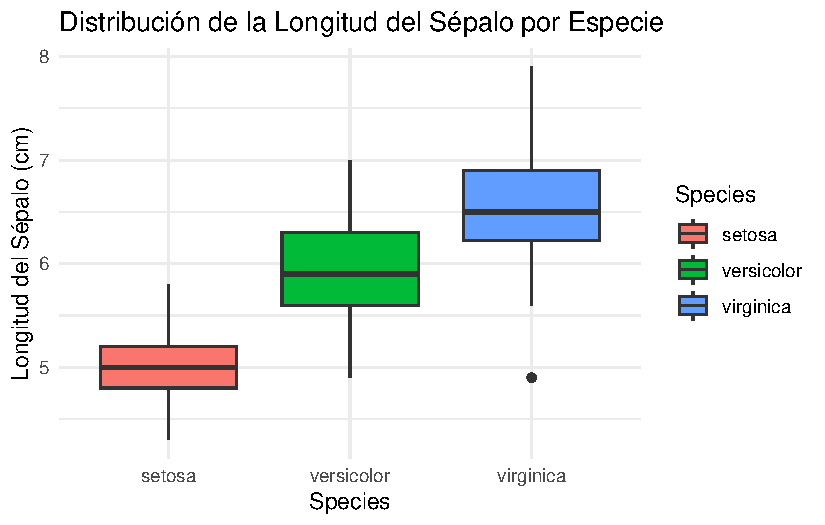
\includegraphics[keepaspectratio]{c4.3_files/figure-pdf/unnamed-chunk-17-1.pdf}}

\textbf{Interpretación:}

\begin{enumerate}
\def\labelenumi{\arabic{enumi}.}
\item
  La línea dentro de la caja representa la mediana.
\item
  Los bordes de la caja representan los cuartiles Q1 (25\%) y Q3 (75\%).
\item
  Los bigotes se extienden hasta los valores mínimo y máximo dentro de
  1.5 veces el rango intercuartílico (IQR).
\item
  Los puntos fuera de los bigotes son considerados valores atípicos.
\end{enumerate}

\subsection{Histograma}\label{histograma}

El histograma es un gráfico que muestra la distribución de frecuencia de
una variable numérica. Divide los datos en intervalos (bins) y muestra
la frecuencia de observaciones en cada intervalo.

\begin{Shaded}
\begin{Highlighting}[]
\CommentTok{\# Histograma de la longitud del sépalo}
\FunctionTok{ggplot}\NormalTok{(iris, }\FunctionTok{aes}\NormalTok{(}\AttributeTok{x =}\NormalTok{ Sepal.Length)) }\SpecialCharTok{+}
  \FunctionTok{geom\_histogram}\NormalTok{(}\AttributeTok{binwidth =} \FloatTok{0.1}\NormalTok{, }\AttributeTok{fill =} \StringTok{"steelblue"}\NormalTok{, }\AttributeTok{color =} \StringTok{"black"}\NormalTok{) }\SpecialCharTok{+}
  \FunctionTok{theme\_minimal}\NormalTok{() }\SpecialCharTok{+}
  \FunctionTok{labs}\NormalTok{(}\AttributeTok{title =} \StringTok{"Distribución de la Longitud del Sépalo"}\NormalTok{,}
       \AttributeTok{x =} \StringTok{"Longitud del Sépalo (cm)"}\NormalTok{,}
       \AttributeTok{y =} \StringTok{"Frecuencia"}\NormalTok{)}
\end{Highlighting}
\end{Shaded}

\pandocbounded{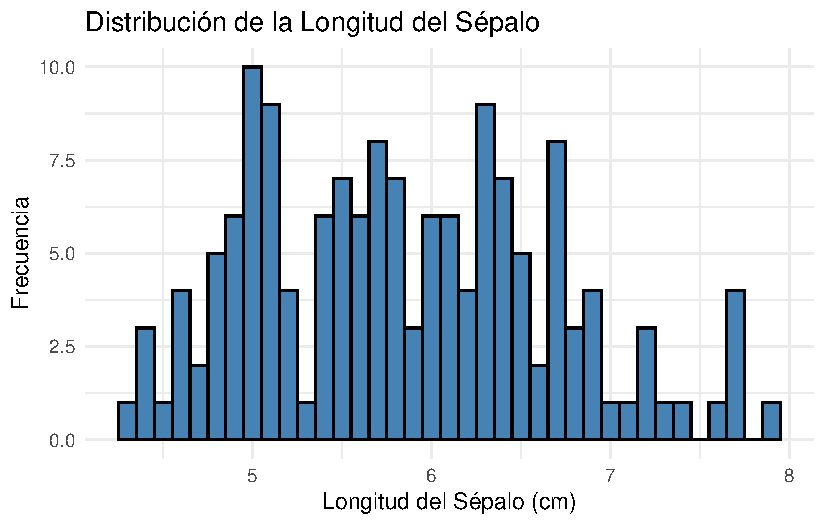
\includegraphics[keepaspectratio]{c4.3_files/figure-pdf/unnamed-chunk-18-1.pdf}}

\textbf{Interpretación:}

\begin{enumerate}
\def\labelenumi{\arabic{enumi}.}
\item
  El eje x representa los valores de la variable.
\item
  El eje y representa la frecuencia de observaciones en cada intervalo.
\item
  La forma del histograma puede indicar la simetría, asimetría y
  curtosis de la distribución.
\end{enumerate}

\subsection{Gráfico de Dispersión (Scatter
Plot)}\label{gruxe1fico-de-dispersiuxf3n-scatter-plot}

El gráfico de dispersión se utiliza para visualizar la relación entre
dos variables numéricas. Cada punto en el gráfico representa una
observación, con la posición del punto determinada por los valores de
las dos variables.

\begin{Shaded}
\begin{Highlighting}[]
\CommentTok{\# Gráfico de dispersión entre la longitud y el ancho del sépalo}
\FunctionTok{ggplot}\NormalTok{(iris, }\FunctionTok{aes}\NormalTok{(}\AttributeTok{x =}\NormalTok{ Sepal.Length, }\AttributeTok{y =}\NormalTok{ Sepal.Width, }\AttributeTok{color =}\NormalTok{ Species)) }\SpecialCharTok{+}
  \FunctionTok{geom\_point}\NormalTok{() }\SpecialCharTok{+}
  \FunctionTok{theme\_minimal}\NormalTok{() }\SpecialCharTok{+}
  \FunctionTok{labs}\NormalTok{(}\AttributeTok{title =} \StringTok{"Relación entre Longitud y Ancho del Sépalo"}\NormalTok{,}
       \AttributeTok{x =} \StringTok{"Longitud del Sépalo (cm)"}\NormalTok{,}
       \AttributeTok{y =} \StringTok{"Ancho del Sépalo (cm)"}\NormalTok{)}
\end{Highlighting}
\end{Shaded}

\pandocbounded{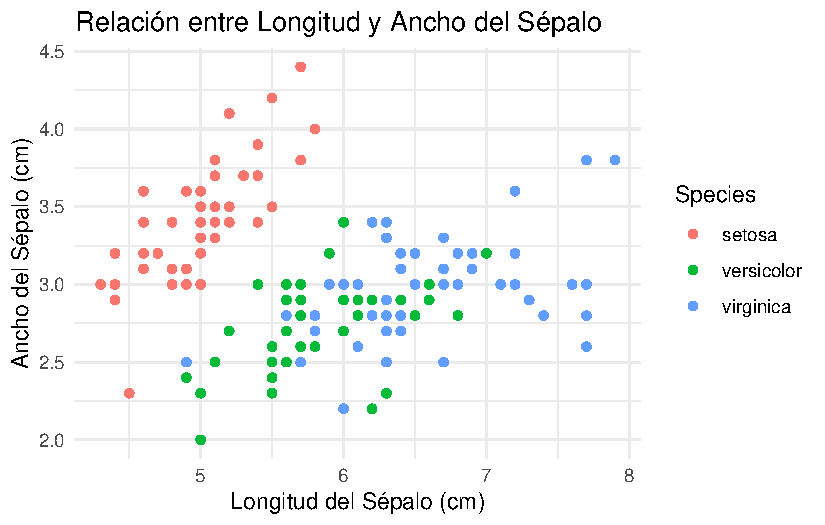
\includegraphics[keepaspectratio]{c4.3_files/figure-pdf/unnamed-chunk-19-1.pdf}}

\textbf{Interpretación:}

\begin{enumerate}
\def\labelenumi{\arabic{enumi}.}
\item
  El gráfico muestra la relación entre dos variables.
\item
  Los patrones en el gráfico pueden indicar correlación positiva,
  negativa o ninguna correlación.
\item
  Se pueden utilizar diferentes colores o formas para representar
  diferentes grupos.
\end{enumerate}

\part{5. Estadística descriptiva para datos agrupados}

\bookmarksetup{startatroot}

\chapter{Introducción y formulario}\label{introducciuxf3n-y-formulario}

El análisis de datos agrupados es una técnica que permite resumir y
describir conjuntos extensos de observaciones mediante la organización
de los valores en intervalos o clases (Lind, Marchal, \& Wathen, 2017).
Esta agrupación facilita la identificación de patrones y tendencias
generales, así como la comparación entre diferentes conjuntos de datos.
Para caracterizar la distribución de los datos agrupados, se emplean
varios tipos de medidas: las medidas de tendencia central, las medidas
de dispersión y las medidas de posición relativa (Triola, 2018).

\textbf{Aplicaciones de la estadística descriptiva para datos agrupados}

A pesar de la disponibilidad de software estadístico avanzado, el
análisis de datos agrupados sigue siendo relevante en diversas
situaciones prácticas (Anderson et al., 2018). A continuación, se
presentan algunos campos de aplicación:

\begin{enumerate}
\def\labelenumi{\arabic{enumi}.}
\item
  \textbf{Estudios epidemiológicos:} Los datos sobre la incidencia de
  enfermedades a menudo se presentan en forma de rangos de edad o
  niveles de exposición, lo que requiere el uso de técnicas de datos
  agrupados para calcular tasas y comparar poblaciones (Triola, 2018).
\item
  \textbf{Investigaciones de mercado:} Los datos sobre ingresos o gastos
  de los consumidores pueden estar disponibles solo en forma de
  intervalos, lo que exige el uso de métodos de datos agrupados para
  estimar promedios y evaluar la distribución del gasto (Lind et al.,
  2017).
\item
  \textbf{Agronomía:} Los datos sobre rendimientos de cultivos o
  características del suelo pueden estar agrupados debido a limitaciones
  en la precisión de la medición o a la necesidad de proteger la
  confidencialidad de los datos (López \& González, 2018).
\item
  \textbf{Control de calidad:} En la industria, los datos sobre las
  dimensiones de productos o el tiempo de vida útil pueden estar
  agrupados en rangos para facilitar el análisis y la toma de decisiones
  (Anderson et al., 2018).
\item
  \textbf{Análisis demográfico:} Los datos sobre la distribución de la
  población por grupos de edad y nivel socioeconómico se analizan
  mediante técnicas de datos agrupados para comprender las
  características de una población (Lind et al., 2017).
\item
  \textbf{Análisis de riesgos:} En finanzas y seguros, los datos sobre
  pérdidas o siniestros se agrupan para evaluar la probabilidad de
  eventos extremos y establecer primas o reservas adecuadas (Triola,
  2018).
\end{enumerate}

\section{Construcción de la Tabla de
Frecuencia}\label{construcciuxf3n-de-la-tabla-de-frecuencia}

Antes de calcular estas medidas, es necesario construir una tabla de
frecuencia para los datos agrupados. Este proceso implica los siguientes
pasos:

\subsection{Determinación del número de
clases}\label{determinaciuxf3n-del-nuxfamero-de-clases}

El número de clases, denotado como \(k\), se estima frecuentemente
mediante la regla de Sturges, que se expresa como:

\[\huge k = 1 + 3.322 \log_{10}(N)\]

donde \(N\) representa el número total de observaciones. Esta fórmula
proporciona una guía para seleccionar un número de clases que permita un
análisis adecuado, evitando tanto la excesiva fragmentación como la
pérdida de información relevante (Triola, 2014).

\textbf{Recomendación para la aproximación del resultado de la regla de
Sturges:} Dado que el número de clases debe ser un entero, es común
redondear el resultado de la fórmula de Sturges al entero más cercano.
Sin embargo, es importante considerar el contexto del análisis y la
naturaleza de los datos. En algunos casos, puede ser preferible
redondear hacia arriba o hacia abajo para obtener un número de clases
que facilite la interpretación y la comparación. Por ejemplo, si el
resultado de la fórmula es 6.2, se podría optar por 6 o 7 clases,
dependiendo de si se prefiere una representación más resumida o más
detallada de los datos. En general, se recomienda experimentar con
diferentes números de clases y evaluar el impacto en la claridad y la
utilidad del análisis (Anderson et al., 2018).

\subsection{Cálculo del intervalo de
clase}\label{cuxe1lculo-del-intervalo-de-clase}

El intervalo de clase, simbolizado como \(c\), corresponde a la amplitud
de cada clase y se calcula dividiendo el rango de los datos entre el
número de clases: \[\huge
c = \frac{Rango}{k}
\]

El rango se obtiene restando el valor mínimo del valor máximo del
conjunto de datos. Es recomendable ajustar el valor de \(c\) a un número
conveniente para facilitar la interpretación y la construcción de la
tabla (Lind et al., 2017).

\subsection{Definición de los límites de
clase}\label{definiciuxf3n-de-los-luxedmites-de-clase}

Cada clase se define por un límite inferior y un límite superior. Para
evitar ambigüedades en la asignación de los datos a las clases, se
utiliza una notación estándar:

\begin{enumerate}
\def\labelenumi{\arabic{enumi}.}
\item
  \textbf{Corchete {[} :} Indica que el límite está incluido en el
  intervalo.
\item
  \textbf{Paréntesis ) :} Indica que el límite no está incluido en el
  intervalo.
\end{enumerate}

Por ejemplo, el intervalo {[}10, 20) incluye todos los valores desde 10
hasta 19.999\ldots, pero no incluye el valor 20. Esta distinción es
crucial para evitar ambigüedades y asegurar que cada dato se clasifique
en un único intervalo. La correcta definición de los límites de clase
garantiza que cada observación se asigne a una única clase, evitando la
superposición y facilitando el análisis (López \& González, 2018).

\subsection{Frecuencia Absoluta}\label{frecuencia-absoluta}

La frecuencia absoluta, denotada como \(f_i\)\hspace{0pt}, representa el
número de observaciones que pertenecen a la clase \(i\). Este valor
proporciona una medida directa de la concentración de datos en cada
intervalo y es fundamental para el cálculo de las demás medidas
estadísticas (Triola, 2014).

\subsection{Frecuencia Relativa}\label{frecuencia-relativa}

La frecuencia relativa, denotada como \(fr_i\)\hspace{0pt}, se calcula
dividiendo la frecuencia absoluta de la clase \(i\) entre el número
total de observaciones \(N\):

\[\huge fr_i = \frac{f_i}{N}\]

La frecuencia relativa expresa la proporción de observaciones que
pertenecen a cada clase y permite comparar la distribución de diferentes
conjuntos de datos, independientemente de su tamaño. La suma de las
frecuencias relativas de todas las clases debe ser igual a 1 (Lind et
al., 2017).

\subsection{Frecuencia Acumulada}\label{frecuencia-acumulada}

La frecuencia acumulada, denotada como \(Fa_i\)\hspace{0pt}, representa
el número total de observaciones que son menores o iguales al límite
superior de la clase \(i\). Se calcula sumando las frecuencias absolutas
de todas las clases anteriores a la clase \(i\) y la frecuencia absoluta
de la clase \(i\): \[\huge Fa_i = \sum_{j=1}^{i} f_j\]

La frecuencia acumulada proporciona información sobre la distribución de
los datos a lo largo de todo el rango de valores y es útil para
identificar percentiles y cuartiles (Anderson et al., 2018).

\subsection{Frecuencia Relativa
Acumulada}\label{frecuencia-relativa-acumulada}

La frecuencia relativa acumulada, denotada como \(Fra_i\)\hspace{0pt},
se calcula dividiendo la frecuencia acumulada de la clase \(i\) entre el
número total de observaciones \(N\):

\[\huge Fra_i = \frac{Fa_i}{N}\]

La frecuencia relativa acumulada expresa la proporción de observaciones
que son menores o iguales al límite superior de la clase \(i\) y permite
comparar la distribución de diferentes conjuntos de datos en términos de
proporciones acumuladas. La frecuencia relativa acumulada del último
intervalo debe ser igual a 1 (Triola, 2014).

\section{Medidas de Tendencia Central para Datos
Agrupados}\label{medidas-de-tendencia-central-para-datos-agrupados}

Una vez construida la tabla de frecuencia, se procede a calcular las
medidas de tendencia central, que resumen la posición central de la
distribución de los datos. Las principales medidas de tendencia central
para datos agrupados son la media aritmética, la mediana y la moda.

\subsection{Media Aritmética}\label{media-aritmuxe9tica-2}

La media aritmética para datos agrupados, denotada como \(\bar{x}\), se
calcula como la suma ponderada de los puntos medios de cada clase, donde
los pesos son las frecuencias absolutas de cada clase:
\[\huge \bar{x} = \frac{\sum_{i=1}^{k} f_i \cdot x_i}{N}\]

donde \(f_i\)\hspace{0pt} es la frecuencia absoluta de la clase \(i\),
\(x_i\)\hspace{0pt} es el punto medio de la clase \(i\), \(k\) es el
número de clases y \(N\) es el número total de observaciones. El punto
medio de cada clase se calcula como el promedio de los límites inferior
y superior de la clase (Lind et al., 2017).

\subsection{Mediana}\label{mediana-2}

La mediana es el valor que divide la distribución de los datos en dos
partes iguales. Para calcular la mediana en datos agrupados, primero se
identifica la clase mediana, que es la primera clase cuya frecuencia
acumulada es mayor o igual a \(N/2\). Luego, se aplica la siguiente
fórmula:

\[\huge Me = L_{inf} + \frac{\frac{N}{2} - Fa_{ant}}{f_m} \cdot c\]

donde \(L_{inf}\)\hspace{0pt} es el límite inferior de la clase mediana,
\(N\) es el número total de observaciones, \(Fa_{ant}\)\hspace{0pt} es
la frecuencia acumulada de la clase anterior a la clase mediana,
\(f_m\)\hspace{0pt} es la frecuencia absoluta de la clase mediana y
\(c\) es el intervalo de clase (Triola, 2014).

\subsection{Moda}\label{moda-2}

La moda es el valor que ocurre con mayor frecuencia en la distribución
de los datos. Para calcular la moda en datos agrupados, primero se
identifica la clase modal, que es la clase con la mayor frecuencia
absoluta. Luego, se aplica la siguiente fórmula:
\[ \huge Mo = L_{inf} + \frac{d_1}{d_1 + d_2} \cdot c\]

donde \(L_{inf}\)\hspace{0pt} es el límite inferior de la clase modal,
\(d_1\)\hspace{0pt} es la diferencia entre la frecuencia de la clase
modal y la frecuencia de la clase anterior, \(d_2\)\hspace{0pt} es la
diferencia entre la frecuencia de la clase modal y la frecuencia de la
clase posterior, y \(c\) es el intervalo de clase (Anderson et al.,
2018).

\section{Medidas de Dispersión para Datos
Agrupados}\label{medidas-de-dispersiuxf3n-para-datos-agrupados}

Las medidas de dispersión cuantifican el grado de variabilidad o
dispersión de los datos respecto a las medidas de tendencia central. Las
principales medidas de dispersión para datos agrupados son el rango, la
varianza, la desviación estándar y el coeficiente de variación.

\subsection{Rango}\label{rango-2}

El rango es la medida de dispersión más simple y se calcula como la
diferencia entre el valor máximo y el valor mínimo de los datos. Para
datos agrupados, el rango se aproxima restando el límite inferior de la
primera clase al límite superior de la última clase:

\[\huge Rango = L_{sup,k} - L_{inf,1}\]

donde \(L_{sup,k}\)\hspace{0pt} es el límite superior de la última clase
y \(L_{inf,1}\) es el límite inferior de la primera clase. Aunque es
fácil de calcular, el rango es sensible a los valores extremos y no
proporciona información sobre la distribución de los datos entre los
extremos (Triola, 2014).

\subsection{Varianza}\label{varianza-2}

La varianza es una medida que cuantifica la dispersión de los datos
respecto a la media aritmética. En el caso de datos agrupados, la
varianza muestral se calcula considerando la frecuencia de cada clase y
el punto medio correspondiente. La fórmula clásica para la varianza es
la siguiente:\\
\[\huge s^2 = \frac{\sum_{i=1}^{k} f_i \cdot (x_i - \bar{x})^2}{N - 1}\]

donde \(f_i\)\hspace{0pt} es la frecuencia absoluta de la clase \(i\),
\(x_i\)\hspace{0pt} es el punto medio de la clase \(i\), \(\bar{x}\) es
la media aritmética y \(N\) es el número total de observaciones. La
varianza proporciona una medida de la dispersión de los datos alrededor
de la media, pero se expresa en unidades al cuadrado, lo que dificulta
su interpretación directa (Lind et al., 2017).

Como alternativa, la varianza también puede calcularse utilizando una
fórmula operativa, que resulta especialmente útil cuando se dispone de
la suma de los productos de las frecuencias por los puntos medios y sus
cuadrados. Esta fórmula es algebraicamente equivalente a la anterior y
se expresa así:

\[ \LARGE s^2 = \frac{\sum_{i=1}^{k} f_i x_i^2 - \frac{\left(\sum_{i=1}^{k} f_i x_i\right)^2}{N}}{N - 1}\]

donde \(f_i\)\hspace{0pt} es la frecuencia absoluta de la clase \(i\),
\(x_i\)\hspace{0pt} es el punto medio de la clase \(i\), \(N\) es el
número total de observaciones y kkk es el número de clases. En esta
fórmula, \(\sum_{i=1}^{k} f_i x_i^2\) representa la suma de los
productos de la frecuencia por el cuadrado del punto medio de cada
clase, mientras que \(\sum_{i=1}^{k} f_i x_i\) corresponde a la suma de
los productos de la frecuencia por el punto medio de cada clase.

Ambas fórmulas, la clásica y la operativa, son equivalentes y
proporcionan el mismo resultado si se aplican correctamente (Lind et
al., 2017; López \& González, 2018; Triola, 2018).

\subsection{Desviación Estándar}\label{desviaciuxf3n-estuxe1ndar-2}

La desviación estándar es la raíz cuadrada de la varianza y se expresa
en las mismas unidades que los datos originales. Para datos agrupados,
la desviación estándar se calcula como: \[\huge s = \sqrt{s^2}\]

La desviación estándar proporciona una medida de la dispersión de los
datos alrededor de la media y es más fácil de interpretar que la
varianza. Un valor alto de la desviación estándar indica una mayor
dispersión de los datos, mientras que un valor bajo indica una menor
dispersión (Anderson et al., 2018).

\subsection{Coeficiente de
Variación}\label{coeficiente-de-variaciuxf3n-2}

El coeficiente de variación es una medida relativa de dispersión que se
calcula dividiendo la desviación estándar entre la media aritmética:
\[ \huge CV = \frac{s}{\bar{x}} \cdot 100\%\]

El coeficiente de variación expresa la dispersión de los datos como un
porcentaje de la media y permite comparar la variabilidad de diferentes
conjuntos de datos, independientemente de sus unidades de medida. Un
valor alto del coeficiente de variación indica una mayor variabilidad
relativa, mientras que un valor bajo indica una menor variabilidad
relativa (Triola, 2014).

\section{Medidas de Posición Relativa para Datos
Agrupados}\label{medidas-de-posiciuxf3n-relativa-para-datos-agrupados}

Las medidas de posición relativa describen la ubicación de un valor
específico en relación con el resto de los datos. Las principales
medidas de posición relativa son los cuartiles y los percentiles.

\subsection{Cuartiles}\label{cuartiles-2}

Los cuartiles dividen la distribución de los datos en cuatro partes
iguales, cada una conteniendo el 25\% de las observaciones. Los tres
cuartiles se denotan como \(Q_1\)\hspace{0pt}, \(Q_2\)\hspace{0pt} y
\(Q_3\)\hspace{0pt}.

\begin{enumerate}
\def\labelenumi{\arabic{enumi}.}
\item
  \(Q_1\)\hspace{0pt} (Primer Cuartil): Es el valor que separa el 25\%
  inferior de los datos del 75\% superior.
\item
  \(Q_2\)\hspace{0pt} (Segundo Cuartil): Es el valor que coincide con la
  mediana y separa el 50\% inferior de los datos del 50\% superior.
\item
  \(Q_3\)\hspace{0pt} (Tercer Cuartil): Es el valor que separa el 75\%
  inferior de los datos del 25\% superior.
\end{enumerate}

Para calcular los cuartiles en datos agrupados, primero se identifica la
clase cuartil, que es la primera clase cuya frecuencia acumulada es
mayor o igual a \(i \cdot N/4\), donde \(i\) es el número del cuartil
(1, 2 o 3). Luego, se aplica la siguiente fórmula:
\[\huge Q_i = L_{inf} + \frac{\frac{i \cdot N}{4} - Fa_{ant}}{f_q} \cdot c\]

donde \(L_{inf}\)\hspace{0pt} es el límite inferior de la clase cuartil,
\(N\) es el número total de observaciones, \(Fa_{ant}\)\hspace{0pt} es
la frecuencia acumulada de la clase anterior a la clase cuartil,
\(f_q\)\hspace{0pt} es la frecuencia absoluta de la clase cuartil y
\(c\) es el intervalo de clase (Lind et al., 2017).

\subsection{Percentiles}\label{percentiles-2}

Los percentiles dividen la distribución de los datos en cien partes
iguales, cada una conteniendo el 1\% de las observaciones. El percentil
\(P_p\)\hspace{0pt} es el valor que separa el \(p \%\) inferior de los
datos del \((100−p) \%\) superior.

Para calcular los percentiles en datos agrupados, primero se identifica
la clase percentil, que es la primera clase cuya frecuencia acumulada es
mayor o igual a \(p \cdot N/100\). Luego, se aplica la siguiente
fórmula:
\[\LARGE P_p = L_{inf} + \frac{\frac{p \cdot N}{100} - Fa_{ant}}{f_p} \cdot c\]

donde \(L_{inf}\)\hspace{0pt} es el límite inferior de la clase
percentil, \(N\) es el número total de observaciones,
\(Fa_{ant}\)\hspace{0pt} es la frecuencia acumulada de la clase anterior
a la clase percentil, \(f_p\)\hspace{0pt} es la frecuencia absoluta de
la clase percentil y \(c\) es el intervalo de clase (Triola, 2014).

\bookmarksetup{startatroot}

\chapter{Ejemplo empleando el
formulario}\label{ejemplo-empleando-el-formulario}

\section{Base de datos}\label{base-de-datos-1}

\textbf{Referencia del dataset:} Fisher, R. (1936). Iris {[}Dataset{]}.
UCI Machine Learning Repository. \url{https://doi.org/10.24432/C56C76}

\textbf{Acceso a recursos:} El script completo con el ejemplo
desarrollado y la base de datos IRIS pueden descargarse en el siguiente
repositorio:

A continuación, se presenta un conjunto de datos correspondientes a la
longitud del pétalo (en cm) de 150 flores de la especie \emph{Iris},
organizados en formato matricial para facilitar su visualización y
análisis. Estos datos serán utilizados para ilustrar el cálculo de
estadísticos descriptivos para datos agrupados, siguiendo las
metodologías propuestas en la sección aterior.

\begin{longtable}[]{@{}llllllllll@{}}
\toprule\noalign{}
\endhead
\bottomrule\noalign{}
\endlastfoot
1.4 & 1.4 & 1.3 & 1.5 & 1.4 & 1.7 & 1.4 & 1.5 & 1.4 & 1.5 \\
1.5 & 1.6 & 1.4 & 1.1 & 1.2 & 1.5 & 1.3 & 1.4 & 1.7 & 1.5 \\
1.7 & 1.5 & 1.0 & 1.7 & 1.9 & 1.6 & 1.6 & 1.5 & 1.4 & 1.6 \\
1.6 & 1.5 & 1.5 & 1.4 & 1.5 & 1.2 & 1.3 & 1.4 & 1.3 & 1.5 \\
1.3 & 1.3 & 1.3 & 1.6 & 1.9 & 1.4 & 1.6 & 1.4 & 1.5 & 1.4 \\
4.7 & 4.5 & 4.9 & 4.0 & 4.6 & 4.5 & 4.7 & 3.3 & 4.6 & 3.9 \\
3.5 & 4.2 & 4.0 & 4.7 & 3.6 & 4.4 & 4.5 & 4.1 & 4.5 & 3.9 \\
4.8 & 4.0 & 4.9 & 4.7 & 4.3 & 4.4 & 4.8 & 5.0 & 4.5 & 3.5 \\
3.8 & 3.7 & 3.9 & 5.1 & 4.5 & 4.5 & 4.7 & 4.4 & 4.1 & 4.0 \\
4.4 & 4.6 & 4.0 & 3.3 & 4.2 & 4.2 & 4.2 & 4.3 & 3.0 & 4.1 \\
6.0 & 5.1 & 5.9 & 5.6 & 5.8 & 6.6 & 4.5 & 6.3 & 5.8 & 6.1 \\
5.1 & 5.3 & 5.5 & 5.0 & 5.1 & 5.3 & 5.5 & 6.7 & 6.9 & 5.0 \\
5.7 & 4.9 & 6.7 & 4.9 & 5.7 & 6.0 & 4.8 & 4.9 & 5.6 & 5.8 \\
6.1 & 6.4 & 5.6 & 5.1 & 5.6 & 6.1 & 5.6 & 5.5 & 4.8 & 5.4 \\
5.6 & 5.1 & 5.1 & 5.9 & 5.7 & 5.2 & 5.0 & 5.2 & 5.4 & 5.1 \\
\end{longtable}

\section{Construcción de la Tabla de
Frecuencias}\label{construcciuxf3n-de-la-tabla-de-frecuencias}

\subsection{Determinación del rango
(R)}\label{determinaciuxf3n-del-rango-r}

El rango es la diferencia entre el valor máximo y el valor mínimo de la
variable:

\[\huge R = X_{\text{max}} - X_{\text{min}}\] Para la longitud de
pétalo: \[\huge R = 6.9 - 1.0 = 5.9\]

\subsection{Cálculo del número de clases
(K)}\label{cuxe1lculo-del-nuxfamero-de-clases-k}

El número de clases se determina con la Regla de Sturges:
\[\huge k = 1 + 3.322 \log_{10} N\] Donde \(n\) es el número total de
datos:
\[\LARGE k = 1 + 3.322 \log_{10} 150 \approx 1 + 3.322 \times 2.1761 \approx 8.22\]
Se redondea al entero más cercano:

\[\Huge k = 8\]

\subsection{Cálculo de la amplitud de clase
(C)}\label{cuxe1lculo-de-la-amplitud-de-clase-c}

La amplitud de clase se calcula así: \[\Huge C = \frac{R}{k}\]
Sustituyendo valores: \[\Huge C = \frac{5.9}{8} = 0.7375 \approx 0.75\]

\subsection{Determinación de los límites de
clase}\label{determinaciuxf3n-de-los-luxedmites-de-clase}

El primer límite inferior es el valor mínimo (\(1.0\)). Los siguientes
se obtienen sumando la amplitud de clase (\(C\)).\\
Para evitar que un valor pertenezca a dos clases al mismo tiempo, se
utiliza la notación de intervalos semiabiertos:

\begin{enumerate}
\def\labelenumi{\arabic{enumi}.}
\item
  El corchete \([\) indica que el límite inferior está incluido en la
  clase.
\item
  El paréntesis \()\) indica que el límite superior no está incluido en
  la clase.
\end{enumerate}

Por ejemplo, el primer intervalo se escribe:

\[\LARGE [1.00, 1.75)\]

Esto significa que la clase incluye todos los valores \(x\) tales que
\(1.00≤x<1.75\).

Los intervalos de clase quedan así: \[\large \begin{aligned}
\text{Clase 1:} & \quad [1.00, 1.75) \\
\text{Clase 2:} & \quad [1.75, 2.50) \\
\text{Clase 3:} & \quad [2.50, 3.25) \\
\text{Clase 4:} & \quad [3.25, 4.00) \\
\text{Clase 5:} & \quad [4.00, 4.75) \\
\text{Clase 6:} & \quad [4.75, 5.50) \\
\text{Clase 7:} & \quad [5.50, 6.25) \\
\text{Clase 8:} & \quad [6.25, 7.00] \\
\end{aligned}\]

\textbf{Nótese} que en la última clase se utiliza el corchete de cierre
\(]\) para incluir el valor máximo.

\subsection{Cálculo de la marca de
clase}\label{cuxe1lculo-de-la-marca-de-clase}

La marca de clase es el punto medio de cada intervalo:
\[\huge x_i = \frac{L_i + L_s}{2}\] Por ejemplo, para la primera clase:
\[ \huge x_1 = \frac{1.00 + 1.75}{2} = 1.375\]

\subsection{Cálculo de la frecuencia
absoluta}\label{cuxe1lculo-de-la-frecuencia-absoluta}

La frecuencia absoluta es el número de datos en cada clase, obtenida por
conteo directo.

\subsection{Cálculo de la frecuencia
relativa}\label{cuxe1lculo-de-la-frecuencia-relativa}

La frecuencia relativa se calcula así: \[\huge fr_i = \frac{f_i}{N}\]

Por ejemplo, para la primera clase:
\[\huge fr_i = \frac{48}{150} = 0.32\]

\subsection{Cálculo de la frecuencia
acumulada}\label{cuxe1lculo-de-la-frecuencia-acumulada}

La frecuencia acumulada es la suma de las frecuencias absolutas hasta la
clase \(i\): \[\huge fa_i = \sum_{j=1}^{i} f_j\]

Por ejemplo, para la cuarta clase:
\[ \Large fa_4 = f_1 + f_2 + f_3 + f_4 = 48 + 0 + 0 + 15 = 63\]

\subsection{\texorpdfstring{Cálculo de \(f_i x_i\)\hspace{0pt} y
\(f_i x_i^2\)}{Cálculo de f\_i x\_i\hspace{0pt} y f\_i x\_i\^{}2}}\label{cuxe1lculo-de-f_i-x_i-y-f_i-x_i2}

Estos productos se utilizan para cálculos posteriores:
\[\huge f_i x_i = f_i \times x_i\]
\[\huge f_i x_i^2 = f_i \times (x_i)^2\] Por ejemplo, para la primera
clase: \[\LARGE f_1 x_1 = 48 \times 1.375 = 66.00\]
\[\LARGE f_1 x_1^2 = 48 \times (1.375)^2 = 48 \times 1.890625 = 90.75\]

\section{Tabla de frecuencia}\label{tabla-de-frecuencia}

\begin{longtable}[]{@{}
  >{\raggedright\arraybackslash}p{(\linewidth - 16\tabcolsep) * \real{0.1111}}
  >{\raggedright\arraybackslash}p{(\linewidth - 16\tabcolsep) * \real{0.1111}}
  >{\raggedright\arraybackslash}p{(\linewidth - 16\tabcolsep) * \real{0.1111}}
  >{\raggedright\arraybackslash}p{(\linewidth - 16\tabcolsep) * \real{0.1111}}
  >{\raggedright\arraybackslash}p{(\linewidth - 16\tabcolsep) * \real{0.1111}}
  >{\raggedright\arraybackslash}p{(\linewidth - 16\tabcolsep) * \real{0.1111}}
  >{\raggedright\arraybackslash}p{(\linewidth - 16\tabcolsep) * \real{0.1111}}
  >{\raggedright\arraybackslash}p{(\linewidth - 16\tabcolsep) * \real{0.1111}}
  >{\raggedright\arraybackslash}p{(\linewidth - 16\tabcolsep) * \real{0.1111}}@{}}
\toprule\noalign{}
\begin{minipage}[b]{\linewidth}\raggedright
Clase
\end{minipage} & \begin{minipage}[b]{\linewidth}\raggedright
Límite Inferior (LI)
\end{minipage} & \begin{minipage}[b]{\linewidth}\raggedright
Límite Superior (LS)
\end{minipage} & \begin{minipage}[b]{\linewidth}\raggedright
Marca de clase (\(x_i\))
\end{minipage} & \begin{minipage}[b]{\linewidth}\raggedright
Frecuencia ( \(f_i\) \hspace{0pt})
\end{minipage} & \begin{minipage}[b]{\linewidth}\raggedright
Frecuencia relativa (\(fr_i\)\hspace{0pt})
\end{minipage} & \begin{minipage}[b]{\linewidth}\raggedright
Frecuencia acumulada (\(fa_i\))
\end{minipage} & \begin{minipage}[b]{\linewidth}\raggedright
\(f_i x_i\)
\end{minipage} & \begin{minipage}[b]{\linewidth}\raggedright
\(f_i x_i^2\)
\end{minipage} \\
\midrule\noalign{}
\endhead
\bottomrule\noalign{}
\endlastfoot
1 & 1.000 & 1.750 & 1.375 & 48 & 0.320 & 48 & 66.000 & 90.750 \\
2 & 1.750 & 2.500 & 2.125 & 2 & 0.013 & 50 & 4.250 & 9.031 \\
3 & 2.500 & 3.250 & 2.875 & 1 & 0.007 & 51 & 2.875 & 8.266 \\
4 & 3.250 & 4.000 & 3.625 & 10 & 0.067 & 61 & 36.250 & 131.406 \\
5 & 4.000 & 4.750 & 4.375 & 34 & 0.227 & 95 & 148.750 & 650.781 \\
6 & 4.750 & 5.500 & 5.125 & 27 & 0.180 & 122 & 138.375 & 709.172 \\
7 & 5.500 & 6.250 & 5.875 & 22 & 0.147 & 144 & 129.250 & 759.344 \\
8 & 6.250 & 7.000 & 6.625 & 6 & 0.040 & 150 & 39.750 & 263.344 \\
Total & & & & 150 & 1.000 & & 565.500 & 2622.094 \\
\end{longtable}

\section{Medidas de tendencia
central}\label{medidas-de-tendencia-central-2}

Una vez construida la tabla de frecuencia, se procede a calcular las
medidas de tendencia central, que resumen la posición central de la
distribución de los datos.

\subsection{Media Aritmética}\label{media-aritmuxe9tica-3}

La formula para calcular la media aritmpetica es la siguiente:

\[\huge \bar{x} = \frac{\sum_{i=1}^{k} f_i \cdot x_i}{N}\]

Sustituyendo valores

\[\huge \bar{x} = \frac{565.50}{150}=3.77\]

\subsection{Mediana}\label{mediana-3}

Para el calculo de la mediana hay que identificar la primera clase donde
la frecuencia acumulada \(fa_i\) supera \(N/2\). Para este ejemplo
\(N/2\) al sustituir valores equivale a \(150/2=75\) siendo la clase
numero 5 aquella donde la frecuencia acumulada supera \(N/2\) siendo la
formula para el cálculo de la mediana la siguiente:\\
\[\huge Me = L_{inf} + \frac{\frac{N}{2} - Fa_{ant}}{f_m} \cdot c\]
Sustituyendo valores
\[\huge Me = 4.00 + \frac{\frac{150}{2} - 61}{34} \cdot 0.75=4.31\]

\subsection{Moda}\label{moda-3}

Para el calculo de la moda hay que identificar clase con mayor
frecuencia absoluta siendo la clase numero 1 para este ejemplo. Siendo
la formula para el cálculo de la moda la siguiente:

\[ \huge Mo = L_{inf} + \frac{d_1}{d_1 + d_2} \cdot c\]

Sustituyendo valores:

\[ \LARGE Mo = 1.00 + \frac{(48-0)}{(48-0) + (48-2)} \cdot 0.75=1.383\]

\section{Medidas de dispersión}\label{medidas-de-dispersiuxf3n-2}

\subsection{Rango}\label{rango-3}

El rango se aproxima restando el límite inferior de la primera clase al
límite superior de la última clase siendo su formula la siguiente:

\[\huge Rango = L_{sup,k} - L_{inf,1}\]

Sustituyendo valores:

\[\huge Rango = 7.00 - 1.00=6.00\]

\subsection{Varianza}\label{varianza-3}

Para el calculo de la varianza se utilizará la siguiente formula
operativa, que resulta especialmente útil porque se dispone de la suma
de los productos de las frecuencias por los puntos medios y sus
cuadrados.

\[ \LARGE s^2 = \frac{\sum_{i=1}^{k} f_i x_i^2 - \frac{\left(\sum_{i=1}^{k} f_i x_i\right)^2}{N}}{N - 1}\]

Sustituyendo valores:

\[ \LARGE s^2 = \frac{2622.094 - \frac{\left(565.500\right)^2}{150}}{150 - 1}=3.29\]

\subsection{Desviación Estándar}\label{desviaciuxf3n-estuxe1ndar-3}

La desviación estándar es la raíz cuadrada de la varianza y se expresa
en las mismas unidades que los datos originales. Para datos agrupados,
la desviación estándar se calcula como:

\[\huge s = \sqrt{s^2}\]

Sustituyendo valores

\[\huge s = \sqrt{3.29}=1.645\]

\subsection{Coeficiente de
Variación}\label{coeficiente-de-variaciuxf3n-3}

El coeficiente de variación es una medida relativa de dispersión que se
calcula dividiendo la desviación estándar entre la media aritmética:
\[ \huge CV = \frac{s}{\bar{x}} \cdot 100\%\]

Sustituyendo valores:

\[ \huge CV = \frac{1.645}{3.77} \cdot 100\%=43.63\%\]

\section{Medidas de posición
relativa}\label{medidas-de-posiciuxf3n-relativa-2}

\subsection{Cuartiles}\label{cuartiles-3}

Para calcular los cuartiles en datos agrupados, primero se identifica la
clase cuartil, que es la primera clase cuya frecuencia acumulada es
mayor o igual a~\(i⋅N/4\), donde \(i\) es el número del cuartil (1, 2 o
3). Luego, se aplica la siguiente fórmula:

\[\huge Q_i = L_{inf} + \frac{\frac{i \cdot N}{4} - Fa_{ant}}{f_q} \cdot c\]

Para el ejemplo se calculará el cuartil 1 (Q1) por lo que primero se
identifica la clase dentro de la que se encuentra, para ello se usa la
formula \(i⋅N/4\), sustituyendo valores esto sería \(1\cdot 150/4=38.5\)
siendo la clase donde la frecuencia acumulada supera este valor por
primera vez la clase 1, ya con esta información se procede a sustituir
valores en la fórmula.

\[\huge Q_1 = 1.0 + \frac{\frac{1 \cdot 150}{4} - 0}{48} \cdot 0.75=1.59\]

\subsection{Percentiles}\label{percentiles-3}

Para calcular los percentiles en datos agrupados, primero se identifica
la clase percentil, que es la primera clase cuya frecuencia acumulada es
mayor o igual a \(p \cdot N/100\). Luego, se aplica la siguiente
fórmula:

\[\huge P_p = L_{inf} + \frac{\frac{p \cdot N}{100} - Fa_{ant}}{f_p} \cdot c\]

Para el ejemplo se calculará el percentil 80 (\(p=80\)) para ello
primero se identifica la clase a la que pertenece este percentil usando
la formula \(p \cdot N/100\) la cual al sustituir los valores equivale
a: \(80 \cdot 150/100= 120\) con este dato se ubica la clase 6 como la
clase donde se encuentra el percentil 80 al ser la primera donde la
frecuencia acumulada supera 120. Una vez obtenida esta información se
procede a sustituir valores en la formula:

\[\huge P_{80} = 4.75 + \frac {120 - 95}{27} \cdot 0.75=5.44\]

\section{Interpretación de
Resultados}\label{interpretaciuxf3n-de-resultados}

\subsection{Media aritmética}\label{media-aritmuxe9tica-4}

La media aritmética obtenida fue de 3.77 cm. Esto indica que, en
promedio, la longitud del pétalo de las flores analizadas es de 3.77
centímetros. Esta medida representa el valor central alrededor del cual
tienden a agruparse los datos y es útil para describir el comportamiento
general de la variable en estudio (López \& González, 2018).

\subsection{Mediana}\label{mediana-4}

La mediana calculada fue de 4.31 cm. Esto significa que el 50\% de las
flores tiene una longitud de pétalo menor o igual a 4.31 cm, mientras
que el otro 50\% tiene una longitud mayor o igual a este valor. La
mediana es especialmente útil cuando la distribución de los datos es
asimétrica o presenta valores extremos, ya que no se ve afectada por
estos (López \& González, 2018).

\subsection{Moda}\label{moda-4}

La moda resultó ser 1.375 cm, correspondiente a la clase con mayor
frecuencia absoluta. Esto indica que la longitud de pétalo más común
entre las flores analizadas se encuentra en el intervalo de 1.00 a 1.75
cm. La moda es relevante para identificar el valor o rango de valores
que se presentan con mayor frecuencia en el conjunto de datos (López \&
González, 2018).

\subsection{Rango}\label{rango-4}

El rango calculado fue de 6.00 cm, lo que representa la diferencia entre
la longitud máxima y mínima de los pétalos observados. Este valor
proporciona una idea general de la dispersión de los datos, mostrando el
intervalo total en el que se distribuyen las observaciones (López \&
González, 2018).

\subsection{Varianza y desviación
estándar}\label{varianza-y-desviaciuxf3n-estuxe1ndar}

La varianza obtenida fue de 3.67 cm² y la desviación estándar fue de
1.83 cm. Estos valores indican que, en promedio, las longitudes de los
pétalos se desvían 1.83 cm respecto a la media. Una desviación estándar
relativamente alta, como en este caso, sugiere que existe una
considerable variabilidad en la longitud de los pétalos dentro del grupo
analizado (López \& González, 2018).

\subsection{Coeficiente de
variación}\label{coeficiente-de-variaciuxf3n-4}

El coeficiente de variación fue de 46.88\%. Este valor, al ser mayor al
30\%, indica que la dispersión relativa de los datos respecto a la media
es alta. En términos prácticos, esto significa que la longitud de los
pétalos presenta una considerable heterogeneidad dentro del conjunto de
flores estudiadas (López \& González, 2018).

\subsection{Cuartil 1 (Q1)}\label{cuartil-1-q1}

El primer cuartil (Q1) se ubicó en 1.59 cm. Esto implica que el 25\% de
las flores tiene una longitud de pétalo menor o igual a 1.59 cm. El
análisis de los cuartiles permite identificar la distribución de los
datos en segmentos y facilita la detección de posibles asimetrías o
concentraciones de valores (López \& González, 2018).

\subsection{Percentil 80 (P80)}\label{percentil-80-p80}

El percentil 80 se calculó en 5.78 cm, lo que significa que el 80\% de
las flores tiene una longitud de pétalo menor o igual a 5.78 cm. El
percentil 80 es útil para identificar valores altos dentro de la
distribución y para realizar comparaciones entre diferentes grupos o
tratamientos (López \& González, 2018).

\bookmarksetup{startatroot}

\chapter{Ejemplo en R}\label{ejemplo-en-r}

\section{Base de datos}\label{base-de-datos-2}

\textbf{Referencia del dataset:} Fisher, R. (1936). Iris {[}Dataset{]}.
UCI Machine Learning Repository. \url{https://doi.org/10.24432/C56C76}

\textbf{Acceso a recursos:} El script completo con el ejemplo
desarrollado y la base de datos IRIS pueden descargarse en el siguiente
repositorio: \url{https://github.com/Ludwing-MJ/MTCDPR_datos_agrupados}

A continuación, se presenta un conjunto de datos correspondientes a la
longitud del pétalo (en cm) de 150 flores de la especie \emph{Iris},
organizados en formato matricial para facilitar su visualización y
análisis. Estos datos serán utilizados para ilustrar el cálculo de
estadísticos descriptivos para datos agrupados, siguiendo las
metodologías propuestas en la sección aterior.

\begin{longtable}[]{@{}llllllllll@{}}
\toprule\noalign{}
\endhead
\bottomrule\noalign{}
\endlastfoot
1.4 & 1.4 & 1.3 & 1.5 & 1.4 & 1.7 & 1.4 & 1.5 & 1.4 & 1.5 \\
1.5 & 1.6 & 1.4 & 1.1 & 1.2 & 1.5 & 1.3 & 1.4 & 1.7 & 1.5 \\
1.7 & 1.5 & 1.0 & 1.7 & 1.9 & 1.6 & 1.6 & 1.5 & 1.4 & 1.6 \\
1.6 & 1.5 & 1.5 & 1.4 & 1.5 & 1.2 & 1.3 & 1.4 & 1.3 & 1.5 \\
1.3 & 1.3 & 1.3 & 1.6 & 1.9 & 1.4 & 1.6 & 1.4 & 1.5 & 1.4 \\
4.7 & 4.5 & 4.9 & 4.0 & 4.6 & 4.5 & 4.7 & 3.3 & 4.6 & 3.9 \\
3.5 & 4.2 & 4.0 & 4.7 & 3.6 & 4.4 & 4.5 & 4.1 & 4.5 & 3.9 \\
4.8 & 4.0 & 4.9 & 4.7 & 4.3 & 4.4 & 4.8 & 5.0 & 4.5 & 3.5 \\
3.8 & 3.7 & 3.9 & 5.1 & 4.5 & 4.5 & 4.7 & 4.4 & 4.1 & 4.0 \\
4.4 & 4.6 & 4.0 & 3.3 & 4.2 & 4.2 & 4.2 & 4.3 & 3.0 & 4.1 \\
6.0 & 5.1 & 5.9 & 5.6 & 5.8 & 6.6 & 4.5 & 6.3 & 5.8 & 6.1 \\
5.1 & 5.3 & 5.5 & 5.0 & 5.1 & 5.3 & 5.5 & 6.7 & 6.9 & 5.0 \\
5.7 & 4.9 & 6.7 & 4.9 & 5.7 & 6.0 & 4.8 & 4.9 & 5.6 & 5.8 \\
6.1 & 6.4 & 5.6 & 5.1 & 5.6 & 6.1 & 5.6 & 5.5 & 4.8 & 5.4 \\
5.6 & 5.1 & 5.1 & 5.9 & 5.7 & 5.2 & 5.0 & 5.2 & 5.4 & 5.1 \\
\end{longtable}

\section{Preparación del entorno de
trabajo}\label{preparaciuxf3n-del-entorno-de-trabajo}

\begin{Shaded}
\begin{Highlighting}[]
\CommentTok{\# Instalación y carga de paquetes necesarios}
\DocumentationTok{\#\# Para manipulación y visualización de datos}
\ControlFlowTok{if}\NormalTok{ (}\SpecialCharTok{!}\FunctionTok{require}\NormalTok{(tidyverse)) }\FunctionTok{install.packages}\NormalTok{(}\StringTok{"tidyverse"}\NormalTok{)}
\DocumentationTok{\#\# Para exportar archivos en excel}
\ControlFlowTok{if}\NormalTok{ (}\SpecialCharTok{!}\FunctionTok{require}\NormalTok{(writexl)) }\FunctionTok{install.packages}\NormalTok{(}\StringTok{"writexl"}\NormalTok{)}
\DocumentationTok{\#\# Para importar archivos en excel}
\ControlFlowTok{if}\NormalTok{ (}\SpecialCharTok{!}\FunctionTok{require}\NormalTok{(readxl)) }\FunctionTok{install.packages}\NormalTok{(}\StringTok{"readxl"}\NormalTok{)}
\end{Highlighting}
\end{Shaded}

\section{Carga y Preparación de
Datos}\label{carga-y-preparaciuxf3n-de-datos}

Primero, se carga el conjunto de datos iris y se extrae la variable de
interés, en este caso, la longitud del pétalo.

\begin{Shaded}
\begin{Highlighting}[]
\CommentTok{\# Cargar el dataset iris}
\FunctionTok{data}\NormalTok{(iris)}

\CommentTok{\# Extraer la variable longitud de pétalo}
\NormalTok{longitud\_petalo }\OtherTok{\textless{}{-}}\NormalTok{ iris}\SpecialCharTok{$}\NormalTok{Petal.Length}
\end{Highlighting}
\end{Shaded}

\section{Determinación de parámetros básicos para la
agrupación}\label{determinaciuxf3n-de-paruxe1metros-buxe1sicos-para-la-agrupaciuxf3n}

Se define una función personalizada para calcular los parámetros
necesarios para agrupar los datos: número de observaciones, valores
mínimo y máximo, rango, número de clases (usando la regla de Sturges) y
amplitud de clase.

\begin{Shaded}
\begin{Highlighting}[]
\CommentTok{\# Función para calcular parámetros de agrupamiento}
\NormalTok{calcular\_parametros\_agrupamiento }\OtherTok{\textless{}{-}} \ControlFlowTok{function}\NormalTok{(datos) \{}
\NormalTok{  n }\OtherTok{\textless{}{-}} \FunctionTok{length}\NormalTok{(datos)}
\NormalTok{  x\_min }\OtherTok{\textless{}{-}} \FunctionTok{min}\NormalTok{(datos)}
\NormalTok{  x\_max }\OtherTok{\textless{}{-}} \FunctionTok{max}\NormalTok{(datos)}
\NormalTok{  rango }\OtherTok{\textless{}{-}}\NormalTok{ x\_max }\SpecialCharTok{{-}}\NormalTok{ x\_min}
  
  \CommentTok{\# Regla de Sturges para número de clases}
\NormalTok{  k }\OtherTok{\textless{}{-}} \FunctionTok{round}\NormalTok{(}\DecValTok{1} \SpecialCharTok{+} \FloatTok{3.322} \SpecialCharTok{*} \FunctionTok{log10}\NormalTok{(n))}
  
  \CommentTok{\# Amplitud de clase}
\NormalTok{  amplitud }\OtherTok{\textless{}{-}}\NormalTok{ rango }\SpecialCharTok{/}\NormalTok{ k}
  
  \FunctionTok{return}\NormalTok{(}\FunctionTok{list}\NormalTok{(}
    \AttributeTok{n =}\NormalTok{ n,}
    \AttributeTok{x\_min =}\NormalTok{ x\_min,}
    \AttributeTok{x\_max =}\NormalTok{ x\_max,}
    \AttributeTok{rango =}\NormalTok{ rango,}
    \AttributeTok{k =}\NormalTok{ k,}
    \AttributeTok{amplitud =}\NormalTok{ amplitud}
\NormalTok{  ))}
\NormalTok{\}}
\end{Highlighting}
\end{Shaded}

Una vez ya definida la función para calcular los parametros necesarios
para la agrupación de los datos (tarea que se realiza la cada vez que se
abre el software y se desea cargar la función en el entorno de trabajo).
Se procede a calcularlos:

\begin{Shaded}
\begin{Highlighting}[]
\CommentTok{\# Aplicar función}
\NormalTok{parametros }\OtherTok{\textless{}{-}} \FunctionTok{calcular\_parametros\_agrupamiento}\NormalTok{(longitud\_petalo)}
\CommentTok{\# Visualizar el resultado}
\NormalTok{parametros}
\end{Highlighting}
\end{Shaded}

\begin{verbatim}
$n
[1] 150

$x_min
[1] 1

$x_max
[1] 6.9

$rango
[1] 5.9

$k
[1] 8

$amplitud
[1] 0.7375
\end{verbatim}

\section{Construcción de la tabla de
frecuencias}\label{construcciuxf3n-de-la-tabla-de-frecuencias-1}

Se utiliza una función personalizada para construir la tabla de
frecuencias, calculando los límites de clase, marcas de clase,
frecuencias absolutas, relativas y acumuladas, así como sumas necesarias
para los cálculos posteriores.

\begin{Shaded}
\begin{Highlighting}[]
\CommentTok{\# Función corregida para construir tabla de frecuencias}
\NormalTok{construir\_tabla\_frecuencias }\OtherTok{\textless{}{-}} \ControlFlowTok{function}\NormalTok{(datos, parametros) \{}
  
  \CommentTok{\# Crear breaks (puntos de corte) para las clases}
  \CommentTok{\# Esto garantiza exactamente k clases}
\NormalTok{  breaks }\OtherTok{\textless{}{-}} \FunctionTok{seq}\NormalTok{(parametros}\SpecialCharTok{$}\NormalTok{x\_min, parametros}\SpecialCharTok{$}\NormalTok{x\_max, }\AttributeTok{length.out =}\NormalTok{ parametros}\SpecialCharTok{$}\NormalTok{k }\SpecialCharTok{+} \DecValTok{1}\NormalTok{)}
  
  \CommentTok{\# Crear límites de clase a partir de los breaks}
\NormalTok{  limite\_inferior }\OtherTok{\textless{}{-}}\NormalTok{ breaks[}\SpecialCharTok{{-}}\FunctionTok{length}\NormalTok{(breaks)]  }\CommentTok{\# Todos excepto el último}
\NormalTok{  limite\_superior }\OtherTok{\textless{}{-}}\NormalTok{ breaks[}\SpecialCharTok{{-}}\DecValTok{1}\NormalTok{]               }\CommentTok{\# Todos excepto el primero}
  
  \CommentTok{\# Calcular marcas de clase}
\NormalTok{  marca\_clase }\OtherTok{\textless{}{-}}\NormalTok{ (limite\_inferior }\SpecialCharTok{+}\NormalTok{ limite\_superior) }\SpecialCharTok{/} \DecValTok{2}
  
  \CommentTok{\# Calcular frecuencias absolutas usando cut()}
\NormalTok{  intervalos }\OtherTok{\textless{}{-}} \FunctionTok{cut}\NormalTok{(datos, }
                    \AttributeTok{breaks =}\NormalTok{ breaks,}
                    \AttributeTok{include.lowest =} \ConstantTok{TRUE}\NormalTok{,}
                    \AttributeTok{right =} \ConstantTok{FALSE}\NormalTok{,}
                    \AttributeTok{labels =} \ConstantTok{FALSE}\NormalTok{)  }\CommentTok{\# Usar números en lugar de etiquetas}
  
  \CommentTok{\# Contar frecuencias por clase}
\NormalTok{  frecuencia\_absoluta }\OtherTok{\textless{}{-}} \FunctionTok{as.numeric}\NormalTok{(}\FunctionTok{table}\NormalTok{(}\FunctionTok{factor}\NormalTok{(intervalos, }\AttributeTok{levels =} \DecValTok{1}\SpecialCharTok{:}\NormalTok{parametros}\SpecialCharTok{$}\NormalTok{k)))}
  
  \CommentTok{\# Reemplazar NA por 0 si alguna clase queda vacía}
\NormalTok{  frecuencia\_absoluta[}\FunctionTok{is.na}\NormalTok{(frecuencia\_absoluta)] }\OtherTok{\textless{}{-}} \DecValTok{0}
  
  \CommentTok{\# Calcular frecuencias derivadas}
\NormalTok{  frecuencia\_relativa }\OtherTok{\textless{}{-}}\NormalTok{ frecuencia\_absoluta }\SpecialCharTok{/}\NormalTok{ parametros}\SpecialCharTok{$}\NormalTok{n}
\NormalTok{  frecuencia\_acumulada }\OtherTok{\textless{}{-}} \FunctionTok{cumsum}\NormalTok{(frecuencia\_absoluta)}
\NormalTok{  fi\_xi }\OtherTok{\textless{}{-}}\NormalTok{ frecuencia\_absoluta }\SpecialCharTok{*}\NormalTok{ marca\_clase}
\NormalTok{  fi\_xi2 }\OtherTok{\textless{}{-}}\NormalTok{ frecuencia\_absoluta }\SpecialCharTok{*}\NormalTok{ (marca\_clase}\SpecialCharTok{\^{}}\DecValTok{2}\NormalTok{)}
  
  \CommentTok{\# Crear tabla}
\NormalTok{  tabla }\OtherTok{\textless{}{-}} \FunctionTok{data.frame}\NormalTok{(}
    \AttributeTok{Clase =} \DecValTok{1}\SpecialCharTok{:}\NormalTok{parametros}\SpecialCharTok{$}\NormalTok{k,}
    \AttributeTok{Limite\_Inferior =} \FunctionTok{round}\NormalTok{(limite\_inferior, }\DecValTok{3}\NormalTok{),}
    \AttributeTok{Limite\_Superior =} \FunctionTok{round}\NormalTok{(limite\_superior, }\DecValTok{3}\NormalTok{),}
    \AttributeTok{Marca\_Clase =} \FunctionTok{round}\NormalTok{(marca\_clase, }\DecValTok{3}\NormalTok{),}
    \AttributeTok{Frecuencia\_Absoluta =}\NormalTok{ frecuencia\_absoluta,}
    \AttributeTok{Frecuencia\_Relativa =} \FunctionTok{round}\NormalTok{(frecuencia\_relativa, }\DecValTok{4}\NormalTok{),}
    \AttributeTok{Frecuencia\_Acumulada =}\NormalTok{ frecuencia\_acumulada,}
    \AttributeTok{fi\_xi =} \FunctionTok{round}\NormalTok{(fi\_xi, }\DecValTok{3}\NormalTok{),}
    \AttributeTok{fi\_xi2 =} \FunctionTok{round}\NormalTok{(fi\_xi2, }\DecValTok{3}\NormalTok{)}
\NormalTok{  )}
  
  \FunctionTok{return}\NormalTok{(tabla)}
\NormalTok{\}}
\end{Highlighting}
\end{Shaded}

Una vez ya definida la función para construir la tabla de frecuencias
(tarea que se realiza la cada vez que se abre el software y se desea
cargar la función en el entorno de trabajo). Se procede a emplear la
función para construir la tabla:

\begin{Shaded}
\begin{Highlighting}[]
\CommentTok{\# Construir tabla de frecuencias}
\NormalTok{tabla\_freq }\OtherTok{\textless{}{-}} \FunctionTok{construir\_tabla\_frecuencias}\NormalTok{(longitud\_petalo, parametros)}

\CommentTok{\# Mostrar tabla}
\NormalTok{tabla\_freq}
\end{Highlighting}
\end{Shaded}

\begin{verbatim}
  Clase Limite_Inferior Limite_Superior Marca_Clase Frecuencia_Absoluta
1     1           1.000           1.738       1.369                  48
2     2           1.738           2.475       2.106                   2
3     3           2.475           3.213       2.844                   1
4     4           3.213           3.950       3.581                  10
5     5           3.950           4.688       4.319                  29
6     6           4.688           5.425       5.056                  32
7     7           5.425           6.163       5.794                  22
8     8           6.163           6.900       6.531                   6
  Frecuencia_Relativa Frecuencia_Acumulada   fi_xi  fi_xi2
1              0.3200                   48  65.700  89.927
2              0.0133                   50   4.213   8.873
3              0.0067                   51   2.844   8.087
4              0.0667                   61  35.812 128.254
5              0.1933                   90 125.244 540.896
6              0.2133                  122 161.800 818.101
7              0.1467                  144 127.463 738.486
8              0.0400                  150  39.188 255.943
\end{verbatim}

La tabla de frecuencias es la base para calcular las medidas de
tendencia central y dispersión en datos agrupados. Cada fila representa
un intervalo de clase y sus frecuencias asociadas. Si se desea exportar
la tabla de frecuencias en un formato tabular para su presentación se
utiliza la función \texttt{write\_xlsx} como se muestra a continuación.

\begin{Shaded}
\begin{Highlighting}[]
\CommentTok{\# Exportar la tabla de frecuencias}
\FunctionTok{write\_xlsx}\NormalTok{(tabla\_freq, }\StringTok{"tabla\_frecuencias.xlsx"}\NormalTok{)}
\end{Highlighting}
\end{Shaded}

Al ejecutar esta linea de código R automáticamente guardará un archivo
.xlsx en la carpeta del proyecto.

\section{Medidas de Tendencia
Central}\label{medidas-de-tendencia-central-3}

Se define una función personalizada para calcular la media, mediana y
moda a partir de la tabla de frecuencias.

\begin{Shaded}
\begin{Highlighting}[]
\CommentTok{\# Función para calcular medidas de tendencia central}
\NormalTok{calcular\_tendencia\_central }\OtherTok{\textless{}{-}} \ControlFlowTok{function}\NormalTok{(tabla, parametros) \{}
  \CommentTok{\# Media aritmética}
\NormalTok{  media }\OtherTok{\textless{}{-}} \FunctionTok{sum}\NormalTok{(tabla}\SpecialCharTok{$}\NormalTok{fi\_xi) }\SpecialCharTok{/}\NormalTok{ parametros}\SpecialCharTok{$}\NormalTok{n}
  
  \CommentTok{\# Mediana}
\NormalTok{  n }\OtherTok{\textless{}{-}}\NormalTok{ parametros}\SpecialCharTok{$}\NormalTok{n}
\NormalTok{  posicion\_mediana }\OtherTok{\textless{}{-}}\NormalTok{ n }\SpecialCharTok{/} \DecValTok{2}
\NormalTok{  clase\_mediana }\OtherTok{\textless{}{-}} \FunctionTok{which}\NormalTok{(tabla}\SpecialCharTok{$}\NormalTok{Frecuencia\_Acumulada }\SpecialCharTok{\textgreater{}=}\NormalTok{ posicion\_mediana)[}\DecValTok{1}\NormalTok{]}
\NormalTok{  L }\OtherTok{\textless{}{-}}\NormalTok{ tabla}\SpecialCharTok{$}\NormalTok{Limite\_Inferior[clase\_mediana]}
\NormalTok{  F\_anterior }\OtherTok{\textless{}{-}} \FunctionTok{ifelse}\NormalTok{(clase\_mediana }\SpecialCharTok{==} \DecValTok{1}\NormalTok{, }\DecValTok{0}\NormalTok{, tabla}\SpecialCharTok{$}\NormalTok{Frecuencia\_Acumulada[clase\_mediana }\SpecialCharTok{{-}} \DecValTok{1}\NormalTok{])}
\NormalTok{  f\_m }\OtherTok{\textless{}{-}}\NormalTok{ tabla}\SpecialCharTok{$}\NormalTok{Frecuencia\_Absoluta[clase\_mediana]}
\NormalTok{  A }\OtherTok{\textless{}{-}}\NormalTok{ tabla}\SpecialCharTok{$}\NormalTok{Limite\_Superior[clase\_mediana] }\SpecialCharTok{{-}}\NormalTok{ tabla}\SpecialCharTok{$}\NormalTok{Limite\_Inferior[clase\_mediana]}
\NormalTok{  mediana }\OtherTok{\textless{}{-}}\NormalTok{ L }\SpecialCharTok{+}\NormalTok{ ((posicion\_mediana }\SpecialCharTok{{-}}\NormalTok{ F\_anterior) }\SpecialCharTok{/}\NormalTok{ f\_m) }\SpecialCharTok{*}\NormalTok{ A}
  
  \CommentTok{\# Moda}
\NormalTok{  clase\_modal }\OtherTok{\textless{}{-}} \FunctionTok{which.max}\NormalTok{(tabla}\SpecialCharTok{$}\NormalTok{Frecuencia\_Absoluta)}
\NormalTok{  fa\_ant }\OtherTok{\textless{}{-}} \FunctionTok{ifelse}\NormalTok{(clase\_modal }\SpecialCharTok{==} \DecValTok{1}\NormalTok{, }\DecValTok{0}\NormalTok{, tabla}\SpecialCharTok{$}\NormalTok{Frecuencia\_Absoluta[clase\_modal }\SpecialCharTok{{-}} \DecValTok{1}\NormalTok{])}
\NormalTok{  fa\_sig }\OtherTok{\textless{}{-}} \FunctionTok{ifelse}\NormalTok{(clase\_modal }\SpecialCharTok{==}\NormalTok{ parametros}\SpecialCharTok{$}\NormalTok{k, }\DecValTok{0}\NormalTok{, tabla}\SpecialCharTok{$}\NormalTok{Frecuencia\_Absoluta[clase\_modal }\SpecialCharTok{+} \DecValTok{1}\NormalTok{])}
\NormalTok{  d1 }\OtherTok{\textless{}{-}}\NormalTok{ tabla}\SpecialCharTok{$}\NormalTok{Frecuencia\_Absoluta[clase\_modal] }\SpecialCharTok{{-}}\NormalTok{ fa\_ant}
\NormalTok{  d2 }\OtherTok{\textless{}{-}}\NormalTok{ tabla}\SpecialCharTok{$}\NormalTok{Frecuencia\_Absoluta[clase\_modal] }\SpecialCharTok{{-}}\NormalTok{ fa\_sig}
  \ControlFlowTok{if}\NormalTok{ ((d1 }\SpecialCharTok{+}\NormalTok{ d2) }\SpecialCharTok{==} \DecValTok{0}\NormalTok{) \{}
\NormalTok{    moda }\OtherTok{\textless{}{-}} \ConstantTok{NA}
\NormalTok{  \} }\ControlFlowTok{else}\NormalTok{ \{}
\NormalTok{    moda }\OtherTok{\textless{}{-}}\NormalTok{ tabla}\SpecialCharTok{$}\NormalTok{Limite\_Inferior[clase\_modal] }\SpecialCharTok{+}\NormalTok{ (d1 }\SpecialCharTok{/}\NormalTok{ (d1 }\SpecialCharTok{+}\NormalTok{ d2)) }\SpecialCharTok{*}\NormalTok{ A}
\NormalTok{  \}}
  
  \FunctionTok{return}\NormalTok{(}\FunctionTok{list}\NormalTok{(}\AttributeTok{media =}\NormalTok{ media, }\AttributeTok{mediana =}\NormalTok{ mediana, }\AttributeTok{moda =}\NormalTok{ moda))}
\NormalTok{\}}
\end{Highlighting}
\end{Shaded}

En esta función la media se calcula como el promedio ponderado de las
marcas de clase. La mediana y la moda se estiman usando fórmulas
específicas para datos agrupados, considerando la posición dentro de la
clase correspondiente, una vez ya definida la función se procede a
utilizarla para calcular las medidas de tendencia central.

\begin{Shaded}
\begin{Highlighting}[]
\CommentTok{\# Calcular medidas}
\NormalTok{tendencia }\OtherTok{\textless{}{-}} \FunctionTok{calcular\_tendencia\_central}\NormalTok{(tabla\_freq, parametros)}

\CommentTok{\# Mostrar resultados }
\NormalTok{tendencia}
\end{Highlighting}
\end{Shaded}

\begin{verbatim}
$media
[1] 3.748427

$mediana
[1] 4.306276

$moda
[1] 1.376851
\end{verbatim}

\section{Medidas de Dispersión}\label{medidas-de-dispersiuxf3n-3}

Se utiliza una función personalizada para calcular el rango, la
varianza, la desviación estándar y el coeficiente de variación.

\begin{Shaded}
\begin{Highlighting}[]
\CommentTok{\# Función para calcular medidas de dispersión}
\NormalTok{calcular\_dispersion }\OtherTok{\textless{}{-}} \ControlFlowTok{function}\NormalTok{(tabla, parametros, media) \{}
  \CommentTok{\# Rango aproximado}
\NormalTok{  rango\_aprox }\OtherTok{\textless{}{-}}\NormalTok{ tabla}\SpecialCharTok{$}\NormalTok{Limite\_Superior[parametros}\SpecialCharTok{$}\NormalTok{k] }\SpecialCharTok{{-}} 
\NormalTok{    tabla}\SpecialCharTok{$}\NormalTok{Limite\_Inferior[}\DecValTok{1}\NormalTok{]}
  
  \CommentTok{\# Varianza}
\NormalTok{  varianza }\OtherTok{\textless{}{-}}\NormalTok{ (}\FunctionTok{sum}\NormalTok{(tabla}\SpecialCharTok{$}\NormalTok{fi\_xi2) }\SpecialCharTok{{-}}\NormalTok{ (}\FunctionTok{sum}\NormalTok{(tabla}\SpecialCharTok{$}\NormalTok{fi\_xi)}\SpecialCharTok{\^{}}\DecValTok{2} \SpecialCharTok{/}\NormalTok{ parametros}\SpecialCharTok{$}\NormalTok{n)) }\SpecialCharTok{/} 
\NormalTok{    (parametros}\SpecialCharTok{$}\NormalTok{n }\SpecialCharTok{{-}} \DecValTok{1}\NormalTok{)}
  
  \CommentTok{\# Desviación estándar}
\NormalTok{  desviacion\_std }\OtherTok{\textless{}{-}} \FunctionTok{sqrt}\NormalTok{(varianza)}
  
  \CommentTok{\# Coeficiente de variación}
\NormalTok{  cv }\OtherTok{\textless{}{-}}\NormalTok{ (desviacion\_std }\SpecialCharTok{/}\NormalTok{ media) }\SpecialCharTok{*} \DecValTok{100}
  
  \FunctionTok{return}\NormalTok{(}\FunctionTok{list}\NormalTok{(}
    \AttributeTok{rango =}\NormalTok{ rango\_aprox,}
    \AttributeTok{varianza =}\NormalTok{ varianza,}
    \AttributeTok{desviacion\_std =}\NormalTok{ desviacion\_std,}
    \AttributeTok{cv =}\NormalTok{ cv}
\NormalTok{  ))}
\NormalTok{\}}
\end{Highlighting}
\end{Shaded}

El rango es la diferencia entre el límite superior del último intervalo
y el límite inferior del primero. La varianza y la desviación estándar
se calculan usando las sumas ponderadas de las marcas de clase al
cuadrado. El coeficiente de variación expresa la dispersión relativa
respecto a la media. Para estos cálculos la función emplea las formulas
presentadas en la seccion anterior y una vez definida se procede al
cálculo de las medidas de dispersión:

\begin{Shaded}
\begin{Highlighting}[]
\CommentTok{\# Calcular medidas de dispersión}
\NormalTok{dispersion }\OtherTok{\textless{}{-}} \FunctionTok{calcular\_dispersion}\NormalTok{(tabla\_freq, parametros, tendencia}\SpecialCharTok{$}\NormalTok{media)}

\CommentTok{\# Mostrar los resultados}
\NormalTok{dispersion}
\end{Highlighting}
\end{Shaded}

\begin{verbatim}
$rango
[1] 5.9

$varianza
[1] 3.22793

$desviacion_std
[1] 1.796644

$cv
[1] 47.93062
\end{verbatim}

\section{Medidas de Posición
Relativa}\label{medidas-de-posiciuxf3n-relativa-3}

Finalmente, se puede calcular cualquier cuartil o percentil usando una
función personalizada.

\begin{Shaded}
\begin{Highlighting}[]
\CommentTok{\# Función para calcular cuartiles y percentiles}
\NormalTok{calcular\_posicion\_relativa }\OtherTok{\textless{}{-}} \ControlFlowTok{function}\NormalTok{(tabla,}
\NormalTok{                                       parametros, posicion, }
                                       \AttributeTok{tipo =} \StringTok{"cuartil"}\NormalTok{) \{}
  \ControlFlowTok{if}\NormalTok{ (tipo }\SpecialCharTok{==} \StringTok{"cuartil"}\NormalTok{) \{}
\NormalTok{    pos\_valor }\OtherTok{\textless{}{-}}\NormalTok{ posicion }\SpecialCharTok{*}\NormalTok{ parametros}\SpecialCharTok{$}\NormalTok{n }\SpecialCharTok{/} \DecValTok{4}
\NormalTok{  \} }\ControlFlowTok{else} \ControlFlowTok{if}\NormalTok{ (tipo }\SpecialCharTok{==} \StringTok{"percentil"}\NormalTok{) \{}
\NormalTok{    pos\_valor }\OtherTok{\textless{}{-}}\NormalTok{ posicion }\SpecialCharTok{*}\NormalTok{ parametros}\SpecialCharTok{$}\NormalTok{n }\SpecialCharTok{/} \DecValTok{100}
\NormalTok{  \}}
  
\NormalTok{  clase\_objetivo }\OtherTok{\textless{}{-}} \FunctionTok{which}\NormalTok{(tabla}\SpecialCharTok{$}\NormalTok{Frecuencia\_Acumulada }\SpecialCharTok{\textgreater{}=}\NormalTok{ pos\_valor)[}\DecValTok{1}\NormalTok{]}
\NormalTok{  fa\_anterior }\OtherTok{\textless{}{-}} \FunctionTok{ifelse}\NormalTok{(clase\_objetivo }\SpecialCharTok{==} \DecValTok{1}\NormalTok{, }\DecValTok{0}\NormalTok{, }
\NormalTok{                        tabla}\SpecialCharTok{$}\NormalTok{Frecuencia\_Acumulada[clase\_objetivo }\SpecialCharTok{{-}} \DecValTok{1}\NormalTok{])}
  
\NormalTok{  valor }\OtherTok{\textless{}{-}}\NormalTok{ tabla}\SpecialCharTok{$}\NormalTok{Limite\_Inferior[clase\_objetivo] }\SpecialCharTok{+} 
\NormalTok{    ((pos\_valor }\SpecialCharTok{{-}}\NormalTok{ fa\_anterior) }\SpecialCharTok{/} 
\NormalTok{       tabla}\SpecialCharTok{$}\NormalTok{Frecuencia\_Absoluta[clase\_objetivo]) }\SpecialCharTok{*}\NormalTok{ parametros}\SpecialCharTok{$}\NormalTok{amplitud}
  
  \FunctionTok{return}\NormalTok{(valor)}
\NormalTok{\}}
\end{Highlighting}
\end{Shaded}

Esta función permite calcular cualquier medida de posición relativa,
como cuartiles o percentiles, utilizando la tabla de frecuencias y la
fórmula correspondiente para datos agrupados. Una vez definida en el
entorno de trabajo se procede a utlizar para calcular Q1 y P80 como en
el ejemplo anterior:

\begin{Shaded}
\begin{Highlighting}[]
\CommentTok{\# Calcular Q1 y P80}
\NormalTok{Q1 }\OtherTok{\textless{}{-}} \FunctionTok{calcular\_posicion\_relativa}\NormalTok{(tabla\_freq, parametros, }\DecValTok{1}\NormalTok{, }\StringTok{"cuartil"}\NormalTok{);Q1}
\end{Highlighting}
\end{Shaded}

\begin{verbatim}
[1] 1.576172
\end{verbatim}

\begin{Shaded}
\begin{Highlighting}[]
\NormalTok{P80 }\OtherTok{\textless{}{-}} \FunctionTok{calcular\_posicion\_relativa}\NormalTok{(tabla\_freq, parametros, }\DecValTok{80}\NormalTok{, }\StringTok{"percentil"}\NormalTok{);P80}
\end{Highlighting}
\end{Shaded}

\begin{verbatim}
[1] 5.379406
\end{verbatim}

\section{Histograma}\label{histograma-1}

El histograma es un gráfico de barras que representa la distribución de
frecuencias de los datos agrupados. Cada barra corresponde a un
intervalo de clase, y su altura es proporcional a la frecuencia absoluta
o relativa de ese intervalo.

\textbf{Construcción en R:}

\begin{Shaded}
\begin{Highlighting}[]
\FunctionTok{hist}\NormalTok{(longitud\_petalo, }
     \AttributeTok{breaks =} \FunctionTok{seq}\NormalTok{(}\FunctionTok{min}\NormalTok{(longitud\_petalo), }
                  \FunctionTok{max}\NormalTok{(longitud\_petalo), }
                  \AttributeTok{length.out =}\NormalTok{ parametros}\SpecialCharTok{$}\NormalTok{k }\SpecialCharTok{+} \DecValTok{1}\NormalTok{),}
     \AttributeTok{main =} \StringTok{"Histograma de la Longitud del Pétalo"}\NormalTok{,}
     \AttributeTok{xlab =} \StringTok{"Longitud del Pétalo (cm)"}\NormalTok{,}
     \AttributeTok{ylab =} \StringTok{"Frecuencia"}\NormalTok{,}
     \AttributeTok{col =} \StringTok{"skyblue"}\NormalTok{,}
     \AttributeTok{border =} \StringTok{"black"}\NormalTok{)}
\end{Highlighting}
\end{Shaded}

\pandocbounded{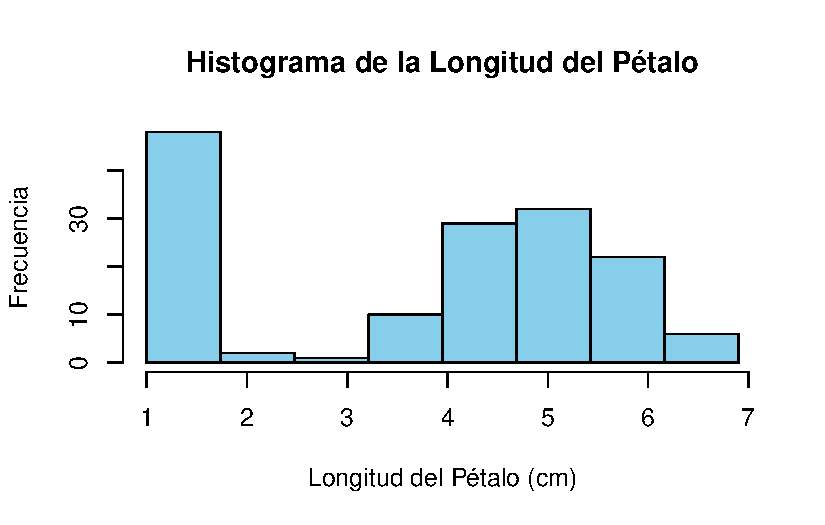
\includegraphics[keepaspectratio]{C5.3_files/figure-pdf/unnamed-chunk-14-1.pdf}}

\textbf{Explicación:}

\begin{enumerate}
\def\labelenumi{\arabic{enumi}.}
\item
  \texttt{hist()}: Función para crear histogramas en R.
\item
  \texttt{longitud\_pedalo}: Variable a graficar.
\item
  \texttt{breaks}: Define los límites de los intervalos de clase. Se
  utiliza \texttt{seq()} para generar una secuencia de valores desde el
  mínimo hasta el máximo de la variable, dividida en \texttt{k\ +\ 1}
  puntos (donde \texttt{k} es el número de clases).
\item
  \texttt{main}, \texttt{xlab}, \texttt{ylab}: Títulos y etiquetas de
  los ejes.
\item
  \texttt{col}, \texttt{border}: Colores de las barras y del borde.
\end{enumerate}

\section{Polígono de Frecuencias}\label{poluxedgono-de-frecuencias}

El polígono de frecuencias es un gráfico de líneas que conecta los
puntos medios de las barras del histograma. Se construye uniendo los
puntos correspondientes a las marcas de clase y sus respectivas
frecuencias.

\textbf{Construcción en R:}

\begin{Shaded}
\begin{Highlighting}[]
\CommentTok{\# Crear el polígono de frecuencias}
\FunctionTok{plot}\NormalTok{(tabla\_freq}\SpecialCharTok{$}\NormalTok{Marca\_Clase,}
\NormalTok{     tabla\_freq}\SpecialCharTok{$}\NormalTok{Frecuencia\_Absoluta, }
     \AttributeTok{type =} \StringTok{"l"}\NormalTok{,  }\CommentTok{\# "l" para líneas}
     \AttributeTok{main =} \StringTok{"Polígono de Frecuencias de la Longitud del Pétalo"}\NormalTok{,}
     \AttributeTok{xlab =} \StringTok{"Longitud del Pétalo (cm)"}\NormalTok{,}
     \AttributeTok{ylab =} \StringTok{"Frecuencia"}\NormalTok{,}
     \AttributeTok{col =} \StringTok{"blue"}\NormalTok{,}
     \AttributeTok{lwd =} \DecValTok{2}\NormalTok{)  }\CommentTok{\# Grosor de la línea}

\CommentTok{\# Agregar puntos en las marcas de clase}
\FunctionTok{points}\NormalTok{(tabla\_freq}\SpecialCharTok{$}\NormalTok{Marca\_Clase,}
\NormalTok{       tabla\_freq}\SpecialCharTok{$}\NormalTok{Frecuencia\_Absoluta, }
       \AttributeTok{col =} \StringTok{"red"}\NormalTok{, }\AttributeTok{pch =} \DecValTok{16}\NormalTok{)  }
\end{Highlighting}
\end{Shaded}

\pandocbounded{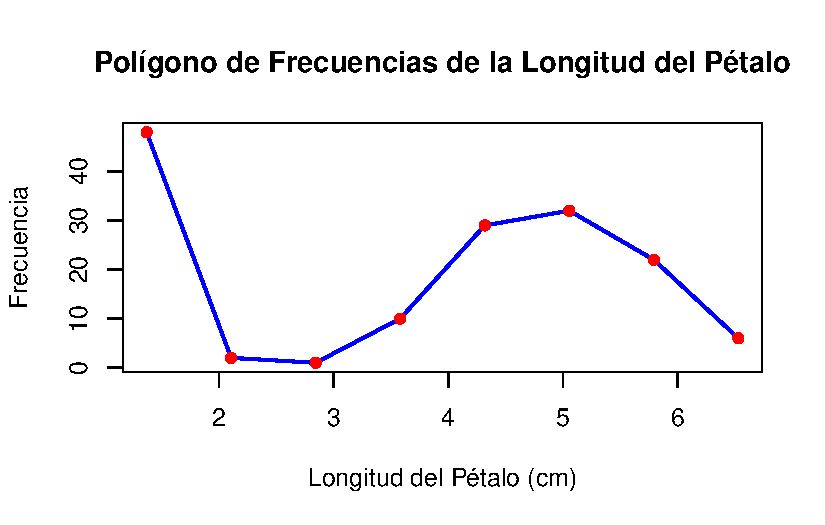
\includegraphics[keepaspectratio]{C5.3_files/figure-pdf/unnamed-chunk-15-1.pdf}}

\begin{Shaded}
\begin{Highlighting}[]
\CommentTok{\# pch = 16 para círculos rellenos}
\end{Highlighting}
\end{Shaded}

\textbf{Explicación:}

\begin{enumerate}
\def\labelenumi{\arabic{enumi}.}
\item
  \texttt{plot(type\ =\ "l")}: Crea un gráfico de líneas.
\item
  \texttt{tabla\_freq\$Marca\_Clase}y
  \texttt{tabla\_freq\$Frecuencia\_Absoluta}: Vectores con las marcas de
  clase y las frecuencias absolutas.
\item
  \texttt{points()}: Agrega puntos en las marcas de clase para resaltar
  los valores.
\end{enumerate}

\section{Ojiva (Polígono de Frecuencias
Acumuladas)}\label{ojiva-poluxedgono-de-frecuencias-acumuladas}

La ojiva es un gráfico de líneas que representa las frecuencias
acumuladas. Se construye uniendo los puntos correspondientes a los
límites superiores de los intervalos de clase y sus respectivas
frecuencias acumuladas.

\textbf{Construcción en R:}

\begin{Shaded}
\begin{Highlighting}[]
\CommentTok{\# Ojiva "Menor Que"}
\FunctionTok{plot}\NormalTok{(tabla\_freq}\SpecialCharTok{$}\NormalTok{Limite\_Superior, tabla\_freq}\SpecialCharTok{$}\NormalTok{Frecuencia\_Acumulada, }
     \AttributeTok{type =} \StringTok{"l"}\NormalTok{,}
     \AttributeTok{main =} \StringTok{"Ojiva \textquotesingle{}Menor Que\textquotesingle{} de la Longitud del Pétalo"}\NormalTok{,}
     \AttributeTok{xlab =} \StringTok{"Longitud del Pétalo (cm)"}\NormalTok{,}
     \AttributeTok{ylab =} \StringTok{"Frecuencia Acumulada"}\NormalTok{,}
     \AttributeTok{col =} \StringTok{"blue"}\NormalTok{)}
\end{Highlighting}
\end{Shaded}

\pandocbounded{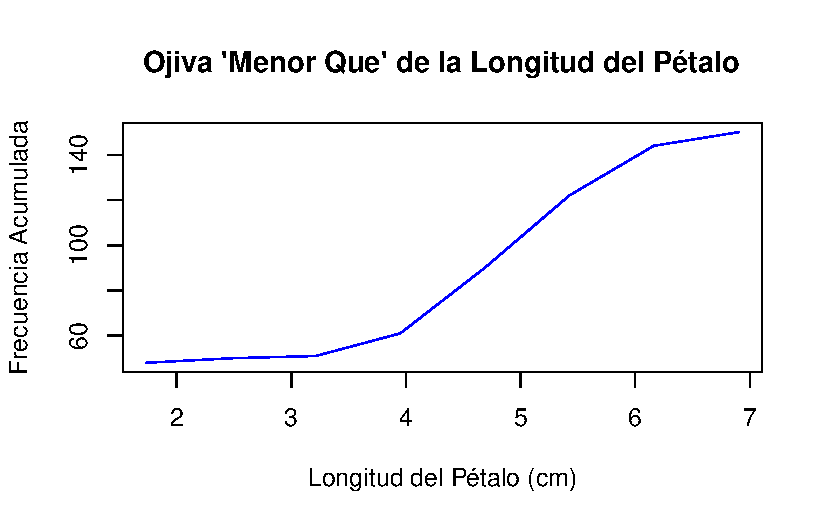
\includegraphics[keepaspectratio]{C5.3_files/figure-pdf/unnamed-chunk-16-1.pdf}}

\begin{Shaded}
\begin{Highlighting}[]
\CommentTok{\# Ojiva "Mayor Que"}
\NormalTok{frecuencia\_acumulada\_mayor\_que }\OtherTok{\textless{}{-}} \FunctionTok{rev}\NormalTok{(}\FunctionTok{cumsum}\NormalTok{(}\FunctionTok{rev}\NormalTok{(tabla\_freq}\SpecialCharTok{$}\NormalTok{Frecuencia\_Absoluta)))}
\FunctionTok{plot}\NormalTok{(tabla\_freq}\SpecialCharTok{$}\NormalTok{Limite\_Inferior, frecuencia\_acumulada\_mayor\_que,}
     \AttributeTok{type =} \StringTok{"l"}\NormalTok{,}
     \AttributeTok{main =} \StringTok{"Ojiva \textquotesingle{}Mayor Que\textquotesingle{} de la Longitud del Pétalo"}\NormalTok{,}
     \AttributeTok{xlab =} \StringTok{"Longitud del Pétalo (cm)"}\NormalTok{,}
     \AttributeTok{ylab =} \StringTok{"Frecuencia Acumulada"}\NormalTok{,}
     \AttributeTok{col =} \StringTok{"red"}\NormalTok{)}
\end{Highlighting}
\end{Shaded}

\pandocbounded{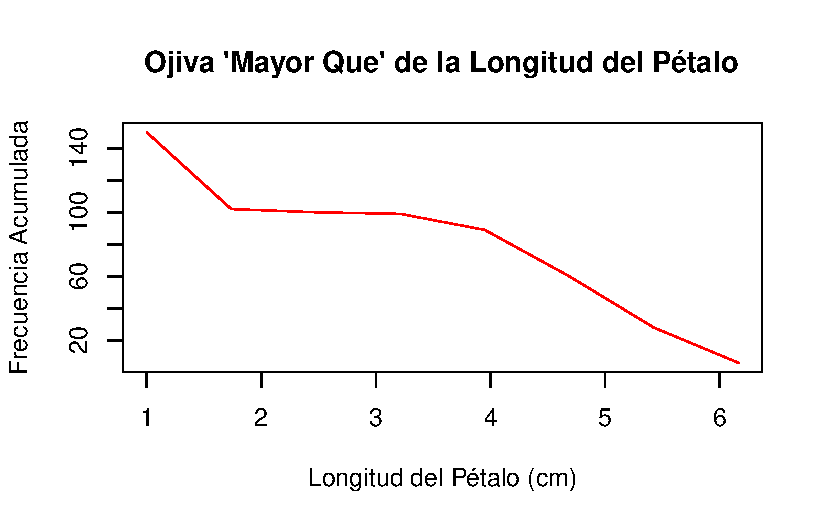
\includegraphics[keepaspectratio]{C5.3_files/figure-pdf/unnamed-chunk-16-2.pdf}}

\section{Gráfico de Barras}\label{gruxe1fico-de-barras}

Aunque el histograma es el gráfico más común para datos agrupados,
también se puede utilizar un gráfico de barras para representar las
frecuencias de cada clase.

\textbf{Construcción en R:}

\begin{Shaded}
\begin{Highlighting}[]
\FunctionTok{barplot}\NormalTok{(tabla\_freq}\SpecialCharTok{$}\NormalTok{Frecuencia\_Absoluta,}
        \AttributeTok{names.arg =}\NormalTok{ tabla\_freq}\SpecialCharTok{$}\NormalTok{Marca\_Clase,}
        \AttributeTok{main =} \StringTok{"Gráfico de Barras de la Longitud del Pétalo"}\NormalTok{,}
        \AttributeTok{xlab =} \StringTok{"Marca de Clase (cm)"}\NormalTok{,}
        \AttributeTok{ylab =} \StringTok{"Frecuencia Absoluta"}\NormalTok{,}
        \AttributeTok{col =} \StringTok{"orange"}\NormalTok{,}
        \AttributeTok{border =} \StringTok{"black"}\NormalTok{)}
\end{Highlighting}
\end{Shaded}

\pandocbounded{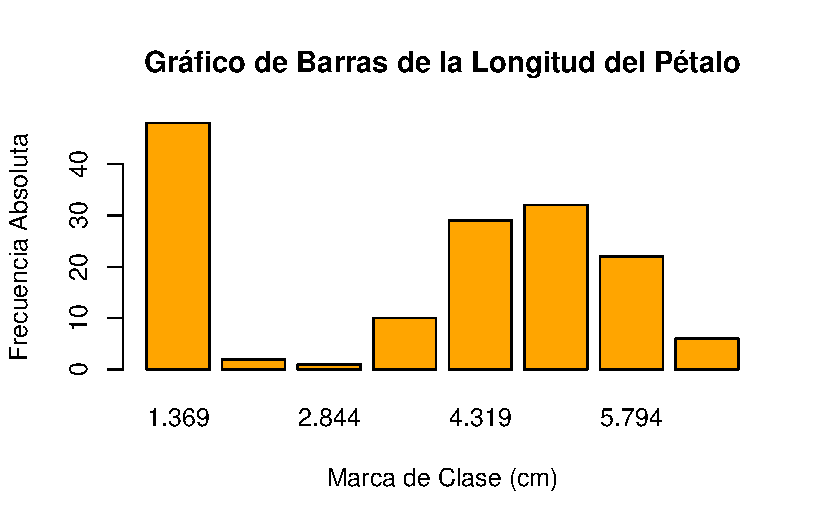
\includegraphics[keepaspectratio]{C5.3_files/figure-pdf/unnamed-chunk-17-1.pdf}}

\textbf{Explicación:}

\begin{enumerate}
\def\labelenumi{\arabic{enumi}.}
\item
  \texttt{barplot()}: Función para crear gráficos de barras en R.
\item
  \texttt{tabla\_freq\$Frecuencia\_Absoluta}: Vector con las frecuencias
  absolutas.
\item
  \texttt{names.arg}: Etiquetas para cada barra (en este caso, las
  marcas de clase).
\end{enumerate}

\section{Cálculos a partir de una tabla de
frecuencias}\label{cuxe1lculos-a-partir-de-una-tabla-de-frecuencias}

No siempre es posible encontrar la base de datos completa para poder
contruir la tabla de frecuencias y realizar las estimaciones, muchas
veces se parte de una tabla de frecuencias debido a la sensibilidad de
los datos, privacidad o porque los datos son muy antiguos y se han
perdido los registos, para este ejemplo se va a explicar como usar las
funciones partiendo de la tabla de frecuencias exportada a un archivo
excel previamente en esta sección:

\subsection{Importar la tabla de
frecuencias}\label{importar-la-tabla-de-frecuencias}

Cabe resaltar que para que esto funcione la tabla de frecuencias que se
vaya a importar debe tener el mismo formato (numero y nombre de columnas
) que la tabla que se muestra a continuación:

\begin{center}
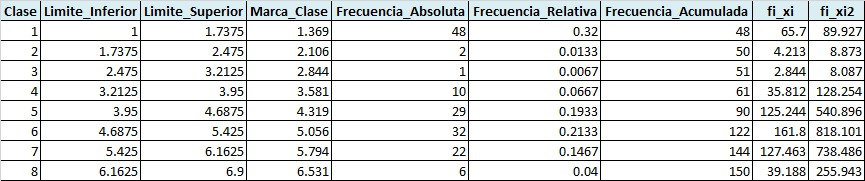
\includegraphics[width=8.33333in,height=\textheight,keepaspectratio]{tabla_frecuencias.jpg}
\end{center}

\begin{Shaded}
\begin{Highlighting}[]
\CommentTok{\#Importar tabla de frecuencias}
\NormalTok{tabla}\OtherTok{\textless{}{-}}\FunctionTok{read\_excel}\NormalTok{(}\StringTok{"tabla\_frecuencias.xlsx"}\NormalTok{)}
\end{Highlighting}
\end{Shaded}

\subsection{Estimación de los parámetros de
agrupación}\label{estimaciuxf3n-de-los-paruxe1metros-de-agrupaciuxf3n}

Una vez importada la tabla de frecuencias adecuadamente se procede a
estimar los parámetros de agrupación a partir de ella, ya que estos son
indispensables para las funciones elaboradas para estimar las medidas de
tendencia central, dispersión y posición relativa.

\begin{Shaded}
\begin{Highlighting}[]
\CommentTok{\# Funcion personalizada para calcular los parametros}
\NormalTok{calcular\_parametros\_desde\_tabla }\OtherTok{\textless{}{-}} \ControlFlowTok{function}\NormalTok{(tabla) \{}
\NormalTok{  n }\OtherTok{\textless{}{-}} \FunctionTok{sum}\NormalTok{(tabla}\SpecialCharTok{$}\NormalTok{Frecuencia\_Absoluta)}
\NormalTok{  x\_min }\OtherTok{\textless{}{-}} \FunctionTok{min}\NormalTok{(tabla}\SpecialCharTok{$}\NormalTok{Limite\_Inferior)}
\NormalTok{  x\_max }\OtherTok{\textless{}{-}} \FunctionTok{max}\NormalTok{(tabla}\SpecialCharTok{$}\NormalTok{Limite\_Superior)}
\NormalTok{  rango }\OtherTok{\textless{}{-}}\NormalTok{ x\_max }\SpecialCharTok{{-}}\NormalTok{ x\_min}
\NormalTok{  k }\OtherTok{\textless{}{-}} \FunctionTok{nrow}\NormalTok{(tabla)}
\NormalTok{  amplitud }\OtherTok{\textless{}{-}}\NormalTok{ (tabla}\SpecialCharTok{$}\NormalTok{Limite\_Superior[}\DecValTok{1}\NormalTok{] }\SpecialCharTok{{-}}\NormalTok{ tabla}\SpecialCharTok{$}\NormalTok{Limite\_Inferior[}\DecValTok{1}\NormalTok{])}

  \FunctionTok{return}\NormalTok{(}\FunctionTok{list}\NormalTok{(}
    \AttributeTok{n =}\NormalTok{ n,}
    \AttributeTok{x\_min =}\NormalTok{ x\_min,}
    \AttributeTok{x\_max =}\NormalTok{ x\_max,}
    \AttributeTok{rango =}\NormalTok{ rango,}
    \AttributeTok{k =}\NormalTok{ k,}
    \AttributeTok{amplitud =}\NormalTok{ amplitud}
\NormalTok{  ))}
\NormalTok{\}}
\end{Highlighting}
\end{Shaded}

Una vez cargada la funcion al entorno de trabajo esta se utiliza con la
tabla de frecuencias previamente importada para estimar los parametros
de agrupacion

\begin{Shaded}
\begin{Highlighting}[]
\CommentTok{\# Estimar los parametros de agrupacion a partir de la tabla de frecuencias}
\NormalTok{parametros\_tabla }\OtherTok{\textless{}{-}} \FunctionTok{calcular\_parametros\_desde\_tabla}\NormalTok{(tabla)}
\end{Highlighting}
\end{Shaded}

\subsection{Estimación de los parámetros con las mismas
funciones}\label{estimaciuxf3n-de-los-paruxe1metros-con-las-mismas-funciones}

Una vez ya se ha importado la tabla de frecuencias y estimado los
parametros de agrupacion a partir de la tabla de frecuencias es posible
usar las funciones previamente establecidas para calculas los parametros
como se muestra a continuación:

\begin{enumerate}
\def\labelenumi{\arabic{enumi}.}
\item
  \textbf{Medidas de tendencia central}

\begin{Shaded}
\begin{Highlighting}[]
\CommentTok{\# Calcular medidas}
\NormalTok{tendencia\_tabla }\OtherTok{\textless{}{-}} \FunctionTok{calcular\_tendencia\_central}\NormalTok{(tabla, parametros\_tabla)}

\CommentTok{\# Mostrar resultados }
\NormalTok{tendencia\_tabla}
\end{Highlighting}
\end{Shaded}

\begin{verbatim}
$media
[1] 3.748427

$mediana
[1] 4.306034

$moda
[1] 1.376596
\end{verbatim}
\item
  \textbf{Medidas de dispersión}

\begin{Shaded}
\begin{Highlighting}[]
\CommentTok{\# Calcular medidas de dispersión}
\NormalTok{dispersion\_tabla }\OtherTok{\textless{}{-}} \FunctionTok{calcular\_dispersion}\NormalTok{(tabla, }
\NormalTok{                                        parametros\_tabla, }
\NormalTok{                                        tendencia\_tabla}\SpecialCharTok{$}\NormalTok{media)}

\CommentTok{\# Mostrar los resultados}
\NormalTok{dispersion\_tabla}
\end{Highlighting}
\end{Shaded}

\begin{verbatim}
$rango
[1] 5.9

$varianza
[1] 3.22793

$desviacion_std
[1] 1.796644

$cv
[1] 47.93062
\end{verbatim}
\item
  \textbf{Medidas de posición relativa}

\begin{Shaded}
\begin{Highlighting}[]
\CommentTok{\# Calcular Q1 y P80}
\NormalTok{Q1\_tabla }\OtherTok{\textless{}{-}} \FunctionTok{calcular\_posicion\_relativa}\NormalTok{(tabla, parametros\_tabla,}
                                       \DecValTok{1}\NormalTok{, }\StringTok{"cuartil"}\NormalTok{);Q1\_tabla}
\end{Highlighting}
\end{Shaded}

\begin{verbatim}
[1] 1.576172
\end{verbatim}

\begin{Shaded}
\begin{Highlighting}[]
\NormalTok{P80\_tabla }\OtherTok{\textless{}{-}} \FunctionTok{calcular\_posicion\_relativa}\NormalTok{(tabla, parametros\_tabla,}
                                        \DecValTok{80}\NormalTok{, }\StringTok{"percentil"}\NormalTok{);P80\_tabla}
\end{Highlighting}
\end{Shaded}

\begin{verbatim}
[1] 5.378906
\end{verbatim}
\end{enumerate}

Como se puede observar siempre y cuando la tabla de frecuencias siga el
formato propuesto las funciones seguirán operando con normalidad
partiendo desde una base de datos completa o únicamente desde una tabla
de frecuencias, cabe resaltar que el ajustar el formato de la tabla de
frecuencias cuando se trabaja con una tabla de frecuencias y no con una
base de datos completa es una tarea adicional que se debe llevar a cabo
previo al análisis.

\part{6. Introducción a probabilidades}

\bookmarksetup{startatroot}

\chapter{Introducción a
probabilidades}\label{introducciuxf3n-a-probabilidades-1}

La mayor parte de los problemas en estadística involucran elementos de
incertidumbre, ya que usualmente no es posible determinar
anticipadamente las características de una población desconocida o
prever las consecuencias exactas de la toma de una decisión. Por lo
tanto, es conveniente disponer de una medida que exprese esa
incertidumbre en términos de una escala numérica. Esta medida es la
\textbf{probabilidad} (López \& González, 2018).

En el contexto agronómico, la probabilidad permite modelar y cuantificar
la variabilidad inherente en los procesos biológicos, climáticos y
productivos. Por ejemplo, se puede utilizar para evaluar la probabilidad
de ocurrencia de plagas, el éxito de tratamientos fitosanitarios, o la
variabilidad en rendimientos de cultivos.

\section{Conceptos Fundamentales}\label{conceptos-fundamentales}

\subsection{Experimento y Experimento
Aleatorio}\label{experimento-y-experimento-aleatorio}

Un \textbf{experimento} es el proceso mediante el cual se obtiene una
observación o medida de un fenómeno. Cuando el resultado del experimento
no puede preverse con certeza debido a la variabilidad inherente del
fenómeno, se denomina \textbf{experimento aleatorio} (López \& González,
2018).

\textbf{Ejemplos de experimentos aleatorios:}

\begin{enumerate}
\def\labelenumi{\arabic{enumi}.}
\item
  Lanzamiento de un dado y observación del número mostrado en la cara
  superior
\item
  Lanzamiento de una moneda cuatro veces y observación del número de
  caras obtenido
\item
  Prueba de duración de una lámpara, anotando el tiempo transcurrido
  desde que se enciende hasta que se quema
\item
  Cruzamiento de animales y observación del sexo del primero que nace
\item
  Conteo del número de larvas de gusano cogollero en plantas de maíz
\item
  Conteo del número de piezas defectuosas producidas en una línea de
  producción durante 24 horas
\end{enumerate}

\subsection{Espacio Muestral}\label{espacio-muestral}

El \textbf{espacio muestral} es el conjunto de todos los posibles
resultados de un experimento aleatorio. Se denota con el símbolo
\(\Omega\) (López \& González, 2018).

\textbf{Ejemplos de espacios muestrales:}

\begin{enumerate}
\def\labelenumi{\arabic{enumi}.}
\item
  Para el lanzamiento de un dado: \(\Omega = \{1, 2, 3, 4, 5, 6\}\)
\item
  Para el lanzamiento de una moneda cuatro veces:
  \(\Omega = \{0, 1, 2, 3, 4\}\)
\item
  Para la duración de una lámpara: \(\Omega = \{t | t \geq 0\}\)
\item
  Para el sexo de una cría: \(\Omega = \{\text{Macho, Hembra}\}\)
\item
  Para el conteo de larvas: \(\Omega = \{0, 1, 2, ...\}\)
\end{enumerate}

\subsection{Evento}\label{evento}

Un \textbf{evento} A es un subconjunto del espacio muestral \(\Omega\).
En terminología de conjuntos, un evento es simplemente un conjunto de
resultados posibles del experimento aleatorio. Los eventos se denotan
con letras mayúsculas como A, B, C, etc. (López \& González, 2018).

\textbf{Ejemplos de eventos:}

\begin{enumerate}
\def\labelenumi{\arabic{enumi}.}
\item
  \(A_1\)\hspace{0pt}: Sale un número par en el lanzamiento de un dado,
  \(A_1 = \{2, 4, 6\}\)
\item
  \(A_2\)\hspace{0pt}: Ocurren dos caras en cuatro lanzamientos,
  \(A_2 = \{2\}\)
\item
  \(A_3\)\hspace{0pt}: La lámpara se quema en menos de 3 horas,
  \(A_3 = \{t | 0 \leq t < 3\}\)
\end{enumerate}

\section{Métodos para Asignar
Probabilidades}\label{muxe9todos-para-asignar-probabilidades}

Independientemente del método utilizado, se deben satisfacer dos
requisitos básicos:

\begin{enumerate}
\def\labelenumi{\arabic{enumi}.}
\item
  Los valores de probabilidad asignados a cada resultado experimental
  deben estar entre 0 y 1:
  \[\LARGE 0 \leq P(E_i) \leq 1, \text{ para toda } i\]
\item
  La suma de todas las probabilidades de resultados experimentales debe
  ser 1: \[\LARGE \sum_{i=1}^{k} P(E_i) = 1\]
\end{enumerate}

\subsection{Método Clásico}\label{muxe9todo-cluxe1sico}

Si un evento A puede ocurrir en \(h\) maneras diferentes de un número
total de \(n\) maneras posibles, todas igualmente probables, entonces la
probabilidad del evento es:

\[\LARGE P(A) = \frac{h}{n} = \frac{\text{número de resultados favorables}}{\text{número de resultados posibles}}\]

\textbf{Ejemplo:} En el lanzamiento de dos dados honestos, calcule las
probabilidades de los siguientes eventos:

\textbf{A:} La suma de los valores es igual a 7

\textbf{B:} Los resultados en los dados son iguales

\textbf{C:} La suma de los valores es 9 o más

El espacio muestral contiene 36 resultados posibles. Contando los casos
favorables:

\begin{itemize}
\item
  Para A: \({(1,6),(2,5),(3,4),(4,3),(5,2),(6,1)}\), entonces
  \(P(A) = \frac{6}{36} = 0.167\)
\item
  Para B: \({(1,1), (2,2), (3,3), (4,4), (5,5), (6,6)}\), entonces
  \(P(B) = \frac{6}{36} = 0.167\)
\item
  Para C: 10 casos favorables, entonces
  \(P(C) = \frac{10}{36} = 0.278P\)
\end{itemize}

\subsection{Método de la Frecuencia
Relativa}\label{muxe9todo-de-la-frecuencia-relativa}

Si después de nnn repeticiones de un experimento donde nnn es ``muy
grande'', un evento ocurre hhh veces, entonces la probabilidad del
evento es:

\[\huge P(A) = \frac{h}{n}\]

\textbf{Ejemplo:} Si se lanza una moneda 1000 veces y resultan 532
caras, se puede estimar que:
\[\Large P(\text{cara}) = \frac{532}{1000} = 0.532\]

\subsection{Método Subjetivo}\label{muxe9todo-subjetivo}

Este método está basado en el juicio personal. Se puede usar cualquier
dato disponible junto con la experiencia e intuición del investigador.

\section{Relaciones Básicas de
Probabilidad}\label{relaciones-buxe1sicas-de-probabilidad}

\subsection{Complemento de un Evento}\label{complemento-de-un-evento}

Dado un evento A, el \textbf{complemento} de A se define como el evento
formado por todos los puntos muestrales que no están en A, y se
representa por \(A^c\).

\[\LARGE P(A) + P(A^c) = 1\]

Por lo tanto: \(P(A) = 1 - P(A^c)\)

\subsection{Ley Aditiva}\label{ley-aditiva}

La ley aditiva es útil cuando se tienen dos eventos y se desea conocer
la probabilidad de que ocurra por lo menos uno de ellos. Para eventos A
y B:

\[\Large P(A \cup B) = P(A) + P(B) - P(A \cap B)\]

\textbf{Ejemplo:} El gerente de personal de una empresa agroforestal
encontró que el 30\% de los empleados que salieron lo hicieron por
insatisfacción salarial, el 20\% por insatisfacción laboral, y el 12\%
por ambas razones.

Sean:

\begin{enumerate}
\def\labelenumi{\arabic{enumi}.}
\item
  S: evento de salida por salario
\item
  W: evento de salida por trabajo
\end{enumerate}

\[\large P(S \cup W) = P(S) + P(W) - P(S \cap W) = 0.30 + 0.20 - 0.12 = 0.38\]

\subsection{Eventos Mutuamente
Excluyentes}\label{eventos-mutuamente-excluyentes}

Dos eventos son \textbf{mutuamente excluyentes} si no tienen puntos
muestrales en común, es decir, \(P(A \cap B) = 0\).

Para eventos mutuamente excluyentes:\\
\[\LARGE P(A \cup B) = P(A) + P(B)\]

\section{Probabilidad Condicional}\label{probabilidad-condicional}

La \textbf{probabilidad condicional} de un evento A dado que ha ocurrido
B se denota como \(P(A|B)\) y se define como:

\[\LARGE P(A|B) = \frac{P(A \cap B)}{P(B)}, \text{ siempre que } P(B) > 0\]

Esta notación se lee como ``la probabilidad de A dado B'' y representa
la probabilidad de que ocurra A sabiendo que B ya ha ocurrido.

\textbf{Ejemplo:} En una facultad de agronomía se tiene la siguiente
distribución de estudiantes:

\begin{longtable}[]{@{}llll@{}}
\toprule\noalign{}
Carrera & Masculino & Femenino & Total \\
\midrule\noalign{}
\endhead
\bottomrule\noalign{}
\endlastfoot
Agronomía & 160 & 40 & 200 \\
Forestal & 30 & 10 & 40 \\
Agroindustrial & 15 & 10 & 25 \\
\textbf{Total} & \textbf{205} & \textbf{60} & \textbf{265} \\
\end{longtable}

Dado que un alumno cursa Agronomía (A), ¿cuál es la probabilidad de que
sea masculino (H)?

\[\Large P(H|A) = \frac{P(H \cap A)}{P(A)} = \frac{160/265}{200/265} = \frac{160}{200} = 0.80\]

\section{Eventos Independientes}\label{eventos-independientes}

Dos eventos A y B son \textbf{independientes} si:

\[\Large P(A|B) = P(A) \text{ o } P(B|A) = P(B)\]

De lo contrario, los eventos son dependientes.

\section{Ley Multiplicativa}\label{ley-multiplicativa}

Mientras que la ley aditiva se utiliza para determinar la probabilidad
de una unión entre dos eventos, la \textbf{ley multiplicativa} se usa
para determinar la probabilidad de una intersección de dos eventos:

\[\LARGE P(A \cap B) = P(B) \cdot P(A|B)\]

o también:

\[\LARGE P(A \cap B) = P(A) \cdot P(B|A)\]

\subsection{Ley Multiplicativa para Eventos
Independientes}\label{ley-multiplicativa-para-eventos-independientes}

Para eventos independientes:

\[\LARGE P(A \cap B) = P(A) \cdot P(B)\]

\textbf{Ejemplo:} El gerente de una gasolinera sabe que el 80\% de los
clientes usan tarjeta de crédito. ¿Cuál es la probabilidad de que dos
clientes consecutivos usen tarjeta de crédito?

\[\LARGE P(A \cap B) = P(A) \cdot P(B) = 0.8 \times 0.8 = 0.64\]

\section{Diagramas de Árbol}\label{diagramas-de-uxe1rbol}

Un \textbf{diagrama de árbol} es una herramienta gráfica que se emplea
frecuentemente en conexión con el principio multiplicativo. Debido a su
apariencia, permite visualizar todos los posibles resultados de un
experimento compuesto y facilita el cálculo de probabilidades.

\textbf{Ejemplo:} Si un hombre tiene 2 camisas (\(S_1, S_2\)) y 4
corbatas (\(T_1, T_2, T_3, T_4\)), entonces tiene \(2 \times 4 = 8\)
maneras de escoger una camisa y luego una corbata.

El diagrama de árbol correspondiente sería:

\begin{center}
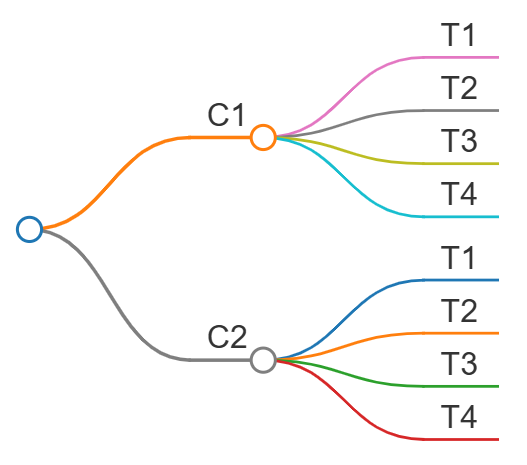
\includegraphics[width=4.6875in,height=\textheight,keepaspectratio]{diagrama_ct.png}
\end{center}

\subsection{Uso de Diagramas de Árbol en Probabilidad
Condicional}\label{uso-de-diagramas-de-uxe1rbol-en-probabilidad-condicional}

Los diagramas de árbol son especialmente útiles para problemas de
probabilidad condicional, donde las probabilidades en las ramas
posteriores dependen de los resultados de las ramas anteriores.

\textbf{Ejemplo aplicado:} Una empresa agrícola tiene tres proveedores
de semillas. El proveedor A suministra el 40\% de las semillas, el
proveedor B el 35\%, y el proveedor C el 25\%. Las tasas de germinación
son del 95\%, 90\%, y 85\% respectivamente.

El diagrama de árbol sería:

\begin{center}
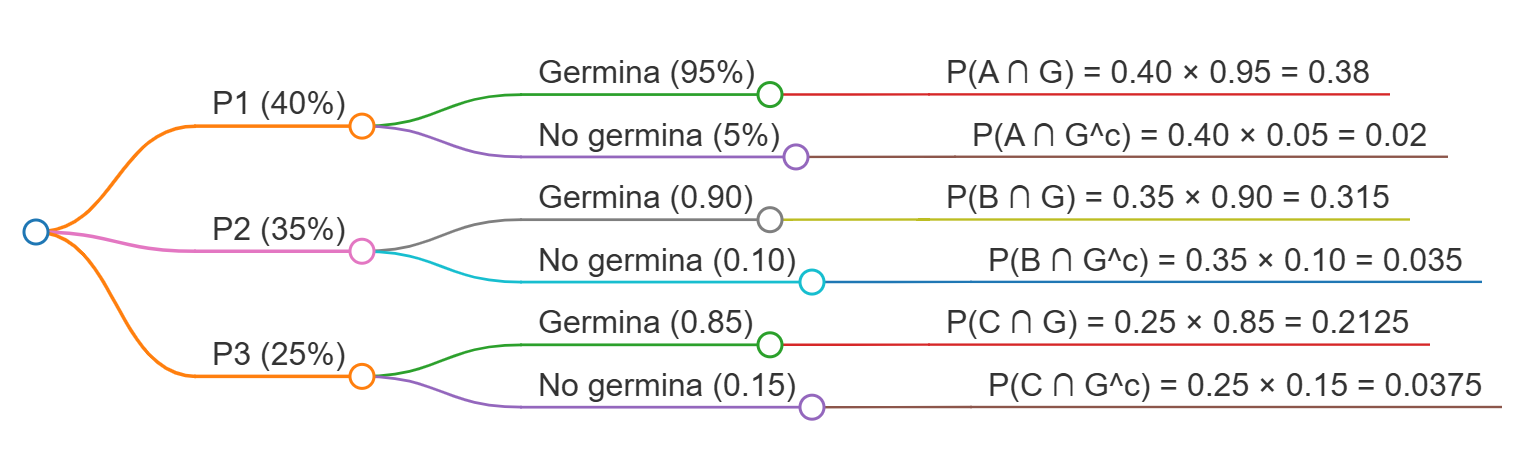
\includegraphics[width=6.77083in,height=\textheight,keepaspectratio]{arbol_semillas.png}
\end{center}

\section{Teorema de Bayes}\label{teorema-de-bayes}

El \textbf{teorema de Bayes} también se conoce como ``probabilidad de
las causas'', es decir, la probabilidad de un hecho anterior sabiendo la
probabilidad de un hecho posterior. Se basa en que los eventos definidos
sobre un espacio muestral son particiones del mismo.

Si \(A_1, A_2, A_3, ..., A_n\)\hspace{0pt} son eventos mutuamente
excluyentes y exhaustivos, y \(B\) es un evento observado, entonces:

\[\LARGE P(A_i|B) = \frac{P(A_i) \cdot P(B|A_i)}{\sum_{j=1}^{n} P(A_j) \cdot P(B|A_j)}\]

donde:

\begin{enumerate}
\def\labelenumi{\arabic{enumi}.}
\item
  \(P(A_i)\) son las probabilidades a priori
\item
  \(P(B|A_i)\) son las probabilidades condicionales
\item
  \(P(A_i|B)\) son las probabilidades a posteriori
\end{enumerate}

\textbf{Ejemplo resuelto:} Una fábrica con 3 sucursales produce 40\%,
35\% y 25\% del total de la producción. Tienen porcentajes de artículos
defectuosos de 4\%, 6\% y 8\%, respectivamente. Si se elige
aleatoriamente un artículo:

a) ¿Cuál es la probabilidad de que no sea defectuoso?

Usando la ley de probabilidad total:\\
\[\large P(C) = P(A_1) \cdot P(C|A_1) + P(A_2) \cdot P(C|A_2) + P(A_3) \cdot P(C|A_3)\]

\[\large P(C) = 0.40 \times 0.96 + 0.35 \times 0.94 + 0.25 \times 0.92 = 0.943\]

b) Si resultó defectuoso, ¿cuál es la probabilidad de que proceda de la
primera sucursal?

Primero calculamos \[\Large P(B) = 1 - P(C) = 1 - 0.943 = 0.057\]

Luego aplicamos Bayes:\\
\[\Large P(A_1|B) = \frac{P(A_1) \cdot P(B|A_1)}{P(B)} = \frac{0.40 \times 0.04}{0.057} = 0.2807\]

\subsection{Tabla de Análisis para el Teorema de
Bayes}\label{tabla-de-anuxe1lisis-para-el-teorema-de-bayes}

\begin{longtable}[]{@{}
  >{\raggedright\arraybackslash}p{(\linewidth - 8\tabcolsep) * \real{0.2000}}
  >{\raggedright\arraybackslash}p{(\linewidth - 8\tabcolsep) * \real{0.2000}}
  >{\raggedright\arraybackslash}p{(\linewidth - 8\tabcolsep) * \real{0.2000}}
  >{\raggedright\arraybackslash}p{(\linewidth - 8\tabcolsep) * \real{0.2000}}
  >{\raggedright\arraybackslash}p{(\linewidth - 8\tabcolsep) * \real{0.2000}}@{}}
\toprule\noalign{}
\begin{minipage}[b]{\linewidth}\raggedright
Eventos
\end{minipage} & \begin{minipage}[b]{\linewidth}\raggedright
Probabilidades previas
\end{minipage} & \begin{minipage}[b]{\linewidth}\raggedright
Probabilidades condicionales
\end{minipage} & \begin{minipage}[b]{\linewidth}\raggedright
Probabilidades conjuntas
\end{minipage} & \begin{minipage}[b]{\linewidth}\raggedright
Probabilidades posteriores
\end{minipage} \\
\midrule\noalign{}
\endhead
\bottomrule\noalign{}
\endlastfoot
\(A_i\)\hspace{0pt} & \(P(A_i)\) & \(P(C)\) & \(P(A_i) \cdot P(C|A_i)\)
& \(P(A_i|  B)\) \\
\(A_1\)\hspace{0pt} & 0.40 & 0.04 & 0.016 & 0.2807 \\
\(A_2\)\hspace{0pt} & 0.35 & 0.06 & 0.021 & 0.3684 \\
\(A_3\)\hspace{0pt} & 0.25 & 0.08 & 0.020 & 0.3509 \\
\textbf{Total} & \textbf{1.00} & & \textbf{P(B) = 0.057} &
\textbf{1.0000} \\
\end{longtable}

\section{Notación Correcta para
Probabilidades}\label{notaciuxf3n-correcta-para-probabilidades}

Es fundamental utilizar la notación correcta para evitar confusiones:

\begin{enumerate}
\def\labelenumi{\arabic{enumi}.}
\item
  \(P(A)\): Probabilidad marginal del evento A
\item
  \(P(A \cap B)\): Probabilidad conjunta de A y B (intersección)
\item
  \(P(A \cup B)\): Probabilidad de la unión de A y B
\item
  \(P(A|B)\): Probabilidad condicional de A dado B
\item
  \(P(A^c)\): Probabilidad del complemento de A
\item
  \(A \perp B\): A y B son independientes
\end{enumerate}

\part{7. Distribuciones de probabilidad discretas}

\bookmarksetup{startatroot}

\chapter{Distribuciones Binomial y Poisson en
R}\label{distribuciones-binomial-y-poisson-en-r}

\section{Introducción}\label{introducciuxf3n-1}

El estudio de las distribuciones de probabilidad constituye uno de los
pilares fundamentales de la estadística aplicada. En el contexto de las
ciencias agronómicas, estas herramientas matemáticas permiten modelar y
analizar fenómenos aleatorios que ocurren frecuentemente en la
investigación y práctica agrícola. Las distribuciones binomial y de
Poisson, como distribuciones discretas, son especialmente útiles para
describir eventos de conteo, tales como el número de semillas
germinadas, la cantidad de plagas observadas en una parcela, o la
ocurrencia de eventos climáticos adversos.

Según López y González (2018), las variables aleatorias discretas son
aquellas que pueden tomar un conjunto finito o numerable de valores,
generalmente asociados a conteos de eventos. El software estadístico R
proporciona funciones específicas para el cálculo de probabilidades en
estas distribuciones, facilitando el análisis estadístico y la toma de
decisiones basada en evidencia.

\section{Distribución Binomial}\label{distribuciuxf3n-binomial}

\subsection{Características y
definición}\label{caracteruxedsticas-y-definiciuxf3n}

La distribución binomial describe el número de éxitos obtenidos en una
secuencia de ensayos independientes, donde cada ensayo presenta
únicamente dos posibles resultados: éxito o fracaso. López y González
(2018) establecen que un experimento binomial posee las siguientes
características fundamentales:

\begin{enumerate}
\def\labelenumi{\arabic{enumi}.}
\item
  Consta de \(n\) ensayos o pruebas idénticas (ensayos de Bernoulli)
\item
  Cada prueba puede tener uno de dos resultados posibles (éxito o
  fracaso)
\item
  La probabilidad de un éxito en una sola prueba es igual a \(p\), y
  permanece constante de una prueba a otra. La probabilidad de fracaso
  es igual a \((1-p)\) y se denota con la letra \(q\)
\item
  El resultado obtenido en cada prueba es independiente de los
  resultados obtenidos anteriormente
\end{enumerate}

La distribución binomial se representa como \(B(n,p)\), siendo \(n\) y
\(p\) los parámetros de dicha distribución.

\subsection{Función de probabilidad}\label{funciuxf3n-de-probabilidad}

La función de probabilidad de la distribución binomial se expresa
matemáticamente como:

\[\LARGE P(X = x) = \binom{n}{x} p^x q^{n-x}, \quad x = 0,1,2,\ldots,n\]

donde:

\begin{enumerate}
\def\labelenumi{\arabic{enumi}.}
\item
  \(X\) es la variable aleatoria que representa el número de éxitos
\item
  \(x\) es el número de éxitos observados
\item
  \(n\) es el número total de ensayos
\item
  \(p\) es la probabilidad de éxito en cada ensayo
\item
  \(q = 1-p\) es la probabilidad de fracaso
\item
  \(\binom{n}{x} = \frac{n!}{x!(n-x)!}\) es el coeficiente binomial
\end{enumerate}

\subsection{Parámetros de la distribución
binomial}\label{paruxe1metros-de-la-distribuciuxf3n-binomial}

Los parámetros de tendencia central y dispersión de la distribución
binomial son:

\begin{enumerate}
\def\labelenumi{\arabic{enumi}.}
\item
  Media: \(E(X) = np\)
\item
  Varianza: \(V(X) = npq\)
\end{enumerate}

\section{Cálculo de probabilidades binomiales en
R}\label{cuxe1lculo-de-probabilidades-binomiales-en-r}

El software R proporciona funciones específicas para el cálculo de
probabilidades binomiales. A continuación se describen las funciones
principales y sus argumentos.

\subsection{Función para calcular P(X =
x)}\label{funciuxf3n-para-calcular-px-x}

Para calcular la probabilidad de obtener exactamente xxx éxitos, se
utiliza la función:

\[\LARGE \texttt{dbinom(x, size, prob)} \]

\textbf{Argumentos en orden:}

\begin{enumerate}
\def\labelenumi{\arabic{enumi}.}
\item
  \(\texttt{x}\): número de éxitos deseados (valor específico de la
  variable aleatoria)
\item
  \(\texttt{size}\): número total de ensayos (\(n\))
\item
  \(\texttt{prob}\): probabilidad de éxito en cada ensayo (\(p\))
\end{enumerate}

\subsection{Función para calcular P(X ≤ x) y P(X \textgreater{}
x)}\label{funciuxf3n-para-calcular-px-x-y-px-x}

Para calcular probabilidades acumuladas, se utiliza la función:

\[\LARGE \texttt{pbinom(q, size, prob, lower.tail)}\]

\textbf{Argumentos en orden:}

\begin{enumerate}
\def\labelenumi{\arabic{enumi}.}
\item
  \(\texttt{q}\): valor hasta el cual se desea calcular la probabilidad
  acumulada
\item
  \(\texttt{size}\): número total de ensayos (nnn)
\item
  \(\texttt{prob}\): probabilidad de éxito en cada ensayo (ppp)
\item
  \(\texttt{lower.tail}\): argumento lógico que indica si se calcula
  \(P(X \leq x) (\texttt{TRUE}, por defecto)\) o
  \(P(X > x) (\texttt{FALSE})\)
\end{enumerate}

\subsection{Ejemplo práctico: Germinación de
semillas}\label{ejemplo-pruxe1ctico-germinaciuxf3n-de-semillas}

Supóngase que se siembran 20 semillas de maíz y se sabe que la
probabilidad de germinación de cada semilla es de 0.8. Se desea calcular
las siguientes probabilidades:

\subsubsection{Caso 1: P(X = 16) - Probabilidad de que germinen
exactamente 16
semillas}\label{caso-1-px-16---probabilidad-de-que-germinen-exactamente-16-semillas}

\begin{Shaded}
\begin{Highlighting}[]
\FunctionTok{dbinom}\NormalTok{(}\DecValTok{16}\NormalTok{, }\DecValTok{20}\NormalTok{, }\FloatTok{0.8}\NormalTok{)}
\end{Highlighting}
\end{Shaded}

\begin{verbatim}
[1] 0.2181994
\end{verbatim}

\subsubsection{Caso 2: P(X ≤ 15) - Probabilidad de que germinen 15 o
menos
semillas}\label{caso-2-px-15---probabilidad-de-que-germinen-15-o-menos-semillas}

\begin{Shaded}
\begin{Highlighting}[]
\FunctionTok{pbinom}\NormalTok{(}\DecValTok{15}\NormalTok{, }\DecValTok{20}\NormalTok{, }\FloatTok{0.8}\NormalTok{)}
\end{Highlighting}
\end{Shaded}

\begin{verbatim}
[1] 0.3703517
\end{verbatim}

\subsubsection{Caso 3: P(X \textgreater{} 18) - Probabilidad de que
germinen más de 18
semillas}\label{caso-3-px-18---probabilidad-de-que-germinen-muxe1s-de-18-semillas}

\begin{Shaded}
\begin{Highlighting}[]
\FunctionTok{pbinom}\NormalTok{(}\DecValTok{18}\NormalTok{, }\DecValTok{20}\NormalTok{, }\FloatTok{0.8}\NormalTok{, }\AttributeTok{lower.tail =} \ConstantTok{FALSE}\NormalTok{)}
\end{Highlighting}
\end{Shaded}

\begin{verbatim}
[1] 0.06917529
\end{verbatim}

\section{Distribución de Poisson}\label{distribuciuxf3n-de-poisson}

\subsection{Características y
definición}\label{caracteruxedsticas-y-definiciuxf3n-1}

La distribución de Poisson, desarrollada por Simeón Dennis Poisson
(1781-1840), es un modelo apropiado para describir el número de eventos
raros que ocurren en un intervalo de tiempo o espacio específico. López
y González (2018) indican que esta distribución es útil para modelar
eventos con las siguientes características:

\begin{enumerate}
\def\labelenumi{\arabic{enumi}.}
\item
  Los eventos ocurren de manera independiente
\item
  La tasa promedio de ocurrencia permanece constante
\item
  Los eventos son raros o poco frecuentes
\end{enumerate}

\subsection{Función de probabilidad}\label{funciuxf3n-de-probabilidad-1}

Una variable aleatoria \(X\) tiene distribución de Poisson con parámetro
\(\lambda > 0\), si su función de probabilidad está dada por:

\[\Large P(X = x) = \frac{e^{-\lambda} \lambda^x}{x!}, \quad x = 0,1,2,\ldots  \]

donde:

\begin{enumerate}
\def\labelenumi{\arabic{enumi}.}
\item
  \(\lambda\) representa el número medio de ocurrencias por intervalo de
  tiempo
\item
  \(e = 2.71828\) es la base de los logaritmos naturales
\end{enumerate}

La notación utilizada es: \(X \sim Po(\lambda)\)

\subsection{Parámetros de la distribución de
Poisson}\label{paruxe1metros-de-la-distribuciuxf3n-de-poisson}

Los parámetros de la distribución de Poisson son:

\begin{enumerate}
\def\labelenumi{\arabic{enumi}.}
\item
  Media:\(E(X) = \lambda\)
\item
  Varianza: \(V(X) = \lambda\)
\end{enumerate}

\section{Cálculo de probabilidades de Poisson en
R}\label{cuxe1lculo-de-probabilidades-de-poisson-en-r}

\subsection{Función para calcular P(X =
x)}\label{funciuxf3n-para-calcular-px-x-1}

Para calcular la probabilidad de observar exactamente \(x\) eventos, se
utiliza:

\[\LARGE \texttt{dpois(x, lambda)}\]

\textbf{Argumentos en orden:}

\begin{enumerate}
\def\labelenumi{\arabic{enumi}.}
\item
  \(\texttt{x}\): número de eventos observados
\item
  \(\texttt{lambda}\): tasa promedio de ocurrencia (\(\lambda\))
\end{enumerate}

\subsection{Función para calcular P(X ≤ x) y P(X \textgreater{}
x)}\label{funciuxf3n-para-calcular-px-x-y-px-x-1}

Para probabilidades acumuladas, se utiliza:

\[\LARGE \texttt{ppois(q, lambda, lower.tail)}  \]

\textbf{Argumentos en orden:}

\begin{enumerate}
\def\labelenumi{\arabic{enumi}.}
\item
  \(\texttt{q}\): valor hasta el cual se desea calcular la probabilidad
  acumulada
\item
  \(\texttt{lambda}\): tasa promedio de ocurrencia (λ\lambdaλ)
\item
  \(\texttt{lower.tail}\): argumento lógico para \(P(X \leq x)\)
  (\(\texttt{TRUE}\)) o \(P(X > x)\) (\(\texttt{FALSE}\))
\end{enumerate}

\subsection{Ejemplo práctico: Incidencia de
plagas}\label{ejemplo-pruxe1ctico-incidencia-de-plagas}

Supóngase que en un cultivo de tomate se observa un promedio de 3 plagas
por metro cuadrado. Se desea calcular las siguientes probabilidades:

\subsubsection{Caso 1: P(X = 5) - Probabilidad de observar exactamente 5
plagas}\label{caso-1-px-5---probabilidad-de-observar-exactamente-5-plagas}

\begin{Shaded}
\begin{Highlighting}[]
\FunctionTok{dpois}\NormalTok{(}\DecValTok{5}\NormalTok{, }\DecValTok{3}\NormalTok{)}
\end{Highlighting}
\end{Shaded}

\begin{verbatim}
[1] 0.1008188
\end{verbatim}

\subsubsection{Caso 2: P(X ≤ 2) - Probabilidad de observar 2 o menos
plagas}\label{caso-2-px-2---probabilidad-de-observar-2-o-menos-plagas}

\begin{Shaded}
\begin{Highlighting}[]
\FunctionTok{ppois}\NormalTok{(}\DecValTok{2}\NormalTok{, }\DecValTok{3}\NormalTok{)}
\end{Highlighting}
\end{Shaded}

\begin{verbatim}
[1] 0.4231901
\end{verbatim}

\subsubsection{Caso 3: P(X \textgreater{} 4) - Probabilidad de observar
más de 4
plagas}\label{caso-3-px-4---probabilidad-de-observar-muxe1s-de-4-plagas}

\begin{Shaded}
\begin{Highlighting}[]
\FunctionTok{ppois}\NormalTok{(}\DecValTok{4}\NormalTok{, }\DecValTok{3}\NormalTok{, }\AttributeTok{lower.tail =} \ConstantTok{FALSE}\NormalTok{)}
\end{Highlighting}
\end{Shaded}

\begin{verbatim}
[1] 0.1847368
\end{verbatim}

\section{Interpretación y aplicaciones en
agronomía}\label{interpretaciuxf3n-y-aplicaciones-en-agronomuxeda}

Las distribuciones binomial y de Poisson encuentran numerosas
aplicaciones en el campo agronómico. La distribución binomial es
particularmente útil para modelar situaciones donde se evalúa el éxito o
fracaso de un proceso, como la germinación de semillas, la supervivencia
de plantas trasplantadas, o la efectividad de tratamientos
fitosanitarios.

Por su parte, la distribución de Poisson es apropiada para modelar la
ocurrencia de eventos raros, tales como la aparición de plagas
específicas, la incidencia de enfermedades en cultivos, o la ocurrencia
de eventos climáticos extremos.

\part{8. Distribución normal}

\bookmarksetup{startatroot}

\chapter{Distribución normal}\label{distribuciuxf3n-normal-1}

\section{Introducción}\label{introducciuxf3n-2}

La distribución normal, también conocida como distribución gaussiana o
campana de Gauss, es una de las distribuciones de probabilidad continua
más importantes en estadística. Su relevancia radica en que muchos
fenómenos naturales y sociales tienden a seguir esta distribución, y
además, sirve como base para numerosas pruebas y modelos estadísticos.

Según López y González (2018), la distribución normal es fundamental en
bioestadística debido a que muchas variables biométricas tienden a
distribuirse normalmente, la distribución de las medias muestrales de
una variable cualquiera tiende a ser normal (Teorema del Límite
Central), y muchas pruebas estadísticas asumen la normalidad de los
datos.

\section{Características y
definición}\label{caracteruxedsticas-y-definiciuxf3n-2}

La distribución normal se caracteriza por ser simétrica y tener forma de
campana. Está completamente definida por dos parámetros: la media
(\(\mu\)) y la desviación estándar (\(\sigma\)). La función de densidad
de probabilidad de la distribución normal se expresa como:

\[\Large f(x) = \frac{1}{\sigma \sqrt{2\pi}} e^{-\frac{1}{2} \left(\frac{x - \mu}{\sigma}\right)^2}, \quad -\infty < x < \infty  \]

donde:

\begin{enumerate}
\def\labelenumi{\arabic{enumi}.}
\item
  \(x\) es la variable aleatoria continua
\item
  \(\mu\) es la media de la distribución
\item
  \(\sigma\) es la desviación estándar de la distribución
\item
  \(e\) es la base del logaritmo natural (aproximadamente 2.71828)
\item
  \(\pi\) es la constante pi (aproximadamente 3.14159)
\end{enumerate}

La notación utilizada es: \(X \sim N(\mu, \sigma^2)\), donde \(\mu\) es
la media y \(\sigma^2\) es la varianza.

\subsection{Propiedades de la distribución
normal}\label{propiedades-de-la-distribuciuxf3n-normal}

López y González (2018) destacan las siguientes propiedades de la
distribución normal:

\begin{enumerate}
\def\labelenumi{\arabic{enumi}.}
\item
  Existe una familia de distribuciones normales, cada una definida por
  su media (\(\mu\)) y desviación estándar (\(\sigma\)).
\item
  El punto más alto de la curva normal es la media, que coincide con la
  mediana y la moda.
\item
  La distribución es simétrica alrededor de la media.
\item
  Los extremos de la distribución se extienden indefinidamente sin tocar
  el eje horizontal.
\item
  La desviación estándar (\(\sigma\)) determina el ancho de la curva;
  valores mayores indican mayor dispersión.
\item
  El área total bajo la curva es igual a 1.
\item
  Las probabilidades se determinan mediante áreas bajo la curva.
\item
  La regla empírica establece que aproximadamente el 68\% de las
  observaciones se encuentran dentro de una desviación estándar de la
  media (\(\mu \pm \sigma\)), el 95\% dentro de dos desviaciones
  estándar (\(\mu \pm 2\sigma\)), y el 99.7\% dentro de tres
  desviaciones estándar (\(\mu \pm 3\sigma\)).
\end{enumerate}

\section{Cálculo de probabilidades normales en
R}\label{cuxe1lculo-de-probabilidades-normales-en-r}

El software R proporciona funciones para calcular probabilidades
asociadas a la distribución normal.

\subsection{Función para calcular la función de densidad de
probabilidad}\label{funciuxf3n-para-calcular-la-funciuxf3n-de-densidad-de-probabilidad}

Para calcular la función de densidad de probabilidad en un punto \(x\),
se utiliza la función:

\[\LARGE \texttt{dnorm(x, mean, sd)}  \]

\textbf{Argumentos en orden:}

\begin{enumerate}
\def\labelenumi{\arabic{enumi}.}
\item
  \(\texttt{x}\): valor de la variable aleatoria en el que se evalúa la
  función de densidad
\item
  \(\texttt{mean}\): media de la distribución (\(\mu\))
\item
  \(\texttt{sd}\): desviación estándar de la distribución (\(\sigma\))
\end{enumerate}

\subsection{Función para calcular probabilidades
acumuladas}\label{funciuxf3n-para-calcular-probabilidades-acumuladas}

Para calcular la probabilidad acumulada \(P(X \leq x)\), se utiliza la
función:

\[\LARGE \texttt{pnorm(q, mean, sd, lower.tail)}  \]

\textbf{Argumentos en orden:}

\begin{enumerate}
\def\labelenumi{\arabic{enumi}.}
\item
  \(\texttt{q}\): valor hasta el cual se desea calcular la probabilidad
  acumulada
\item
  \(\texttt{mean}\): media de la distribución (\(\mu\))
\item
  \(\texttt{sd}\): desviación estándar de la distribución (\(\sigma\))
\item
  \(\texttt{lower.tail}\): argumento lógico que indica si se calcula
  \(P(X \leq x)\) (\(\texttt{TRUE}, por defecto\)) o \(P(X > x)\)
  (\(\texttt{FALSE}\))
\end{enumerate}

\subsection{Ejemplo práctico: Estatura de
estudiantes}\label{ejemplo-pruxe1ctico-estatura-de-estudiantes}

Supóngase que la estatura de los estudiantes de una universidad se
distribuye normalmente con una media de 170 cm y una desviación estándar
de 10 cm. Se desea calcular las siguientes probabilidades:

\subsubsection{Caso 1: P(X ≤ 180) - Probabilidad de que un estudiante
mida 180 cm o
menos}\label{caso-1-px-180---probabilidad-de-que-un-estudiante-mida-180-cm-o-menos}

\begin{Shaded}
\begin{Highlighting}[]
\FunctionTok{pnorm}\NormalTok{(}\DecValTok{180}\NormalTok{, }\DecValTok{170}\NormalTok{, }\DecValTok{10}\NormalTok{)}
\end{Highlighting}
\end{Shaded}

\begin{verbatim}
[1] 0.8413447
\end{verbatim}

\subsubsection{Caso 2: P(X \textgreater{} 160) - Probabilidad de que un
estudiante mida más de 160
cm}\label{caso-2-px-160---probabilidad-de-que-un-estudiante-mida-muxe1s-de-160-cm}

\begin{Shaded}
\begin{Highlighting}[]
\FunctionTok{pnorm}\NormalTok{(}\DecValTok{160}\NormalTok{, }\DecValTok{170}\NormalTok{, }\DecValTok{10}\NormalTok{, }\AttributeTok{lower.tail =} \ConstantTok{FALSE}\NormalTok{)}
\end{Highlighting}
\end{Shaded}

\begin{verbatim}
[1] 0.8413447
\end{verbatim}

\subsubsection{Caso 3: P(165 ≤ X ≤ 175) - Probabilidad de que un
estudiante mida entre 165 cm y 175
cm}\label{caso-3-p165-x-175---probabilidad-de-que-un-estudiante-mida-entre-165-cm-y-175-cm}

Para calcular esta probabilidad, se resta la probabilidad acumulada
hasta 165 cm de la probabilidad acumulada hasta 175 cm:

\begin{Shaded}
\begin{Highlighting}[]
\FunctionTok{pnorm}\NormalTok{(}\DecValTok{175}\NormalTok{, }\DecValTok{170}\NormalTok{, }\DecValTok{10}\NormalTok{) }\SpecialCharTok{{-}} \FunctionTok{pnorm}\NormalTok{(}\DecValTok{165}\NormalTok{, }\DecValTok{170}\NormalTok{, }\DecValTok{10}\NormalTok{)}
\end{Highlighting}
\end{Shaded}

\begin{verbatim}
[1] 0.3829249
\end{verbatim}

\section{Estandarización de la variable
normal}\label{estandarizaciuxf3n-de-la-variable-normal}

\subsection{Ejemplo práctico: Duración de la temporada de heladas en
Guatemala}\label{ejemplo-pruxe1ctico-duraciuxf3n-de-la-temporada-de-heladas-en-guatemala}

El Instituto Nacional de Sismología, Vulcanología, Meteorología e
Hidrología (INSIVUMEH) de Guatemala ha determinado que la duración de la
temporada de heladas sigue una distribución normal. Se conoce la
siguiente información:

\begin{enumerate}
\def\labelenumi{\arabic{enumi}.}
\item
  La duración promedio de la temporada de heladas es de 120 días
  (\(\mu = 120\))
\item
  La probabilidad de que la temporada dure más de 133 días es del
  25.78\% (\(P(X > 133) = 0.2578\))
\end{enumerate}

\textbf{Objetivo:} Determinar la desviación estándar (\(\sigma\)) de la
distribución normal.

\subsubsection{Paso 1: Estandarización de la
variable}\label{paso-1-estandarizaciuxf3n-de-la-variable}

Para resolver este problema, se debe estandarizar la variable \(X\)
(duración de la temporada de heladas) utilizando la transformación a
\(Z\):

\[\huge Z = \frac{X - \mu}{\sigma} \]

donde:

\begin{enumerate}
\def\labelenumi{\arabic{enumi}.}
\item
  \(X = 133\) días
\item
  \(\mu = 120\) días
\item
  \(\sigma\) = desviación estándar (valor a determinar)
\end{enumerate}

Sustituyendo los valores conocidos:

\[\LARGE Z = \frac{133 - 120}{\sigma} = \frac{13}{\sigma} \]

\subsubsection{Paso 2: Cálculo de la probabilidad
acumulada}\label{paso-2-cuxe1lculo-de-la-probabilidad-acumulada}

Dado que P(X \textgreater{} 133) = 0.2578, se puede determinar la
probabilidad acumulada hasta 133:

\[\Large P(X \leq 133) = 1 - P(X > 133) = 1 - 0.2578 = 0.7422 \]

Por lo tanto:

\[\Large P\left(Z \leq \frac{13}{\sigma}\right) = 0.7422 )=0.7422\]

\subsubsection{Paso 3: Encontrar el valor Z
correspondiente}\label{paso-3-encontrar-el-valor-z-correspondiente}

Se debe encontrar el valor \(z\) tal que P(\(Z \leq z\)) = 0.7422 en la
distribución normal estándar.

\textbf{En R, se utiliza la función:}

\[\huge \texttt{qnorm(p, mean, sd)} \]

\textbf{Argumentos:}

\begin{enumerate}
\def\labelenumi{\arabic{enumi}.}
\item
  \(\texttt{p}\): probabilidad acumulada deseada
\item
  \(\texttt{mean}\): media de la distribución (0 para la normal
  estándar)
\item
  \(\texttt{sd}\): desviación estándar de la distribución (1 para la
  normal estándar)
\end{enumerate}

\begin{Shaded}
\begin{Highlighting}[]
\FunctionTok{qnorm}\NormalTok{(}\FloatTok{0.7422}\NormalTok{, }\AttributeTok{mean =} \DecValTok{0}\NormalTok{, }\AttributeTok{sd =} \DecValTok{1}\NormalTok{)}
\end{Highlighting}
\end{Shaded}

\begin{verbatim}
[1] 0.6501428
\end{verbatim}

\subsubsection{Paso 4: Despejar la desviación
estándar}\label{paso-4-despejar-la-desviaciuxf3n-estuxe1ndar}

Igualando la expresión estandarizada con el valor \(z\) encontrado:

\[\huge \frac{13}{\sigma} = 0.65  \]

\textbf{Despejando:}

\[\huge \sigma = \frac{13}{0.65} = 20 \]

\subsubsection{Verificación en R}\label{verificaciuxf3n-en-r}

Para verificar el resultado, se puede calcular la probabilidad
\(P(X > 133)\) con los parámetros encontrados:

\begin{Shaded}
\begin{Highlighting}[]
\FunctionTok{pnorm}\NormalTok{(}\DecValTok{133}\NormalTok{, }\AttributeTok{mean =} \DecValTok{120}\NormalTok{, }\AttributeTok{sd =} \DecValTok{20}\NormalTok{, }\AttributeTok{lower.tail =} \ConstantTok{FALSE}\NormalTok{)}
\end{Highlighting}
\end{Shaded}

\begin{verbatim}
[1] 0.2578461
\end{verbatim}

Este resultado confirma que la desviación estándar calculada es
correcta.

\subsubsection{Interpretación}\label{interpretaciuxf3n}

La desviación estándar de la duración de la temporada de heladas en
Guatemala es de 20 días (\(\sigma = 20\)). Esto significa que la
duración de la temporada de heladas varía alrededor de la media (120
días) con una dispersión de 20 días.

Con esta información, se puede establecer que la duración de la
temporada de heladas en Guatemala sigue una distribución
\(N(120, 20^2)\), lo que permite realizar predicciones y análisis
probabilísticos para la planificación agrícola y la gestión de riesgos
climáticos.

\section{Interpretación y aplicaciones en
agronomía}\label{interpretaciuxf3n-y-aplicaciones-en-agronomuxeda-1}

La distribución normal es ampliamente utilizada en agronomía para
modelar variables continuas como la altura de las plantas, el
rendimiento de los cultivos, el peso de los frutos, y las temperaturas.
Permite realizar inferencias estadísticas, como la estimación de
intervalos de confianza y la realización de pruebas de hipótesis, que
son fundamentales para la investigación y la toma de decisiones en el
sector agropecuario.

\part{9. Intervalos de confianza}

\bookmarksetup{startatroot}

\chapter{Estimación puntual e intervalos de confianza en
R}\label{estimaciuxf3n-puntual-e-intervalos-de-confianza-en-r}

\section{Introducción}\label{introducciuxf3n-3}

La estimación de parámetros poblacionales a partir de muestras es una de
las tareas fundamentales en la estadística aplicada, especialmente en la
investigación agronómica. En la toma de decisiones sobre producción,
selección de variedades o evaluación de innovaciones tecnológicas, es
común que el investigador disponga únicamente de datos muestrales. Por
ello, resulta esencial contar con herramientas que permitan inferir, con
un nivel de confianza conocido, los valores verdaderos de la población a
partir de la información obtenida en el laboratorio o en campo (López \&
González, 2018).

El uso de intervalos de confianza permite cuantificar la incertidumbre
inherente a la estimación de parámetros, como la media o la varianza, y
facilita la comunicación de resultados de manera rigurosa y
transparente. El software R proporciona funciones específicas para
calcular estimaciones puntuales e intervalos de confianza, lo que
agiliza el análisis estadístico y la interpretación de los datos en
contextos agronómicos.

\section{Fundamentos teóricos}\label{fundamentos-teuxf3ricos}

\subsection{Estimación puntual}\label{estimaciuxf3n-puntual}

La estimación puntual consiste en asignar un único valor numérico,
calculado a partir de los datos muestrales, como mejor aproximación del
parámetro poblacional de interés. Por ejemplo, la media muestral
(\(\bar{x}\)) se utiliza como estimador puntual de la media poblacional
(\(\mu\)).

\subsection{Intervalo de confianza}\label{intervalo-de-confianza}

Un intervalo de confianza es un rango de valores, calculado a partir de
los datos muestrales, que con una determinada probabilidad (nivel de
confianza) contiene al verdadero valor del parámetro poblacional.
Matemáticamente, para la media poblacional, el intervalo de confianza se
expresa como:

\[\huge \bar{x} \pm z_{\alpha/2} \cdot \frac{\sigma}{\sqrt{n}}\]

\begin{enumerate}
\def\labelenumi{\arabic{enumi}.}
\item
  \(\bar{x}\) es la media muestral,
\item
  \(z_{\alpha/2}\) es el valor crítico de la distribución normal
  estándar para el nivel de confianza deseado,
\item
  \(\sigma\) es la desviación estándar poblacional (o muestral, si
  \(\sigma\) es desconocida),
\item
  \(n\) es el tamaño de la muestra.
\end{enumerate}

Cuando la desviación estándar poblacional es desconocida y el tamaño de
la muestra es pequeño (n \textless{} 30), se utiliza la distribución t
de Student en lugar de la normal estándar.

\subsection{Nivel de confianza y
significancia}\label{nivel-de-confianza-y-significancia}

El nivel de confianza (\(1 - \alpha\)) representa la probabilidad de que
el intervalo calculado contenga al verdadero parámetro poblacional.
Comúnmente, se utilizan niveles de confianza del 90\%, 95\% o 99\%. El
valor \(\alpha\) representa la significancia, es decir, la probabilidad
de que el intervalo no contenga al parámetro poblacional.

\textbf{Factores que afectan la amplitud del intervalo}

La amplitud del intervalo de confianza está influenciada por varios
factores:

\begin{enumerate}
\def\labelenumi{\arabic{enumi}.}
\item
  \textbf{Tamaño de la muestra (}\(n\)\textbf{):} A mayor tamaño de la
  muestra, menor es la amplitud del intervalo.
\item
  \textbf{Desviación estándar (}\(\sigma\)\textbf{) :} A mayor
  variabilidad en los datos, mayor es la amplitud del intervalo.
\item
  \textbf{Nivel de confianza (}\(1 - \alpha\)\textbf{):} A mayor nivel
  de confianza, mayor es la amplitud del intervalo.
\end{enumerate}

\section{Formulas para el calculo de intervalos de
confianza}\label{formulas-para-el-calculo-de-intervalos-de-confianza}

\subsection{Intervalos de confianza para la media con desviación
estándar
conocida}\label{intervalos-de-confianza-para-la-media-con-desviaciuxf3n-estuxe1ndar-conocida}

Cuando la desviación estándar de la población (\(\sigma\)) es conocida,
el intervalo de confianza para la media poblacional (\(\mu\)) se calcula
utilizando la distribución normal estándar (\(z\)):

\[\huge \bar{x} \pm z_{\alpha/2} \cdot \frac{\sigma}{\sqrt{n}}\]

Para automatizar este proceso en R se puede emplear la siguiente formula
personalizada:

\begin{Shaded}
\begin{Highlighting}[]
\CommentTok{\# Función personalizada para intervalo de confianza (sigma conocida)}
\NormalTok{ic\_media\_sigma }\OtherTok{\textless{}{-}} \ControlFlowTok{function}\NormalTok{(x\_barra, sigma, n, }\AttributeTok{confianza =} \FloatTok{0.95}\NormalTok{) \{}
  \CommentTok{\# Cálculos}
\NormalTok{  error\_estandar }\OtherTok{\textless{}{-}}\NormalTok{ sigma }\SpecialCharTok{/} \FunctionTok{sqrt}\NormalTok{(n)}
\NormalTok{  alpha }\OtherTok{\textless{}{-}} \DecValTok{1} \SpecialCharTok{{-}}\NormalTok{ confianza}
\NormalTok{  z\_critico }\OtherTok{\textless{}{-}} \FunctionTok{qnorm}\NormalTok{(}\DecValTok{1} \SpecialCharTok{{-}}\NormalTok{ alpha}\SpecialCharTok{/}\DecValTok{2}\NormalTok{)}
\NormalTok{  margen\_error }\OtherTok{\textless{}{-}}\NormalTok{ z\_critico }\SpecialCharTok{*}\NormalTok{ error\_estandar}
  
  \CommentTok{\# Límites del intervalo}
\NormalTok{  limite\_inf }\OtherTok{\textless{}{-}}\NormalTok{ x\_barra }\SpecialCharTok{{-}}\NormalTok{ margen\_error}
\NormalTok{  limite\_sup }\OtherTok{\textless{}{-}}\NormalTok{ x\_barra }\SpecialCharTok{+}\NormalTok{ margen\_error}
  
  \CommentTok{\# Resultados organizados}
\NormalTok{  resultados }\OtherTok{\textless{}{-}} \FunctionTok{list}\NormalTok{(}
    \AttributeTok{media\_muestra =}\NormalTok{ x\_barra,}
    \AttributeTok{error\_estandar =}\NormalTok{ error\_estandar,}
    \AttributeTok{z\_critico =}\NormalTok{ z\_critico,}
    \AttributeTok{margen\_error =}\NormalTok{ margen\_error,}
    \AttributeTok{limite\_inferior =}\NormalTok{ limite\_inf,}
    \AttributeTok{limite\_superior =}\NormalTok{ limite\_sup,}
    \AttributeTok{intervalo =} \FunctionTok{c}\NormalTok{(limite\_inf, limite\_sup),}
    \AttributeTok{confianza =}\NormalTok{ confianza }\SpecialCharTok{*} \DecValTok{100}
\NormalTok{  )}
  
  \CommentTok{\# Mostrar resultados}
  \FunctionTok{cat}\NormalTok{(}\StringTok{"=== INTERVALO DE CONFIANZA PARA LA MEDIA ===}\SpecialCharTok{\textbackslash{}n}\StringTok{"}\NormalTok{)}
  \FunctionTok{cat}\NormalTok{(}\StringTok{"Desviación estándar poblacional conocida}\SpecialCharTok{\textbackslash{}n\textbackslash{}n}\StringTok{"}\NormalTok{)}
  \FunctionTok{cat}\NormalTok{(}\StringTok{"Datos:}\SpecialCharTok{\textbackslash{}n}\StringTok{"}\NormalTok{)}
  \FunctionTok{cat}\NormalTok{(}\StringTok{"{-} Media muestral:"}\NormalTok{, x\_barra, }\StringTok{"}\SpecialCharTok{\textbackslash{}n}\StringTok{"}\NormalTok{)}
  \FunctionTok{cat}\NormalTok{(}\StringTok{"{-} Desviación estándar poblacional:"}\NormalTok{, sigma, }\StringTok{"}\SpecialCharTok{\textbackslash{}n}\StringTok{"}\NormalTok{)}
  \FunctionTok{cat}\NormalTok{(}\StringTok{"{-} Tamaño de muestra:"}\NormalTok{, n, }\StringTok{"}\SpecialCharTok{\textbackslash{}n}\StringTok{"}\NormalTok{)}
  \FunctionTok{cat}\NormalTok{(}\StringTok{"{-} Nivel de confianza:"}\NormalTok{, confianza}\SpecialCharTok{*}\DecValTok{100}\NormalTok{, }\StringTok{"\%}\SpecialCharTok{\textbackslash{}n\textbackslash{}n}\StringTok{"}\NormalTok{)}
  \FunctionTok{cat}\NormalTok{(}\StringTok{"Cálculos:}\SpecialCharTok{\textbackslash{}n}\StringTok{"}\NormalTok{)}
  \FunctionTok{cat}\NormalTok{(}\StringTok{"{-} Error estándar:"}\NormalTok{, }\FunctionTok{round}\NormalTok{(error\_estandar, }\DecValTok{4}\NormalTok{), }\StringTok{"}\SpecialCharTok{\textbackslash{}n}\StringTok{"}\NormalTok{)}
  \FunctionTok{cat}\NormalTok{(}\StringTok{"{-} Valor z crítico:"}\NormalTok{, }\FunctionTok{round}\NormalTok{(z\_critico, }\DecValTok{4}\NormalTok{), }\StringTok{"}\SpecialCharTok{\textbackslash{}n}\StringTok{"}\NormalTok{)}
  \FunctionTok{cat}\NormalTok{(}\StringTok{"{-} Margen de error:"}\NormalTok{, }\FunctionTok{round}\NormalTok{(margen\_error, }\DecValTok{4}\NormalTok{), }\StringTok{"}\SpecialCharTok{\textbackslash{}n\textbackslash{}n}\StringTok{"}\NormalTok{)}
  \FunctionTok{cat}\NormalTok{(}\StringTok{"RESULTADO:}\SpecialCharTok{\textbackslash{}n}\StringTok{"}\NormalTok{)}
  \FunctionTok{cat}\NormalTok{(}\StringTok{"IC al"}\NormalTok{, confianza}\SpecialCharTok{*}\DecValTok{100}\NormalTok{, }\StringTok{"\%: ["}\NormalTok{, }\FunctionTok{round}\NormalTok{(limite\_inf, }\DecValTok{4}\NormalTok{), }
      \StringTok{","}\NormalTok{, }\FunctionTok{round}\NormalTok{(limite\_sup, }\DecValTok{4}\NormalTok{), }\StringTok{"]}\SpecialCharTok{\textbackslash{}n}\StringTok{"}\NormalTok{)}
  
  \FunctionTok{return}\NormalTok{(}\FunctionTok{invisible}\NormalTok{(resultados))}
\NormalTok{\}}
\end{Highlighting}
\end{Shaded}

Esta función cuenta con la siguiente sintaxis para su uso:

\[
\Large \text{ic\_media\_sigma(x\_barra, sigma, n, confianza)}
\]

\textbf{Argumentos en orden:}

\begin{enumerate}
\def\labelenumi{\arabic{enumi}.}
\item
  x\_barra: Media muestral
\item
  sigma: Desviación estandar poblacional conocida
\item
  n: Tamaño de la muestra
\item
  confianza: Nivel de confianza
\end{enumerate}

\subsection{Intervalos de confianza para la media con desviación
estándar
desconocida}\label{intervalos-de-confianza-para-la-media-con-desviaciuxf3n-estuxe1ndar-desconocida}

Cuando la desviación estándar de la población (\(\sigma\)) es
desconocida, se utiliza la desviación estándar muestral (\(s\)) como
estimación. La elección de la distribución apropiada para calcular el
intervalo de confianza depende del tamaño de la muestra:

\subsubsection{Criterio de selección de
distribución}\label{criterio-de-selecciuxf3n-de-distribuciuxf3n}

\textbf{Para muestras pequeñas (n \textless{} 30):} Se utiliza la
distribución t de Student:

\[\huge \bar{x} \pm t_{\alpha/2, n-1} \cdot \frac{s}{\sqrt{n}} \]

donde \(t_{\alpha/2, n-1}\) es el valor crítico de la distribución t de
Student con \(n-1\) grados de libertad.

\textbf{Para muestras grandes (n ≥ 30):} Se puede utilizar la
distribución normal estándar (Z)\\
\[\huge \bar{x} \pm z_{\alpha/2} \cdot \frac{s}{\sqrt{n}}\]

donde \(z_{\alpha/2}\) es el valor crítico de la distribución normal
estándar.

Para automatizar este proceso en R se puede emplear la siguiente formula
personalizada:

\begin{Shaded}
\begin{Highlighting}[]
\CommentTok{\# Función robusta que decide automáticamente entre Z y t}
\NormalTok{ic\_media\_s }\OtherTok{\textless{}{-}} \ControlFlowTok{function}\NormalTok{(}\AttributeTok{datos =} \ConstantTok{NULL}\NormalTok{, }\AttributeTok{x\_barra =} \ConstantTok{NULL}\NormalTok{, }\AttributeTok{s =} \ConstantTok{NULL}\NormalTok{, }\AttributeTok{n =} \ConstantTok{NULL}\NormalTok{, }\AttributeTok{confianza =} \FloatTok{0.95}\NormalTok{) \{}
  
  \CommentTok{\# Si se proporcionan los datos directamente}
  \ControlFlowTok{if}\NormalTok{ (}\SpecialCharTok{!}\FunctionTok{is.null}\NormalTok{(datos)) \{}
\NormalTok{    n }\OtherTok{\textless{}{-}} \FunctionTok{length}\NormalTok{(datos)}
\NormalTok{    x\_barra }\OtherTok{\textless{}{-}} \FunctionTok{mean}\NormalTok{(datos)}
\NormalTok{    s }\OtherTok{\textless{}{-}} \FunctionTok{sd}\NormalTok{(datos)}
\NormalTok{  \}}
  
  \CommentTok{\# Verificar que tenemos todos los parámetros necesarios}
  \ControlFlowTok{if}\NormalTok{ (}\FunctionTok{is.null}\NormalTok{(x\_barra) }\SpecialCharTok{||} \FunctionTok{is.null}\NormalTok{(s) }\SpecialCharTok{||} \FunctionTok{is.null}\NormalTok{(n)) \{}
    \FunctionTok{stop}\NormalTok{(}\StringTok{"Debe proporcionar los datos o los valores de x\_barra, s y n"}\NormalTok{)}
\NormalTok{  \}}
  
  \CommentTok{\# Decidir qué distribución usar}
\NormalTok{  usar\_z }\OtherTok{\textless{}{-}}\NormalTok{ n }\SpecialCharTok{\textgreater{}=} \DecValTok{30}
  
  \CommentTok{\# Cálculos comunes}
\NormalTok{  alpha }\OtherTok{\textless{}{-}} \DecValTok{1} \SpecialCharTok{{-}}\NormalTok{ confianza}
\NormalTok{  error\_estandar }\OtherTok{\textless{}{-}}\NormalTok{ s }\SpecialCharTok{/} \FunctionTok{sqrt}\NormalTok{(n)}
  
  \ControlFlowTok{if}\NormalTok{ (usar\_z) \{}
    \CommentTok{\# Usar distribución Z}
\NormalTok{    valor\_critico }\OtherTok{\textless{}{-}} \FunctionTok{qnorm}\NormalTok{(}\DecValTok{1} \SpecialCharTok{{-}}\NormalTok{ alpha}\SpecialCharTok{/}\DecValTok{2}\NormalTok{)}
\NormalTok{    distribucion }\OtherTok{\textless{}{-}} \StringTok{"Z (Normal estándar)"}
\NormalTok{    gl }\OtherTok{\textless{}{-}} \ConstantTok{NA}
\NormalTok{  \} }\ControlFlowTok{else}\NormalTok{ \{}
    \CommentTok{\# Usar distribución t}
\NormalTok{    gl }\OtherTok{\textless{}{-}}\NormalTok{ n }\SpecialCharTok{{-}} \DecValTok{1}
\NormalTok{    valor\_critico }\OtherTok{\textless{}{-}} \FunctionTok{qt}\NormalTok{(}\DecValTok{1} \SpecialCharTok{{-}}\NormalTok{ alpha}\SpecialCharTok{/}\DecValTok{2}\NormalTok{, gl)}
\NormalTok{    distribucion }\OtherTok{\textless{}{-}} \StringTok{"t de Student"}
\NormalTok{  \}}
  
\NormalTok{  margen\_error }\OtherTok{\textless{}{-}}\NormalTok{ valor\_critico }\SpecialCharTok{*}\NormalTok{ error\_estandar}
  
  \CommentTok{\# Límites del intervalo}
\NormalTok{  limite\_inf }\OtherTok{\textless{}{-}}\NormalTok{ x\_barra }\SpecialCharTok{{-}}\NormalTok{ margen\_error}
\NormalTok{  limite\_sup }\OtherTok{\textless{}{-}}\NormalTok{ x\_barra }\SpecialCharTok{+}\NormalTok{ margen\_error}
  
  \CommentTok{\# Resultados organizados}
\NormalTok{  resultados }\OtherTok{\textless{}{-}} \FunctionTok{list}\NormalTok{(}
    \AttributeTok{datos =} \ControlFlowTok{if}\NormalTok{(}\SpecialCharTok{!}\FunctionTok{is.null}\NormalTok{(datos)) datos }\ControlFlowTok{else} \StringTok{"No proporcionados"}\NormalTok{,}
    \AttributeTok{n =}\NormalTok{ n,}
    \AttributeTok{media\_muestra =}\NormalTok{ x\_barra,}
    \AttributeTok{desv\_estandar\_muestra =}\NormalTok{ s,}
    \AttributeTok{distribucion\_usada =}\NormalTok{ distribucion,}
    \AttributeTok{grados\_libertad =} \ControlFlowTok{if}\NormalTok{(usar\_z) }\ConstantTok{NA} \ControlFlowTok{else}\NormalTok{ gl,}
    \AttributeTok{error\_estandar =}\NormalTok{ error\_estandar,}
    \AttributeTok{valor\_critico =}\NormalTok{ valor\_critico,}
    \AttributeTok{margen\_error =}\NormalTok{ margen\_error,}
    \AttributeTok{limite\_inferior =}\NormalTok{ limite\_inf,}
    \AttributeTok{limite\_superior =}\NormalTok{ limite\_sup,}
    \AttributeTok{intervalo =} \FunctionTok{c}\NormalTok{(limite\_inf, limite\_sup),}
    \AttributeTok{confianza =}\NormalTok{ confianza }\SpecialCharTok{*} \DecValTok{100}
\NormalTok{  )}
  
  \CommentTok{\# Mostrar resultados}
  \FunctionTok{cat}\NormalTok{(}\StringTok{"=== INTERVALO DE CONFIANZA PARA LA MEDIA ===}\SpecialCharTok{\textbackslash{}n}\StringTok{"}\NormalTok{)}
  \FunctionTok{cat}\NormalTok{(}\StringTok{"Desviación estándar poblacional desconocida}\SpecialCharTok{\textbackslash{}n}\StringTok{"}\NormalTok{)}
  \FunctionTok{cat}\NormalTok{(}\StringTok{"Distribución utilizada:"}\NormalTok{, distribucion, }\StringTok{"}\SpecialCharTok{\textbackslash{}n}\StringTok{"}\NormalTok{)}
  \FunctionTok{cat}\NormalTok{(}\StringTok{"Criterio: n"}\NormalTok{, }\ControlFlowTok{if}\NormalTok{(usar\_z) }\StringTok{"≥"} \ControlFlowTok{else} \StringTok{"\textless{}"}\NormalTok{, }\StringTok{"30}\SpecialCharTok{\textbackslash{}n\textbackslash{}n}\StringTok{"}\NormalTok{)}
  
  \ControlFlowTok{if}\NormalTok{ (}\SpecialCharTok{!}\FunctionTok{is.null}\NormalTok{(datos)) \{}
    \FunctionTok{cat}\NormalTok{(}\StringTok{"Datos originales:}\SpecialCharTok{\textbackslash{}n}\StringTok{"}\NormalTok{)}
    \ControlFlowTok{if}\NormalTok{ (}\FunctionTok{length}\NormalTok{(datos) }\SpecialCharTok{\textless{}=} \DecValTok{20}\NormalTok{) \{}
      \FunctionTok{cat}\NormalTok{(}\FunctionTok{paste}\NormalTok{(datos, }\AttributeTok{collapse =} \StringTok{", "}\NormalTok{), }\StringTok{"}\SpecialCharTok{\textbackslash{}n\textbackslash{}n}\StringTok{"}\NormalTok{)}
\NormalTok{    \} }\ControlFlowTok{else}\NormalTok{ \{}
      \FunctionTok{cat}\NormalTok{(}\StringTok{"Muestra de"}\NormalTok{, }\FunctionTok{length}\NormalTok{(datos), }\StringTok{"observaciones}\SpecialCharTok{\textbackslash{}n\textbackslash{}n}\StringTok{"}\NormalTok{)}
\NormalTok{    \}}
\NormalTok{  \}}
  
  \FunctionTok{cat}\NormalTok{(}\StringTok{"Estadísticos calculados:}\SpecialCharTok{\textbackslash{}n}\StringTok{"}\NormalTok{)}
  \FunctionTok{cat}\NormalTok{(}\StringTok{"{-} Tamaño de muestra (n):"}\NormalTok{, n, }\StringTok{"}\SpecialCharTok{\textbackslash{}n}\StringTok{"}\NormalTok{)}
  \FunctionTok{cat}\NormalTok{(}\StringTok{"{-} Media muestral (x̄):"}\NormalTok{, }\FunctionTok{round}\NormalTok{(x\_barra, }\DecValTok{4}\NormalTok{), }\StringTok{"}\SpecialCharTok{\textbackslash{}n}\StringTok{"}\NormalTok{)}
  \FunctionTok{cat}\NormalTok{(}\StringTok{"{-} Desviación estándar muestral (s):"}\NormalTok{, }\FunctionTok{round}\NormalTok{(s, }\DecValTok{4}\NormalTok{), }\StringTok{"}\SpecialCharTok{\textbackslash{}n}\StringTok{"}\NormalTok{)}
  \ControlFlowTok{if}\NormalTok{ (}\SpecialCharTok{!}\NormalTok{usar\_z) }\FunctionTok{cat}\NormalTok{(}\StringTok{"{-} Grados de libertad:"}\NormalTok{, gl, }\StringTok{"}\SpecialCharTok{\textbackslash{}n}\StringTok{"}\NormalTok{)}
  \FunctionTok{cat}\NormalTok{(}\StringTok{"{-} Nivel de confianza:"}\NormalTok{, confianza}\SpecialCharTok{*}\DecValTok{100}\NormalTok{, }\StringTok{"\%}\SpecialCharTok{\textbackslash{}n\textbackslash{}n}\StringTok{"}\NormalTok{)}
  
  \FunctionTok{cat}\NormalTok{(}\StringTok{"Cálculos del intervalo:}\SpecialCharTok{\textbackslash{}n}\StringTok{"}\NormalTok{)}
  \FunctionTok{cat}\NormalTok{(}\StringTok{"{-} Error estándar:"}\NormalTok{, }\FunctionTok{round}\NormalTok{(error\_estandar, }\DecValTok{4}\NormalTok{), }\StringTok{"}\SpecialCharTok{\textbackslash{}n}\StringTok{"}\NormalTok{)}
  \FunctionTok{cat}\NormalTok{(}\StringTok{"{-} Valor"}\NormalTok{, }\ControlFlowTok{if}\NormalTok{(usar\_z) }\StringTok{"z"} \ControlFlowTok{else} \StringTok{"t"}\NormalTok{, }\StringTok{"crítico:"}\NormalTok{, }\FunctionTok{round}\NormalTok{(valor\_critico, }\DecValTok{4}\NormalTok{), }\StringTok{"}\SpecialCharTok{\textbackslash{}n}\StringTok{"}\NormalTok{)}
  \FunctionTok{cat}\NormalTok{(}\StringTok{"{-} Margen de error:"}\NormalTok{, }\FunctionTok{round}\NormalTok{(margen\_error, }\DecValTok{4}\NormalTok{), }\StringTok{"}\SpecialCharTok{\textbackslash{}n\textbackslash{}n}\StringTok{"}\NormalTok{)}
  
  \FunctionTok{cat}\NormalTok{(}\StringTok{"RESULTADO:}\SpecialCharTok{\textbackslash{}n}\StringTok{"}\NormalTok{)}
  \FunctionTok{cat}\NormalTok{(}\StringTok{"IC al"}\NormalTok{, confianza}\SpecialCharTok{*}\DecValTok{100}\NormalTok{, }\StringTok{"\%: ["}\NormalTok{, }\FunctionTok{round}\NormalTok{(limite\_inf, }\DecValTok{4}\NormalTok{), }
      \StringTok{","}\NormalTok{, }\FunctionTok{round}\NormalTok{(limite\_sup, }\DecValTok{4}\NormalTok{), }\StringTok{"]}\SpecialCharTok{\textbackslash{}n\textbackslash{}n}\StringTok{"}\NormalTok{)}
  
  \FunctionTok{return}\NormalTok{(}\FunctionTok{invisible}\NormalTok{(resultados))}
\NormalTok{\}}
\end{Highlighting}
\end{Shaded}

Esta función cuenta con la siguiente sintaxis para su uso:

\[
\Large \text{ic\_media\_s(datos, confianza)}
\] \textbf{Argumentos en orden:}

\begin{enumerate}
\def\labelenumi{\arabic{enumi}.}
\item
  datos: Vector con los datos muestrales
\item
  confianza: Nivel de confianza
\end{enumerate}

También tiene la siguiente sintaxis cuando no se cuenta con los datos de
la muestra directamente:

\[
\Large \text{ic\_media\_s(x\_barra, s, n, confianza)}
\]

\textbf{Argumentos en orden:}

\begin{enumerate}
\def\labelenumi{\arabic{enumi}.}
\item
  x\_barra: Media muestral
\item
  s: Desviación estandar muestral
\item
  n: Tamaño de la muestra
\item
  confianza: Nivel de confianza
\end{enumerate}

\subsection{Intervalos de confianza para la
varianza}\label{intervalos-de-confianza-para-la-varianza}

El intervalo de confianza para la varianza poblacional (\(\sigma^2\)) se
calcula utilizando la distribución chi-cuadrado (\(\chi^2\)):

\[\LARGE \frac{(n-1)s^2}{\chi^2_{\alpha/2, n-1}} \leq \sigma^2 \leq \frac{(n-1)s^2}{\chi^2_{1-\alpha/2, n-1}} \]

donde:

\begin{enumerate}
\def\labelenumi{\arabic{enumi}.}
\item
  \(s^2\) es la varianza muestral,
\item
  \(\chi^2_{\alpha/2, n-1}\) y \(\chi^2_{1-\alpha/2, n-1}\) son los
  valores críticos de la distribución chi-cuadrado con \(n-1\) grados de
  libertad.
\end{enumerate}

Para automatizar este proceso en R se puede emplear la siguiente formula
personalizada:

\begin{Shaded}
\begin{Highlighting}[]
\CommentTok{\# Función personalizada para intervalo de confianza de varianza}
\NormalTok{ic\_varianza }\OtherTok{\textless{}{-}} \ControlFlowTok{function}\NormalTok{(}\AttributeTok{datos =} \ConstantTok{NULL}\NormalTok{, }\AttributeTok{s =} \ConstantTok{NULL}\NormalTok{, }\AttributeTok{n =} \ConstantTok{NULL}\NormalTok{, }\AttributeTok{confianza =} \FloatTok{0.90}\NormalTok{) \{}
  
  \CommentTok{\# Si se proporcionan los datos directamente}
  \ControlFlowTok{if}\NormalTok{ (}\SpecialCharTok{!}\FunctionTok{is.null}\NormalTok{(datos)) \{}
\NormalTok{    n }\OtherTok{\textless{}{-}} \FunctionTok{length}\NormalTok{(datos)}
\NormalTok{    s }\OtherTok{\textless{}{-}} \FunctionTok{sd}\NormalTok{(datos)}
\NormalTok{  \}}
  
  \CommentTok{\# Verificar que tenemos todos los parámetros necesarios}
  \ControlFlowTok{if}\NormalTok{ (}\FunctionTok{is.null}\NormalTok{(s) }\SpecialCharTok{||} \FunctionTok{is.null}\NormalTok{(n)) \{}
    \FunctionTok{stop}\NormalTok{(}\StringTok{"Debe proporcionar los datos o los valores de s y n"}\NormalTok{)}
\NormalTok{  \}}
  
  \CommentTok{\# Cálculos básicos}
\NormalTok{  s2 }\OtherTok{\textless{}{-}}\NormalTok{ s}\SpecialCharTok{\^{}}\DecValTok{2}  \CommentTok{\# varianza muestral}
\NormalTok{  gl }\OtherTok{\textless{}{-}}\NormalTok{ n }\SpecialCharTok{{-}} \DecValTok{1}  \CommentTok{\# grados de libertad}
\NormalTok{  alpha }\OtherTok{\textless{}{-}} \DecValTok{1} \SpecialCharTok{{-}}\NormalTok{ confianza}
  
  \CommentTok{\# Valores críticos de chi{-}cuadrado}
\NormalTok{  chi2\_inf }\OtherTok{\textless{}{-}} \FunctionTok{qchisq}\NormalTok{(alpha}\SpecialCharTok{/}\DecValTok{2}\NormalTok{, gl)        }\CommentTok{\# límite inferior}
\NormalTok{  chi2\_sup }\OtherTok{\textless{}{-}} \FunctionTok{qchisq}\NormalTok{(}\DecValTok{1} \SpecialCharTok{{-}}\NormalTok{ alpha}\SpecialCharTok{/}\DecValTok{2}\NormalTok{, gl)    }\CommentTok{\# límite superior}
  
  \CommentTok{\# Intervalos de confianza para la varianza}
\NormalTok{  ic\_var\_inf }\OtherTok{\textless{}{-}}\NormalTok{ (gl }\SpecialCharTok{*}\NormalTok{ s2) }\SpecialCharTok{/}\NormalTok{ chi2\_sup}
\NormalTok{  ic\_var\_sup }\OtherTok{\textless{}{-}}\NormalTok{ (gl }\SpecialCharTok{*}\NormalTok{ s2) }\SpecialCharTok{/}\NormalTok{ chi2\_inf}
  
  \CommentTok{\# Intervalos de confianza para la desviación estándar}
\NormalTok{  ic\_sd\_inf }\OtherTok{\textless{}{-}} \FunctionTok{sqrt}\NormalTok{(ic\_var\_inf)}
\NormalTok{  ic\_sd\_sup }\OtherTok{\textless{}{-}} \FunctionTok{sqrt}\NormalTok{(ic\_var\_sup)}
  
  \CommentTok{\# Resultados organizados}
\NormalTok{  resultados }\OtherTok{\textless{}{-}} \FunctionTok{list}\NormalTok{(}
    \AttributeTok{datos =} \ControlFlowTok{if}\NormalTok{(}\SpecialCharTok{!}\FunctionTok{is.null}\NormalTok{(datos)) datos }\ControlFlowTok{else} \StringTok{"No proporcionados"}\NormalTok{,}
    \AttributeTok{n =}\NormalTok{ n,}
    \AttributeTok{desv\_estandar\_muestra =}\NormalTok{ s,}
    \AttributeTok{varianza\_muestra =}\NormalTok{ s2,}
    \AttributeTok{grados\_libertad =}\NormalTok{ gl,}
    \AttributeTok{chi2\_inferior =}\NormalTok{ chi2\_inf,}
    \AttributeTok{chi2\_superior =}\NormalTok{ chi2\_sup,}
    \AttributeTok{ic\_varianza =} \FunctionTok{c}\NormalTok{(ic\_var\_inf, ic\_var\_sup),}
    \AttributeTok{ic\_desv\_estandar =} \FunctionTok{c}\NormalTok{(ic\_sd\_inf, ic\_sd\_sup),}
    \AttributeTok{confianza =}\NormalTok{ confianza }\SpecialCharTok{*} \DecValTok{100}
\NormalTok{  )}
  
  \CommentTok{\# Mostrar resultados}
  \FunctionTok{cat}\NormalTok{(}\StringTok{"=== INTERVALO DE CONFIANZA PARA LA VARIANZA ===}\SpecialCharTok{\textbackslash{}n}\StringTok{"}\NormalTok{)}
  \FunctionTok{cat}\NormalTok{(}\StringTok{"Distribución Chi{-}cuadrado}\SpecialCharTok{\textbackslash{}n\textbackslash{}n}\StringTok{"}\NormalTok{)}
  
  \ControlFlowTok{if}\NormalTok{ (}\SpecialCharTok{!}\FunctionTok{is.null}\NormalTok{(datos)) \{}
    \FunctionTok{cat}\NormalTok{(}\StringTok{"Datos originales:}\SpecialCharTok{\textbackslash{}n}\StringTok{"}\NormalTok{)}
    \ControlFlowTok{if}\NormalTok{ (}\FunctionTok{length}\NormalTok{(datos) }\SpecialCharTok{\textless{}=} \DecValTok{20}\NormalTok{) \{}
      \FunctionTok{cat}\NormalTok{(}\FunctionTok{paste}\NormalTok{(datos, }\AttributeTok{collapse =} \StringTok{", "}\NormalTok{), }\StringTok{"}\SpecialCharTok{\textbackslash{}n\textbackslash{}n}\StringTok{"}\NormalTok{)}
\NormalTok{    \} }\ControlFlowTok{else}\NormalTok{ \{}
      \FunctionTok{cat}\NormalTok{(}\StringTok{"Muestra de"}\NormalTok{, }\FunctionTok{length}\NormalTok{(datos), }\StringTok{"observaciones}\SpecialCharTok{\textbackslash{}n\textbackslash{}n}\StringTok{"}\NormalTok{)}
\NormalTok{    \}}
\NormalTok{  \}}
  
  \FunctionTok{cat}\NormalTok{(}\StringTok{"Estadísticos calculados:}\SpecialCharTok{\textbackslash{}n}\StringTok{"}\NormalTok{)}
  \FunctionTok{cat}\NormalTok{(}\StringTok{"{-} Tamaño de muestra (n):"}\NormalTok{, n, }\StringTok{"}\SpecialCharTok{\textbackslash{}n}\StringTok{"}\NormalTok{)}
  \FunctionTok{cat}\NormalTok{(}\StringTok{"{-} Desviación estándar muestral (s):"}\NormalTok{, }\FunctionTok{round}\NormalTok{(s, }\DecValTok{4}\NormalTok{), }\StringTok{"}\SpecialCharTok{\textbackslash{}n}\StringTok{"}\NormalTok{)}
  \FunctionTok{cat}\NormalTok{(}\StringTok{"{-} Varianza muestral (s²):"}\NormalTok{, }\FunctionTok{round}\NormalTok{(s2, }\DecValTok{4}\NormalTok{), }\StringTok{"}\SpecialCharTok{\textbackslash{}n}\StringTok{"}\NormalTok{)}
  \FunctionTok{cat}\NormalTok{(}\StringTok{"{-} Grados de libertad:"}\NormalTok{, gl, }\StringTok{"}\SpecialCharTok{\textbackslash{}n}\StringTok{"}\NormalTok{)}
  \FunctionTok{cat}\NormalTok{(}\StringTok{"{-} Nivel de confianza:"}\NormalTok{, confianza}\SpecialCharTok{*}\DecValTok{100}\NormalTok{, }\StringTok{"\%}\SpecialCharTok{\textbackslash{}n}\StringTok{"}\NormalTok{)}
  \FunctionTok{cat}\NormalTok{(}\StringTok{"{-} Nivel de significancia (α):"}\NormalTok{, alpha, }\StringTok{"}\SpecialCharTok{\textbackslash{}n\textbackslash{}n}\StringTok{"}\NormalTok{)}
  
  \FunctionTok{cat}\NormalTok{(}\StringTok{"Valores críticos de Chi{-}cuadrado:}\SpecialCharTok{\textbackslash{}n}\StringTok{"}\NormalTok{)}
  \FunctionTok{cat}\NormalTok{(}\StringTok{"{-} χ²"}\NormalTok{, alpha}\SpecialCharTok{/}\DecValTok{2}\NormalTok{, }\StringTok{","}\NormalTok{, gl, }\StringTok{"="}\NormalTok{, }\FunctionTok{round}\NormalTok{(chi2\_inf, }\DecValTok{4}\NormalTok{), }\StringTok{"}\SpecialCharTok{\textbackslash{}n}\StringTok{"}\NormalTok{)}
  \FunctionTok{cat}\NormalTok{(}\StringTok{"{-} χ²"}\NormalTok{, }\DecValTok{1}\SpecialCharTok{{-}}\NormalTok{alpha}\SpecialCharTok{/}\DecValTok{2}\NormalTok{, }\StringTok{","}\NormalTok{, gl, }\StringTok{"="}\NormalTok{, }\FunctionTok{round}\NormalTok{(chi2\_sup, }\DecValTok{4}\NormalTok{), }\StringTok{"}\SpecialCharTok{\textbackslash{}n\textbackslash{}n}\StringTok{"}\NormalTok{)}
  
  \FunctionTok{cat}\NormalTok{(}\StringTok{"Cálculos del intervalo:}\SpecialCharTok{\textbackslash{}n}\StringTok{"}\NormalTok{)}
  \FunctionTok{cat}\NormalTok{(}\StringTok{"{-} Límite inferior varianza: ("}\NormalTok{, gl, }\StringTok{"×"}\NormalTok{, }\FunctionTok{round}\NormalTok{(s2,}\DecValTok{1}\NormalTok{), }\StringTok{") /"}\NormalTok{, }
      \FunctionTok{round}\NormalTok{(chi2\_sup,}\DecValTok{3}\NormalTok{), }\StringTok{"="}\NormalTok{, }\FunctionTok{round}\NormalTok{(ic\_var\_inf, }\DecValTok{1}\NormalTok{), }\StringTok{"}\SpecialCharTok{\textbackslash{}n}\StringTok{"}\NormalTok{)}
  \FunctionTok{cat}\NormalTok{(}\StringTok{"{-} Límite superior varianza: ("}\NormalTok{, gl, }\StringTok{"×"}\NormalTok{, }\FunctionTok{round}\NormalTok{(s2,}\DecValTok{1}\NormalTok{), }\StringTok{") /"}\NormalTok{, }
      \FunctionTok{round}\NormalTok{(chi2\_inf,}\DecValTok{3}\NormalTok{), }\StringTok{"="}\NormalTok{, }\FunctionTok{round}\NormalTok{(ic\_var\_sup, }\DecValTok{1}\NormalTok{), }\StringTok{"}\SpecialCharTok{\textbackslash{}n\textbackslash{}n}\StringTok{"}\NormalTok{)}
  
  \FunctionTok{cat}\NormalTok{(}\StringTok{"RESULTADOS:}\SpecialCharTok{\textbackslash{}n}\StringTok{"}\NormalTok{)}
  \FunctionTok{cat}\NormalTok{(}\StringTok{"IC al"}\NormalTok{, confianza}\SpecialCharTok{*}\DecValTok{100}\NormalTok{, }\StringTok{"\% para σ²: ["}\NormalTok{, }\FunctionTok{round}\NormalTok{(ic\_var\_inf, }\DecValTok{1}\NormalTok{), }
      \StringTok{","}\NormalTok{, }\FunctionTok{round}\NormalTok{(ic\_var\_sup, }\DecValTok{1}\NormalTok{), }\StringTok{"] "}\NormalTok{)}
  \FunctionTok{cat}\NormalTok{(}\StringTok{"IC al"}\NormalTok{, confianza}\SpecialCharTok{*}\DecValTok{100}\NormalTok{, }\StringTok{"\% para σ:  ["}\NormalTok{, }\FunctionTok{round}\NormalTok{(ic\_sd\_inf, }\DecValTok{2}\NormalTok{), }
      \StringTok{","}\NormalTok{, }\FunctionTok{round}\NormalTok{(ic\_sd\_sup, }\DecValTok{2}\NormalTok{), }\StringTok{"] "}\NormalTok{)}
  
  \FunctionTok{return}\NormalTok{(}\FunctionTok{invisible}\NormalTok{(resultados))}
\NormalTok{\}}
\end{Highlighting}
\end{Shaded}

Esta función cuenta con la siguiente sintaxis para su uso:

\[
\Large \text{ic\_varianza(datos, confianza)}
\] \textbf{Argumentos en orden:}

\begin{enumerate}
\def\labelenumi{\arabic{enumi}.}
\item
  datos: Vector con los datos de la muestra
\item
  confianza: Nivel de confianza
\end{enumerate}

También tiene la siguiente sintaxis cuando no se cuenta con los datos de
la muestra directamente:

\[
\Large \text{ic\_varianza(s, n, confianza)}
\] \textbf{Argumentos en orden:}

\begin{enumerate}
\def\labelenumi{\arabic{enumi}.}
\item
  s: Desviación estándar muestral
\item
  n: Tamaño de la muestra
\item
  confianza: Nivel de confianza
\end{enumerate}

\subsection{Intervalos de confianza para la
proporción}\label{intervalos-de-confianza-para-la-proporciuxf3n}

El intervalo de confianza para la proporción poblacional (p) se calcula
como:

\[\LARGE \hat{p} \pm z_{\alpha/2} \cdot \sqrt{\frac{\hat{p}(1-\hat{p})}{n}} \]\hspace{0pt}

donde:

\begin{enumerate}
\def\labelenumi{\arabic{enumi}.}
\item
  \(\hat{p}\) es la proporción muestral,
\item
  \(z_{\alpha/2}\) es el valor crítico de la distribución normal
  estándar.
\end{enumerate}

Para automatizar este proceso en R se puede emplear la siguiente formula
personalizada:

\begin{Shaded}
\begin{Highlighting}[]
\CommentTok{\# Función personalizada para intervalo de confianza de una proporción}
\NormalTok{ic\_proporcion }\OtherTok{\textless{}{-}} \ControlFlowTok{function}\NormalTok{(x, n, }\AttributeTok{confianza =} \FloatTok{0.95}\NormalTok{) \{}
\NormalTok{  p\_hat }\OtherTok{\textless{}{-}}\NormalTok{ x }\SpecialCharTok{/}\NormalTok{ n}
\NormalTok{  alpha }\OtherTok{\textless{}{-}} \DecValTok{1} \SpecialCharTok{{-}}\NormalTok{ confianza}
\NormalTok{  z\_critico }\OtherTok{\textless{}{-}} \FunctionTok{qnorm}\NormalTok{(}\DecValTok{1} \SpecialCharTok{{-}}\NormalTok{ alpha}\SpecialCharTok{/}\DecValTok{2}\NormalTok{)}
\NormalTok{  error\_estandar }\OtherTok{\textless{}{-}} \FunctionTok{sqrt}\NormalTok{(p\_hat }\SpecialCharTok{*}\NormalTok{ (}\DecValTok{1} \SpecialCharTok{{-}}\NormalTok{ p\_hat) }\SpecialCharTok{/}\NormalTok{ n)}
\NormalTok{  margen\_error }\OtherTok{\textless{}{-}}\NormalTok{ z\_critico }\SpecialCharTok{*}\NormalTok{ error\_estandar}
\NormalTok{  limite\_inf }\OtherTok{\textless{}{-}}\NormalTok{ p\_hat }\SpecialCharTok{{-}}\NormalTok{ margen\_error}
\NormalTok{  limite\_sup }\OtherTok{\textless{}{-}}\NormalTok{ p\_hat }\SpecialCharTok{+}\NormalTok{ margen\_error}
  
  \CommentTok{\# Resultados organizados}
\NormalTok{  resultados }\OtherTok{\textless{}{-}} \FunctionTok{list}\NormalTok{(}
    \AttributeTok{proporcion\_muestral =}\NormalTok{ p\_hat,}
    \AttributeTok{error\_estandar =}\NormalTok{ error\_estandar,}
    \AttributeTok{z\_critico =}\NormalTok{ z\_critico,}
    \AttributeTok{margen\_error =}\NormalTok{ margen\_error,}
    \AttributeTok{limite\_inferior =}\NormalTok{ limite\_inf,}
    \AttributeTok{limite\_superior =}\NormalTok{ limite\_sup,}
    \AttributeTok{intervalo =} \FunctionTok{c}\NormalTok{(limite\_inf, limite\_sup),}
    \AttributeTok{confianza =}\NormalTok{ confianza }\SpecialCharTok{*} \DecValTok{100}
\NormalTok{  )}
  
  \CommentTok{\# Mostrar resultados}
  \FunctionTok{cat}\NormalTok{(}\StringTok{"=== INTERVALO DE CONFIANZA PARA UNA PROPORCIÓN ===}\SpecialCharTok{\textbackslash{}n}\StringTok{"}\NormalTok{)}
  \FunctionTok{cat}\NormalTok{(}\StringTok{"Datos:}\SpecialCharTok{\textbackslash{}n}\StringTok{"}\NormalTok{)}
  \FunctionTok{cat}\NormalTok{(}\StringTok{"{-} Éxitos (x):"}\NormalTok{, x, }\StringTok{"}\SpecialCharTok{\textbackslash{}n}\StringTok{"}\NormalTok{)}
  \FunctionTok{cat}\NormalTok{(}\StringTok{"{-} Tamaño de muestra (n):"}\NormalTok{, n, }\StringTok{"}\SpecialCharTok{\textbackslash{}n}\StringTok{"}\NormalTok{)}
  \FunctionTok{cat}\NormalTok{(}\StringTok{"{-} Proporción muestral (p̂):"}\NormalTok{, }\FunctionTok{round}\NormalTok{(p\_hat, }\DecValTok{4}\NormalTok{), }\StringTok{"}\SpecialCharTok{\textbackslash{}n}\StringTok{"}\NormalTok{)}
  \FunctionTok{cat}\NormalTok{(}\StringTok{"{-} Nivel de confianza:"}\NormalTok{, confianza}\SpecialCharTok{*}\DecValTok{100}\NormalTok{, }\StringTok{"\%}\SpecialCharTok{\textbackslash{}n\textbackslash{}n}\StringTok{"}\NormalTok{)}
  
  \FunctionTok{cat}\NormalTok{(}\StringTok{"Cálculos:}\SpecialCharTok{\textbackslash{}n}\StringTok{"}\NormalTok{)}
  \FunctionTok{cat}\NormalTok{(}\StringTok{"{-} Error estándar:"}\NormalTok{, }\FunctionTok{round}\NormalTok{(error\_estandar, }\DecValTok{4}\NormalTok{), }\StringTok{"}\SpecialCharTok{\textbackslash{}n}\StringTok{"}\NormalTok{)}
  \FunctionTok{cat}\NormalTok{(}\StringTok{"{-} Valor z crítico:"}\NormalTok{, }\FunctionTok{round}\NormalTok{(z\_critico, }\DecValTok{4}\NormalTok{), }\StringTok{"}\SpecialCharTok{\textbackslash{}n}\StringTok{"}\NormalTok{)}
  \FunctionTok{cat}\NormalTok{(}\StringTok{"{-} Margen de error:"}\NormalTok{, }\FunctionTok{round}\NormalTok{(margen\_error, }\DecValTok{4}\NormalTok{), }\StringTok{"}\SpecialCharTok{\textbackslash{}n\textbackslash{}n}\StringTok{"}\NormalTok{)}
  
  \FunctionTok{cat}\NormalTok{(}\StringTok{"RESULTADO:}\SpecialCharTok{\textbackslash{}n}\StringTok{"}\NormalTok{)}
  \FunctionTok{cat}\NormalTok{(}\StringTok{"IC al"}\NormalTok{, confianza}\SpecialCharTok{*}\DecValTok{100}\NormalTok{, }\StringTok{"\%: ["}\NormalTok{, }\FunctionTok{round}\NormalTok{(limite\_inf, }\DecValTok{4}\NormalTok{), }
      \StringTok{","}\NormalTok{, }\FunctionTok{round}\NormalTok{(limite\_sup, }\DecValTok{4}\NormalTok{), }\StringTok{"]}\SpecialCharTok{\textbackslash{}n}\StringTok{"}\NormalTok{)}
  
  \FunctionTok{return}\NormalTok{(}\FunctionTok{invisible}\NormalTok{(resultados))}
\NormalTok{\}}
\end{Highlighting}
\end{Shaded}

Esta función cuenta con la siguiente sintaxis para su uso:

\[
\Large \text{ic\_proporcion(x, n, confianza)}
\] \textbf{Argumentos en orden:}

\begin{enumerate}
\def\labelenumi{\arabic{enumi}.}
\item
  x: numero de observaciones ``exitosas'' en la muestra
\item
  n: Tamaño de la muestra
\item
  confianza: Nivel de confianza
\end{enumerate}

\section{Ejemplos de cálculo de intervalos de confianza en
R}\label{ejemplos-de-cuxe1lculo-de-intervalos-de-confianza-en-r}

\subsection{Ejemplo 1: Intervalo de confianza para la media con
desviación estándar
conocida}\label{ejemplo-1-intervalo-de-confianza-para-la-media-con-desviaciuxf3n-estuxe1ndar-conocida}

\emph{Contexto agronómico:} Una empresa productora de semillas de maíz
conoce que la desviación estándar del peso de las semillas es de 0.15
gramos. Se toma una muestra aleatoria de 25 semillas y se obtiene un
peso promedio de 0.85 gramos. Se desea construir un intervalo de
confianza del 95\% para el peso promedio poblacional.

\emph{Cálculo manual:}

\[
\begin{aligned}
n &= 25 \\
\bar{x} &= 0.85 \text{ g} \\
\sigma &= 0.15 \text{ g} \\
\alpha &= 0.05 \\
z_{\alpha/2} &= z_{0.025} = 1.96
\end{aligned}
\]

\textbf{Cálculo del error estándar:}

\[
\text{Error estándar} = \frac{\sigma}{\sqrt{n}} = \frac{0.15}{\sqrt{25}} = \frac{0.15}{5} = 0.03
\]

\textbf{Margen de error:}

\[
\text{Margen de error} = z_{\alpha/2} \times \text{Error estándar} = 1.96 \times 0.03 = 0.0588
\]

\textbf{Intervalo de confianza al 95\%:}

\[
\begin{aligned}
IC_{95\%} = \bar{x} \pm \text{Margen de error}  \\ 
IC_{95\%} = 0.85 \pm 0.0588  \\
IC_{95\%} = [0.7912,\ 0.9088]
 \end{aligned}
\]

\textbf{Implementación en R:}

\begin{Shaded}
\begin{Highlighting}[]
\CommentTok{\# Uso de la función con los datos del ejemplo}
\NormalTok{resultado }\OtherTok{\textless{}{-}} \FunctionTok{ic\_media\_sigma}\NormalTok{(}\AttributeTok{x\_barra =} \FloatTok{0.85}\NormalTok{,}
                            \AttributeTok{sigma =} \FloatTok{0.15}\NormalTok{, }
                            \AttributeTok{n =} \DecValTok{25}\NormalTok{, }
                            \AttributeTok{confianza =} \FloatTok{0.95}\NormalTok{)}
\end{Highlighting}
\end{Shaded}

\begin{verbatim}
=== INTERVALO DE CONFIANZA PARA LA MEDIA ===
Desviación estándar poblacional conocida

Datos:
- Media muestral: 0.85 
- Desviación estándar poblacional: 0.15 
- Tamaño de muestra: 25 
- Nivel de confianza: 95 %

Cálculos:
- Error estándar: 0.03 
- Valor z crítico: 1.96 
- Margen de error: 0.0588 

RESULTADO:
IC al 95 %: [ 0.7912 , 0.9088 ]
\end{verbatim}

\subsection{Ejemplo 2: Intervalo de confianza para la media con
desviación estándar
desconocida}\label{ejemplo-2-intervalo-de-confianza-para-la-media-con-desviaciuxf3n-estuxe1ndar-desconocida}

\emph{Contexto agronómico:} Un investigador desea estimar la altura
promedio de plantas de frijol a los 30 días después de la siembra. Se
selecciona una muestra aleatoria de 15 plantas y se registran las
siguientes alturas en centímetros:

\begin{longtable}[]{@{}ccc@{}}
\toprule\noalign{}
\endhead
\bottomrule\noalign{}
\endlastfoot
12.5 & 14.2 & 13.8 \\
15.1 & 12.9 & 14.7 \\
13.3 & 14.9 & 13.6 \\
14.4 & 12.8 & 15.3 \\
13.9 & 14.1 & 13.7 \\
\end{longtable}

\textbf{Datos:}

\[
\begin{aligned}
n &= 15 \\
\bar{x} &= 13.89 \text{ cm} \\
s &= 0.85 \text{ cm} \\
\alpha &= 0.05
\end{aligned}
\]

\textbf{Grados de libertad:}

\[
gl = n - 1 = 15 - 1 = 14
\]

\textbf{Valor crítico de t:}

\[
t_{\alpha/2, 14} = t_{0.025, 14} = 2.145
\]

\textbf{Error estándar:}

\[
\text{Error estándar} = \frac{s}{\sqrt{n}} = \frac{0.85}{\sqrt{15}} = 0.2195
\]

\textbf{Margen de error:}

\[
\text{Margen de error} = t_{\alpha/2,14} \times \text{Error estándar} = 2.145 \times 0.2195 = 0.4708
\]

\textbf{Intervalo de confianza al 95\%:}

\[
IC_{95\%} = \bar{x} \pm \text{Margen de error} = 13.89 \pm 0.4708 = [13.42,\ 14.36]
\]

\textbf{Implementación en R:}

Usando la función por defecto de R:

\begin{Shaded}
\begin{Highlighting}[]
\CommentTok{\# Datos del problema}
\NormalTok{alturas }\OtherTok{\textless{}{-}} \FunctionTok{c}\NormalTok{(}\FloatTok{12.5}\NormalTok{, }\FloatTok{14.2}\NormalTok{, }\FloatTok{13.8}\NormalTok{, }\FloatTok{15.1}\NormalTok{, }\FloatTok{12.9}\NormalTok{, }\FloatTok{14.7}\NormalTok{, }\FloatTok{13.3}\NormalTok{, }\FloatTok{14.9}\NormalTok{, }
             \FloatTok{13.6}\NormalTok{, }\FloatTok{14.4}\NormalTok{, }\FloatTok{12.8}\NormalTok{, }\FloatTok{15.3}\NormalTok{, }\FloatTok{13.9}\NormalTok{, }\FloatTok{14.1}\NormalTok{, }\FloatTok{13.7}\NormalTok{)}

\CommentTok{\# Cálculo directo con función incorporada}
\NormalTok{resultado }\OtherTok{\textless{}{-}} \FunctionTok{t.test}\NormalTok{(alturas, }\AttributeTok{conf.level =} \FloatTok{0.95}\NormalTok{)}
\FunctionTok{print}\NormalTok{(resultado)}
\end{Highlighting}
\end{Shaded}

\begin{verbatim}

    One Sample t-test

data:  alturas
t = 63.729, df = 14, p-value < 2.2e-16
alternative hypothesis: true mean is not equal to 0
95 percent confidence interval:
 13.47730 14.41604
sample estimates:
mean of x 
 13.94667 
\end{verbatim}

Usando la función personalizada:

\begin{Shaded}
\begin{Highlighting}[]
\CommentTok{\# Opción 1: Pasando los datos directamente}
\NormalTok{resultado1 }\OtherTok{\textless{}{-}} \FunctionTok{ic\_media\_s}\NormalTok{(}\AttributeTok{datos =}\NormalTok{ alturas, }\AttributeTok{confianza =} \FloatTok{0.95}\NormalTok{)}
\end{Highlighting}
\end{Shaded}

\begin{verbatim}
=== INTERVALO DE CONFIANZA PARA LA MEDIA ===
Desviación estándar poblacional desconocida
Distribución utilizada: t de Student 
Criterio: n < 30

Datos originales:
12.5, 14.2, 13.8, 15.1, 12.9, 14.7, 13.3, 14.9, 13.6, 14.4, 12.8, 15.3, 13.9, 14.1, 13.7 

Estadísticos calculados:
- Tamaño de muestra (n): 15 
- Media muestral (x̄): 13.9467 
- Desviación estándar muestral (s): 0.8476 
- Grados de libertad: 14 
- Nivel de confianza: 95 %

Cálculos del intervalo:
- Error estándar: 0.2188 
- Valor t crítico: 2.1448 
- Margen de error: 0.4694 

RESULTADO:
IC al 95 %: [ 13.4773 , 14.416 ]
\end{verbatim}

\begin{Shaded}
\begin{Highlighting}[]
\CommentTok{\# Opción 2: Pasando los estadísticos calculados}
\NormalTok{resultado2 }\OtherTok{\textless{}{-}} \FunctionTok{ic\_media\_s}\NormalTok{(}\AttributeTok{x\_barra =} \FloatTok{13.89}\NormalTok{, }\AttributeTok{s =} \FloatTok{0.85}\NormalTok{, }\AttributeTok{n =} \DecValTok{15}\NormalTok{, }\AttributeTok{confianza =} \FloatTok{0.95}\NormalTok{)}
\end{Highlighting}
\end{Shaded}

\begin{verbatim}
=== INTERVALO DE CONFIANZA PARA LA MEDIA ===
Desviación estándar poblacional desconocida
Distribución utilizada: t de Student 
Criterio: n < 30

Estadísticos calculados:
- Tamaño de muestra (n): 15 
- Media muestral (x̄): 13.89 
- Desviación estándar muestral (s): 0.85 
- Grados de libertad: 14 
- Nivel de confianza: 95 %

Cálculos del intervalo:
- Error estándar: 0.2195 
- Valor t crítico: 2.1448 
- Margen de error: 0.4707 

RESULTADO:
IC al 95 %: [ 13.4193 , 14.3607 ]
\end{verbatim}

\subsection{Ejemplo 3: Intervalo de confianza para la
varianza}\label{ejemplo-3-intervalo-de-confianza-para-la-varianza}

\emph{Contexto agronómico:} Se evalúa la variabilidad en el peso de 20
tomates con una desviación estándar muestral de 45 gramos.

\textbf{Datos:}

\[
\begin{aligned}
n &= 20 \\
s &= 45 \text{ g} \\
s^2 &= 2025 \text{ g}^2 \\
\alpha &= 0.10
\end{aligned}
\]

\textbf{Grados de libertad:}

\[
gl = n - 1 = 20 - 1 = 19
\]

\textbf{Valores críticos de la distribución chi-cuadrado:}

\[
\chi^2_{0.05, 19} = 30.144, \quad \chi^2_{0.95, 19} = 10.117
\]

\textbf{Límite inferior para la varianza:}

\[
\frac{(n - 1) \cdot s^2}{\chi^2_{\alpha/2, \, n-1}} = \frac{19 \cdot 2025}{30.144} = 1276.9
\]

\textbf{Límite superior para la varianza:}

\[
\frac{(n - 1) \cdot s^2}{\chi^2_{1 - \alpha/2, \, n-1}} = \frac{19 \cdot 2025}{10.117} = 3803.8
\]

\textbf{Intervalo de confianza del 90\,\% para la varianza}
\(\sigma^2\):

\[
IC_{90\%} \text{ para } \sigma^2 = [1276.9,\ 3803.8] \text{ g}^2
\]

\textbf{Intervalo de confianza del 90\,\% para la desviación estándar}
\(\sigma\):

\[
IC_{90\%} \text{ para } \sigma = [\sqrt{1276.9},\ \sqrt{3803.8}] = [35.73,\ 61.68] \text{ g}
\]

\textbf{Implementación en R:}

\begin{Shaded}
\begin{Highlighting}[]
\CommentTok{\# Ejemplo con los datos del problema}
\NormalTok{resultado }\OtherTok{\textless{}{-}} \FunctionTok{ic\_varianza}\NormalTok{(}\AttributeTok{s =} \DecValTok{45}\NormalTok{, }\AttributeTok{n =} \DecValTok{20}\NormalTok{, }\AttributeTok{confianza =} \FloatTok{0.90}\NormalTok{)}
\end{Highlighting}
\end{Shaded}

\begin{verbatim}
=== INTERVALO DE CONFIANZA PARA LA VARIANZA ===
Distribución Chi-cuadrado

Estadísticos calculados:
- Tamaño de muestra (n): 20 
- Desviación estándar muestral (s): 45 
- Varianza muestral (s²): 2025 
- Grados de libertad: 19 
- Nivel de confianza: 90 %
- Nivel de significancia (α): 0.1 

Valores críticos de Chi-cuadrado:
- χ² 0.05 , 19 = 10.117 
- χ² 0.95 , 19 = 30.1435 

Cálculos del intervalo:
- Límite inferior varianza: ( 19 × 2025 ) / 30.144 = 1276.4 
- Límite superior varianza: ( 19 × 2025 ) / 10.117 = 3803 

RESULTADOS:
IC al 90 % para σ²: [ 1276.4 , 3803 ] IC al 90 % para σ:  [ 35.73 , 61.67 ] 
\end{verbatim}

\subsection{Ejemplo 4: Intervalo de confianza para la
proporción}\label{ejemplo-4-intervalo-de-confianza-para-la-proporciuxf3n}

\emph{Contexto agronómico:} De 200 plantas de trigo evaluadas, 156
mostraron resistencia a una enfermedad.

\textbf{Cálculo manual:}

\textbf{Datos:}

\[
\begin{aligned}
n &= 200 \\
x &= 156 \\
\hat{p} &= \frac{156}{200} = 0.78 \\
\alpha &= 0.05 \\
z_{\alpha/2} &= z_{0.025} = 1.96
\end{aligned}
\]

\textbf{Error estándar:}

\[
\text{Error estándar} = \sqrt{ \frac{\hat{p}(1 - \hat{p})}{n} } = \sqrt{ \frac{0.78 \cdot 0.22}{200} } = \sqrt{0.000858} = 0.0293
\]

\textbf{Margen de error:}

\[
\text{Margen de error} = z_{\alpha/2} \cdot \text{Error estándar} = 1.96 \cdot 0.0293 = 0.0574
\]

\textbf{Intervalo de confianza al 95\,\%:}

\[
IC_{95\%} = \hat{p} \pm \text{Margen de error} = 0.78 \pm 0.0574 = [0.7226,\ 0.8374]
\]

\textbf{Implementación en R:}

Usando la función base de R:

\begin{Shaded}
\begin{Highlighting}[]
\CommentTok{\# Datos del problema}
\NormalTok{n }\OtherTok{\textless{}{-}} \DecValTok{200}
\NormalTok{x }\OtherTok{\textless{}{-}} \DecValTok{156}
\NormalTok{confianza }\OtherTok{\textless{}{-}} \FloatTok{0.95}

\CommentTok{\# Cálculo directo con función incorporada}
\FunctionTok{prop.test}\NormalTok{(x, n, }\AttributeTok{conf.level =}\NormalTok{ confianza, }\AttributeTok{correct =} \ConstantTok{FALSE}\NormalTok{)}
\end{Highlighting}
\end{Shaded}

\begin{verbatim}

    1-sample proportions test without continuity correction

data:  x out of n, null probability 0.5
X-squared = 62.72, df = 1, p-value = 2.383e-15
alternative hypothesis: true p is not equal to 0.5
95 percent confidence interval:
 0.7176120 0.8318346
sample estimates:
   p 
0.78 
\end{verbatim}

\emph{Nota: \texttt{correct\ =\ FALSE} evita la corrección de
continuidad para que el resultado sea idéntico al cálculo manual.}

Usando la función personalizada:

\begin{Shaded}
\begin{Highlighting}[]
\CommentTok{\# Uso con los datos del ejemplo}
\FunctionTok{ic\_proporcion}\NormalTok{(}\AttributeTok{x =} \DecValTok{156}\NormalTok{,}
              \AttributeTok{n =} \DecValTok{200}\NormalTok{, }
              \AttributeTok{confianza =} \FloatTok{0.95}\NormalTok{)}
\end{Highlighting}
\end{Shaded}

\begin{verbatim}
=== INTERVALO DE CONFIANZA PARA UNA PROPORCIÓN ===
Datos:
- Éxitos (x): 156 
- Tamaño de muestra (n): 200 
- Proporción muestral (p̂): 0.78 
- Nivel de confianza: 95 %

Cálculos:
- Error estándar: 0.0293 
- Valor z crítico: 1.96 
- Margen de error: 0.0574 

RESULTADO:
IC al 95 %: [ 0.7226 , 0.8374 ]
\end{verbatim}

\part{10. Pruebas de hipótesis}

\bookmarksetup{startatroot}

\chapter{Pruebas de Hipótesis Paramétricas en
R}\label{pruebas-de-hipuxf3tesis-paramuxe9tricas-en-r}

En la investigación agronómica, es fundamental tomar decisiones basadas
en datos. Las pruebas de hipótesis permiten evaluar si los resultados
observados en una muestra pueden generalizarse a la población de interés
o si son producto del azar. Este capítulo guía al estudiante en la
aplicación de pruebas de hipótesis paramétricas utilizando R, desde la
formulación de hipótesis hasta la interpretación de resultados,
empleando ejemplos prácticos y reales del ámbito agronómico (López \&
González, 2018).

\section{Fundamentos de las pruebas de
hipótesis}\label{fundamentos-de-las-pruebas-de-hipuxf3tesis}

Una prueba de hipótesis es un procedimiento estadístico que permite
decidir, con un nivel de confianza predefinido, si una afirmación sobre
un parámetro poblacional es compatible con los datos muestrales. El
proceso general incluye:

\begin{enumerate}
\def\labelenumi{\arabic{enumi}.}
\item
  Plantear la hipótesis nula (\(H_0\)) y la alternativa (\(H_a\)).
\item
  Seleccionar el estadístico de prueba adecuado según el tipo de dato y
  los supuestos.
\item
  Calcular el valor del estadístico y el valor-p.
\item
  Comparar el valor-p con el nivel de significancia (\(\alpha\)),
  generalmente 0.05.
\item
  Tomar una decisión: rechazar o no rechazar \(H_0\).
\end{enumerate}

\textbf{Criterios de selección de la prueba:}

\begin{enumerate}
\def\labelenumi{\arabic{enumi}.}
\item
  Tipo de variable (cuantitativa o cualitativa).
\item
  Tamaño de la muestra.
\item
  Conocimiento de la varianza poblacional.
\item
  Independencia o dependencia entre muestras.
\item
  Homogeneidad de varianzas.
\end{enumerate}

\section{Prueba de hipótesis sobre una
media}\label{prueba-de-hipuxf3tesis-sobre-una-media}

Esta prueba se utiliza para determinar si la media de una población
difiere de un valor específico. Es útil, por ejemplo, para verificar si
el peso promedio de semillas, el rendimiento de un cultivo o el
contenido de un nutriente cumple con un estándar.

\subsection{Criterios de selección}\label{criterios-de-selecciuxf3n}

\begin{enumerate}
\def\labelenumi{\arabic{enumi}.}
\item
  Variable cuantitativa continua.
\item
  La muestra debe ser aleatoria.
\item
  Si la varianza poblacional es conocida y la muestra es grande
  (\(n \geq 30\)), se usa la prueba z.
\item
  Si la varianza es desconocida y la muestra es pequeña (\(n<30\)), se
  usa la prueba t de Student.
\end{enumerate}

\subsection{Fórmulas}\label{fuxf3rmulas}

\textbf{a) Prueba z (varianza conocida):}

\[\huge z = \frac{\bar{x} - \mu_0}{\sigma / \sqrt{n}}  \]\hspace{0pt}\hspace{0pt}

\textbf{b) Prueba t (varianza desconocida):}

\[\huge t = \frac{\bar{x} - \mu_0}{s / \sqrt{n}} \]

donde \(gl = n-1\).

\subsection{Ejemplo hipotético}\label{ejemplo-hipotuxe9tico}

Supóngase que se afirma que el peso promedio de semillas de maíz es de
250 mg. Se toma una muestra de 20 semillas, obteniéndose una media de
242 mg y una desviación estándar de 15 mg. Se desea saber, con un nivel
de significancia del 5\%, si el peso medio difiere del valor afirmado.

\textbf{1. Planteamiento de hipótesis:}

\begin{enumerate}
\def\labelenumi{\arabic{enumi}.}
\item
  \(H_0: \mu = 250\) mg
\item
  \(H_a: \mu \neq 250\) mg
\end{enumerate}

\textbf{2. Cálculo del estadístico:}

\[\Large t = \frac{242 - 250}{15 / \sqrt{20}} = \frac{-8}{3.354} = -2.39 \]

\textbf{3. Región crítica:}

Para \(gl=19\) y \(\alpha = 0.05\) (bilateral), el valor crítico es
\(\pm 2.093\).

\textbf{4. Decisión:}

Como \(|-2.39| > 2.093\), se rechaza H\_0.

\textbf{5. Conclusión:}

Con un 5\% de significancia, existe evidencia de que el peso medio
difiere de 250 mg.

\subsection{Código en R explicado}\label{cuxf3digo-en-r-explicado}

\begin{Shaded}
\begin{Highlighting}[]
\CommentTok{\# Instalar paquete si no está instalado}
\DocumentationTok{\#\# Para realizar pruebas de hipotesis}
\ControlFlowTok{if}\NormalTok{ (}\SpecialCharTok{!}\FunctionTok{require}\NormalTok{(BSDA)) }\FunctionTok{install.packages}\NormalTok{(}\StringTok{"BSDA"}\NormalTok{)}
\ControlFlowTok{if}\NormalTok{ (}\SpecialCharTok{!}\FunctionTok{require}\NormalTok{(EnvStats)) }\FunctionTok{install.packages}\NormalTok{(}\StringTok{"EnvStats"}\NormalTok{)}


\CommentTok{\# Prueba t con estadísticos resumidos usando tsum.test()}
\FunctionTok{tsum.test}\NormalTok{(}\AttributeTok{mean.x =} \DecValTok{242}\NormalTok{,}
          \AttributeTok{s.x =} \DecValTok{15}\NormalTok{,}
          \AttributeTok{n.x =} \DecValTok{20}\NormalTok{,}
          \AttributeTok{mu =} \DecValTok{250}\NormalTok{,}
          \AttributeTok{alternative =} \StringTok{"two.sided"}\NormalTok{,}
          \AttributeTok{conf.level =} \FloatTok{0.95}\NormalTok{)}
\end{Highlighting}
\end{Shaded}

\begin{verbatim}

    One-sample t-Test

data:  Summarized x
t = -2.3851, df = 19, p-value = 0.02765
alternative hypothesis: true mean is not equal to 250
95 percent confidence interval:
 234.9798 249.0202
sample estimates:
mean of x 
      242 
\end{verbatim}

\textbf{Parámetros de \texttt{tsum.test()}:}

\begin{enumerate}
\def\labelenumi{\arabic{enumi}.}
\item
  \textbf{mean.x}: media muestral (242 mg)
\item
  \textbf{s.x}: desviación estándar muestral (15 mg)
\item
  \textbf{n.x}: tamaño de muestra (20)
\item
  \textbf{mu}: valor hipotético bajo H₀ (250 mg)
\item
  \textbf{alternative}: tipo de prueba (``two.sided'' para bilateral)
\item
  \textbf{conf.level}: nivel de confianza (0.95 para 95\%)
\end{enumerate}

\section{Prueba de hipótesis sobre dos
medias}\label{prueba-de-hipuxf3tesis-sobre-dos-medias}

Permite comparar si las medias de dos poblaciones son iguales o
diferentes. Es útil, por ejemplo, para comparar el rendimiento de dos
variedades de cultivo, el efecto de dos tratamientos o la altura de
plantas de dos especies.

\subsection{Criterios de selección}\label{criterios-de-selecciuxf3n-1}

\begin{enumerate}
\def\labelenumi{\arabic{enumi}.}
\item
  Las muestras pueden ser independientes (grupos distintos) o
  dependientes (mediciones pareadas).
\item
  Se debe verificar si las varianzas son iguales o diferentes.
\item
  Si las muestras son grandes (\(n_1, n_2 \geq 30\)), se puede usar la
  prueba z; si son pequeñas y la varianza es desconocida, se usa la
  prueba t.
\end{enumerate}

\subsection{Fórmulas}\label{fuxf3rmulas-1}

\textbf{a) Muestras independientes, varianzas iguales (t ``pooled''):}

\[\huge t = \frac{\bar{x}_1 - \bar{x}_2}{s_p \sqrt{\frac{1}{n_1} + \frac{1}{n_2}}}  \]

donde

\[\huge s_p^2 = \frac{(n_1-1)s_1^2 + (n_2-1)s_2^2}{n_1 + n_2 - 2}  \]

\textbf{b) Muestras independientes, varianzas diferentes (Welch):}

\[\huge t = \frac{\bar{x}_1 - \bar{x}_2}{\sqrt{\frac{s_1^2}{n_1} + \frac{s_2^2}{n_2}}} \]

\textbf{c) Muestras dependientes (pareadas):}

\[\huge t = \frac{\bar{d}}{s_d / \sqrt{n}}\] \hspace{0pt}

donde \(\bar{d}\) es la media de las diferencias y \(s_d\)\hspace{0pt}
su desviación estándar.

\subsection{Ejemplo hipotético (independientes, varianzas
iguales)}\label{ejemplo-hipotuxe9tico-independientes-varianzas-iguales}

Se comparan las alturas de dos especies forestales.

\begin{enumerate}
\def\labelenumi{\arabic{enumi}.}
\item
  Especie 1: \(\bar{x}_1 = 25.97\) m, \(s_1 = 1.36\), \(n_1 = 13\)
\item
  Especie 2: \(\bar{x}_2 = 25.39\) m, \(s_2 = 1.77\), \(n_2 = 14\)
\end{enumerate}

\textbf{1. Hipótesis:}

\begin{enumerate}
\def\labelenumi{\arabic{enumi}.}
\item
  \(H_0: \mu_1 = \mu_2\)
\item
  \(H_a: \mu_1 \neq \mu_2\)
\end{enumerate}

\textbf{2. Cálculo:}

\[\LARGE s_p^2 = \frac{12 \times 1.36^2 + 13 \times 1.77^2}{25} = 2.30  \]

\[\huge s_p = \sqrt{2.30} = 1.52  \]

\[\huge t = \frac{25.97 - 25.39}{1.52 \sqrt{\frac{1}{13} + \frac{1}{14}}} = 0.94\]

\textbf{3. Decisión:} Para \(gl=25\), \(t_{0.025} = 2.060\). Como
\(0.94 < 2.060\), no se rechaza \(H_0\).

\subsection{Código en R explicado}\label{cuxf3digo-en-r-explicado-1}

\begin{Shaded}
\begin{Highlighting}[]
\CommentTok{\# Datos del ejercicio}
\NormalTok{mean1 }\OtherTok{\textless{}{-}} \FloatTok{25.97}\NormalTok{; s1 }\OtherTok{\textless{}{-}} \FloatTok{1.36}\NormalTok{; n1 }\OtherTok{\textless{}{-}} \DecValTok{13}  \CommentTok{\# Especie 1}
\NormalTok{mean2 }\OtherTok{\textless{}{-}} \FloatTok{25.39}\NormalTok{; s2 }\OtherTok{\textless{}{-}} \FloatTok{1.77}\NormalTok{; n2 }\OtherTok{\textless{}{-}} \DecValTok{14}  \CommentTok{\# Especie 2}

\CommentTok{\# Prueba t para dos muestras independientes con varianzas iguales}
\FunctionTok{tsum.test}\NormalTok{(}\AttributeTok{mean.x =}\NormalTok{ mean1, }\AttributeTok{s.x =}\NormalTok{ s1, }\AttributeTok{n.x =}\NormalTok{ n1,}
          \AttributeTok{mean.y =}\NormalTok{ mean2, }\AttributeTok{s.y =}\NormalTok{ s2, }\AttributeTok{n.y =}\NormalTok{ n2,}
          \AttributeTok{alternative =} \StringTok{"two.sided"}\NormalTok{,}
          \AttributeTok{mu =} \DecValTok{0}\NormalTok{,                    }\CommentTok{\# diferencia hipotética (H₀: μ₁ {-} μ₂ = 0)}
          \AttributeTok{var.equal =} \ConstantTok{TRUE}\NormalTok{,          }\CommentTok{\# asume varianzas iguales (pooled)}
          \AttributeTok{conf.level =} \FloatTok{0.95}\NormalTok{)         }\CommentTok{\# nivel de confianza}
\end{Highlighting}
\end{Shaded}

\begin{verbatim}

    Standard Two-Sample t-Test

data:  Summarized x and y
t = 0.94918, df = 25, p-value = 0.3516
alternative hypothesis: true difference in means is not equal to 0
95 percent confidence interval:
 -0.678492  1.838492
sample estimates:
mean of x mean of y 
    25.97     25.39 
\end{verbatim}

\textbf{Parámetros de \texttt{tsum.test()} para dos muestras:}

\begin{enumerate}
\def\labelenumi{\arabic{enumi}.}
\item
  \textbf{mean.x, s.x, n.x}: estadísticos de la muestra 1
\item
  \textbf{mean.y, s.y, n.y}: estadísticos de la muestra 2
\item
  \textbf{mu}: diferencia hipotética bajo H₀ (0 para igualdad de medias)
\item
  \textbf{var.equal = TRUE}: usa varianza pooled (varianzas iguales)
\item
  \textbf{alternative}: ``two.sided'' para prueba bilateral
\end{enumerate}

\subsection{Ejemplo hipotético
(pareadas)}\label{ejemplo-hipotuxe9tico-pareadas}

Se evalúa el efecto de una capacitación en 10 empleados, midiendo el
puntaje antes y después.

\textbf{1. Hipótesis:}

\begin{enumerate}
\def\labelenumi{\arabic{enumi}.}
\item
  \(H_0: \mu_D = 0\) (no hay diferencia)
\item
  \(H_a: \mu_D \neq 0\) (hay diferencia)
\end{enumerate}

\textbf{2. Cálculo:}\\
Supóngase que la media de las diferencias es \(-0.4\) y la desviación
estándar \(0.8\) .

\[\huge t = \frac{-0.4}{0.8/\sqrt{10}} = -1.58 \]

\textbf{3. Decisión:}\\
Para \(gl = 9\), \(t_{0.05} = 2.262\) . Como \(|-1.58| < 2.262\), no se
rechaza \(H_0\).

\subsection{Código en R explicado}\label{cuxf3digo-en-r-explicado-2}

\begin{Shaded}
\begin{Highlighting}[]
\CommentTok{\# Datos del ejercicio (estadísticos de las diferencias)}
\NormalTok{n }\OtherTok{\textless{}{-}} \DecValTok{10}
\NormalTok{mean\_diff }\OtherTok{\textless{}{-}} \SpecialCharTok{{-}}\FloatTok{0.4}    \CommentTok{\# media de diferencias (antes {-} después)}
\NormalTok{sd\_diff }\OtherTok{\textless{}{-}} \FloatTok{0.8}       \CommentTok{\# desviación estándar de diferencias}

\CommentTok{\# Prueba t pareada usando estadísticos resumidos}
\CommentTok{\# Para muestras pareadas, usamos tsum.test() con una sola muestra}
\CommentTok{\# (las diferencias)}
\FunctionTok{tsum.test}\NormalTok{(}\AttributeTok{mean.x =}\NormalTok{ mean\_diff,}
          \AttributeTok{s.x =}\NormalTok{ sd\_diff,}
          \AttributeTok{n.x =}\NormalTok{ n,}
          \AttributeTok{mu =} \DecValTok{0}\NormalTok{,                    }\CommentTok{\# H₀: μ\_D = 0}
          \AttributeTok{alternative =} \StringTok{"two.sided"}\NormalTok{,}
          \AttributeTok{conf.level =} \FloatTok{0.95}\NormalTok{)}
\end{Highlighting}
\end{Shaded}

\begin{verbatim}
Warning in tsum.test(mean.x = mean_diff, s.x = sd_diff, n.x = n, mu = 0, :
argument 'var.equal' ignored for one-sample test.
\end{verbatim}

\begin{verbatim}

    One-sample t-Test

data:  Summarized x
t = -1.5811, df = 9, p-value = 0.1483
alternative hypothesis: true mean is not equal to 0
95 percent confidence interval:
 -0.9722855  0.1722855
sample estimates:
mean of x 
     -0.4 
\end{verbatim}

\textbf{Una prueba t pareada es equivalente a una prueba t de una
muestra sobre las diferencias.}

Por eso usamos \texttt{tsum.test()} con:

\begin{enumerate}
\def\labelenumi{\arabic{enumi}.}
\item
  \textbf{mean.x}: media de las diferencias (-0.4)
\item
  \textbf{s.x}: desviación estándar de las diferencias (0.8)
\item
  \textbf{n.x}: número de pares (10)
\item
  \textbf{mu = 0}: hipótesis nula (no hay diferencia promedio)
\end{enumerate}

\textbf{Alternativa con datos individuales:}

Si tuvieras los datos originales:

\begin{Shaded}
\begin{Highlighting}[]
\CommentTok{\# Datos}
\NormalTok{antes }\OtherTok{\textless{}{-}} \FunctionTok{c}\NormalTok{(}\FloatTok{9.0}\NormalTok{,}\FloatTok{7.3}\NormalTok{,}\FloatTok{6.7}\NormalTok{,}\FloatTok{5.3}\NormalTok{,}\FloatTok{8.7}\NormalTok{,}\FloatTok{6.3}\NormalTok{,}\FloatTok{7.9}\NormalTok{,}\FloatTok{7.3}\NormalTok{,}\FloatTok{8.0}\NormalTok{,}\FloatTok{8.5}\NormalTok{)}
\NormalTok{despues }\OtherTok{\textless{}{-}} \FunctionTok{c}\NormalTok{(}\FloatTok{9.2}\NormalTok{,}\FloatTok{8.2}\NormalTok{,}\FloatTok{8.5}\NormalTok{,}\FloatTok{4.9}\NormalTok{,}\FloatTok{8.9}\NormalTok{,}\FloatTok{5.8}\NormalTok{,}\FloatTok{8.2}\NormalTok{,}\FloatTok{7.8}\NormalTok{,}\FloatTok{9.5}\NormalTok{,}\FloatTok{8.0}\NormalTok{)}
\CommentTok{\# Test para datos pareados}
\FunctionTok{t.test}\NormalTok{(antes, despues,}
       \AttributeTok{paired =} \ConstantTok{TRUE}\NormalTok{,}
       \AttributeTok{alternative =} \StringTok{"two.sided"}\NormalTok{,}
       \AttributeTok{conf.level =} \FloatTok{0.95}\NormalTok{)}
\end{Highlighting}
\end{Shaded}

\begin{verbatim}

    Paired t-test

data:  antes and despues
t = -1.5784, df = 9, p-value = 0.1489
alternative hypothesis: true mean difference is not equal to 0
95 percent confidence interval:
 -0.9732782  0.1732782
sample estimates:
mean difference 
           -0.4 
\end{verbatim}

Por eso usamos \texttt{t.test()} con:

\begin{enumerate}
\def\labelenumi{\arabic{enumi}.}
\item
  \textbf{antes}: Vector numerico con los datos iniciales.
\item
  \textbf{despues}: Vector numerico con los datos finales o pareados.
\item
  \textbf{paired}: si es una prueba de t pareada (TRUE)
\item
  \textbf{alternative}: ``two.sided'' hace referencia a que compara una
  igualdad.
\end{enumerate}

\section{Prueba de hipótesis sobre una
proporción}\label{prueba-de-hipuxf3tesis-sobre-una-proporciuxf3n}

Permite determinar si la proporción de una característica en la
población es igual a un valor específico. Por ejemplo, si la proporción
de agricultores que adopta una tecnología supera el 60\%.

\subsection{Criterios de selección}\label{criterios-de-selecciuxf3n-2}

\begin{enumerate}
\def\labelenumi{\arabic{enumi}.}
\item
  Variable cualitativa dicotómica.
\item
  Tamaño muestral suficiente para aproximación normal (\(np_0 > 5np\) y
  \(n(1-p_0) > 5\)).
\end{enumerate}

\textbf{Fórmula}

\[\huge z = \frac{\hat{p} - p_0}{\sqrt{p_0(1-p_0)/n}}\]

\subsection{Ejemplo hipotético}\label{ejemplo-hipotuxe9tico-1}

De 180 agricultores, 120 adoptaron un fertilizante. Se desea saber si la
proporción es diferente de 0.60.

\[\LARGE \hat{p} = \frac{120}{180} = 0.667\]

\[\LARGE z = \frac{0.667 - 0.60}{\sqrt{0.60 \times 0.40 / 180}} = 1.56\]

Para \(\alpha = 0.05\), \(z_{0.025} = 1.96\). Como \(1.56 < 1.96\), no
se rechaza \(H_0\).

\subsection{Código en R explicado}\label{cuxf3digo-en-r-explicado-3}

\begin{Shaded}
\begin{Highlighting}[]
\FunctionTok{prop.test}\NormalTok{(}\AttributeTok{x =} \DecValTok{120}\NormalTok{, }\AttributeTok{n =} \DecValTok{180}\NormalTok{,}
          \AttributeTok{p =} \FloatTok{0.60}\NormalTok{,                }\CommentTok{\# valor bajo H0}
          \AttributeTok{alternative =} \StringTok{"two.sided"}\NormalTok{,}
          \AttributeTok{correct =} \ConstantTok{FALSE}\NormalTok{)         }\CommentTok{\# sin corrección de continuidad}
\end{Highlighting}
\end{Shaded}

\begin{verbatim}

    1-sample proportions test without continuity correction

data:  120 out of 180, null probability 0.6
X-squared = 3.3333, df = 1, p-value = 0.06789
alternative hypothesis: true p is not equal to 0.6
95 percent confidence interval:
 0.5949523 0.7314158
sample estimates:
        p 
0.6666667 
\end{verbatim}

\begin{enumerate}
\def\labelenumi{\arabic{enumi}.}
\item
  \textbf{x}: número de éxitos.
\item
  \textbf{n}: tamaño de la muestra.
\item
  \textbf{p}: proporción bajo \(H_0\)\hspace{0pt}.
\end{enumerate}

\section{Prueba de hipótesis sobre dos
proporciones}\label{prueba-de-hipuxf3tesis-sobre-dos-proporciones}

Permite comparar si la proporción de una característica es igual en dos
poblaciones. Por ejemplo, comparar la proporción de adopción de una
tecnología entre hombres y mujeres.

\subsection{Criterios de selección}\label{criterios-de-selecciuxf3n-3}

\begin{enumerate}
\def\labelenumi{\arabic{enumi}.}
\item
  Variable cualitativa dicotómica.
\item
  Muestras independientes.
\item
  Tamaño muestral suficiente.
\end{enumerate}

\subsection{Fórmulas}\label{fuxf3rmulas-2}

\[\huge \hat{p}_c = \frac{x_1 + x_2}{n_1 + n_2}\]

\[\LARGE z = \frac{\hat{p}_1 - \hat{p}_2}{\sqrt{\hat{p}_c(1-\hat{p}_c)\left(\frac{1}{n_1} + \frac{1}{n_2}\right)}}\]

\subsection{Ejemplo hipotético}\label{ejemplo-hipotuxe9tico-2}

En una encuesta, 110 de 200 hombres y 210 de 300 mujeres respondieron.
¿Existe diferencia en las proporciones?

\[\LARGE \hat{p}_1 = 0.55,; \hat{p}_2 = 0.70\]

\[\LARGE \hat{p}_c = \frac{110+210}{200+300} = 0.64\]

\[\LARGE z = \frac{0.55 - 0.70}{\sqrt{0.64 \times 0.36 \left(\frac{1}{200} + \frac{1}{300}\right)}} = -3.42\]

Como \(|-3.42| > 1.96\), se rechaza \(H_0\).

\subsection{Código en R explicado}\label{cuxf3digo-en-r-explicado-4}

\begin{Shaded}
\begin{Highlighting}[]
\NormalTok{xp }\OtherTok{\textless{}{-}} \FunctionTok{c}\NormalTok{(}\DecValTok{110}\NormalTok{, }\DecValTok{210}\NormalTok{)   }\CommentTok{\# éxitos en cada grupo}
\NormalTok{np }\OtherTok{\textless{}{-}} \FunctionTok{c}\NormalTok{(}\DecValTok{200}\NormalTok{, }\DecValTok{300}\NormalTok{)   }\CommentTok{\# tamaño de cada grupo}

\FunctionTok{prop.test}\NormalTok{(xp, np,}
          \AttributeTok{alternative =} \StringTok{"two.sided"}\NormalTok{,}
          \AttributeTok{correct =} \ConstantTok{FALSE}\NormalTok{)}
\end{Highlighting}
\end{Shaded}

\begin{verbatim}

    2-sample test for equality of proportions without continuity correction

data:  xp out of np
X-squared = 11.719, df = 1, p-value = 0.0006187
alternative hypothesis: two.sided
95 percent confidence interval:
 -0.23627182 -0.06372818
sample estimates:
prop 1 prop 2 
  0.55   0.70 
\end{verbatim}

\begin{enumerate}
\def\labelenumi{\arabic{enumi}.}
\item
  \textbf{xp}: vector de éxitos.
\item
  \textbf{np}: vector de tamaños.
\end{enumerate}

\section{Prueba de hipótesis sobre
varianzas}\label{prueba-de-hipuxf3tesis-sobre-varianzas}

La prueba de hipótesis sobre varianzas permite evaluar si la
variabilidad observada en una muestra es compatible con un valor de
referencia o si existen diferencias en la variabilidad entre dos
poblaciones. Este tipo de prueba es fundamental en agronomía para
analizar la uniformidad de procesos, como la comparación de la
variabilidad en el rendimiento de cultivos bajo diferentes métodos de
riego o el control de calidad de productos agrícolas.

\subsection{Criterios de selección}\label{criterios-de-selecciuxf3n-4}

\begin{enumerate}
\def\labelenumi{\arabic{enumi}.}
\item
  La variable de interés debe ser cuantitativa y continua.
\item
  Los datos deben provenir de poblaciones con distribución normal.
\item
  Para comparar dos varianzas, las muestras deben ser independientes.
\end{enumerate}

\subsection{Fórmulas}\label{fuxf3rmulas-3}

\textbf{a) Una varianza (}\(\chi^2\)): Esta prueba se utiliza para
determinar si la varianza de una población es igual a un valor
específico, generalmente un estándar de calidad o una especificación
técnica.

\[\huge \chi^2 = \frac{(n-1)s^2}{\sigma_0^2} \]\hspace{0pt}

donde:

\begin{enumerate}
\def\labelenumi{\arabic{enumi}.}
\item
  \(n\) es el tamaño de la muestra,
\item
  \(s^2\) es la varianza muestral,
\item
  \(\sigma_0^2\) es la varianza poblacional bajo la hipótesis nula.
\end{enumerate}

Para este calculo no existe una función predefinida en R que lo realice
con fines prácticos se desarrollo la siguiente función personalizada
para esta tarea:

\begin{Shaded}
\begin{Highlighting}[]
\CommentTok{\# Función personalizada para prueba de hipótesis de una varianza}
\NormalTok{var\_test\_chi }\OtherTok{\textless{}{-}} \ControlFlowTok{function}\NormalTok{(}\AttributeTok{x =} \ConstantTok{NULL}\NormalTok{, }\AttributeTok{n =} \ConstantTok{NULL}\NormalTok{, }\AttributeTok{s2 =} \ConstantTok{NULL}\NormalTok{, sigma0\_2, }
                           \AttributeTok{alternative =} \StringTok{"two.sided"}\NormalTok{, }\AttributeTok{alpha =} \FloatTok{0.05}\NormalTok{) \{}
  
  \CommentTok{\# Validación de argumentos}
  \ControlFlowTok{if}\NormalTok{ (}\FunctionTok{is.null}\NormalTok{(x) }\SpecialCharTok{\&\&}\NormalTok{ (}\FunctionTok{is.null}\NormalTok{(n) }\SpecialCharTok{||} \FunctionTok{is.null}\NormalTok{(s2))) \{}
    \FunctionTok{stop}\NormalTok{(}\StringTok{"Debe proporcionar \textquotesingle{}x\textquotesingle{} (vector de datos) o \textquotesingle{}n\textquotesingle{} y \textquotesingle{}s2\textquotesingle{} (estadísticos muestrales)"}\NormalTok{)}
\NormalTok{  \}}
  
  \ControlFlowTok{if}\NormalTok{ (}\SpecialCharTok{!}\FunctionTok{is.null}\NormalTok{(x) }\SpecialCharTok{\&\&}\NormalTok{ (}\SpecialCharTok{!}\FunctionTok{is.null}\NormalTok{(n) }\SpecialCharTok{||} \SpecialCharTok{!}\FunctionTok{is.null}\NormalTok{(s2))) \{}
    \FunctionTok{warning}\NormalTok{(}\StringTok{"Se proporcionaron datos y estadísticos. Se usarán los datos \textquotesingle{}x\textquotesingle{}"}\NormalTok{)}
\NormalTok{  \}}
  
  \CommentTok{\# Calcular estadísticos si se proporcionan los datos}
  \ControlFlowTok{if}\NormalTok{ (}\SpecialCharTok{!}\FunctionTok{is.null}\NormalTok{(x)) \{}
\NormalTok{    n }\OtherTok{\textless{}{-}} \FunctionTok{length}\NormalTok{(x)}
\NormalTok{    s2 }\OtherTok{\textless{}{-}} \FunctionTok{var}\NormalTok{(x)}
\NormalTok{  \}}
  
  \CommentTok{\# Validar alternative}
\NormalTok{  alternative }\OtherTok{\textless{}{-}} \FunctionTok{match.arg}\NormalTok{(alternative, }\FunctionTok{c}\NormalTok{(}\StringTok{"two.sided"}\NormalTok{, }\StringTok{"less"}\NormalTok{, }\StringTok{"greater"}\NormalTok{))}
  
  \CommentTok{\# Calcular estadístico chi{-}cuadrado}
\NormalTok{  chi\_sq }\OtherTok{\textless{}{-}}\NormalTok{ (n }\SpecialCharTok{{-}} \DecValTok{1}\NormalTok{) }\SpecialCharTok{*}\NormalTok{ s2 }\SpecialCharTok{/}\NormalTok{ sigma0\_2}
\NormalTok{  df }\OtherTok{\textless{}{-}}\NormalTok{ n }\SpecialCharTok{{-}} \DecValTok{1}
  
  \CommentTok{\# Calcular valor{-}p según el tipo de prueba}
  \ControlFlowTok{if}\NormalTok{ (alternative }\SpecialCharTok{==} \StringTok{"two.sided"}\NormalTok{) \{}
    \CommentTok{\# Para prueba bilateral, usar el mínimo de las dos colas multiplicado por 2}
\NormalTok{    p\_value }\OtherTok{\textless{}{-}} \DecValTok{2} \SpecialCharTok{*} \FunctionTok{min}\NormalTok{(}\FunctionTok{pchisq}\NormalTok{(chi\_sq, df), }\FunctionTok{pchisq}\NormalTok{(chi\_sq, df, }\AttributeTok{lower.tail =} \ConstantTok{FALSE}\NormalTok{))}
\NormalTok{  \} }\ControlFlowTok{else} \ControlFlowTok{if}\NormalTok{ (alternative }\SpecialCharTok{==} \StringTok{"greater"}\NormalTok{) \{}
\NormalTok{    p\_value }\OtherTok{\textless{}{-}} \FunctionTok{pchisq}\NormalTok{(chi\_sq, df, }\AttributeTok{lower.tail =} \ConstantTok{FALSE}\NormalTok{)}
\NormalTok{  \} }\ControlFlowTok{else}\NormalTok{ \{ }\CommentTok{\# alternative == "less"}
\NormalTok{    p\_value }\OtherTok{\textless{}{-}} \FunctionTok{pchisq}\NormalTok{(chi\_sq, df, }\AttributeTok{lower.tail =} \ConstantTok{TRUE}\NormalTok{)}
\NormalTok{  \}}
  
  \CommentTok{\# Decisión}
\NormalTok{  decision }\OtherTok{\textless{}{-}} \FunctionTok{ifelse}\NormalTok{(p\_value }\SpecialCharTok{\textless{}}\NormalTok{ alpha, }\StringTok{"Rechazar H0"}\NormalTok{, }\StringTok{"No rechazar H0"}\NormalTok{)}
  
  \CommentTok{\# Valor crítico}
  \ControlFlowTok{if}\NormalTok{ (alternative }\SpecialCharTok{==} \StringTok{"two.sided"}\NormalTok{) \{}
\NormalTok{    crit\_lower }\OtherTok{\textless{}{-}} \FunctionTok{qchisq}\NormalTok{(alpha}\SpecialCharTok{/}\DecValTok{2}\NormalTok{, df)}
\NormalTok{    crit\_upper }\OtherTok{\textless{}{-}} \FunctionTok{qchisq}\NormalTok{(}\DecValTok{1} \SpecialCharTok{{-}}\NormalTok{ alpha}\SpecialCharTok{/}\DecValTok{2}\NormalTok{, df)}
\NormalTok{    critical\_value }\OtherTok{\textless{}{-}} \FunctionTok{c}\NormalTok{(crit\_lower, crit\_upper)}
\NormalTok{  \} }\ControlFlowTok{else} \ControlFlowTok{if}\NormalTok{ (alternative }\SpecialCharTok{==} \StringTok{"greater"}\NormalTok{) \{}
\NormalTok{    critical\_value }\OtherTok{\textless{}{-}} \FunctionTok{qchisq}\NormalTok{(}\DecValTok{1} \SpecialCharTok{{-}}\NormalTok{ alpha, df)}
\NormalTok{  \} }\ControlFlowTok{else}\NormalTok{ \{ }\CommentTok{\# alternative == "less"}
\NormalTok{    critical\_value }\OtherTok{\textless{}{-}} \FunctionTok{qchisq}\NormalTok{(alpha, df)}
\NormalTok{  \}}
  
  \CommentTok{\# Crear objeto de resultado}
\NormalTok{  result }\OtherTok{\textless{}{-}} \FunctionTok{list}\NormalTok{(}
    \AttributeTok{statistic =}\NormalTok{ chi\_sq,}
    \AttributeTok{parameter =}\NormalTok{ df,}
    \AttributeTok{p.value =}\NormalTok{ p\_value,}
    \AttributeTok{critical.value =}\NormalTok{ critical\_value,}
    \AttributeTok{alternative =}\NormalTok{ alternative,}
    \AttributeTok{method =} \StringTok{"Prueba de hipótesis para una varianza (Chi{-}cuadrado)"}\NormalTok{,}
    \AttributeTok{data.name =} \FunctionTok{deparse}\NormalTok{(}\FunctionTok{substitute}\NormalTok{(x)),}
    \AttributeTok{sample.size =}\NormalTok{ n,}
    \AttributeTok{sample.variance =}\NormalTok{ s2,}
    \AttributeTok{null.variance =}\NormalTok{ sigma0\_2,}
    \AttributeTok{alpha =}\NormalTok{ alpha,}
    \AttributeTok{decision =}\NormalTok{ decision}
\NormalTok{  )}
  
  \FunctionTok{class}\NormalTok{(result) }\OtherTok{\textless{}{-}} \StringTok{"var\_test\_custom"}
  \FunctionTok{return}\NormalTok{(result)}
\NormalTok{\}}

\CommentTok{\# Método print personalizado para mostrar resultados de forma clara}
\NormalTok{print.var\_test\_custom }\OtherTok{\textless{}{-}} \ControlFlowTok{function}\NormalTok{(x, ...) \{}
  \FunctionTok{cat}\NormalTok{(}\StringTok{"}\SpecialCharTok{\textbackslash{}n}\StringTok{"}\NormalTok{)}
  \FunctionTok{cat}\NormalTok{(x}\SpecialCharTok{$}\NormalTok{method, }\StringTok{"}\SpecialCharTok{\textbackslash{}n}\StringTok{"}\NormalTok{)}
  \FunctionTok{cat}\NormalTok{(}\StringTok{"Datos:"}\NormalTok{, x}\SpecialCharTok{$}\NormalTok{data.name, }\StringTok{"}\SpecialCharTok{\textbackslash{}n}\StringTok{"}\NormalTok{)}
  \FunctionTok{cat}\NormalTok{(}\StringTok{"}\SpecialCharTok{\textbackslash{}n}\StringTok{"}\NormalTok{)}
  \FunctionTok{cat}\NormalTok{(}\StringTok{"Hipótesis:}\SpecialCharTok{\textbackslash{}n}\StringTok{"}\NormalTok{)}
  \ControlFlowTok{if}\NormalTok{ (x}\SpecialCharTok{$}\NormalTok{alternative }\SpecialCharTok{==} \StringTok{"two.sided"}\NormalTok{) \{}
    \FunctionTok{cat}\NormalTok{(}\StringTok{"H0: sigma\^{}2 ="}\NormalTok{, x}\SpecialCharTok{$}\NormalTok{null.variance, }\StringTok{"}\SpecialCharTok{\textbackslash{}n}\StringTok{"}\NormalTok{)}
    \FunctionTok{cat}\NormalTok{(}\StringTok{"Ha: sigma\^{}2 ≠"}\NormalTok{, x}\SpecialCharTok{$}\NormalTok{null.variance, }\StringTok{"}\SpecialCharTok{\textbackslash{}n}\StringTok{"}\NormalTok{)}
\NormalTok{  \} }\ControlFlowTok{else} \ControlFlowTok{if}\NormalTok{ (x}\SpecialCharTok{$}\NormalTok{alternative }\SpecialCharTok{==} \StringTok{"greater"}\NormalTok{) \{}
    \FunctionTok{cat}\NormalTok{(}\StringTok{"H0: sigma\^{}2 ≤"}\NormalTok{, x}\SpecialCharTok{$}\NormalTok{null.variance, }\StringTok{"}\SpecialCharTok{\textbackslash{}n}\StringTok{"}\NormalTok{)}
    \FunctionTok{cat}\NormalTok{(}\StringTok{"Ha: sigma\^{}2 \textgreater{}"}\NormalTok{, x}\SpecialCharTok{$}\NormalTok{null.variance, }\StringTok{"}\SpecialCharTok{\textbackslash{}n}\StringTok{"}\NormalTok{)}
\NormalTok{  \} }\ControlFlowTok{else}\NormalTok{ \{}
    \FunctionTok{cat}\NormalTok{(}\StringTok{"H0: sigma\^{}2 ≥"}\NormalTok{, x}\SpecialCharTok{$}\NormalTok{null.variance, }\StringTok{"}\SpecialCharTok{\textbackslash{}n}\StringTok{"}\NormalTok{)}
    \FunctionTok{cat}\NormalTok{(}\StringTok{"Ha: sigma\^{}2 \textless{}"}\NormalTok{, x}\SpecialCharTok{$}\NormalTok{null.variance, }\StringTok{"}\SpecialCharTok{\textbackslash{}n}\StringTok{"}\NormalTok{)}
\NormalTok{  \}}
  \FunctionTok{cat}\NormalTok{(}\StringTok{"}\SpecialCharTok{\textbackslash{}n}\StringTok{"}\NormalTok{)}
  \FunctionTok{cat}\NormalTok{(}\StringTok{"Estadísticos de la muestra:}\SpecialCharTok{\textbackslash{}n}\StringTok{"}\NormalTok{)}
  \FunctionTok{cat}\NormalTok{(}\StringTok{"n ="}\NormalTok{, x}\SpecialCharTok{$}\NormalTok{sample.size, }\StringTok{"}\SpecialCharTok{\textbackslash{}n}\StringTok{"}\NormalTok{)}
  \FunctionTok{cat}\NormalTok{(}\StringTok{"s\^{}2 ="}\NormalTok{, }\FunctionTok{round}\NormalTok{(x}\SpecialCharTok{$}\NormalTok{sample.variance, }\DecValTok{4}\NormalTok{), }\StringTok{"}\SpecialCharTok{\textbackslash{}n}\StringTok{"}\NormalTok{)}
  \FunctionTok{cat}\NormalTok{(}\StringTok{"}\SpecialCharTok{\textbackslash{}n}\StringTok{"}\NormalTok{)}
  \FunctionTok{cat}\NormalTok{(}\StringTok{"Estadístico de prueba:}\SpecialCharTok{\textbackslash{}n}\StringTok{"}\NormalTok{)}
  \FunctionTok{cat}\NormalTok{(}\StringTok{"Chi{-}cuadrado ="}\NormalTok{, }\FunctionTok{round}\NormalTok{(x}\SpecialCharTok{$}\NormalTok{statistic, }\DecValTok{4}\NormalTok{), }\StringTok{"}\SpecialCharTok{\textbackslash{}n}\StringTok{"}\NormalTok{)}
  \FunctionTok{cat}\NormalTok{(}\StringTok{"Grados de libertad ="}\NormalTok{, x}\SpecialCharTok{$}\NormalTok{parameter, }\StringTok{"}\SpecialCharTok{\textbackslash{}n}\StringTok{"}\NormalTok{)}
  \FunctionTok{cat}\NormalTok{(}\StringTok{"}\SpecialCharTok{\textbackslash{}n}\StringTok{"}\NormalTok{)}
  \FunctionTok{cat}\NormalTok{(}\StringTok{"Valor crítico(s):}\SpecialCharTok{\textbackslash{}n}\StringTok{"}\NormalTok{)}
  \ControlFlowTok{if}\NormalTok{ (}\FunctionTok{length}\NormalTok{(x}\SpecialCharTok{$}\NormalTok{critical.value) }\SpecialCharTok{==} \DecValTok{2}\NormalTok{) \{}
    \FunctionTok{cat}\NormalTok{(}\StringTok{"Chi\^{}2("}\NormalTok{, x}\SpecialCharTok{$}\NormalTok{alpha}\SpecialCharTok{/}\DecValTok{2}\NormalTok{, }\StringTok{","}\NormalTok{, x}\SpecialCharTok{$}\NormalTok{parameter, }\StringTok{") ="}\NormalTok{, }\FunctionTok{round}\NormalTok{(x}\SpecialCharTok{$}\NormalTok{critical.value[}\DecValTok{1}\NormalTok{], }\DecValTok{4}\NormalTok{), }\StringTok{"}\SpecialCharTok{\textbackslash{}n}\StringTok{"}\NormalTok{)}
    \FunctionTok{cat}\NormalTok{(}\StringTok{"Chi\^{}2("}\NormalTok{, }\DecValTok{1}\SpecialCharTok{{-}}\NormalTok{x}\SpecialCharTok{$}\NormalTok{alpha}\SpecialCharTok{/}\DecValTok{2}\NormalTok{, }\StringTok{","}\NormalTok{, x}\SpecialCharTok{$}\NormalTok{parameter, }\StringTok{") ="}\NormalTok{, }\FunctionTok{round}\NormalTok{(x}\SpecialCharTok{$}\NormalTok{critical.value[}\DecValTok{2}\NormalTok{], }\DecValTok{4}\NormalTok{), }\StringTok{"}\SpecialCharTok{\textbackslash{}n}\StringTok{"}\NormalTok{)}
\NormalTok{  \} }\ControlFlowTok{else}\NormalTok{ \{}
    \FunctionTok{cat}\NormalTok{(}\StringTok{"Chi\^{}2 crítico ="}\NormalTok{, }\FunctionTok{round}\NormalTok{(x}\SpecialCharTok{$}\NormalTok{critical.value, }\DecValTok{4}\NormalTok{), }\StringTok{"}\SpecialCharTok{\textbackslash{}n}\StringTok{"}\NormalTok{)}
\NormalTok{  \}}
  \FunctionTok{cat}\NormalTok{(}\StringTok{"}\SpecialCharTok{\textbackslash{}n}\StringTok{"}\NormalTok{)}
  \FunctionTok{cat}\NormalTok{(}\StringTok{"Valor{-}p ="}\NormalTok{, }\FunctionTok{round}\NormalTok{(x}\SpecialCharTok{$}\NormalTok{p.value, }\DecValTok{6}\NormalTok{), }\StringTok{"}\SpecialCharTok{\textbackslash{}n}\StringTok{"}\NormalTok{)}
  \FunctionTok{cat}\NormalTok{(}\StringTok{"Nivel de significancia ="}\NormalTok{, x}\SpecialCharTok{$}\NormalTok{alpha, }\StringTok{"}\SpecialCharTok{\textbackslash{}n}\StringTok{"}\NormalTok{)}
  \FunctionTok{cat}\NormalTok{(}\StringTok{"}\SpecialCharTok{\textbackslash{}n}\StringTok{"}\NormalTok{)}
  \FunctionTok{cat}\NormalTok{(}\StringTok{"Decisión:"}\NormalTok{, x}\SpecialCharTok{$}\NormalTok{decision, }\StringTok{"}\SpecialCharTok{\textbackslash{}n}\StringTok{"}\NormalTok{)}
  \FunctionTok{cat}\NormalTok{(}\StringTok{"}\SpecialCharTok{\textbackslash{}n}\StringTok{"}\NormalTok{)}
\NormalTok{\}}
\end{Highlighting}
\end{Shaded}

Esta función cuenta con la siguiente sintaxis para su uso:

\[ \Large \text{var\_test\_chi}(x, sigma0_2, alternative, alpha) \]
\textbf{Argumentos en orden:}

\begin{enumerate}
\def\labelenumi{\arabic{enumi}.}
\item
  \textbf{x}: Vector con los datos de la muestra
\item
  \textbf{sigma0\_2}: Varianza poblacional con la que se está comparando
\item
  \textbf{alternative}: Opción en carácter que indica el tipo de prueba
  utilizando los mismos argumentos que las otras funciones ``greater'',
  ``less'' y ``two.sided''.
\item
  \textbf{alpha}: nivel de significacia
\end{enumerate}

También tiene la siguiente sintaxis cuando no se cuenta con los datos de
la muestra directamente:

\[ \Large \text{var\_test\_chi}(n, s2, sigma0_2, alternative, alpha) \]
\textbf{Argumentos en orden:}

\begin{enumerate}
\def\labelenumi{\arabic{enumi}.}
\item
  \textbf{n}: Tamaño de la muestra
\item
  \textbf{s2}: Varianza muestral
\item
  \textbf{sigma0\_2}: Varianza poblacional con la que se está comparando
\item
  \textbf{alternative}: Opción en carácter que indica el tipo de prueba
  utilizando los mismos argumentos que las otras funciones ``greater'',
  ``less'' y ``two.sided''.
\item
  \textbf{alpha}: nivel de significacia
\end{enumerate}

\textbf{b) Dos varianzas (F de Fisher):}

\[\huge F = \frac{s_1^2}{s_2^2}\]

donde:

\begin{enumerate}
\def\labelenumi{\arabic{enumi}.}
\item
  \(s_1^2\) y \(s_2^2\) son las varianzas muestrales de los dos grupos,
\item
  \(n_1\) y \(n_2\) son los tamaños de muestra de cada grupo.
\end{enumerate}

\subsection{Ejemplo hipotético (una
varianza)}\label{ejemplo-hipotuxe9tico-una-varianza}

Supóngase que una empresa agrícola establece que la varianza máxima
aceptable en el peso de frutos de tomate es de \(\sigma_0^2 = 4\) g². Se
toma una muestra de 10 frutos y se obtiene una varianza muestral de
\(s^2 = 5.8\) g². Se desea saber, con un nivel de significancia del 5\%,
si la variabilidad excede el estándar.

\textbf{1. Planteamiento de hipótesis:}

\begin{enumerate}
\def\labelenumi{\arabic{enumi}.}
\item
  \(H_0: \sigma^2 = 4\) g² (la varianza cumple el estándar)
\item
  \(H_a: \sigma^2 > 4\) g² (la varianza excede el estándar)
\end{enumerate}

\textbf{2. Cálculo del estadístico:}

\[\LARGE \chi^2 = \frac{(10-1) \times 5.8}{4} = \frac{52.2}{4} = 13.05\]

\textbf{Decisión:}

El valor crítico para \(\alpha = 0.05\) y \(gl = 9\) es
\(\chi^2\_{0.05,9} = 16.92\). Como \(13.05 < 16.92\), no se rechaza
\(H_0\)\hspace{0pt}.

\textbf{Código en R explicado:}

\begin{Shaded}
\begin{Highlighting}[]
\CommentTok{\# Aplicacion de la funcion personalizada}
\FunctionTok{var\_test\_chi}\NormalTok{(}\AttributeTok{n =} \DecValTok{10}\NormalTok{, }\AttributeTok{s2 =} \FloatTok{5.8}\NormalTok{,}
                              \AttributeTok{sigma0\_2 =} \DecValTok{4}\NormalTok{,}
                              \AttributeTok{alternative =} \StringTok{"greater"}\NormalTok{,}
                              \AttributeTok{alpha =} \FloatTok{0.05}\NormalTok{)}
\end{Highlighting}
\end{Shaded}

\begin{verbatim}

Prueba de hipótesis para una varianza (Chi-cuadrado) 
Datos: NULL 

Hipótesis:
H0: sigma^2 ≤ 4 
Ha: sigma^2 > 4 

Estadísticos de la muestra:
n = 10 
s^2 = 5.8 

Estadístico de prueba:
Chi-cuadrado = 13.05 
Grados de libertad = 9 

Valor crítico(s):
Chi^2 crítico = 16.919 

Valor-p = 0.160357 
Nivel de significancia = 0.05 

Decisión: No rechazar H0 
\end{verbatim}

Para la solución de este problema se emplea la funcion personalizada
\texttt{var\_test\_chi}que permite realizar una prueba de hipotesis de
la varianza para una muestra empleando los argumentos mencionados en la
sección donde se presentó la función.

\subsection{Ejemplo hipotético (dos
varianzas)}\label{ejemplo-hipotuxe9tico-dos-varianzas}

Se desea comparar la varianza del rendimiento de dos tratamientos de
riego.

\textbf{Datos:}

\begin{enumerate}
\def\labelenumi{\arabic{enumi}.}
\item
  Tratamiento 1: 10, 12, 11, 13, 12, 11, 14, 13
\item
  Tratamiento 2: 9, 10, 11, 10, 12, 10, 11, 10
\end{enumerate}

\textbf{Planteamiento de hipótesis:}

\begin{enumerate}
\def\labelenumi{\arabic{enumi}.}
\item
  \(H_0: \sigma_1^2 = \sigma_2^2\)\hspace{0pt} (las varianzas son
  iguales)
\item
  \(H_a: \sigma_1^2 \neq \sigma_2^2\) (las varianzas son diferentes)
\end{enumerate}

\textbf{Cálculo y decisión en R:}

\begin{Shaded}
\begin{Highlighting}[]
\NormalTok{trat1 }\OtherTok{\textless{}{-}} \FunctionTok{c}\NormalTok{(}\DecValTok{10}\NormalTok{, }\DecValTok{12}\NormalTok{, }\DecValTok{11}\NormalTok{, }\DecValTok{13}\NormalTok{, }\DecValTok{12}\NormalTok{, }\DecValTok{11}\NormalTok{, }\DecValTok{14}\NormalTok{, }\DecValTok{13}\NormalTok{)}
\NormalTok{trat2 }\OtherTok{\textless{}{-}} \FunctionTok{c}\NormalTok{(}\DecValTok{9}\NormalTok{, }\DecValTok{10}\NormalTok{, }\DecValTok{11}\NormalTok{, }\DecValTok{10}\NormalTok{, }\DecValTok{12}\NormalTok{, }\DecValTok{10}\NormalTok{, }\DecValTok{11}\NormalTok{, }\DecValTok{10}\NormalTok{)}

\FunctionTok{var.test}\NormalTok{(trat1, trat2,}
         \AttributeTok{alternative =} \StringTok{"two.sided"}\NormalTok{, }\CommentTok{\# prueba bilateral}
         \AttributeTok{conf.level =} \FloatTok{0.95}\NormalTok{)         }\CommentTok{\# nivel de confianza}
\end{Highlighting}
\end{Shaded}

\begin{verbatim}

    F test to compare two variances

data:  trat1 and trat2
F = 2.0426, num df = 7, denom df = 7, p-value = 0.3667
alternative hypothesis: true ratio of variances is not equal to 1
95 percent confidence interval:
  0.408927 10.202368
sample estimates:
ratio of variances 
          2.042553 
\end{verbatim}

\begin{enumerate}
\def\labelenumi{\arabic{enumi}.}
\item
  \textbf{var.test}: realiza la prueba F para comparar varianzas.
\item
  \textbf{alternative}: define si la prueba es bilateral o unilateral.
\item
  \textbf{conf.level}: establece el nivel de confianza.
\end{enumerate}

\part{11. Regresión lineal y correlación}

\bookmarksetup{startatroot}

\chapter{Análisis de correlación lineal
simple}\label{anuxe1lisis-de-correlaciuxf3n-lineal-simple}

El análisis de correlación lineal simple permite cuantificar el grado de
asociación lineal entre dos variables cuantitativas. En agronomía, este
análisis es fundamental para evaluar relaciones como el diámetro y el
peso de frutos, o el contenido de materia orgánica y calcio en suelos
(López \& González, 2018). La correlación no implica causalidad, pero sí
proporciona una medida objetiva de la fuerza y dirección de la relación
lineal entre dos variables (Moore et al., 2017).

\section{Covarianza}\label{covarianza}

La covarianza mide la tendencia conjunta de dos variables a aumentar o
disminuir simultáneamente. Su valor puede ser positivo, negativo o cero,
pero su magnitud depende de las unidades de las variables, lo que
dificulta la comparación entre estudios.

La covarianza poblacional se define como:

\[\LARGE \operatorname{Cov}(X, Y) = \mathrm{E}[(X - \mu_X)(Y - \mu_Y)] \]

El estimador muestral de la covarianza es:

\[\LARGE \hat{\operatorname{Cov}}(X, Y) = \frac{1}{n-1} \sum_{i=1}^{n} (x_i - \bar{x})(y_i - \bar{y}) \]

\textbf{Ejemplo paso a paso:}

Considérese los siguientes datos de peso de padres (\(X\)) y peso de
hijos (\(Y\)) en kilogramos:

\[\begin{array}{ccccccccccc}   
x_i & 78 & 65 & 86 & 68 & 83 & 68 & 75 & 80 & 82 & 66 \\   
y_i & 60 & 52 & 68 & 53 & 65 & 57 & 58 & 62 & 65 & 53 \\   
\end{array} \]\hspace{0pt}

\begin{enumerate}
\def\labelenumi{\arabic{enumi}.}
\tightlist
\item
  Calcular las medias:
\end{enumerate}

\[\LARGE \bar{x} = \frac{78 + 65 + \ldots + 66}{10} = 75.1\]\\
\[\LARGE \bar{y} = \frac{60 + 52 + \ldots + 53}{10} = 59.3\]

\begin{enumerate}
\def\labelenumi{\arabic{enumi}.}
\setcounter{enumi}{1}
\tightlist
\item
  Calcular las diferencias respecto a la media y sus productos:
\end{enumerate}

\[\LARGE (x_i - \bar{x})(y_i - \bar{y}) (xi​−xˉ)(yi​−yˉ​)\]

Por ejemplo, para el primer par:

\[\Large (78 - 75.1)(60 - 59.3) = 2.9 \times 0.7 = 2.03 \]

Se repite para cada par y se suman los resultados:

\[\LARGE \sum_{i=1}^{10} (x_i - \bar{x})(y_i - \bar{y}) = 386.7 \]

\begin{enumerate}
\def\labelenumi{\arabic{enumi}.}
\setcounter{enumi}{2}
\tightlist
\item
  Calcular la covarianza:
\end{enumerate}

\[\LARGE \hat{\operatorname{Cov}}(X, Y) = \frac{386.7}{10-1} = 42.97 \]

\section{Coeficiente de correlación de
Pearson}\label{coeficiente-de-correlaciuxf3n-de-pearson-1}

El coeficiente de correlación de Pearson (\(r\)) es una medida
adimensional que cuantifica la fuerza y dirección de la relación lineal
entre dos variables. Su valor oscila entre -1 y 1.

\textbf{Definición poblacional:}

\[\huge \rho = \frac{\operatorname{Cov}(X, Y)}{\sigma_X \sigma_Y}  \]

\textbf{Estimador muestral:}

\[\huge r = \frac{\sum_{i=1}^{n} (x_i - \bar{x})(y_i - \bar{y})}   {\sqrt{\sum_{i=1}^{n} (x_i - \bar{x})^2} \sqrt{\sum_{i=1}^{n} (y_i - \bar{y})^2}}\]

\textbf{Cálculo paso a paso:}

\begin{enumerate}
\def\labelenumi{\arabic{enumi}.}
\tightlist
\item
  Calcular las sumas de cuadrados:
\end{enumerate}

\[\huge S_{xx} = \sum_{i=1}^{n} (x_i - \bar{x})^2 \]

\[\huge S_{yy} = \sum_{i=1}^{n} (y_i - \bar{y})^2\]

\begin{enumerate}
\def\labelenumi{\arabic{enumi}.}
\setcounter{enumi}{1}
\tightlist
\item
  Calcular el numerador y denominador:
\end{enumerate}

\[\LARGE \text{Numerador} = \sum_{i=1}^{n} (x_i - \bar{x})(y_i - \bar{y}) = 386.7\]

\[\huge \text{Denominador} = \sqrt{S_{xx} \cdot S_{yy}} \]

Supóngase que \(S_{xx} = 546.9\) y \(S_{yy} = 288.1\):

\[\Large \text{Denominador} = \sqrt{546.9 \times 288.1} = \sqrt{157,561.89} = 396.9  \]

\begin{enumerate}
\def\labelenumi{\arabic{enumi}.}
\setcounter{enumi}{2}
\tightlist
\item
  Calcular r:
\end{enumerate}

\[\huge r = \frac{386.7}{396.9} = 0.974\]

\textbf{Interpretación:} Un valor de \(r = 0.974\) indica una asociación
lineal positiva muy fuerte entre las variables.

\section{Prueba de significancia para el coeficiente de
correlación}\label{prueba-de-significancia-para-el-coeficiente-de-correlaciuxf3n}

Para determinar si la correlación observada es estadísticamente
significativa, se utiliza la siguiente hipótesis:

\begin{enumerate}
\def\labelenumi{\arabic{enumi}.}
\item
  \(H_0: \rho = 0\) (no hay correlación lineal)
\item
  \(H_1: \rho \neq =0\) (existe correlación lineal)
\end{enumerate}

El estadístico de prueba es:

\[\huge t = \frac{r \sqrt{n-2}}{\sqrt{1 - r^2}}\]

Este estadístico sigue una distribución t de Student con \(n-2\) grados
de libertad.

\textbf{Ejemplo:}

Con \(r = 0.974\) y \(n = 10\):

\[
\LARGE
\begin{array}{l}
t = \frac{0.974 \sqrt{10-2}}{\sqrt{1 - 0.974^2}}  \\
= \frac{0.974 \times 2.828}{\sqrt{1 - 0.949}} \\
= \frac{2.754}{\sqrt{0.051}} \\
= \frac{2.754}{0.226} \\
= 12.19
\end{array}
\] Se compara el valor calculado con el valor crítico de t para
\(n-2 = 8\) grados de libertad y el nivel de significancia deseado (por
ejemplo, \(\alpha = 0.05\). Si \(|t| > t_{crítico}\), se rechaza
\(H_0\).

\section{Uso de funciones en R}\label{uso-de-funciones-en-r}

\subsection{Función cov()}\label{funciuxf3n-cov}

La función \texttt{cov()} permite calcular la covarianza muestral entre
dos vectores numéricos. Su sintaxis general es:

\begin{Shaded}
\begin{Highlighting}[]
\FunctionTok{cov}\NormalTok{(x, y, }\AttributeTok{use =} \StringTok{"everything"}\NormalTok{, }\AttributeTok{method =} \StringTok{"pearson"}\NormalTok{)}
\end{Highlighting}
\end{Shaded}

\textbf{Argumentos principales:}

Los argumentos principales son los siguientes:

\begin{enumerate}
\def\labelenumi{\arabic{enumi}.}
\item
  \textbf{x, y:} vectores numéricos que contienen los datos de las dos
  variables a comparar.
\item
  \textbf{use:} especifica el método para el tratamiento de valores
  faltantes. Por ejemplo, \texttt{"everything"} utiliza todos los datos,
  mientras que \texttt{"complete.obs"} excluye las observaciones con
  valores faltantes.
\item
  \textbf{method:} indica el tipo de covarianza a calcular. El valor por
  defecto es \texttt{"pearson"}, que corresponde a la covarianza
  clásica.
\end{enumerate}

\subsection{Función cor()}\label{funciuxf3n-cor}

La función \texttt{cor()} se utiliza para calcular el coeficiente de
correlación entre dos vectores numéricos. La sintaxis básica es:

\begin{Shaded}
\begin{Highlighting}[]
\FunctionTok{cor}\NormalTok{(x, y, }\AttributeTok{method =} \StringTok{"pearson"}\NormalTok{)}
\end{Highlighting}
\end{Shaded}

\textbf{Argumentos principales:}

\begin{enumerate}
\def\labelenumi{\arabic{enumi}.}
\item
  \textbf{x, y:} vectores numéricos que representan las variables de
  interés.
\item
  \textbf{method:} define el tipo de correlación a calcular. Puede tomar
  los valores \texttt{"pearson"} (por defecto, para correlación lineal),
  \texttt{"spearman"} (para correlación de rangos) o \texttt{"kendall"}
  (para correlación de concordancia).
\end{enumerate}

\subsection{Función cor.test()}\label{funciuxf3n-cor.test}

La función \texttt{cor.test()} realiza una prueba de hipótesis para el
coeficiente de correlación entre dos variables. Su sintaxis general es:

\begin{Shaded}
\begin{Highlighting}[]
\FunctionTok{cor.test}\NormalTok{(x, y, }\AttributeTok{alternative =} \StringTok{"two.sided"}\NormalTok{, }\AttributeTok{method =} \StringTok{"pearson"}\NormalTok{, }\AttributeTok{conf.level =} \FloatTok{0.95}\NormalTok{)}
\end{Highlighting}
\end{Shaded}

\textbf{Argumentos principales:}

\begin{enumerate}
\def\labelenumi{\arabic{enumi}.}
\item
  \textbf{x, y:} vectores numéricos que contienen los datos de las
  variables a analizar.
\item
  \textbf{alternative:} especifica la hipótesis alternativa. Puede ser
  \texttt{"two.sided"} (prueba bilateral), \texttt{"less"} (prueba
  unilateral para correlación negativa) o \texttt{"greater"} (prueba
  unilateral para correlación positiva).
\item
  \textbf{method:} determina el tipo de correlación a evaluar. Puede ser
  \texttt{"pearson"}, \texttt{"spearman"} o \texttt{"kendall"}.
\item
  \textbf{conf.level:} establece el nivel de confianza para el intervalo
  del coeficiente de correlación, siendo el valor por defecto 0.95
  (95\%).
\end{enumerate}

\subsection{Resolución del ejemplo en
R}\label{resoluciuxf3n-del-ejemplo-en-r}

\begin{Shaded}
\begin{Highlighting}[]
\CommentTok{\# Importación de los valores}
\CommentTok{\# Datos del ejemplo: peso de padres (X) y peso de hijos (Y) en kilogramos}
\NormalTok{datos }\OtherTok{\textless{}{-}} \FunctionTok{data.frame}\NormalTok{(}
  \AttributeTok{Peso\_Padres =} \FunctionTok{c}\NormalTok{(}\DecValTok{78}\NormalTok{, }\DecValTok{65}\NormalTok{, }\DecValTok{86}\NormalTok{, }\DecValTok{68}\NormalTok{, }\DecValTok{83}\NormalTok{, }\DecValTok{68}\NormalTok{, }\DecValTok{75}\NormalTok{, }\DecValTok{80}\NormalTok{, }\DecValTok{82}\NormalTok{, }\DecValTok{66}\NormalTok{),}
  \AttributeTok{Peso\_Hijos =} \FunctionTok{c}\NormalTok{(}\DecValTok{60}\NormalTok{, }\DecValTok{52}\NormalTok{, }\DecValTok{68}\NormalTok{, }\DecValTok{53}\NormalTok{, }\DecValTok{65}\NormalTok{, }\DecValTok{57}\NormalTok{, }\DecValTok{58}\NormalTok{, }\DecValTok{62}\NormalTok{, }\DecValTok{65}\NormalTok{, }\DecValTok{53}\NormalTok{)}
\NormalTok{)}

\CommentTok{\# Calculo de la suma de cuadrados (Sxx)}
\FunctionTok{sum}\NormalTok{((datos}\SpecialCharTok{$}\NormalTok{Peso\_Padres}\SpecialCharTok{{-}}\FunctionTok{mean}\NormalTok{(datos}\SpecialCharTok{$}\NormalTok{Peso\_Padres))}\SpecialCharTok{\^{}}\DecValTok{2}\NormalTok{)}
\end{Highlighting}
\end{Shaded}

\begin{verbatim}
[1] 546.9
\end{verbatim}

\begin{Shaded}
\begin{Highlighting}[]
\CommentTok{\# Calculo de la suma de cuadrados (Syy)}
\FunctionTok{sum}\NormalTok{((datos}\SpecialCharTok{$}\NormalTok{Peso\_Hijos}\SpecialCharTok{{-}}\FunctionTok{mean}\NormalTok{(datos}\SpecialCharTok{$}\NormalTok{Peso\_Hijos))}\SpecialCharTok{\^{}}\DecValTok{2}\NormalTok{)}
\end{Highlighting}
\end{Shaded}

\begin{verbatim}
[1] 288.1
\end{verbatim}

\begin{Shaded}
\begin{Highlighting}[]
\CommentTok{\# Calculo de la covarianza}
\FunctionTok{cov}\NormalTok{(datos}\SpecialCharTok{$}\NormalTok{Peso\_Padres,datos}\SpecialCharTok{$}\NormalTok{Peso\_Hijos)}
\end{Highlighting}
\end{Shaded}

\begin{verbatim}
[1] 42.96667
\end{verbatim}

\begin{Shaded}
\begin{Highlighting}[]
\CommentTok{\# Calculo del coeficiente de correalción}
\FunctionTok{cor}\NormalTok{(datos}\SpecialCharTok{$}\NormalTok{Peso\_Padres,datos}\SpecialCharTok{$}\NormalTok{Peso\_Hijos)}
\end{Highlighting}
\end{Shaded}

\begin{verbatim}
[1] 0.974201
\end{verbatim}

\begin{Shaded}
\begin{Highlighting}[]
\CommentTok{\# Test de correlación}
\FunctionTok{cor.test}\NormalTok{(datos}\SpecialCharTok{$}\NormalTok{Peso\_Padres, datos}\SpecialCharTok{$}\NormalTok{Peso\_Hijos,}
         \AttributeTok{alternative =} \StringTok{"two.sided"}\NormalTok{, }
         \AttributeTok{method =} \StringTok{"pearson"}\NormalTok{, }\AttributeTok{conf.level =} \FloatTok{0.95}\NormalTok{)}
\end{Highlighting}
\end{Shaded}

\begin{verbatim}

    Pearson's product-moment correlation

data:  datos$Peso_Padres and datos$Peso_Hijos
t = 12.209, df = 8, p-value = 1.879e-06
alternative hypothesis: true correlation is not equal to 0
95 percent confidence interval:
 0.8912550 0.9940775
sample estimates:
     cor 
0.974201 
\end{verbatim}

\textbf{Interpretación:} El coeficiente de correlación de Pearson
calculado es \(r = 0.974\), lo que indica una asociación lineal positiva
muy fuerte entre las variables analizadas. El valor del estadístico de
prueba es \(t = 12.209\) con \(8\) grados de libertad, y el valor p
asociado es \(1.879 \times 10^{-6}\). Este valor p es considerablemente
menor que el nivel de significancia convencional (\(\alpha = 0.05\)), lo
que proporciona evidencia estadísticamente significativa para rechazar
la hipótesis nula de ausencia de correlación lineal (\(H_0: \rho = 0\)).

El intervalo de confianza al 95\% para el coeficiente de correlación se
encuentra entre \(0.891\) y \(0.994\), lo que refuerza la conclusión de
que la verdadera correlación poblacional es positiva y muy alta.

\section{Visualización Gráfica en el Análisis de Correlación Lineal
Simple}\label{visualizaciuxf3n-gruxe1fica-en-el-anuxe1lisis-de-correlaciuxf3n-lineal-simple}

La representación gráfica constituye una herramienta fundamental en el
análisis de correlación lineal simple, ya que permite visualizar la
naturaleza y fuerza de la relación entre dos variables cuantitativas
(López \& González, 2018). Los gráficos facilitan la interpretación de
los resultados estadísticos y proporcionan una comprensión intuitiva de
los datos antes de proceder con los cálculos formales del coeficiente de
correlación de Pearson.

\subsection{Preparación de los Datos}\label{preparaciuxf3n-de-los-datos}

Antes de generar los gráficos, es necesario extraer los datos del
conjunto de datos y organizarlos en vectores individuales para facilitar
su manipulación:

\begin{Shaded}
\begin{Highlighting}[]
\CommentTok{\# Extraer los datos del dataframe a vectores}
\NormalTok{x }\OtherTok{\textless{}{-}}\NormalTok{ datos}\SpecialCharTok{$}\NormalTok{Peso\_Padres}
\NormalTok{y }\OtherTok{\textless{}{-}}\NormalTok{ datos}\SpecialCharTok{$}\NormalTok{Peso\_Hijos}
\end{Highlighting}
\end{Shaded}

Esta separación permite un manejo más eficiente de las variables y
facilita la aplicación de las funciones gráficas de R.

\subsection{Gráfico de Dispersión con Línea de
Regresión}\label{gruxe1fico-de-dispersiuxf3n-con-luxednea-de-regresiuxf3n}

El diagrama de dispersión representa la herramienta visual más
importante para evaluar la correlación lineal, ya que permite observar
directamente el patrón de asociación entre las variables (López \&
González, 2018).

\begin{Shaded}
\begin{Highlighting}[]
\CommentTok{\# 1. Gráfico de dispersión básico con línea de regresión}
\FunctionTok{plot}\NormalTok{(x, y, }
     \AttributeTok{main =} \StringTok{"Correlación Lineal Simple}\SpecialCharTok{\textbackslash{}n}\StringTok{Peso Padres vs Peso Hijos"}\NormalTok{,}
     \AttributeTok{xlab =} \StringTok{"Peso de Padres (kg)"}\NormalTok{,}
     \AttributeTok{ylab =} \StringTok{"Peso de Hijos (kg)"}\NormalTok{,}
     \AttributeTok{pch =} \DecValTok{19}\NormalTok{, }
     \AttributeTok{col =} \StringTok{"darkblue"}\NormalTok{,}
     \AttributeTok{cex =} \FloatTok{1.2}\NormalTok{)}

\CommentTok{\# Agregar línea de regresión}
\FunctionTok{abline}\NormalTok{(}\FunctionTok{lm}\NormalTok{(y }\SpecialCharTok{\textasciitilde{}}\NormalTok{ x), }\AttributeTok{col =} \StringTok{"red"}\NormalTok{, }\AttributeTok{lwd =} \DecValTok{2}\NormalTok{)}

\CommentTok{\# Agregar líneas de las medias}
\FunctionTok{abline}\NormalTok{(}\AttributeTok{v =} \FunctionTok{mean}\NormalTok{(x), }\AttributeTok{col =} \StringTok{"gray"}\NormalTok{, }\AttributeTok{lty =} \DecValTok{2}\NormalTok{, }\AttributeTok{lwd =} \DecValTok{1}\NormalTok{)}
\FunctionTok{abline}\NormalTok{(}\AttributeTok{h =} \FunctionTok{mean}\NormalTok{(y), }\AttributeTok{col =} \StringTok{"gray"}\NormalTok{, }\AttributeTok{lty =} \DecValTok{2}\NormalTok{, }\AttributeTok{lwd =} \DecValTok{1}\NormalTok{)}

\CommentTok{\# Agregar texto con estadísticas}
\FunctionTok{text}\NormalTok{(}\DecValTok{67}\NormalTok{, }\DecValTok{67}\NormalTok{, }\FunctionTok{paste}\NormalTok{(}\StringTok{"r ="}\NormalTok{, }\FunctionTok{round}\NormalTok{(}\FunctionTok{cor}\NormalTok{(x,y), }\DecValTok{3}\NormalTok{)), }
     \AttributeTok{col =} \StringTok{"red"}\NormalTok{, }\AttributeTok{font =} \DecValTok{2}\NormalTok{, }\AttributeTok{cex =} \FloatTok{1.1}\NormalTok{)}
\end{Highlighting}
\end{Shaded}

\pandocbounded{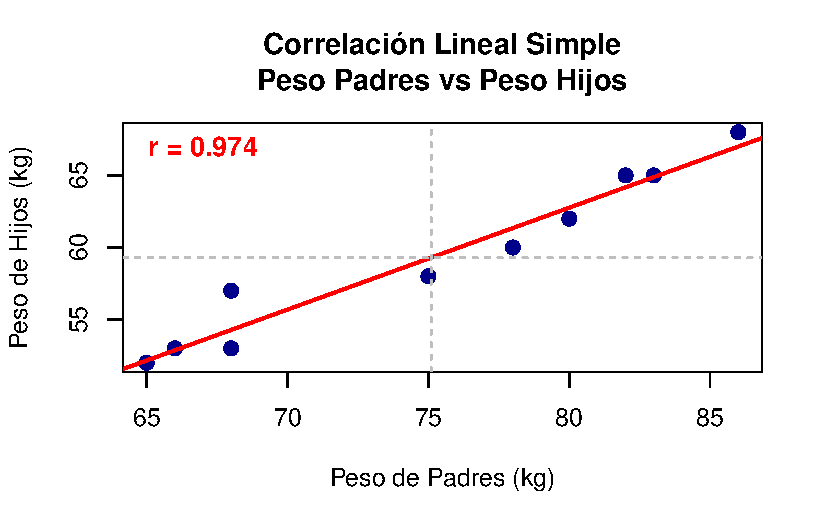
\includegraphics[keepaspectratio]{C11.1_files/figure-pdf/unnamed-chunk-6-1.pdf}}

\textbf{Elementos Explicativos:}

\begin{enumerate}
\def\labelenumi{\arabic{enumi}.}
\item
  \textbf{Puntos de dispersión}: Cada punto representa un par de
  observaciones (xi, yi)
\item
  \textbf{Línea de regresión}: Muestra la tendencia lineal de los datos
\item
  \textbf{Líneas de medias}: Indican los valores promedio de cada
  variable
\item
  \textbf{Coeficiente de correlación}: Cuantifica la fuerza de la
  asociación lineal
\end{enumerate}

\subsection{Gráfico con Intervalos de
Confianza}\label{gruxe1fico-con-intervalos-de-confianza}

Este gráfico avanzado incorpora bandas de confianza que indican la
incertidumbre asociada con la línea de regresión estimada.

\begin{Shaded}
\begin{Highlighting}[]
\CommentTok{\# 2. Gráfico con intervalos de confianza}
\FunctionTok{plot}\NormalTok{(x, y, }
     \AttributeTok{main =} \StringTok{"Dispersión con Banda de Confianza"}\NormalTok{,}
     \AttributeTok{xlab =} \StringTok{"Peso de Padres (kg)"}\NormalTok{,}
     \AttributeTok{ylab =} \StringTok{"Peso de Hijos (kg)"}\NormalTok{,}
     \AttributeTok{pch =} \DecValTok{19}\NormalTok{, }
     \AttributeTok{col =} \StringTok{"darkgreen"}\NormalTok{,}
     \AttributeTok{cex =} \FloatTok{1.2}\NormalTok{)}

\CommentTok{\# Crear secuencia para línea suave}
\NormalTok{x\_seq }\OtherTok{\textless{}{-}} \FunctionTok{seq}\NormalTok{(}\FunctionTok{min}\NormalTok{(x), }\FunctionTok{max}\NormalTok{(x), }\AttributeTok{length.out =} \DecValTok{100}\NormalTok{)}
\NormalTok{modelo }\OtherTok{\textless{}{-}} \FunctionTok{lm}\NormalTok{(y }\SpecialCharTok{\textasciitilde{}}\NormalTok{ x)}
\NormalTok{predicciones }\OtherTok{\textless{}{-}} \FunctionTok{predict}\NormalTok{(modelo, }\AttributeTok{newdata =} \FunctionTok{data.frame}\NormalTok{(}\AttributeTok{x =}\NormalTok{ x\_seq), }
                       \AttributeTok{interval =} \StringTok{"confidence"}\NormalTok{)}

\CommentTok{\# Agregar banda de confianza}
\FunctionTok{polygon}\NormalTok{(}\FunctionTok{c}\NormalTok{(x\_seq, }\FunctionTok{rev}\NormalTok{(x\_seq)), }
        \FunctionTok{c}\NormalTok{(predicciones[,}\StringTok{"lwr"}\NormalTok{], }\FunctionTok{rev}\NormalTok{(predicciones[,}\StringTok{"upr"}\NormalTok{])),}
        \AttributeTok{col =} \FunctionTok{rgb}\NormalTok{(}\DecValTok{0}\NormalTok{, }\DecValTok{0}\NormalTok{, }\DecValTok{1}\NormalTok{, }\FloatTok{0.2}\NormalTok{), }\AttributeTok{border =} \ConstantTok{NA}\NormalTok{)}

\CommentTok{\# Línea de regresión}
\FunctionTok{lines}\NormalTok{(x\_seq, predicciones[,}\StringTok{"fit"}\NormalTok{], }\AttributeTok{col =} \StringTok{"blue"}\NormalTok{, }\AttributeTok{lwd =} \DecValTok{2}\NormalTok{)}
\end{Highlighting}
\end{Shaded}

\pandocbounded{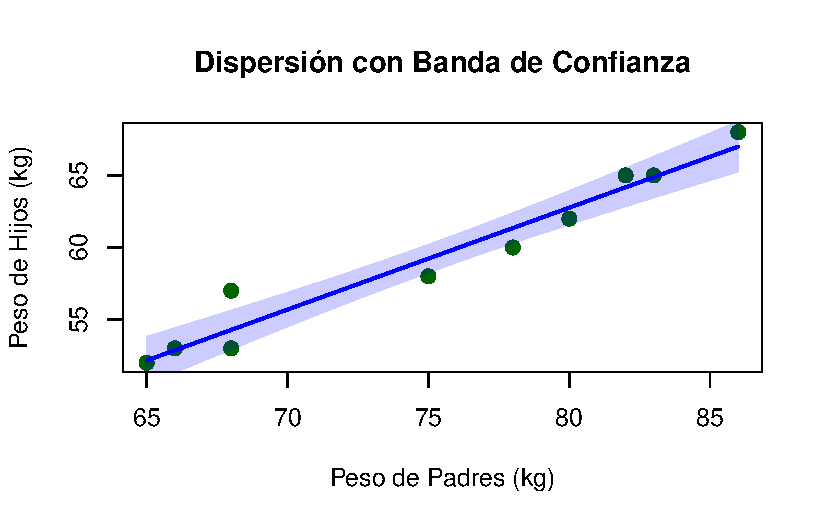
\includegraphics[keepaspectratio]{C11.1_files/figure-pdf/unnamed-chunk-7-1.pdf}}

\textbf{Interpretación:} La banda sombreada representa el intervalo de
confianza del 95\% para la línea de regresión, indicando el rango de
valores donde se espera que se encuentre la verdadera relación
poblacional.

\section{Simulación interactiva del coeficiente de
Pearson}\label{simulaciuxf3n-interactiva-del-coeficiente-de-pearson}

A continuación, se presenta una aplicación interactiva diseñada para
visualizar cómo los diferentes valores del coeficiente de correlación de
Pearson (r) se reflejan en un gráfico de dispersión junto con su
respectiva línea de tendencia. Esta herramienta facilita la comprensión
visual y práctica del concepto de correlación lineal simple, permitiendo
observar de manera dinámica cómo varía la relación entre dos variables a
medida que cambia el valor de r.

Para explorar la aplicación y experimentar con distintos escenarios de
correlación, se recomienda acceder al siguiente enlace:
\url{https://ludwing-mj.shinyapps.io/pearson/}.

\bookmarksetup{startatroot}

\chapter{Regresión Lineal Simple usando
R}\label{regresiuxf3n-lineal-simple-usando-r}

La regresión lineal simple es una técnica estadística fundamental para
analizar la relación entre dos variables cuantitativas, permitiendo
modelar y predecir el comportamiento de una variable dependiente a
partir de una variable independiente. En el contexto de la agronomía,
esta herramienta resulta esencial para comprender fenómenos como la
relación entre el peso en cultivos o animales, entre otros ejemplos
relevantes (Montgomery et al., 2021; López \& González, 2018).

\section{Fundamentos Teóricos}\label{fundamentos-teuxf3ricos-1}

El modelo de regresión lineal simple se expresa mediante la siguiente
ecuación:

\[\huge Y_i = \beta_0 + \beta_1 X_i + \varepsilon_i\]

En esta expresión:

\begin{enumerate}
\def\labelenumi{\arabic{enumi}.}
\item
  \(Y_i\) representa el valor observado de la variable dependiente para
  el individuo i.
\item
  \(X_i\) es el valor observado de la variable independiente para el
  individuo i.
\item
  \(\beta_0\) es el intercepto o constante, que indica el valor esperado
  de \(Y\) cuando \(X=0\).
\item
  \(\beta_1\) es la pendiente, que representa el cambio promedio en
  \(Y\) por cada unidad de cambio en \(X\).
\item
  \(\varepsilon_i\) es el término de error aleatorio, que recoge la
  variabilidad no explicada por el modelo.
\end{enumerate}

El objetivo de la regresión es estimar los valores de
\(\beta_0\)\hspace{0pt} y \(\beta_1\)\hspace{0pt} que mejor se ajustan a
los datos observados. Para ello, se utiliza el método de mínimos
cuadrados, que minimiza la suma de los cuadrados de las diferencias
entre los valores observados y los valores predichos por el modelo
(Montgomery et al., 2021).

Las fórmulas para los estimadores de mínimos cuadrados son:

\[\LARGE \hat{\beta_1} = \frac{\sum_{i=1}^{n} (x_i - \bar{x})(y_i - \bar{y})}{\sum_{i=1}^{n} (x_i - \bar{x})^2}\]

\[\LARGE \hat{\beta_0} = \bar{y} - \hat{\beta_1}\bar{x}\]

donde \(\bar{x}\) y \(\bar{y}\) son las medias de las variables \(X\) y
\(Y\) respectivamente.

\section{Supuestos del Modelo}\label{supuestos-del-modelo}

Para que los resultados de la regresión lineal simple sean válidos, es
necesario que se cumplan los siguientes supuestos (López \& González,
2018):

\begin{enumerate}
\def\labelenumi{\arabic{enumi}.}
\item
  \textbf{Linealidad:} La relación entre la variable independiente y la
  dependiente debe ser lineal. Esto significa que el efecto de \(X\)
  sobre \(Y\) es constante a lo largo de todo el rango de valores.
\item
  \textbf{Normalidad de los errores:} Los residuos (diferencias entre
  los valores observados y los predichos) deben seguir una distribución
  normal.
\item
  \textbf{Homocedasticidad:} La varianza de los errores debe ser
  constante para todos los valores de \(X\).
\item
  \textbf{Independencia:} Las observaciones deben ser independientes
  entre sí, es decir, el valor de una observación no debe influir en el
  valor de otra.
\end{enumerate}

El incumplimiento de estos supuestos puede llevar a conclusiones
erróneas o a una interpretación incorrecta de los resultados.

\section{Análisis Práctico en R}\label{anuxe1lisis-pruxe1ctico-en-r}

\subsection{Instalación y carga de
paquetes}\label{instalaciuxf3n-y-carga-de-paquetes-1}

El análisis inicia con la carga de los paquetes especializados y la
exploración de los datos:

\begin{Shaded}
\begin{Highlighting}[]
\CommentTok{\# Instalación y carga de paquetes necesarios}
\ControlFlowTok{if}\NormalTok{ (}\SpecialCharTok{!}\FunctionTok{require}\NormalTok{(tidyverse)) }\FunctionTok{install.packages}\NormalTok{(}\StringTok{"tidyverse"}\NormalTok{)}
\ControlFlowTok{if}\NormalTok{ (}\SpecialCharTok{!}\FunctionTok{require}\NormalTok{(car)) }\FunctionTok{install.packages}\NormalTok{(}\StringTok{"car"}\NormalTok{)}
\ControlFlowTok{if}\NormalTok{ (}\SpecialCharTok{!}\FunctionTok{require}\NormalTok{(lmtest)) }\FunctionTok{install.packages}\NormalTok{(}\StringTok{"lmtest"}\NormalTok{)}
\ControlFlowTok{if}\NormalTok{ (}\SpecialCharTok{!}\FunctionTok{require}\NormalTok{(nortest)) }\FunctionTok{install.packages}\NormalTok{(}\StringTok{"nortest"}\NormalTok{)}
\end{Highlighting}
\end{Shaded}

Se recomienda siempre inspeccionar los datos antes de analizarlos. En
este ejemplo, se utiliza un conjunto de datos ficticio sobre el peso de
padres e hijos empleado para explicar el análisis de correlación lineal:

\begin{Shaded}
\begin{Highlighting}[]
\CommentTok{\# Datos del ejemplo: peso de padres (X) y peso de hijos (Y) en kilogramos}
\NormalTok{datos }\OtherTok{\textless{}{-}} \FunctionTok{data.frame}\NormalTok{(}
  \AttributeTok{Peso\_Padres =} \FunctionTok{c}\NormalTok{(}\DecValTok{78}\NormalTok{, }\DecValTok{65}\NormalTok{, }\DecValTok{86}\NormalTok{, }\DecValTok{68}\NormalTok{, }\DecValTok{83}\NormalTok{, }\DecValTok{68}\NormalTok{, }\DecValTok{75}\NormalTok{, }\DecValTok{80}\NormalTok{, }\DecValTok{82}\NormalTok{, }\DecValTok{66}\NormalTok{),}
  \AttributeTok{Peso\_Hijos =} \FunctionTok{c}\NormalTok{(}\DecValTok{60}\NormalTok{, }\DecValTok{52}\NormalTok{, }\DecValTok{68}\NormalTok{, }\DecValTok{53}\NormalTok{, }\DecValTok{65}\NormalTok{, }\DecValTok{57}\NormalTok{, }\DecValTok{58}\NormalTok{, }\DecValTok{62}\NormalTok{, }\DecValTok{65}\NormalTok{, }\DecValTok{53}\NormalTok{)}
\NormalTok{)}
\end{Highlighting}
\end{Shaded}

Es recomendable graficar los datos para observar la posible relación
lineal:

\begin{Shaded}
\begin{Highlighting}[]
\CommentTok{\# Gráfico de dispersión}
\FunctionTok{ggplot}\NormalTok{(datos, }\FunctionTok{aes}\NormalTok{(}\AttributeTok{x =}\NormalTok{ Peso\_Padres, }\AttributeTok{y =}\NormalTok{ Peso\_Hijos)) }\SpecialCharTok{+}
  \FunctionTok{geom\_point}\NormalTok{() }\SpecialCharTok{+}
  \FunctionTok{labs}\NormalTok{(}\AttributeTok{title =} \StringTok{"Relación entre el peso de padres e hijos"}\NormalTok{,}
       \AttributeTok{x =} \StringTok{"Peso de padres (kg)"}\NormalTok{,}
       \AttributeTok{y =} \StringTok{"Peso de hijos (kg)"}\NormalTok{)}
\end{Highlighting}
\end{Shaded}

\pandocbounded{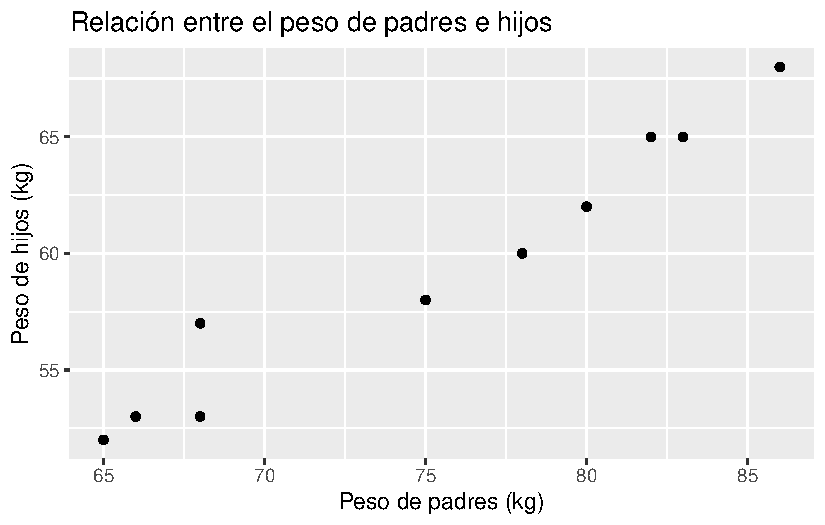
\includegraphics[keepaspectratio]{C11.2_files/figure-pdf/unnamed-chunk-3-1.pdf}}

\subsection{Ajuste del Modelo}\label{ajuste-del-modelo}

Para ajustar el modelo, se utiliza la función \texttt{lm()}, cuya
sintaxis general es:

\begin{Shaded}
\begin{Highlighting}[]
\NormalTok{modelo }\OtherTok{\textless{}{-}} \FunctionTok{lm}\NormalTok{(Y }\SpecialCharTok{\textasciitilde{}}\NormalTok{ X, }\AttributeTok{data =}\NormalTok{ datos)}
\end{Highlighting}
\end{Shaded}

En este caso:

\begin{Shaded}
\begin{Highlighting}[]
\NormalTok{modelo }\OtherTok{\textless{}{-}} \FunctionTok{lm}\NormalTok{(Peso\_Hijos }\SpecialCharTok{\textasciitilde{}}\NormalTok{ Peso\_Padres, }\AttributeTok{data =}\NormalTok{ datos)}
\end{Highlighting}
\end{Shaded}

Para obtener un resumen detallado del modelo, se emplea:

\begin{Shaded}
\begin{Highlighting}[]
\FunctionTok{summary}\NormalTok{(modelo)}
\end{Highlighting}
\end{Shaded}

\begin{verbatim}

Call:
lm(formula = Peso_Hijos ~ Peso_Padres, data = datos)

Residuals:
     Min       1Q   Median       3Q      Max 
-1.35052 -1.11314 -0.02222  0.64948  2.72024 

Coefficients:
            Estimate Std. Error t value Pr(>|t|)    
(Intercept)  6.19857    4.37024   1.418    0.194    
Peso_Padres  0.70708    0.05791  12.209 1.88e-06 ***
---
Signif. codes:  0 '***' 0.001 '**' 0.01 '*' 0.05 '.' 0.1 ' ' 1

Residual standard error: 1.354 on 8 degrees of freedom
Multiple R-squared:  0.9491,    Adjusted R-squared:  0.9427 
F-statistic: 149.1 on 1 and 8 DF,  p-value: 1.879e-06
\end{verbatim}

El resumen incluye los coeficientes estimados, sus errores estándar,
valores t y p, así como el coeficiente de determinación (\(R^2\)), que
indica la proporción de la variabilidad de \(Y\) explicada por \(X\).

\subsection{Evaluación Crítica de
Supuestos}\label{evaluaciuxf3n-cruxedtica-de-supuestos}

\subsubsection{Supuesto de Linealidad}\label{supuesto-de-linealidad}

Se evalúa mediante el gráfico de residuos vs valores ajustados. Si los
residuos se distribuyen aleatoriamente alrededor de cero, el supuesto se
considera cumplido.

\begin{Shaded}
\begin{Highlighting}[]
\FunctionTok{plot}\NormalTok{(modelo, }\AttributeTok{which =} \DecValTok{1}\NormalTok{)  }\CommentTok{\# Residuals vs Fitted}
\end{Highlighting}
\end{Shaded}

\pandocbounded{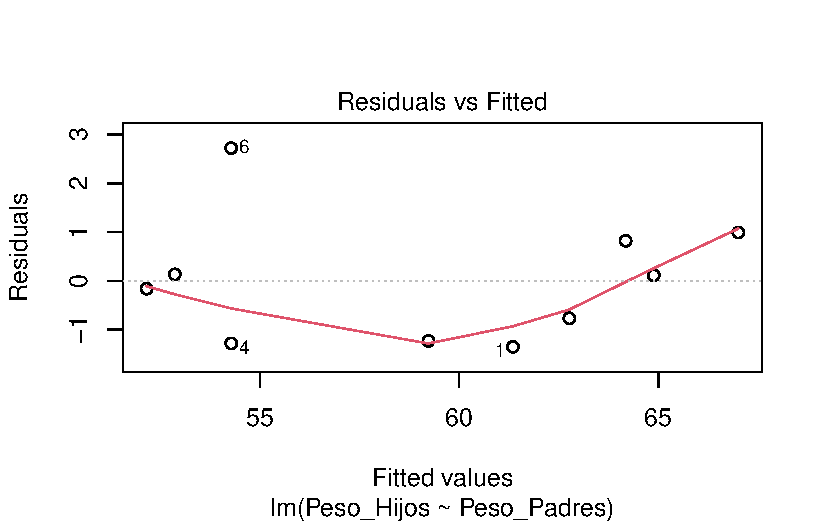
\includegraphics[keepaspectratio]{C11.2_files/figure-pdf/unnamed-chunk-7-1.pdf}}

\subsubsection{Supuesto de Normalidad}\label{supuesto-de-normalidad}

Se puede evaluar visualmente con un gráfico Q-Q y mediante pruebas
estadísticas como Shapiro-Wilk y Anderson-Darling:

\textbf{Gráfico Q-Q:}

\begin{Shaded}
\begin{Highlighting}[]
\CommentTok{\# Gráfico Q{-}Q}
\FunctionTok{plot}\NormalTok{(modelo, }\AttributeTok{which =} \DecValTok{2}\NormalTok{)  }\CommentTok{\# Normal Q{-}Q}
\end{Highlighting}
\end{Shaded}

\pandocbounded{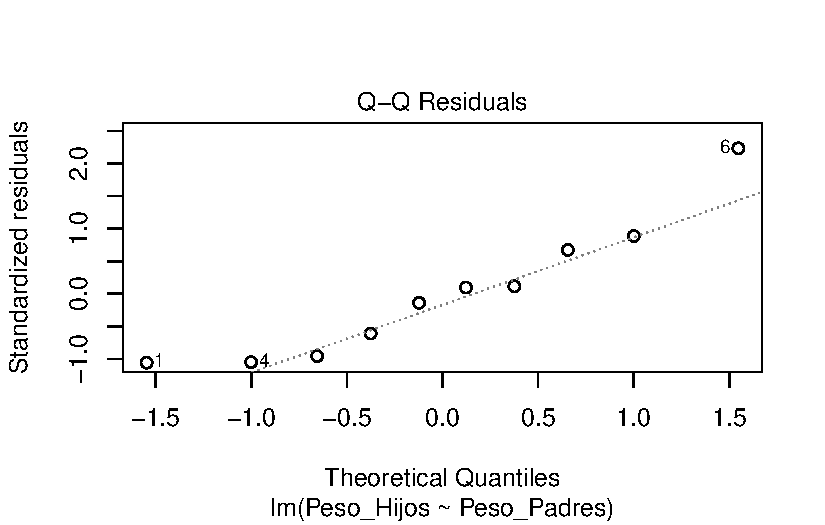
\includegraphics[keepaspectratio]{C11.2_files/figure-pdf/unnamed-chunk-8-1.pdf}}

\textbf{Prueba de Shapiro-Wilk:}

\begin{enumerate}
\def\labelenumi{\arabic{enumi}.}
\item
  \(H_0​\): Los residuos siguen distribución normal
\item
  \(H_a\)\hspace{0pt}: Los residuos no siguen distribución normal
\end{enumerate}

\begin{Shaded}
\begin{Highlighting}[]
\FunctionTok{shapiro.test}\NormalTok{(}\FunctionTok{residuals}\NormalTok{(modelo))}
\end{Highlighting}
\end{Shaded}

\begin{verbatim}

    Shapiro-Wilk normality test

data:  residuals(modelo)
W = 0.9049, p-value = 0.2478
\end{verbatim}

\textbf{Prueba de Anderson-Darling} (más potente para muestras grandes):

\begin{Shaded}
\begin{Highlighting}[]
\FunctionTok{ad.test}\NormalTok{(}\FunctionTok{residuals}\NormalTok{(modelo))}
\end{Highlighting}
\end{Shaded}

\begin{verbatim}

    Anderson-Darling normality test

data:  residuals(modelo)
A = 0.36544, p-value = 0.3604
\end{verbatim}

\subsubsection{Supuesto de
Homocedasticidad}\label{supuesto-de-homocedasticidad}

Se evalúa con la \textbf{Prueba de Breusch-Pagan:}

\begin{enumerate}
\def\labelenumi{\arabic{enumi}.}
\item
  \(H_0\)\hspace{0pt}: Varianza constante (homocedasticidad)
\item
  \(H_a\)\hspace{0pt}: Varianza no constante (heterocedasticidad)
\end{enumerate}

\begin{Shaded}
\begin{Highlighting}[]
\FunctionTok{bptest}\NormalTok{(modelo)}
\end{Highlighting}
\end{Shaded}

\begin{verbatim}

    studentized Breusch-Pagan test

data:  modelo
BP = 0.71286, df = 1, p-value = 0.3985
\end{verbatim}

\subsubsection{Supuesto de
independencia}\label{supuesto-de-independencia}

En estudios experimentales, la independencia suele garantizarse mediante
un diseño adecuado. En estudios observacionales, se recomienda analizar
el contexto y, si es posible, realizar pruebas adicionales.

\section{Predicción con el modelo
ajustado}\label{predicciuxf3n-con-el-modelo-ajustado}

Una vez ajustado el modelo, se pueden realizar predicciones para nuevos
valores de la variable independiente:

\begin{Shaded}
\begin{Highlighting}[]
\CommentTok{\# Nuevos valores de Peso\_Padres}
\NormalTok{nuevos\_pesos }\OtherTok{\textless{}{-}} \FunctionTok{data.frame}\NormalTok{(}\AttributeTok{Peso\_Padres =} \FunctionTok{c}\NormalTok{(}\DecValTok{60}\NormalTok{, }\DecValTok{75}\NormalTok{, }\DecValTok{80}\NormalTok{))}

\CommentTok{\# Predicción con intervalos de predicción}
\NormalTok{predicciones }\OtherTok{\textless{}{-}} \FunctionTok{predict}\NormalTok{(modelo, nuevos\_pesos, }\AttributeTok{interval =} \StringTok{"prediction"}\NormalTok{)}
\NormalTok{predicciones}
\end{Highlighting}
\end{Shaded}

\begin{verbatim}
       fit      lwr      upr
1 48.62315 44.77666 52.46963
2 59.22929 55.95375 62.50484
3 62.76467 59.42443 66.10492
\end{verbatim}

El resultado incluye el valor predicho y los límites inferior y superior
del intervalo de predicción para cada nuevo valor.

\section{Interpretación de
Resultados}\label{interpretaciuxf3n-de-resultados-1}

\subsection{Coeficientes del Modelo}\label{coeficientes-del-modelo}

\begin{enumerate}
\def\labelenumi{\arabic{enumi}.}
\item
  \textbf{Intercepto (}\(\hat{\beta_0}\)\hspace{0pt}): Valor esperado de
  Y cuando X = 0
\item
  \textbf{Pendiente (}\(\hat{\beta_1}\)\hspace{0pt}): Cambio promedio en
  Y por unidad de cambio en X
\end{enumerate}

\subsection{Bondad de Ajuste}\label{bondad-de-ajuste}

El \textbf{coeficiente de determinación} (\(R^2\)) indica la proporción
de variabilidad explicada:

\[\huge R^2 = \frac{SC_{Regresión}}{SC_{Total}}\]

\hspace{0pt}

\begin{enumerate}
\def\labelenumi{\arabic{enumi}.}
\item
  \(R^2 > 0.7\): Ajuste bueno
\item
  \(-0.5 < R^2 < 0.7\): Ajuste moderado
\item
  \(R^2 < 0.5\): Ajuste pobre
\end{enumerate}

\subsection{Significancia
Estadística}\label{significancia-estaduxedstica}

La \textbf{prueba F global} evalúa:

\begin{enumerate}
\def\labelenumi{\arabic{enumi}.}
\item
  \(H_0\)\hspace{0pt}: \(\beta_1 = 0\) (no hay relación lineal)
\item
  \(H_a\)\hspace{0pt}: \(\beta_1 \neq 0\) (existe relación lineal)
\end{enumerate}

\subsection{Criterios de Decisión para los
supuestos}\label{criterios-de-decisiuxf3n-para-los-supuestos}

\begin{longtable}[]{@{}lll@{}}
\toprule\noalign{}
Supuesto & Prueba & Criterio de Aceptación \\
\midrule\noalign{}
\endhead
\bottomrule\noalign{}
\endlastfoot
Normalidad & Shapiro-Wilk & p-valor \textgreater{} 0.05 \\
Homocedasticidad & Breusch-Pagan & p-valor \textgreater{} 0.05 \\
Linealidad & Gráfico residuos & Patrón aleatorio \\
Independencia & Contexto experimental & Diseño adecuado \\
\end{longtable}

\subsection{Pasos para una Interpretación Integral y
Conclusiones}\label{pasos-para-una-interpretaciuxf3n-integral-y-conclusiones}

\begin{enumerate}
\def\labelenumi{\arabic{enumi}.}
\item
  \textbf{Evaluar significancia del modelo} (prueba F global)
\item
  \textbf{Verificar supuestos} mediante pruebas estadísticas y gráficos
\item
  \textbf{Interpretar coeficientes} en el contexto del problema
\item
  \textbf{Evaluar bondad de ajuste} (\(R^2\) y \(R^2\) ajustado)
\item
  \textbf{Identificar limitaciones} del modelo
\item
  \textbf{Formular recomendaciones} prácticas
\end{enumerate}

\part{Referencias}

\bookmarksetup{startatroot}

\chapter*{Referencias}\label{referencias-1}
\addcontentsline{toc}{chapter}{Referencias}

\markboth{Referencias}{Referencias}

Hogg, R. V., McKean, J. W., \& Craig, A. T. (2019). \emph{Introduction
to mathematical statistics} (8th ed.). Pearson.

Ihaka, R., \& Gentleman, R. (1996). R: A language for data analysis and
graphics. \emph{Journal of Computational and Graphical Statistics},
\emph{5}(3), 299-314.

López, E., \& González, B. (2018). \emph{Notas de Estadística General}
(Edición marzo 2018). Guatemala: Universidad de San Carlos de Guatemala.

R Core Team (2023). \emph{R: A language and environment for statistical
computing}. R Foundation for Statistical Computing, Vienna, Austria. URL
\href{https://www.r-project.org/}{https://www.R-project.org/}.

Xie, Y., Allaire, J. J., \& Grolemund, G. (2018). \emph{R Markdown: The
definitive guide} (1st ed.). Chapman and Hall/CRC.
\url{https://doi.org/10.1201/9781138359444}

Conover, W. J. (1999). \emph{Practical Nonparametric Statistics} (3rd
ed.). Wiley.

Gelman, A., Carlin, J. B., Stern, H. S., Dunson, D. B., Vehtari, A., \&
Rubin, D. B. (2013). \emph{Bayesian Data Analysis} (3rd ed.). CRC Press.

Johnson, R. A., \& Wichern, D. W. (2014). \emph{Applied Multivariate
Statistical Analysis} (6th ed.). Pearson.

Montgomery, D. C. (2017). \emph{Design and analysis of experiments} (9th
ed.). Wiley.

Montgomery, D. C., \& Runger, G. C. (2018). \emph{Applied Statistics and
Probability for Engineers} (7th ed.). Wiley.

Ross, S. M. (2014). \emph{Introduction to probability and statistics for
engineers and scientists} (5th ed.). Academic Press.

Wackerly, D. D., Mendenhall, W., \& Scheaffer, R. L. (2014).
\emph{Mathematical statistics with applications} (7th ed.). Cengage.

Webster, R., \& Oliver, M. A. (2007). \emph{Geostatistics for
Environmental Scientists} (2nd ed.). Wiley.

Walpole, R. E., Myers, R. H., Myers, S. L., \& Ye, K. (2012).
\emph{Probability and Statistics for Engineers and Scientists} (9th
ed.). Pearson.


\backmatter
\printbibliography



\end{document}
